\chapter{Results} \label{chap:Results}

%The results chapter should simply present the results of applying the methods presented in the method chapter without further ado. This chapter will typically contain many graphs, tables, etc. Sometimes it is natural to discuss the results as they are presented, combining them into a `Results and Discussion' chapter, but more often they are kept separate.\\ 

The following sections presents the results for each attack type, with subsections for the detection threshold levels selected, as defined in section \ref{sec:ExpDef} 
For each attack type defined, a number of attacks specifying various delay levels, specified as a number of samples, are covered.
For each delay level, a number of figures are produced by running the simulation.
A figure showing a combined view of all three components, displaying the delayed and original signals, as well as a signal indicating the actual difference between the two signals.  Three more detailed figures follows, comparing the original and delayed signal to a similarity measure for each of the three PMU output components.

The delay functions defined, delays the input signal by the specified number of samples, in one or more steps.

% delay.step    
% 1.1
% 2.1 2.2 
% 3.1 3.2 3.3
% 4.1 4.2 4.3 4.4
% 5.1 5.2 5.3 5.4 5.5

Comments on the results are included for selected figures, whereas, interpretation of the results are deferred to chapter \ref{chap:Discussions}
%\newcommand{\locateResults}{PMUsim-figures/}

%\renewcommand{\locateResults}{PMUsim-figures/Cont/DelayOf_0}
%\section{The Delay Level of Zero}
For model verification purposes, the output for the delay level of zero is included.


\begin{small}
     \tcbox[size=normal, standard jigsaw, opacityback=0, boxrule=0pt,halign=justify]{
     Comment on the figure:}{
          \begin{itemize}
         \item      The delayed signal (blue) overlaps the original signal (red), producing a straight line, colored neither red nor blue.
         \item  The blue Normalised diff signal also overlaps the grey delay function.
          \end{itemize} }
\end{small}

\newpage


\begin{table}[]
\caption{Results for Magnitude Output}
\begin{tabular}{c}
  \fbox{  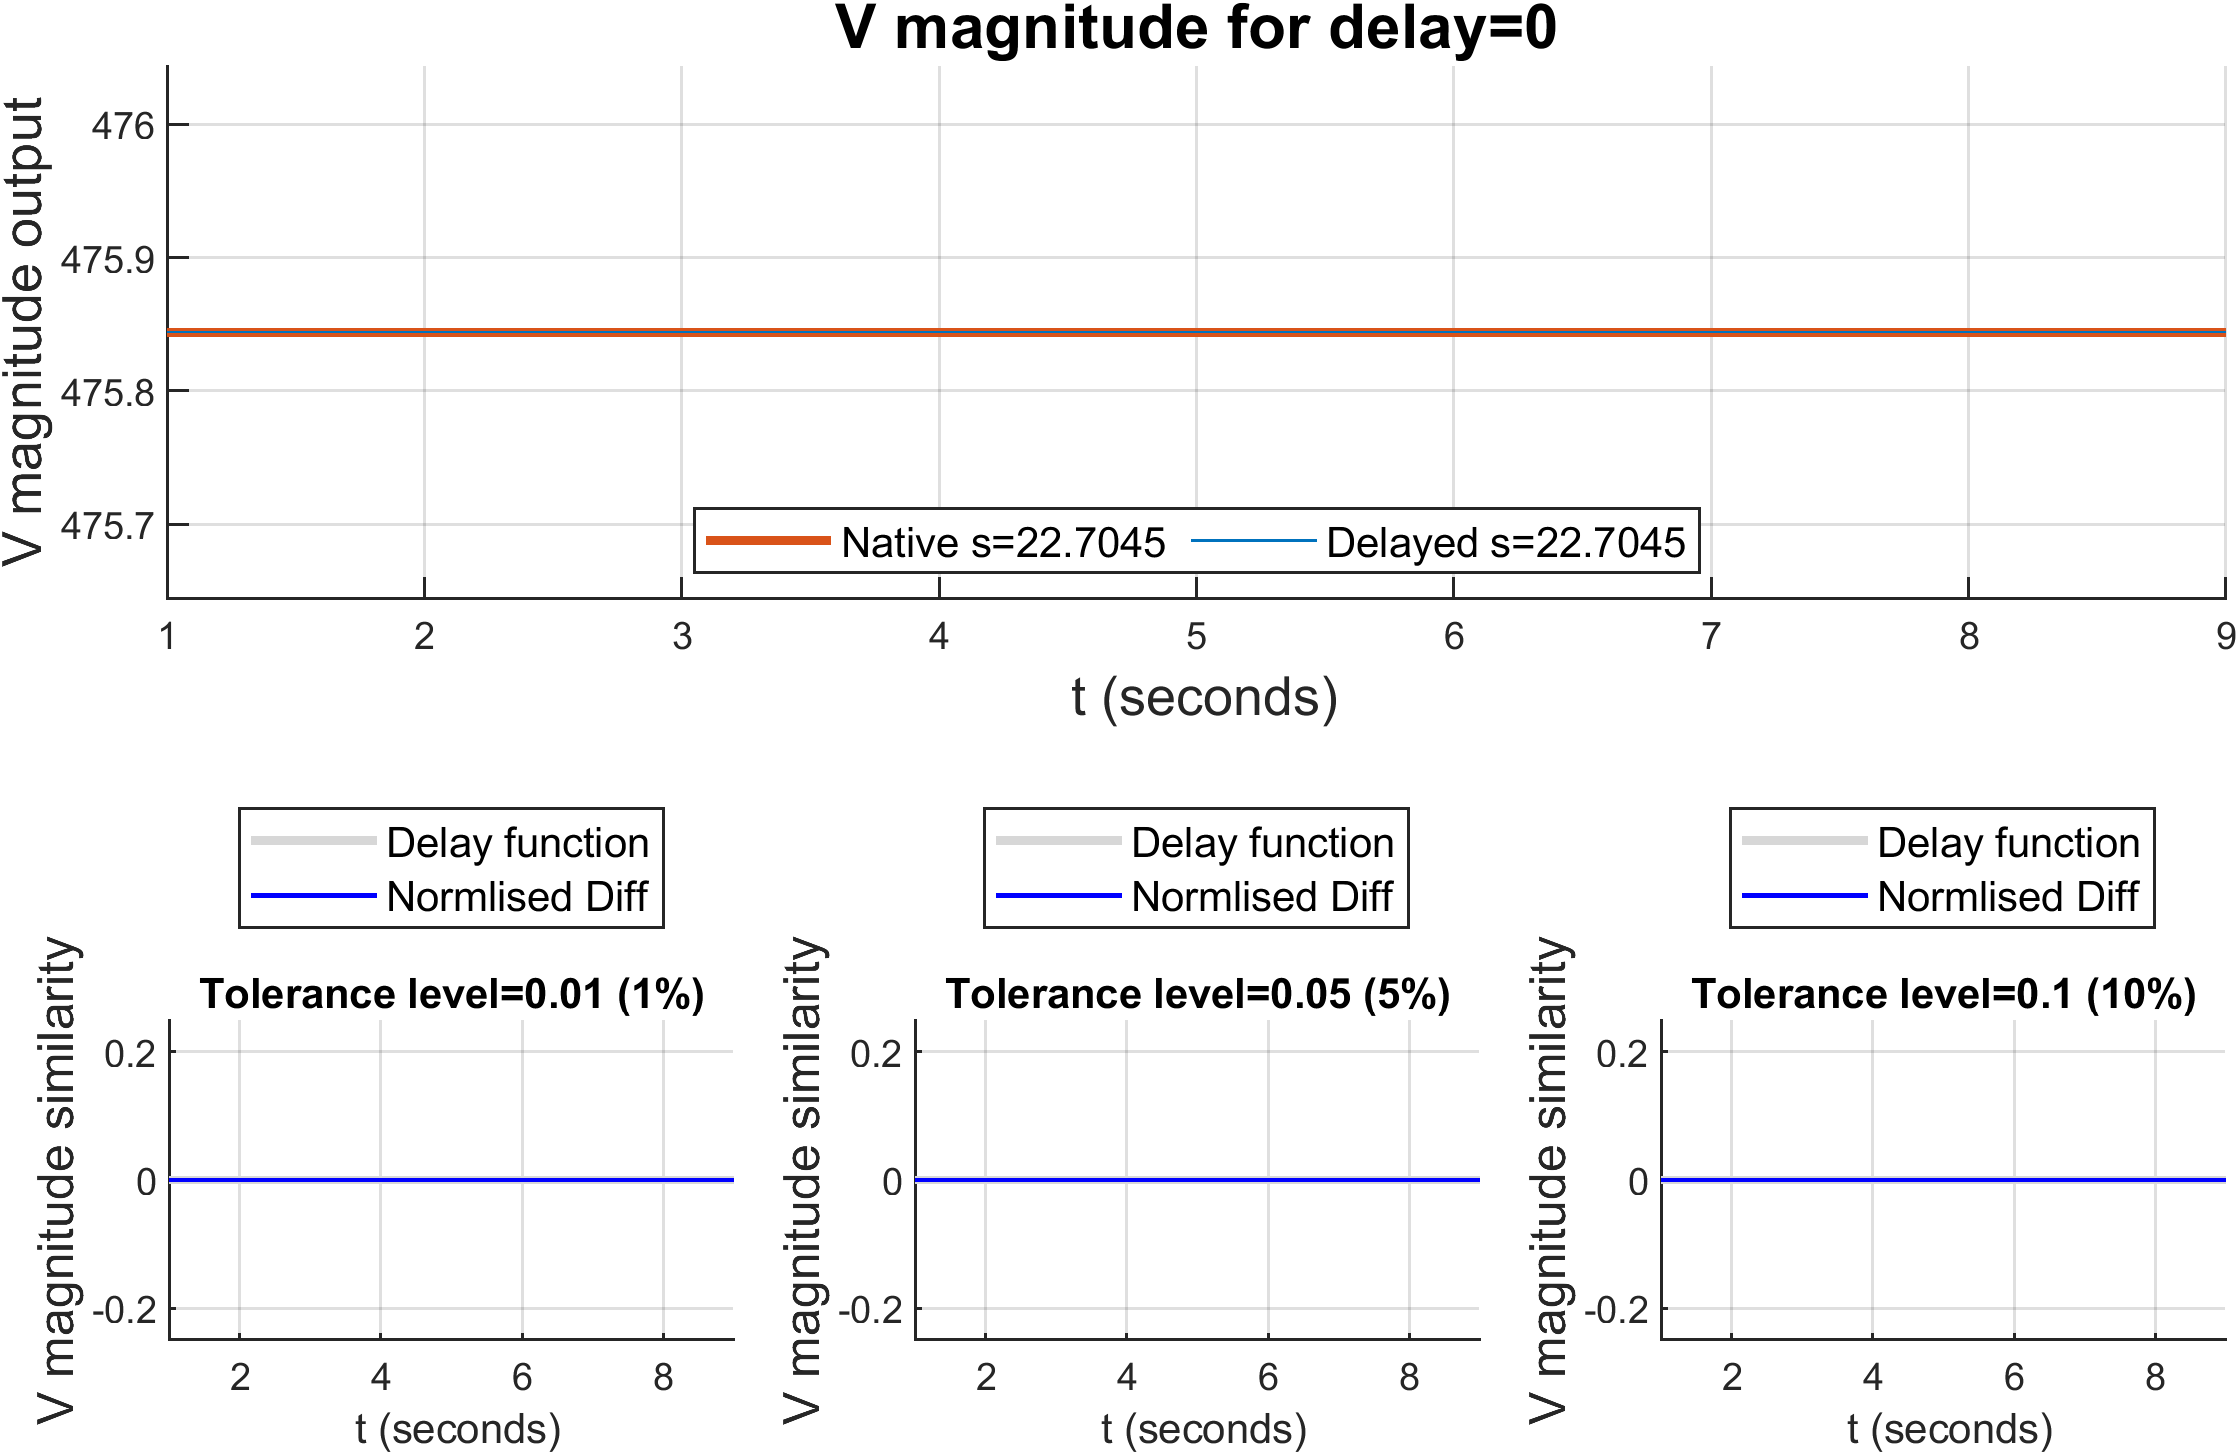
\includegraphics[width=0.95\textwidth]{PMUsim-figures/DelayOf_0/Zero_vMagnitude.png}}\
   \\
    \fbox{ 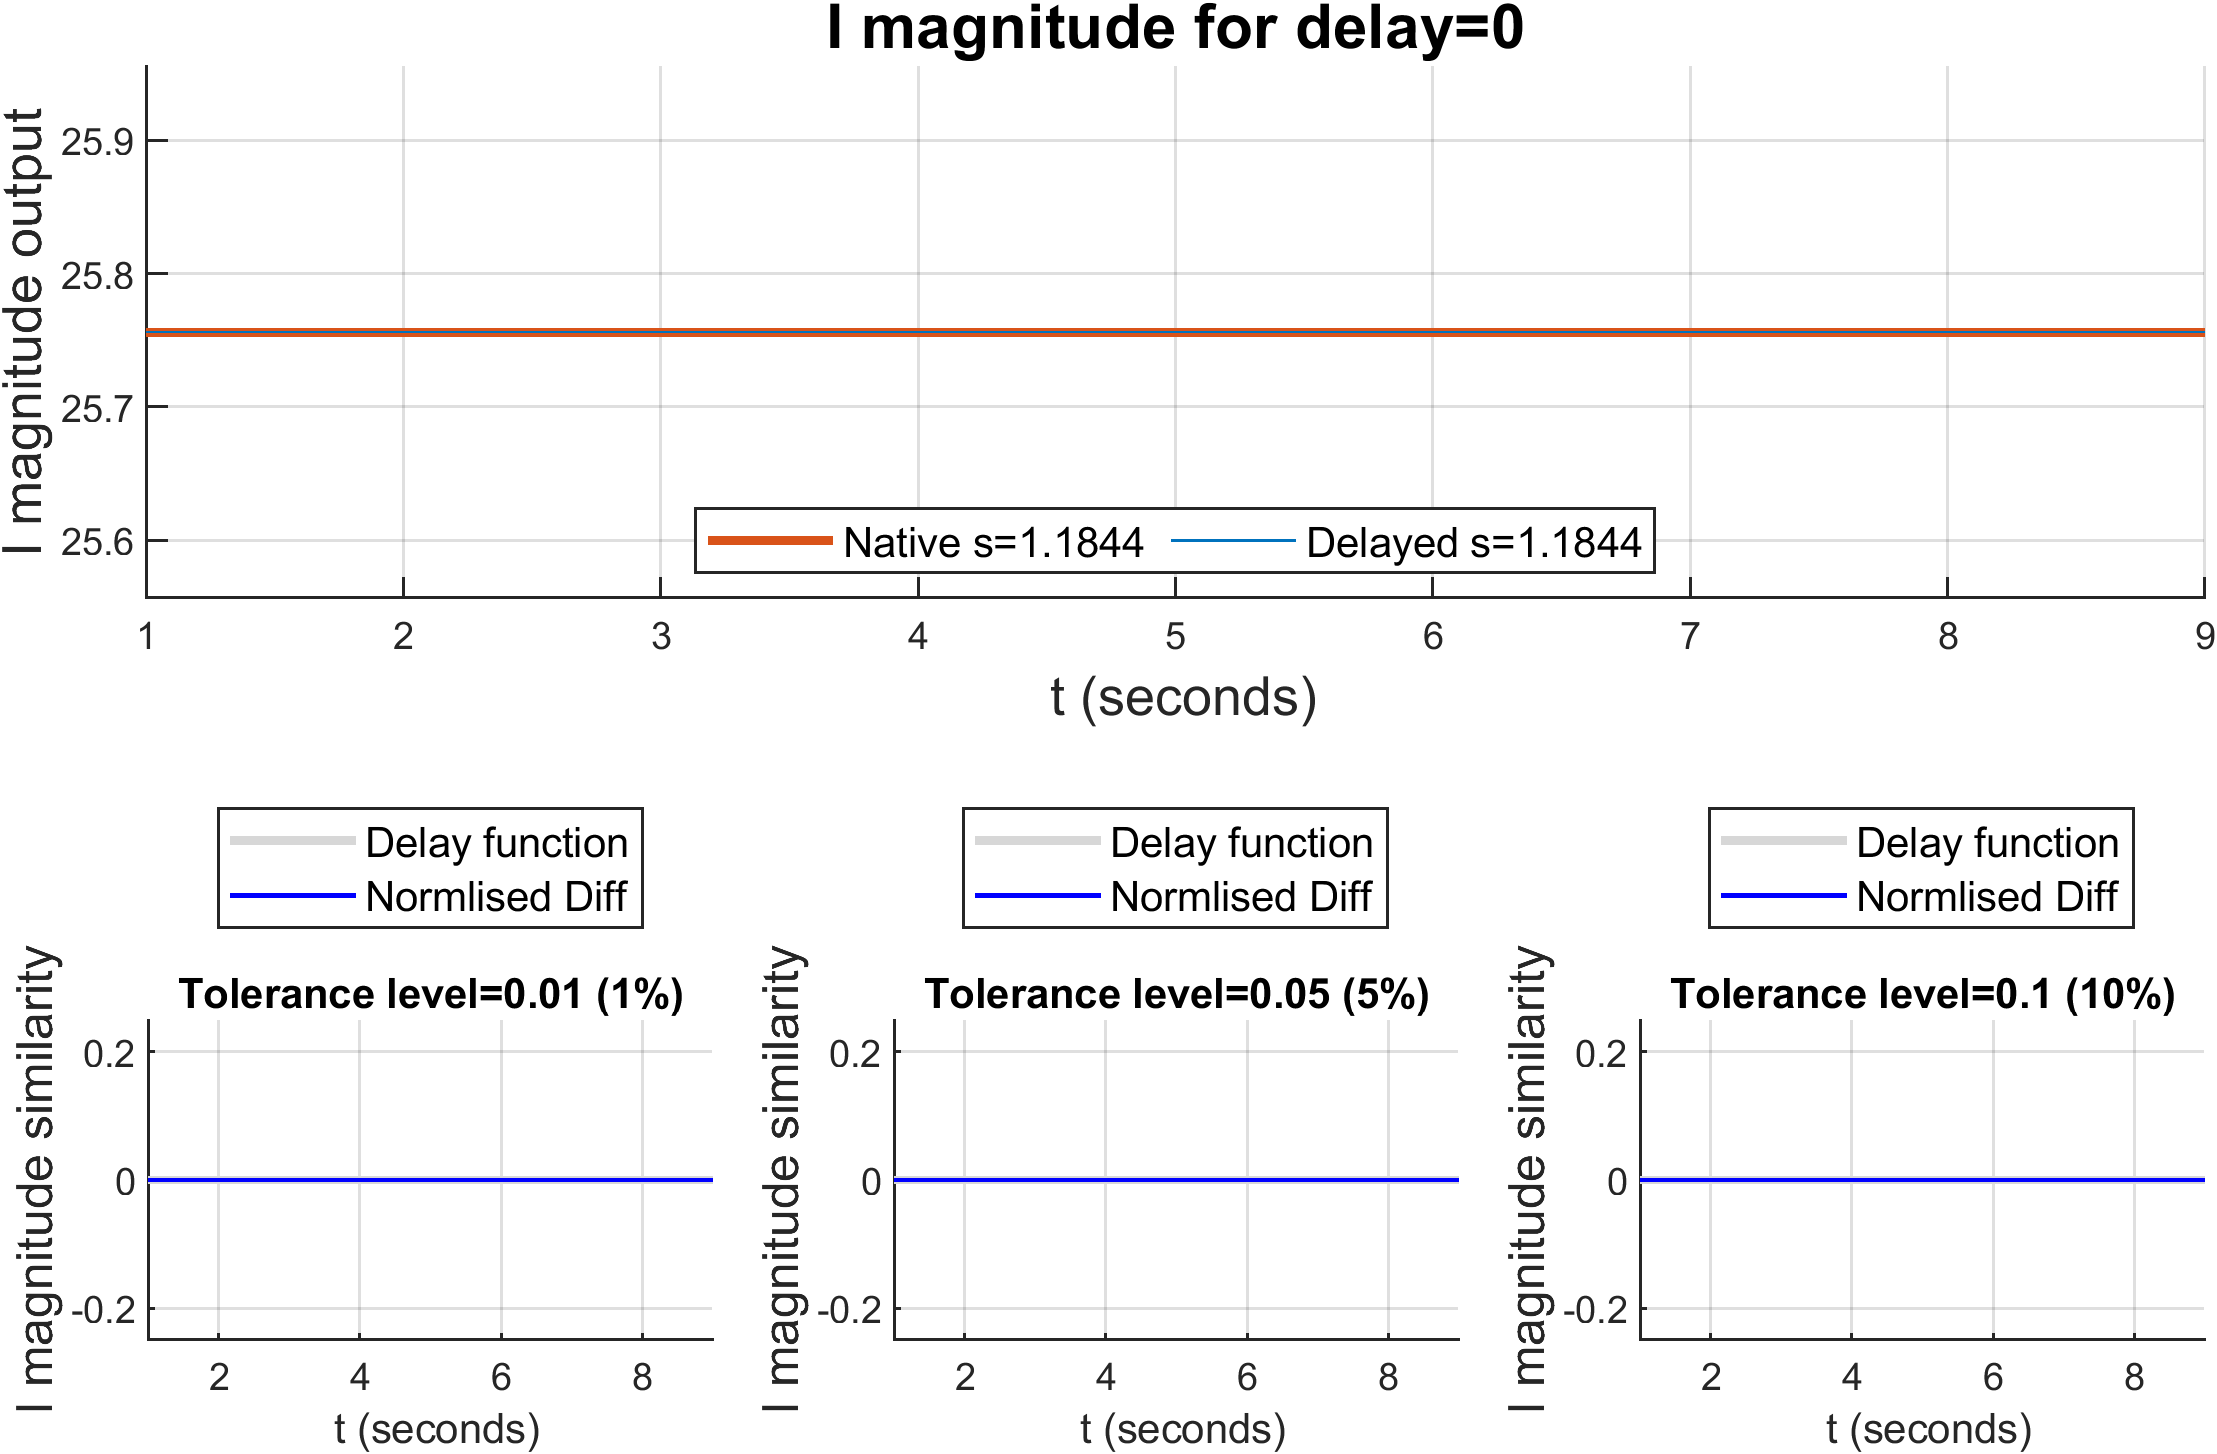
\includegraphics[width=0.95\textwidth]{PMUsim-figures/DelayOf_0/Zero_iMagnitude.png}}\
  \end{tabular}
\end{table}







  
  
\newpage 


\begin{table}[]
\caption{Results for Frequency Output}
\begin{tabular}{c}
   \fbox{    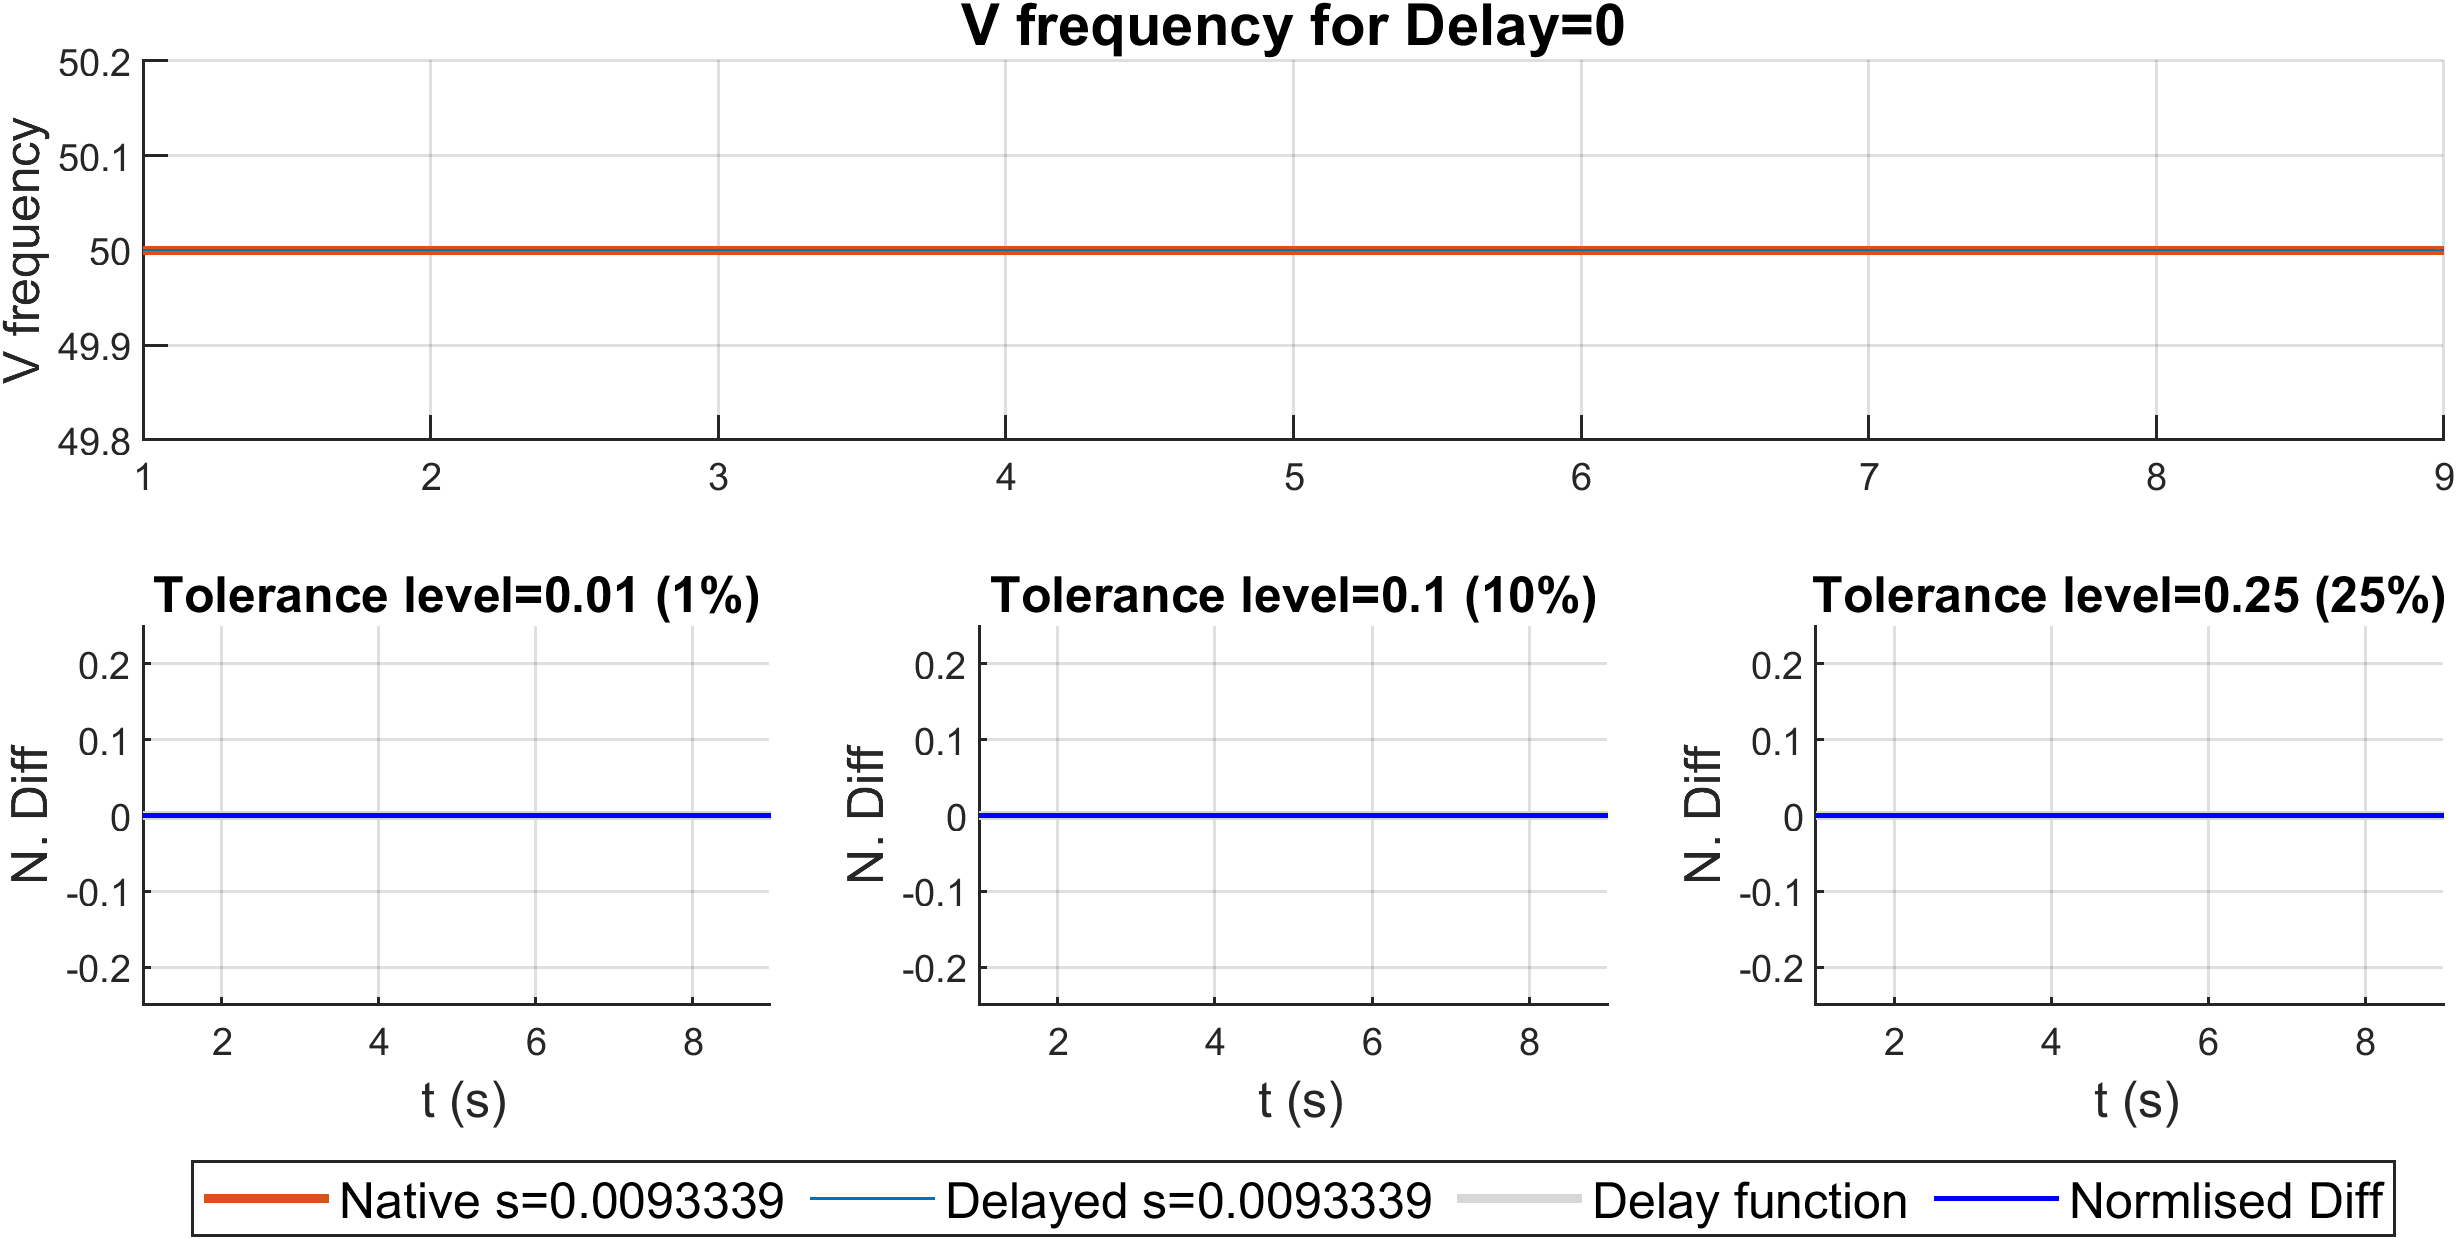
\includegraphics[width=0.95\textwidth]{PMUsim-figures/DelayOf_0/Zero_vFrequency.png}}\
  
    
   \fbox{ 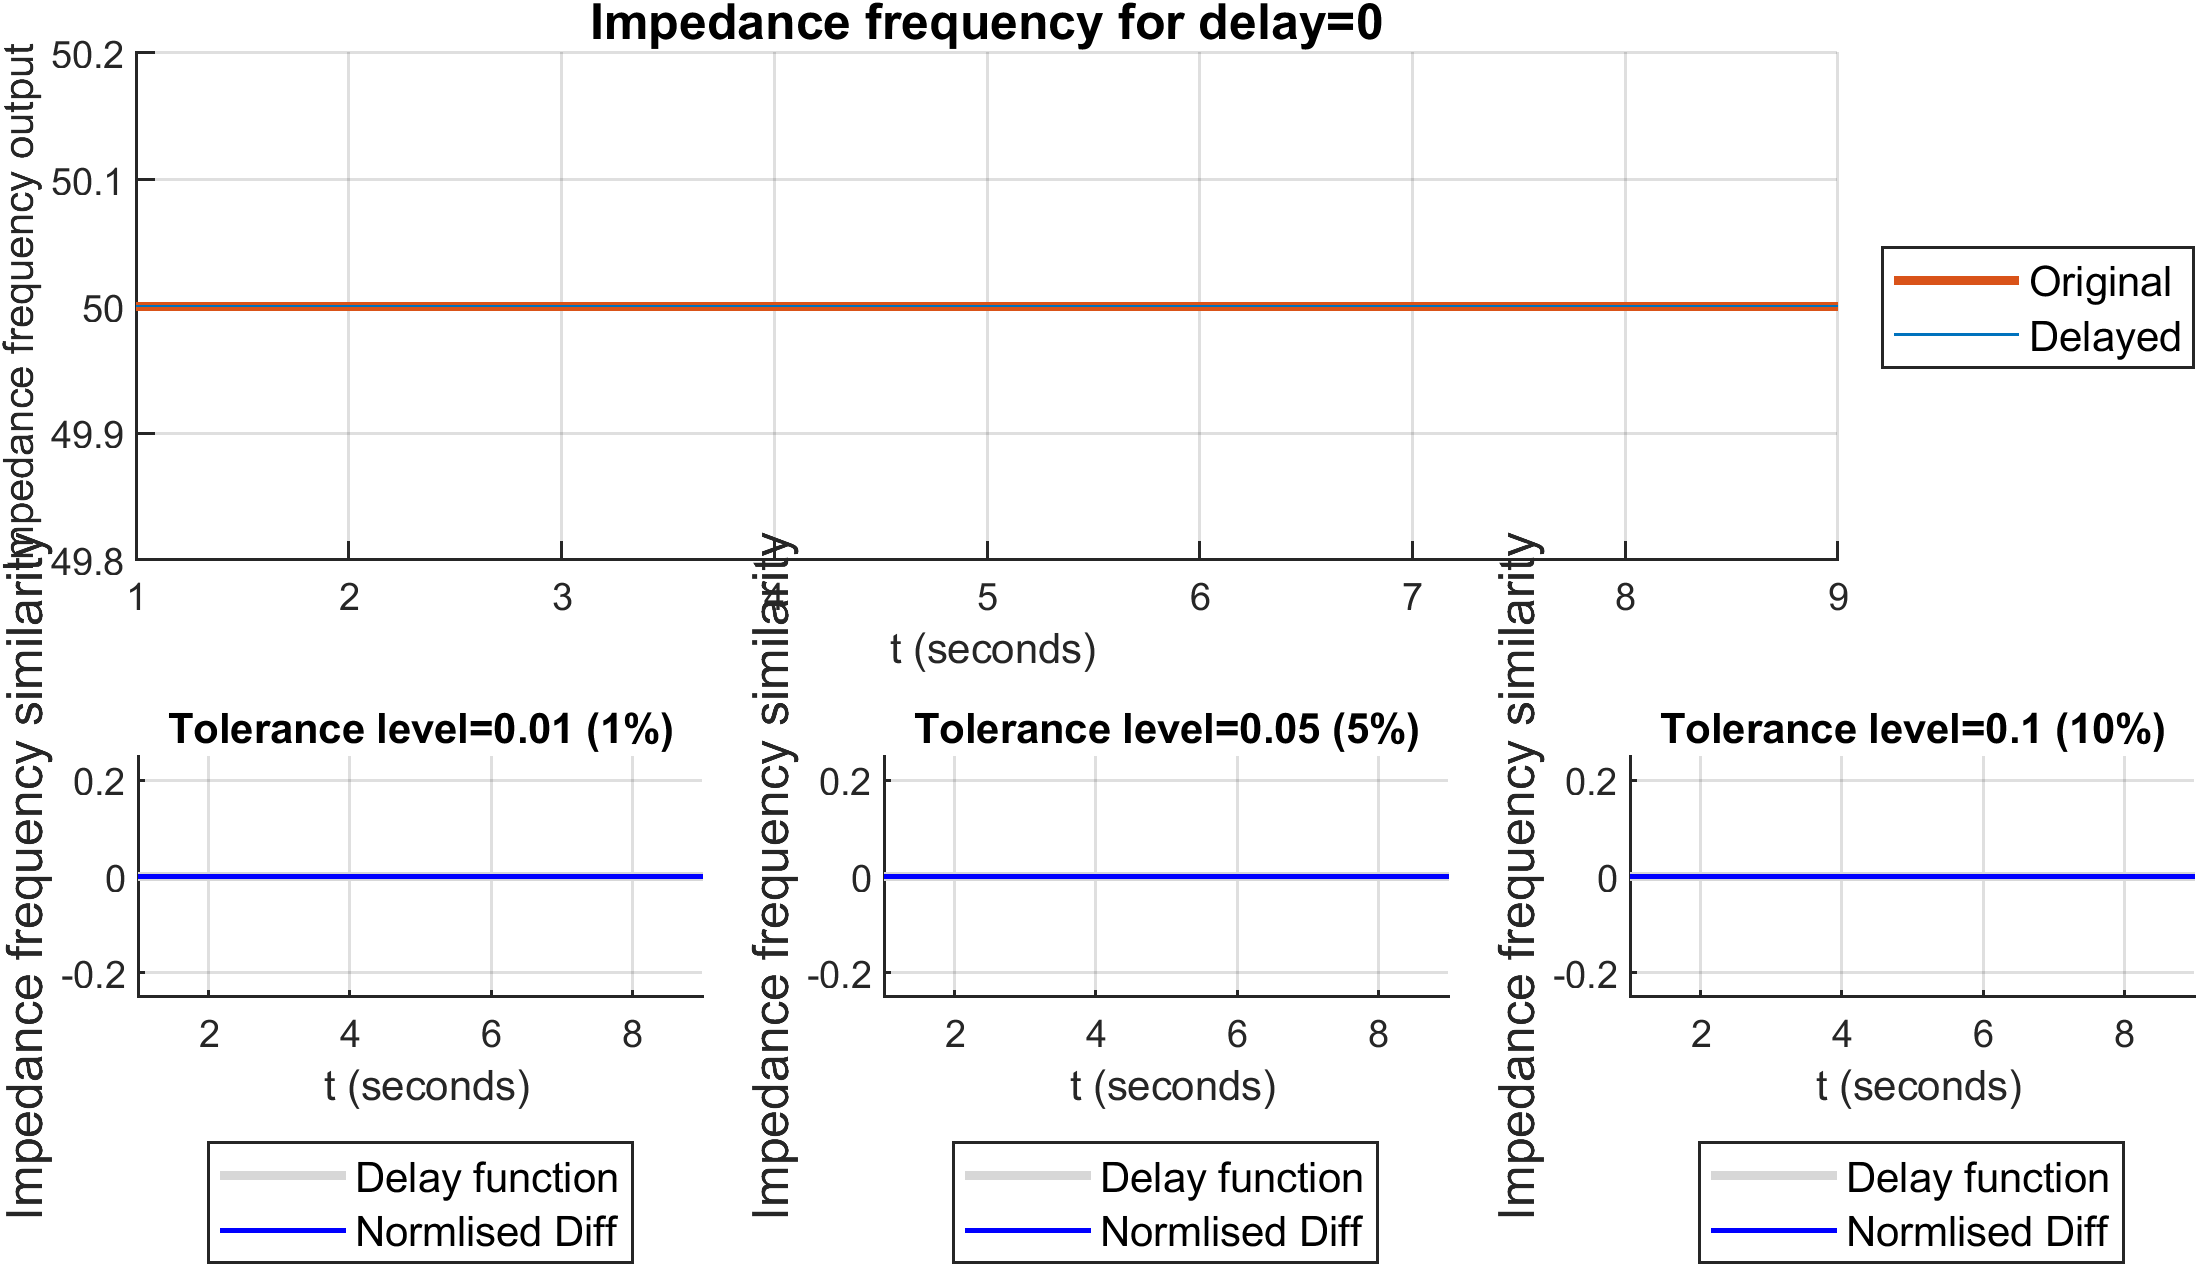
\includegraphics[width=0.95\textwidth]{PMUsim-figures/DelayOf_0/Zero_iFrequency.png}}\ 
 \label{fig:PMUsim_Zero_Frequency}
 %\caption{Zero Delay Frequency Output (for the Delay Level of Zero)}
  \end{tabular}
\end{table}



\newpage 

\begin{table}[]
\caption{Results for Angle Output}}\begin{tabular}{c}
   \fbox{     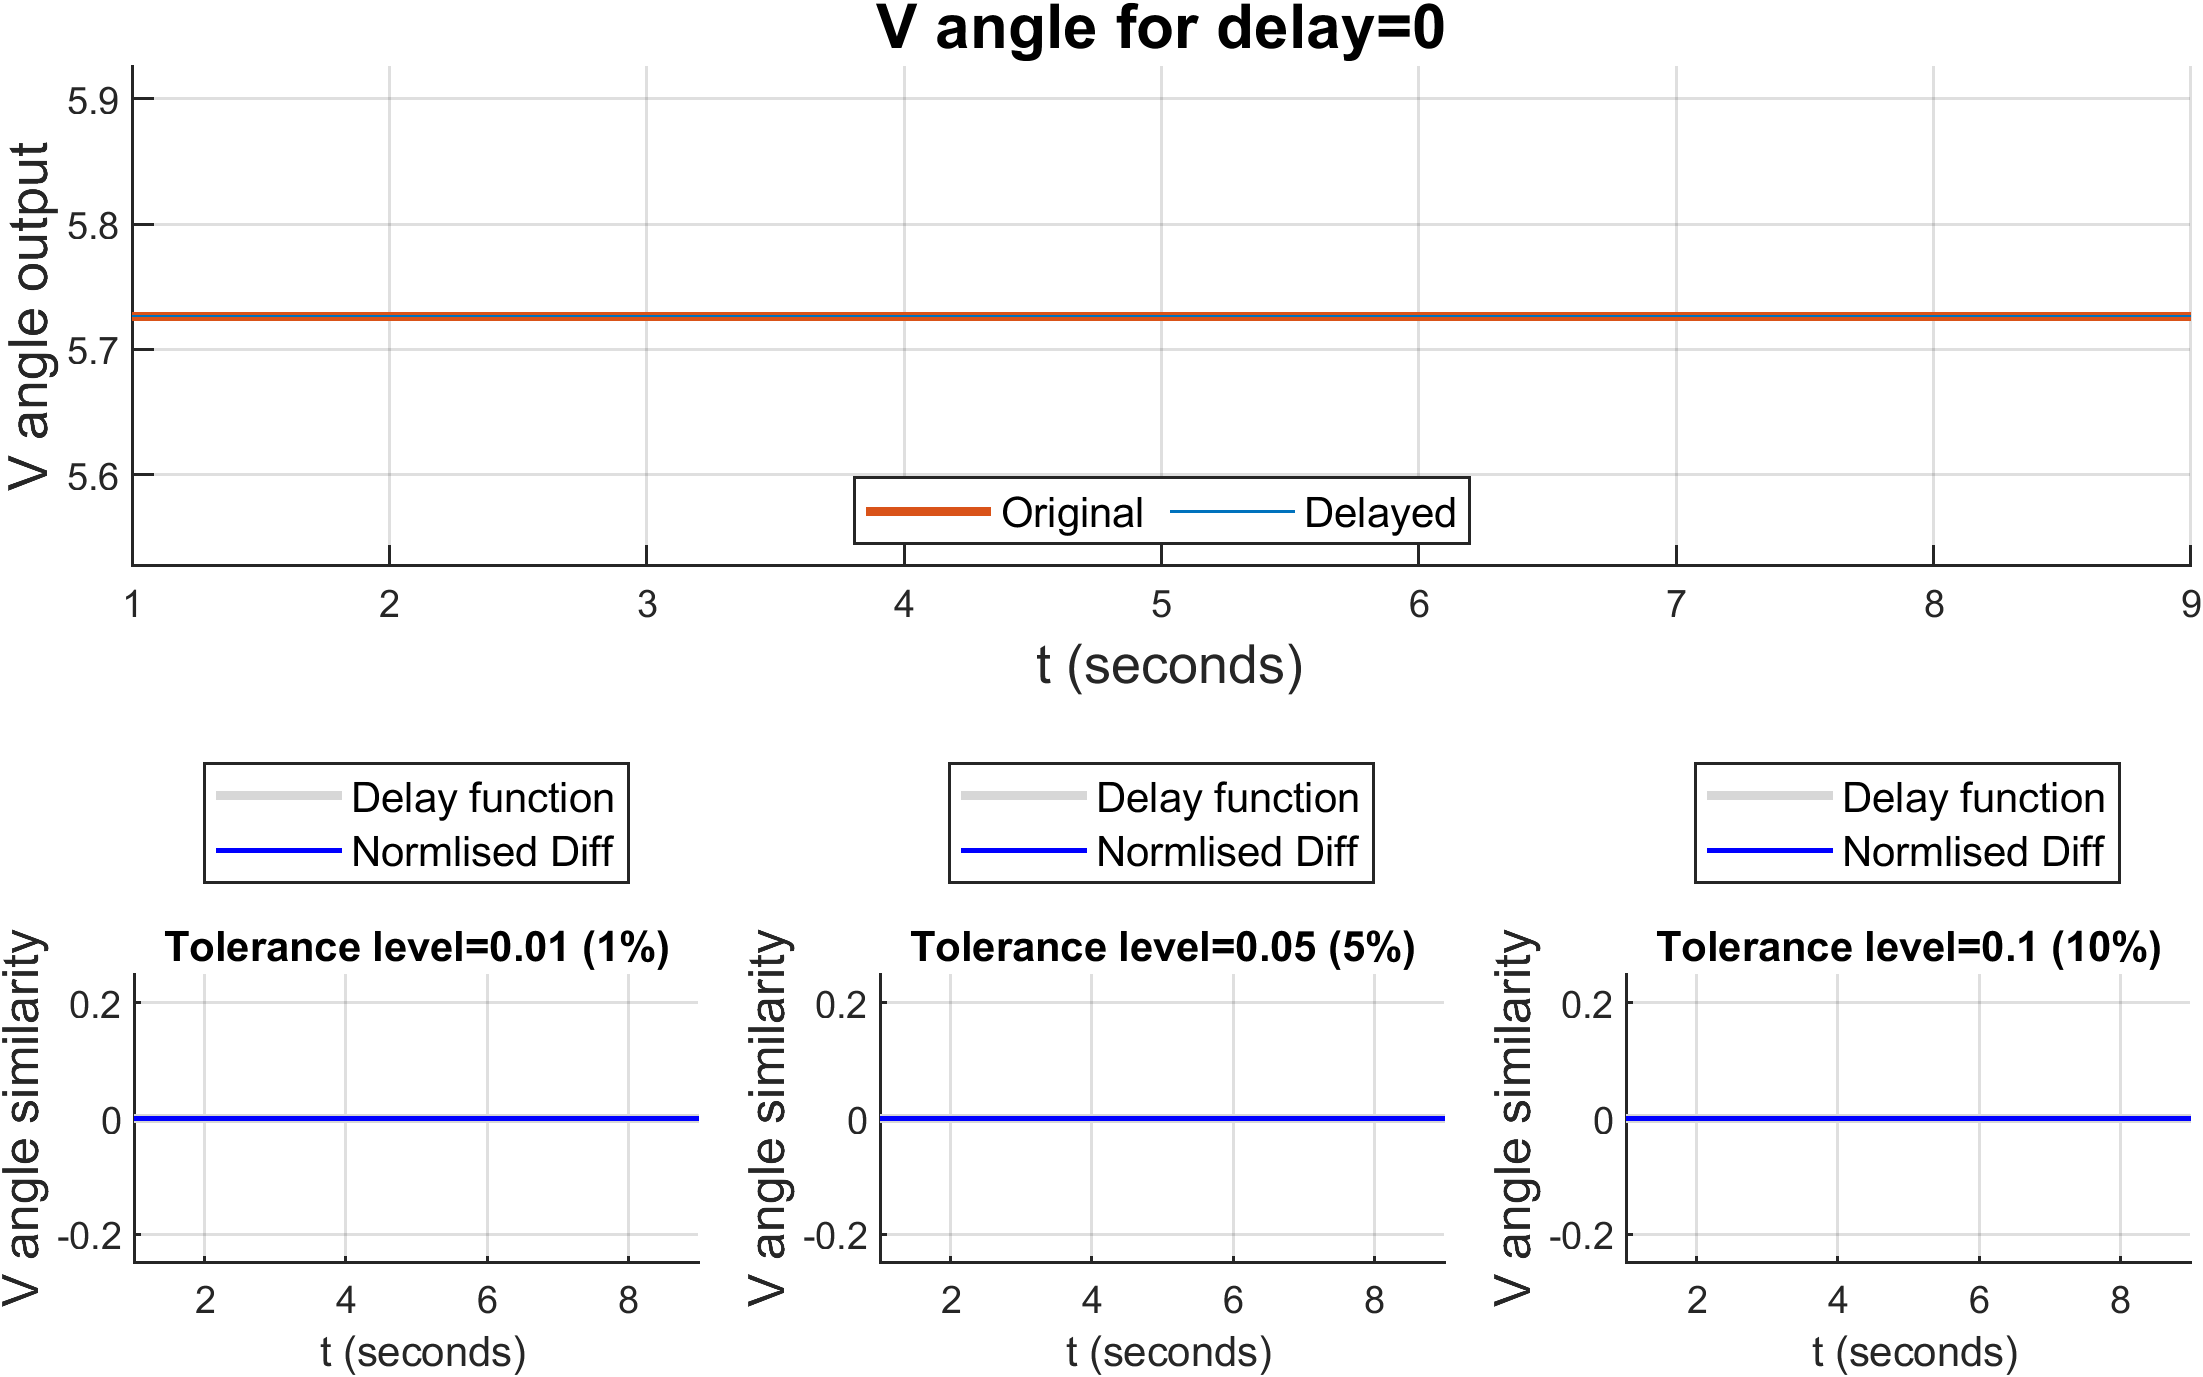
\includegraphics[width=0.95\textwidth]{PMUsim-figures/DelayOf_0/Zero_vAngle.png}}\
  
    
   \fbox{  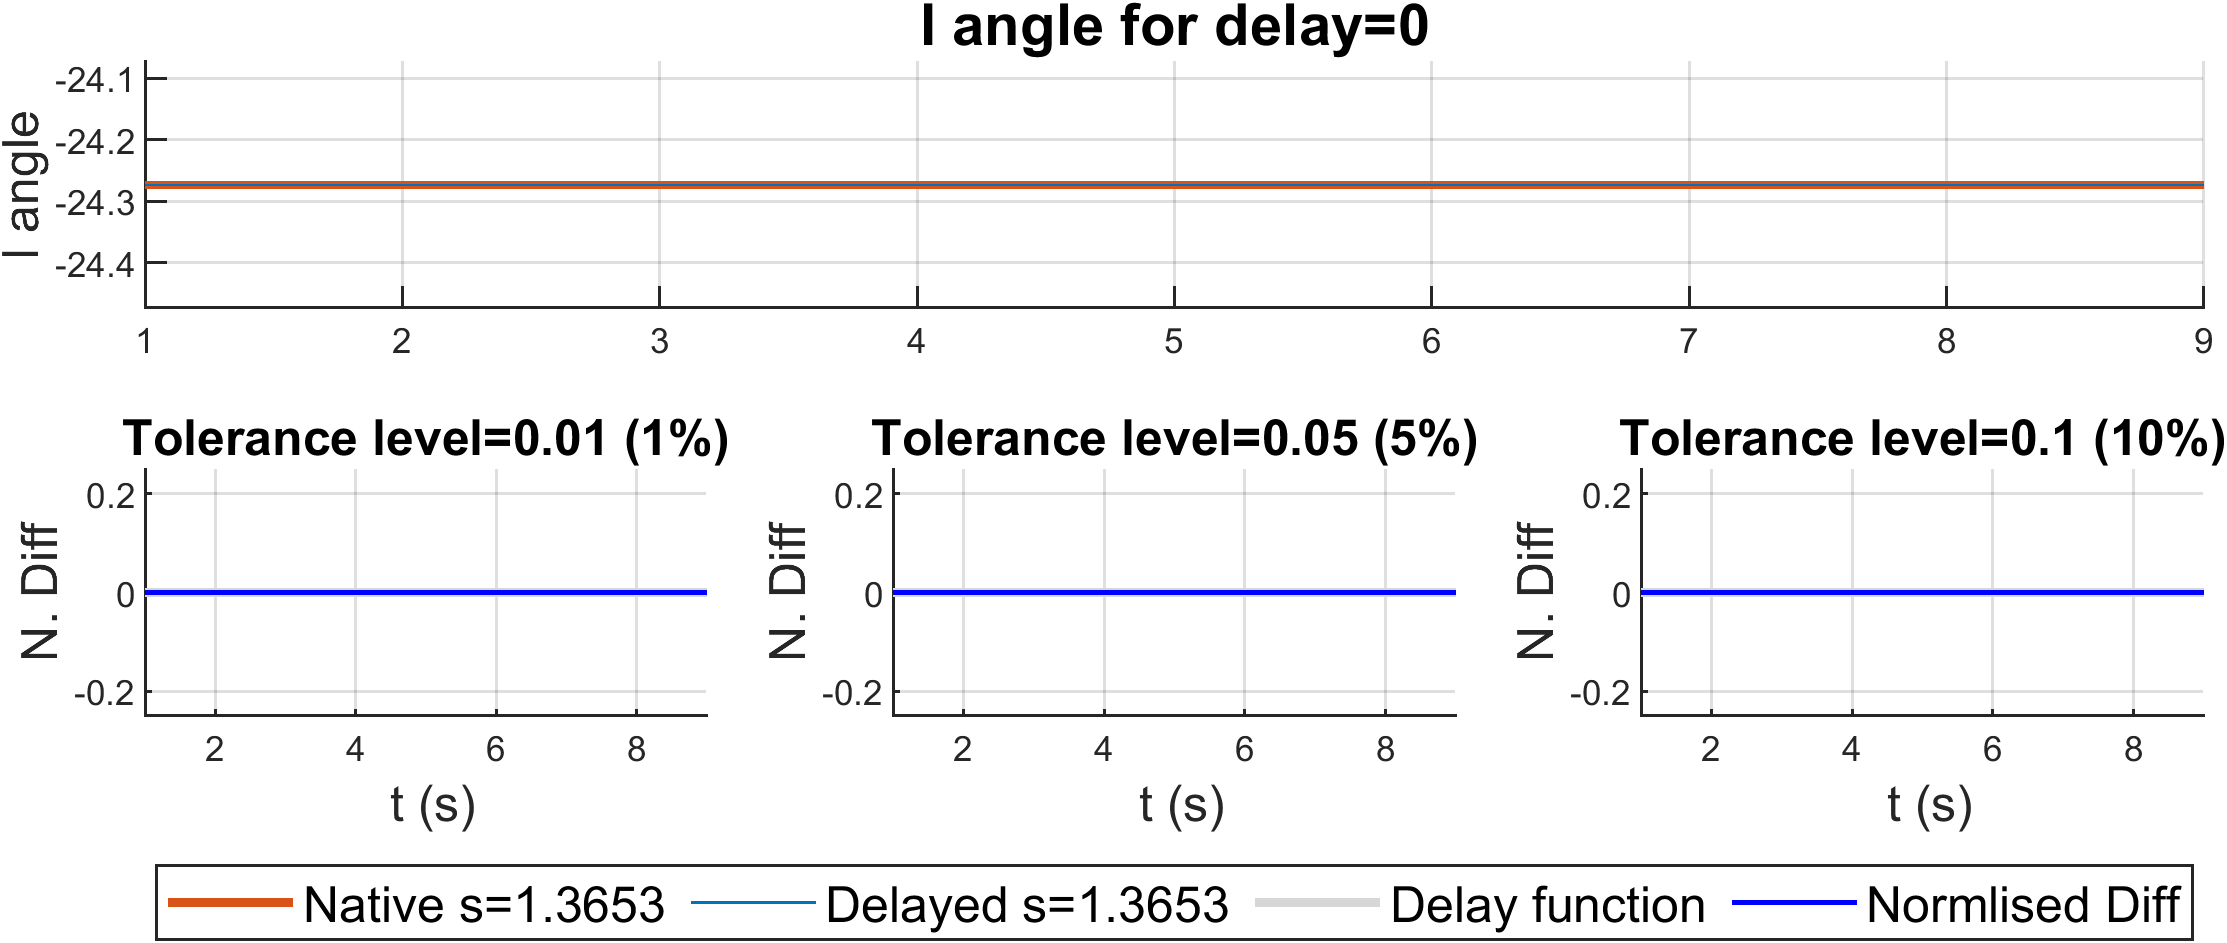
\includegraphics[width=0.95\textwidth]{PMUsim-figures/DelayOf_0/Zero_iAngle.png}}\

     \label{fig:PMUsim_Zero_Angle}
     %\caption{Zero Delay Angle Output (for the Delay Level of Zero)}
  \end{tabular}
 \end{table}

\newpage
\section{Instant Delay Functions}
\newpage \subsection{Delay Level of One}


\begin{table}[]
\caption{Results for Magnitude Output}}\begin{tabular}{c}
   \fbox{     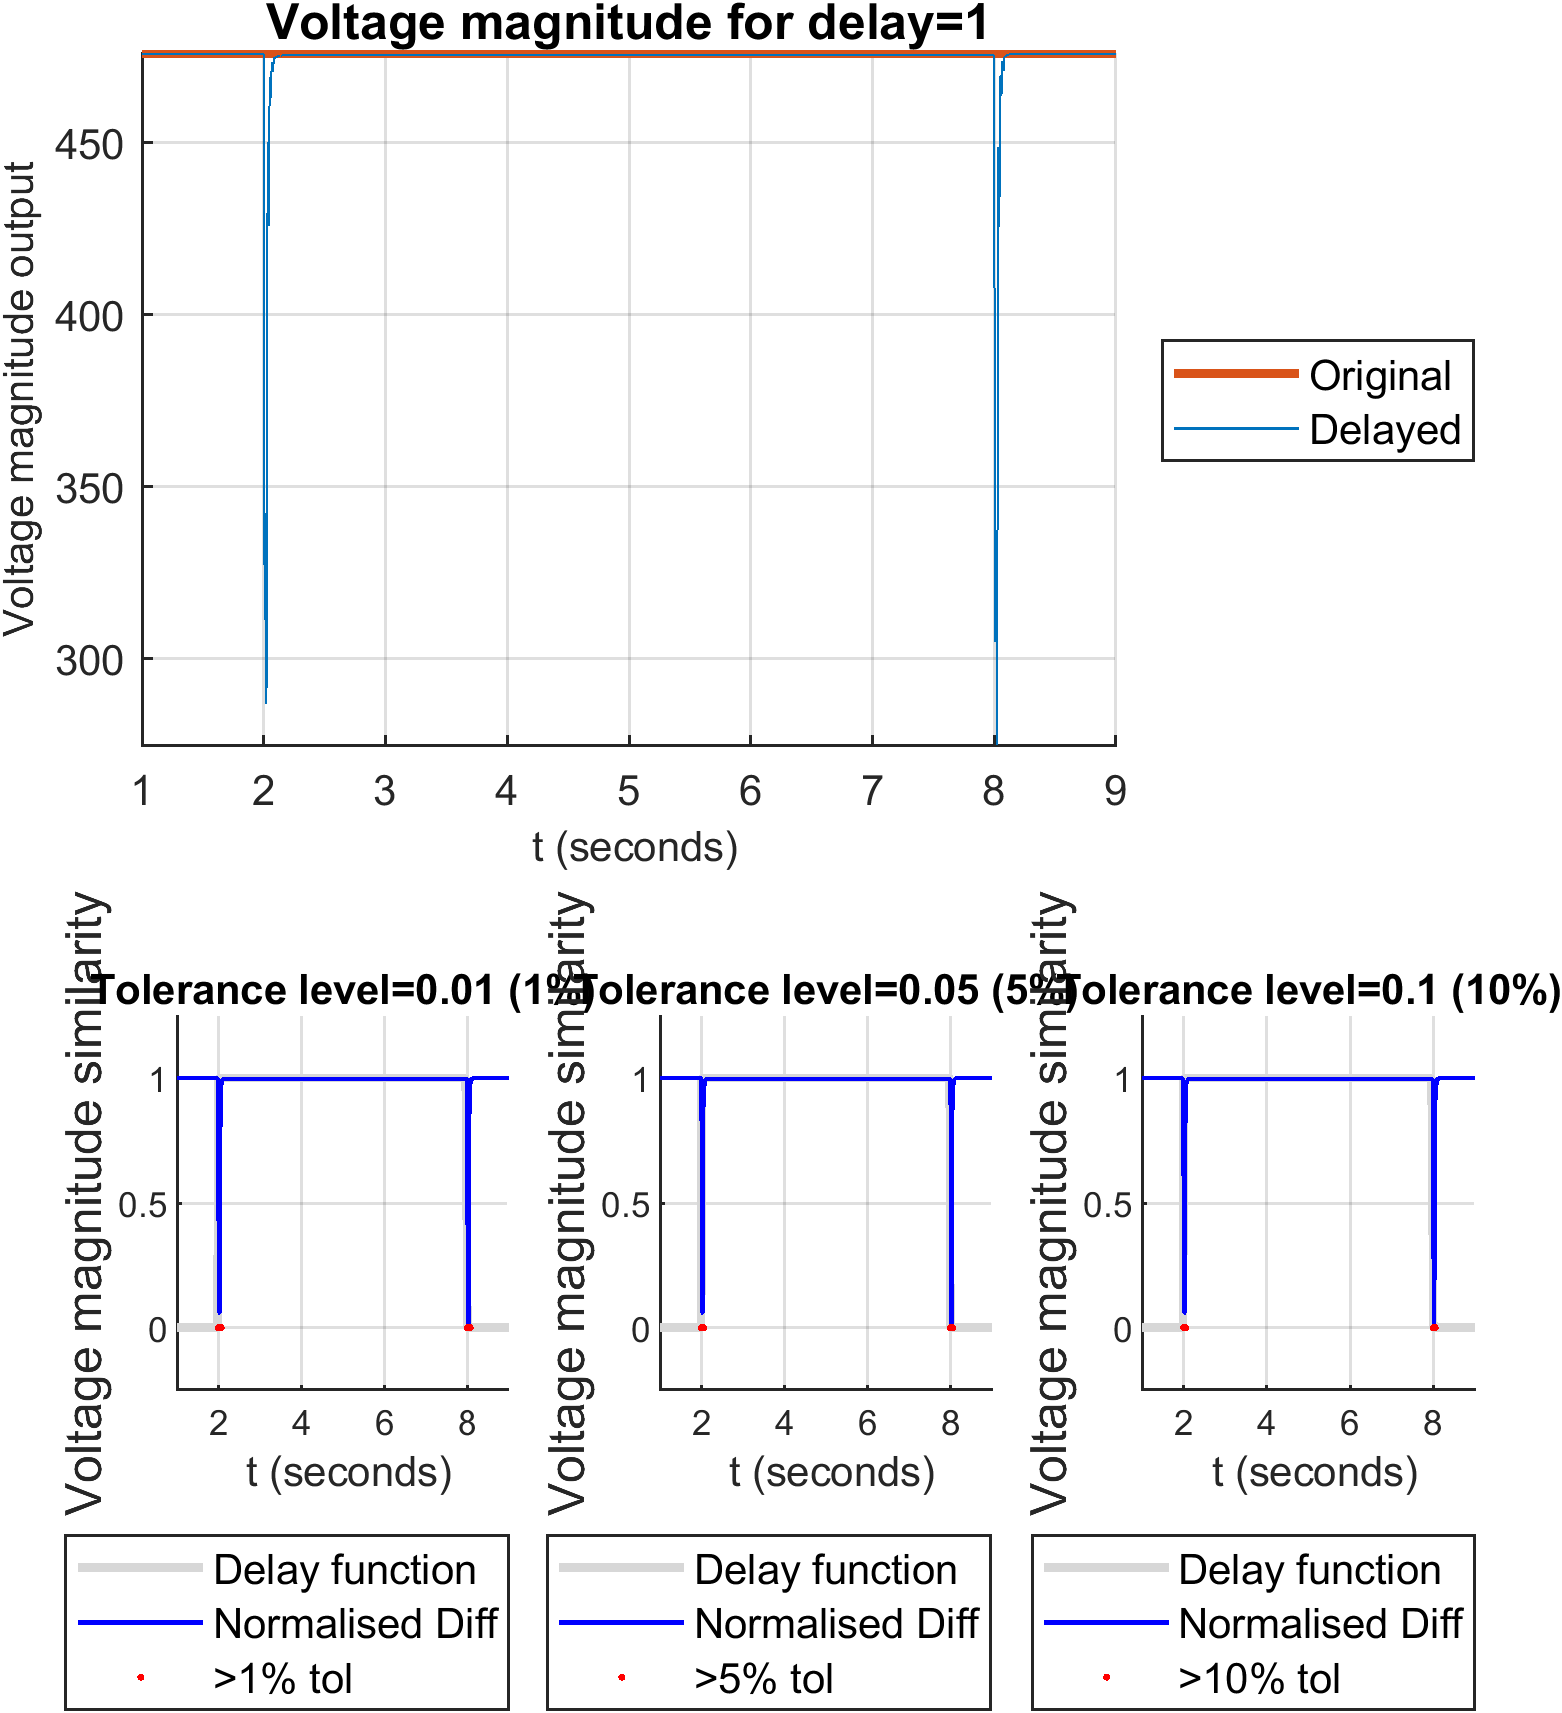
\includegraphics[width=0.95\textwidth]{PMUsim-figures/DelayOf_1/Instant_vMagnitude.png}}\
  
    
   \fbox{  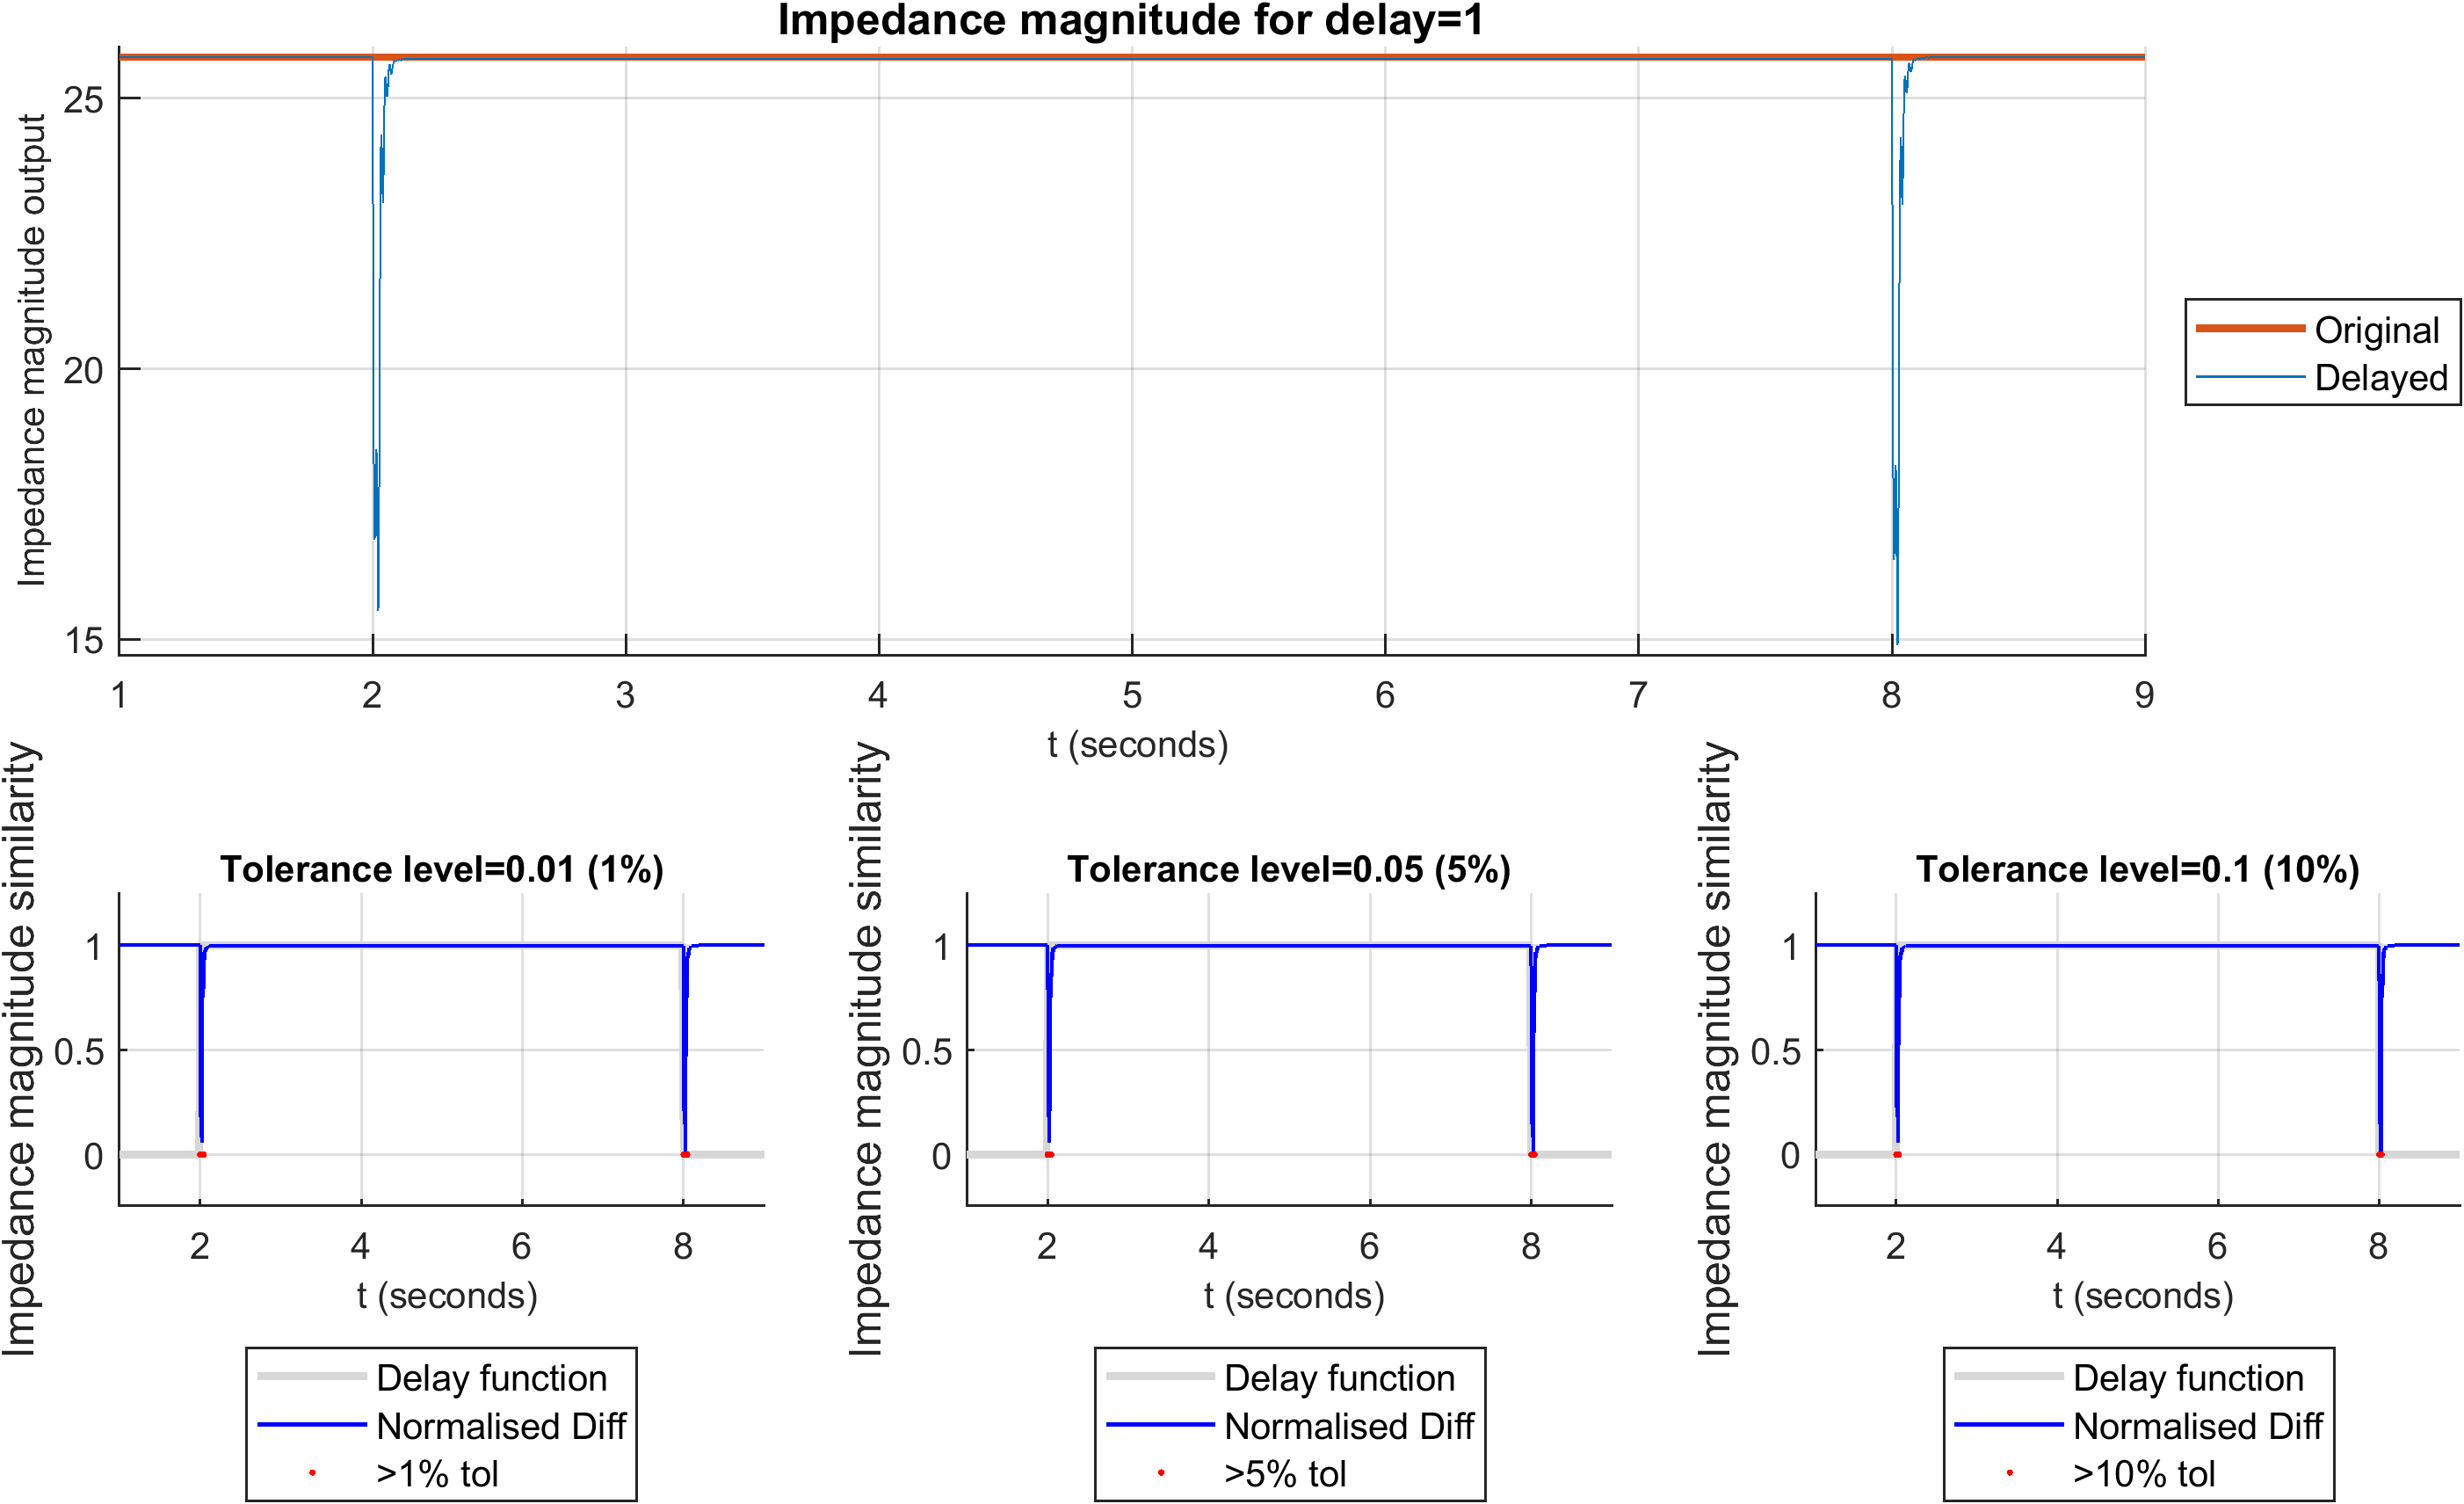
\includegraphics[width=0.95\textwidth]{PMUsim-figures/DelayOf_1/Instant_iMagnitude.png}}\   
 \label{fig:PMUsim_One_Magnitude}
 %\caption{Instant Delay Magnitude Output for the Delay Level of One}
  \end{tabular}
 \end{table}

\newpage

\begin{table}[]
\caption{Results for Frequency Output}
  
   \fbox{  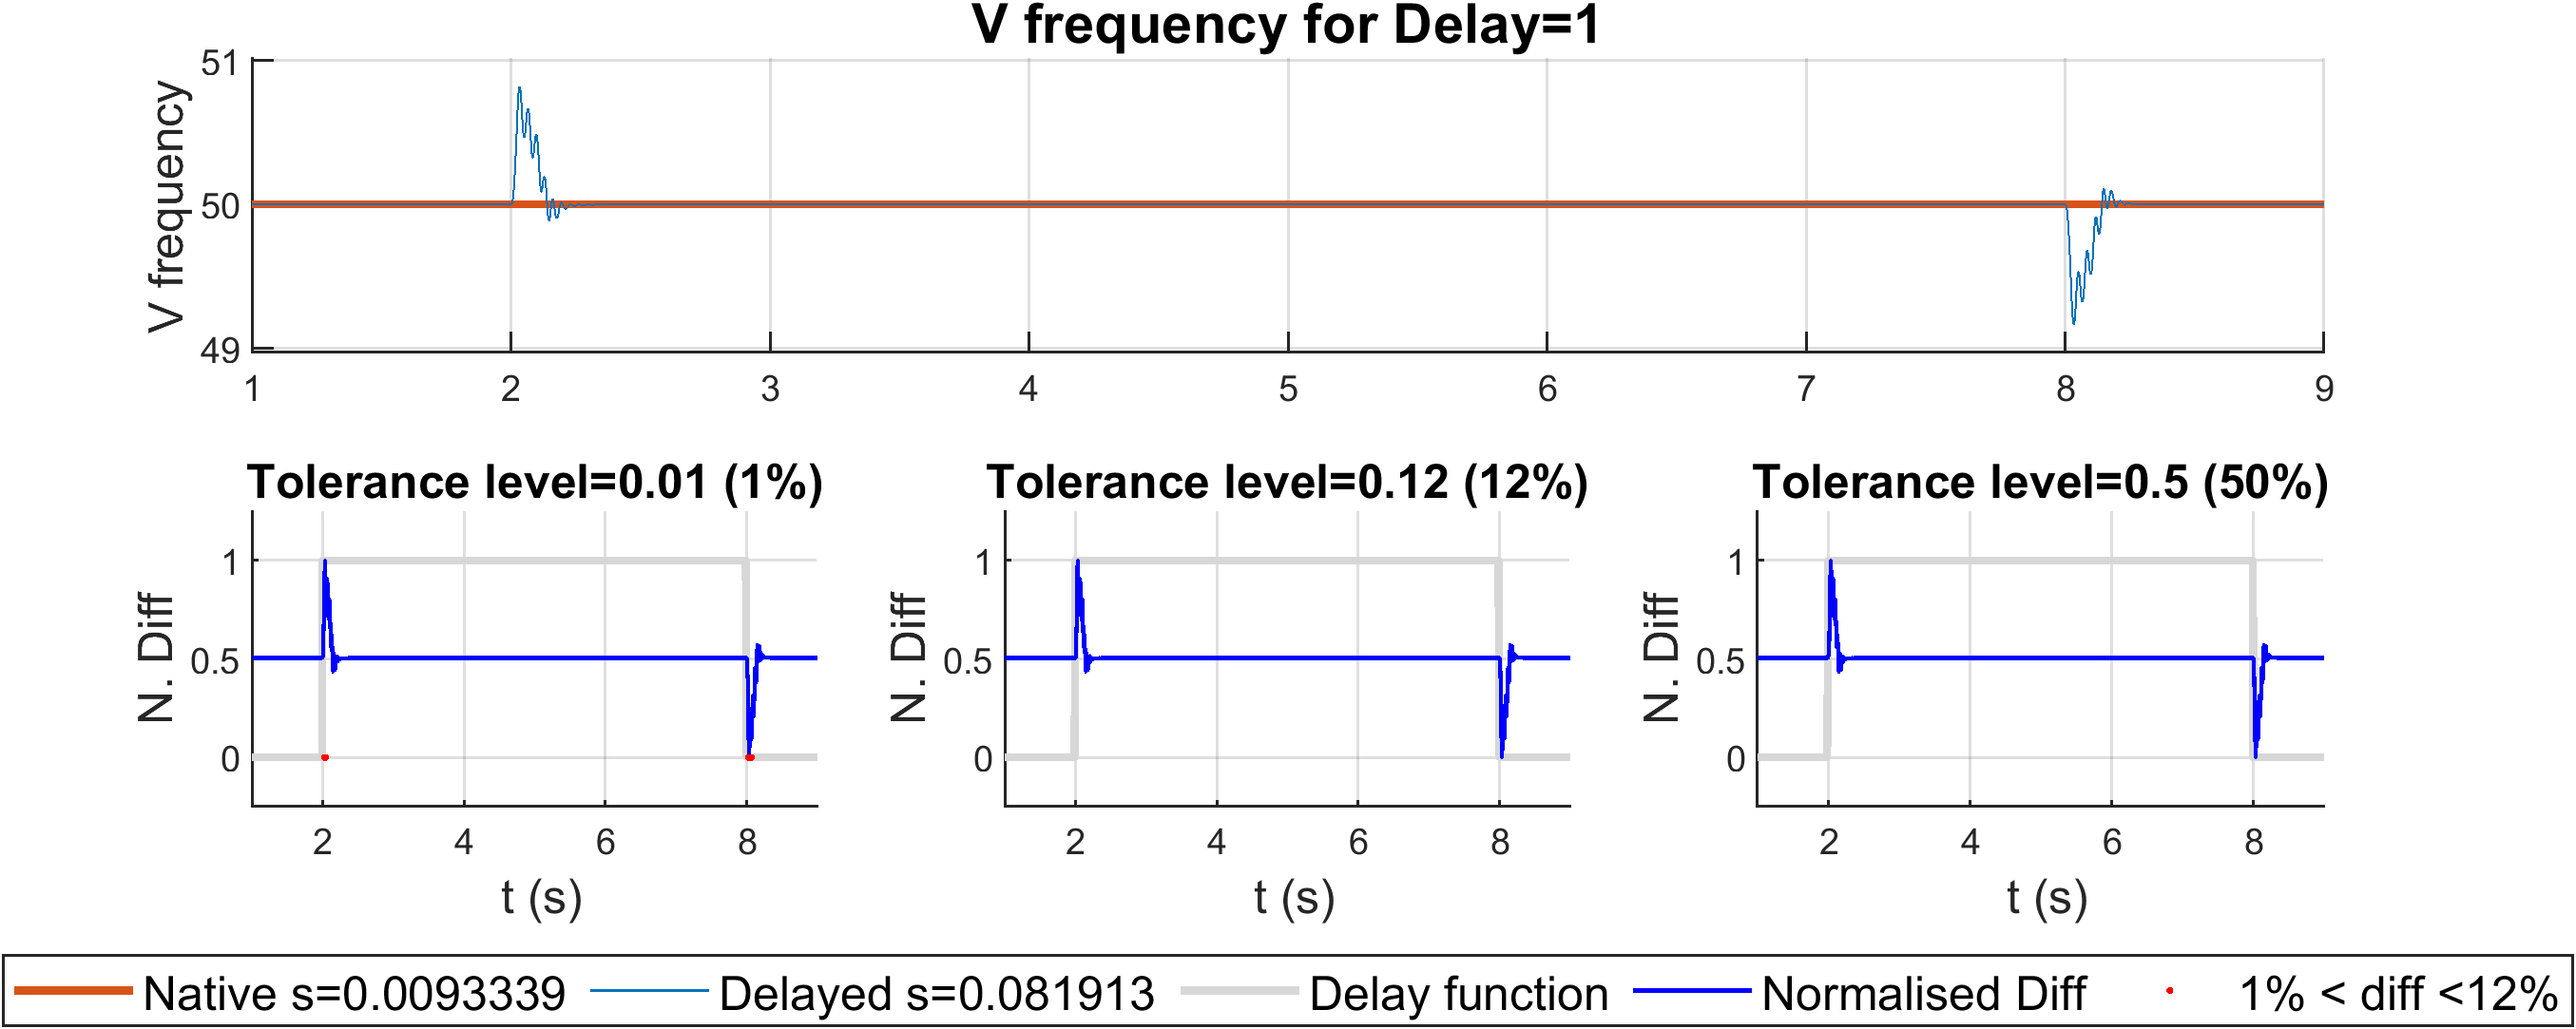
\includegraphics[width=0.95\textwidth]{PMUsim-figures/DelayOf_1/Instant_vFrequency.png}}\
  
    
   \fbox{  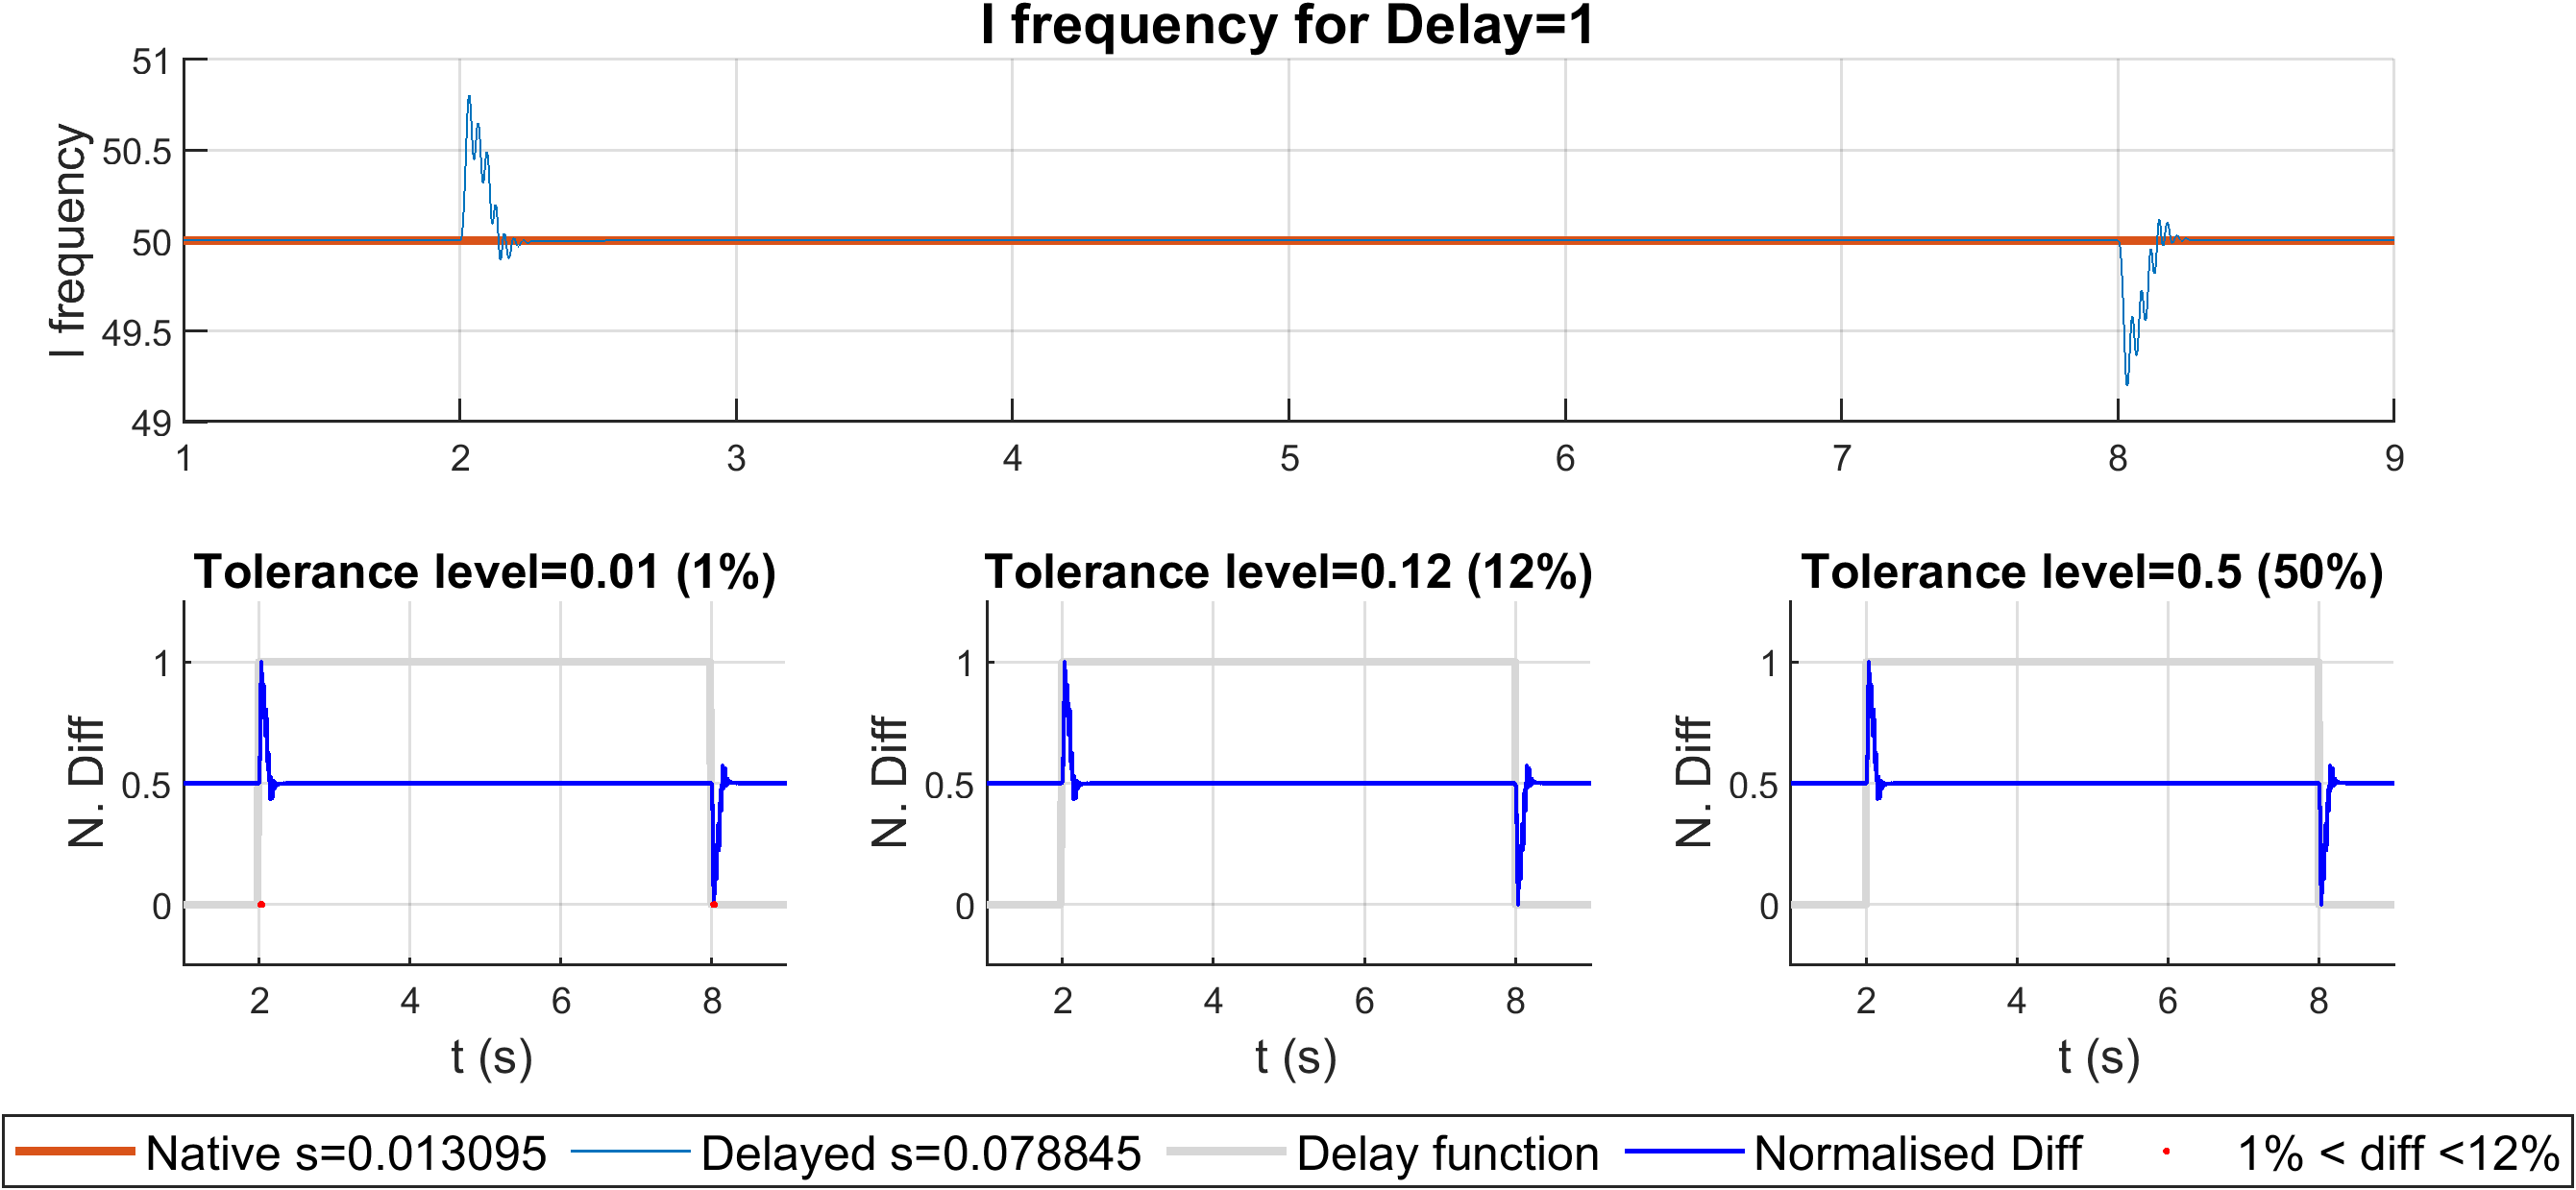
\includegraphics[width=0.95\textwidth]{PMUsim-figures/DelayOf_1/Instant_iFrequency.png}}\ 
 \label{fig:PMUsim_One_Frequency}
 %\caption{Instant Delay Frequency Output for the Delay Level of One}
  \end{tabular}
 \end{table}



\newpage 

\begin{table}[]
\caption{Results for Angle Output}
   \fbox{    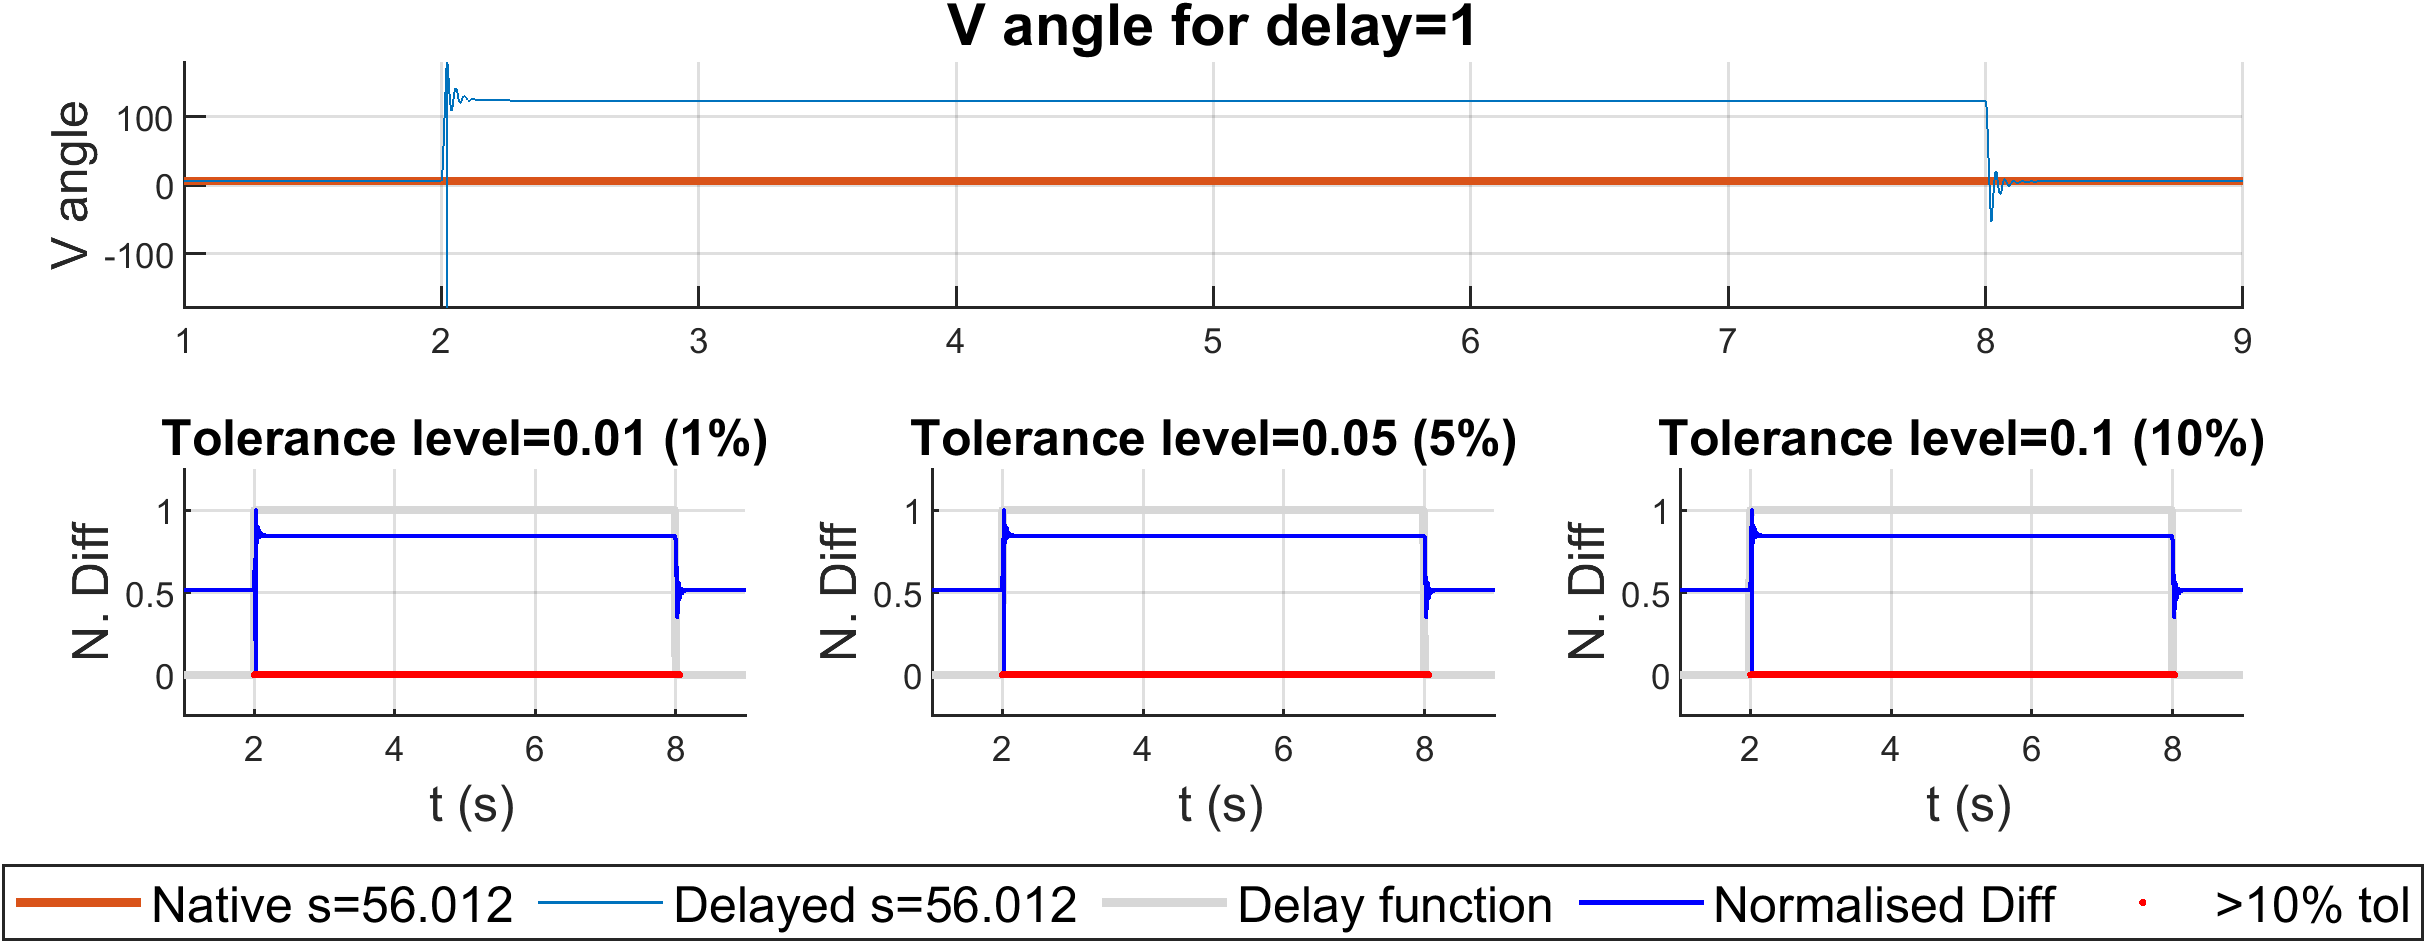
\includegraphics[width=0.95\textwidth]{PMUsim-figures/DelayOf_1/Instant_vAngle.png}}\
  
    
   \fbox{  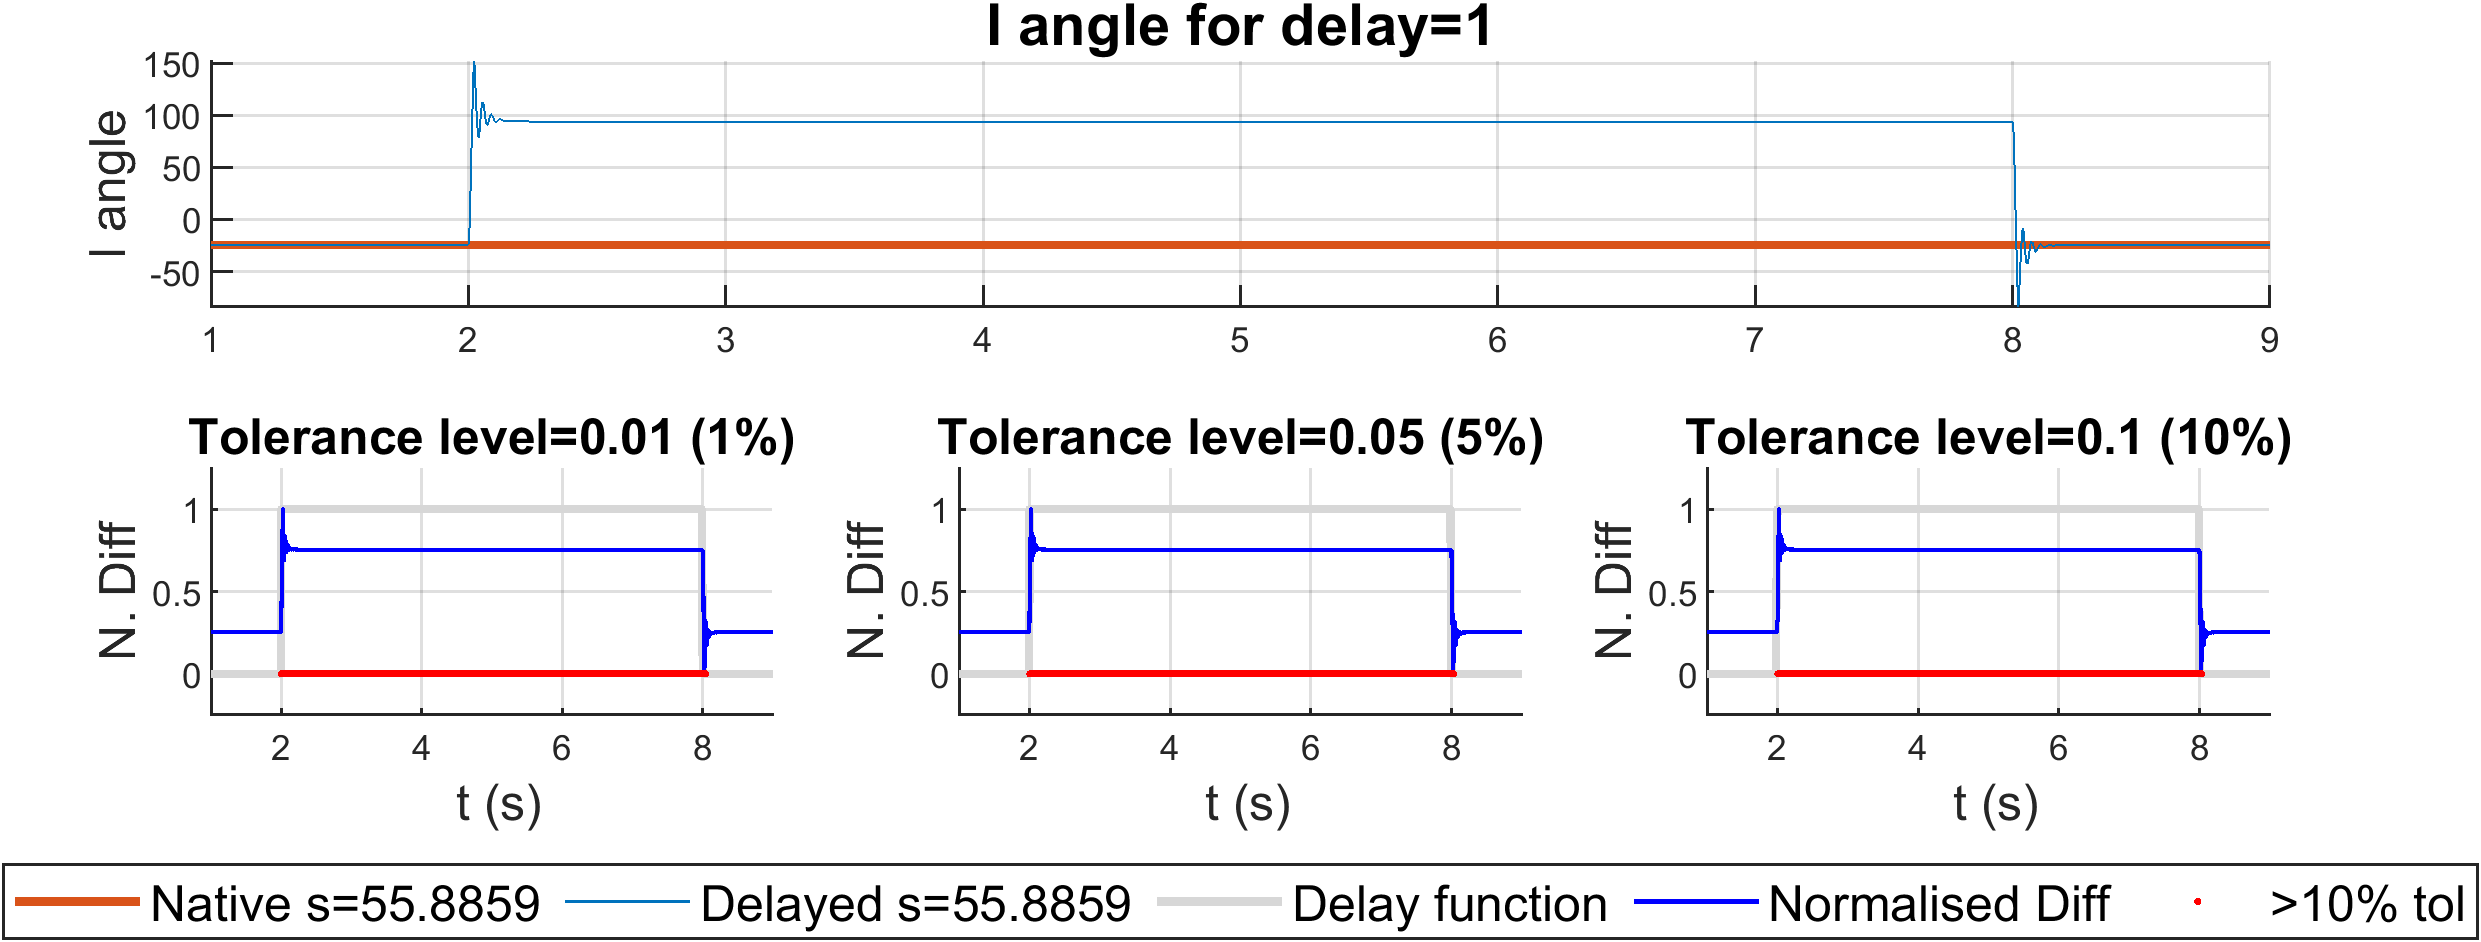
\includegraphics[width=0.95\textwidth]{PMUsim-figures/DelayOf_1/Instant_iAngle.png}}\
   \label{fig:PMUsim_One_Angle}
 %\caption{Instant Delay Angle Output for the Delay Level of One}
  \end{tabular}
 \end{table}

\newpage 

\subsection{Delay Level of Two}


\begin{table}[]
\caption{Results for Magnitude Output}
   \fbox{     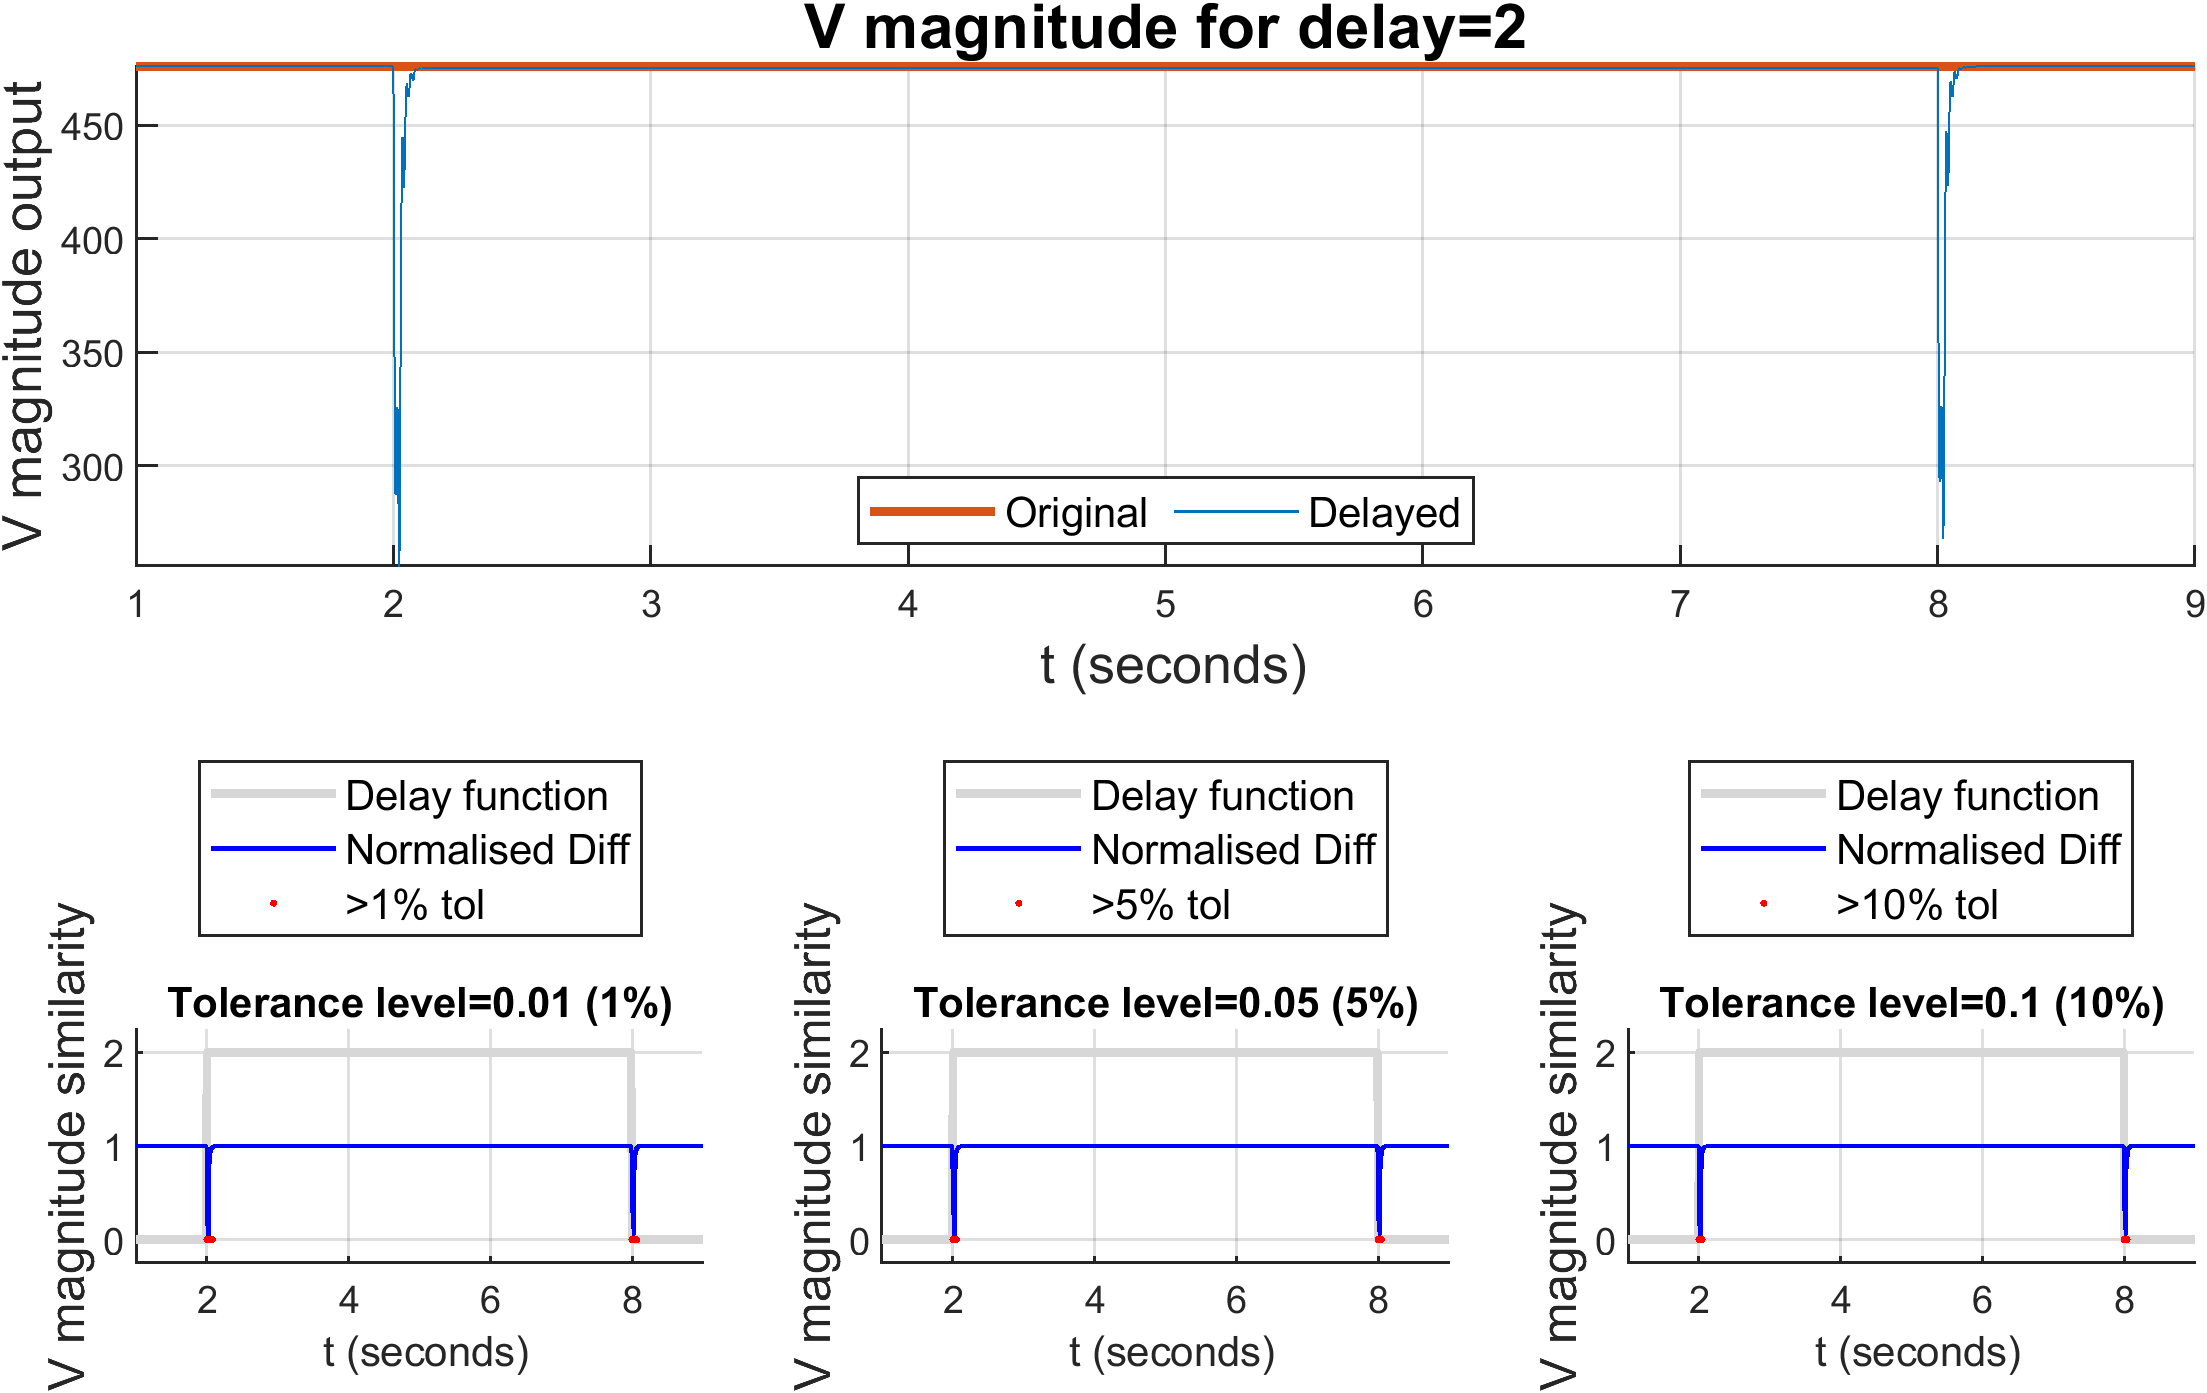
\includegraphics[width=0.95\textwidth]{PMUsim-figures/DelayOf_2/Instant_vMagnitude.png}}\
  
    
   \fbox{   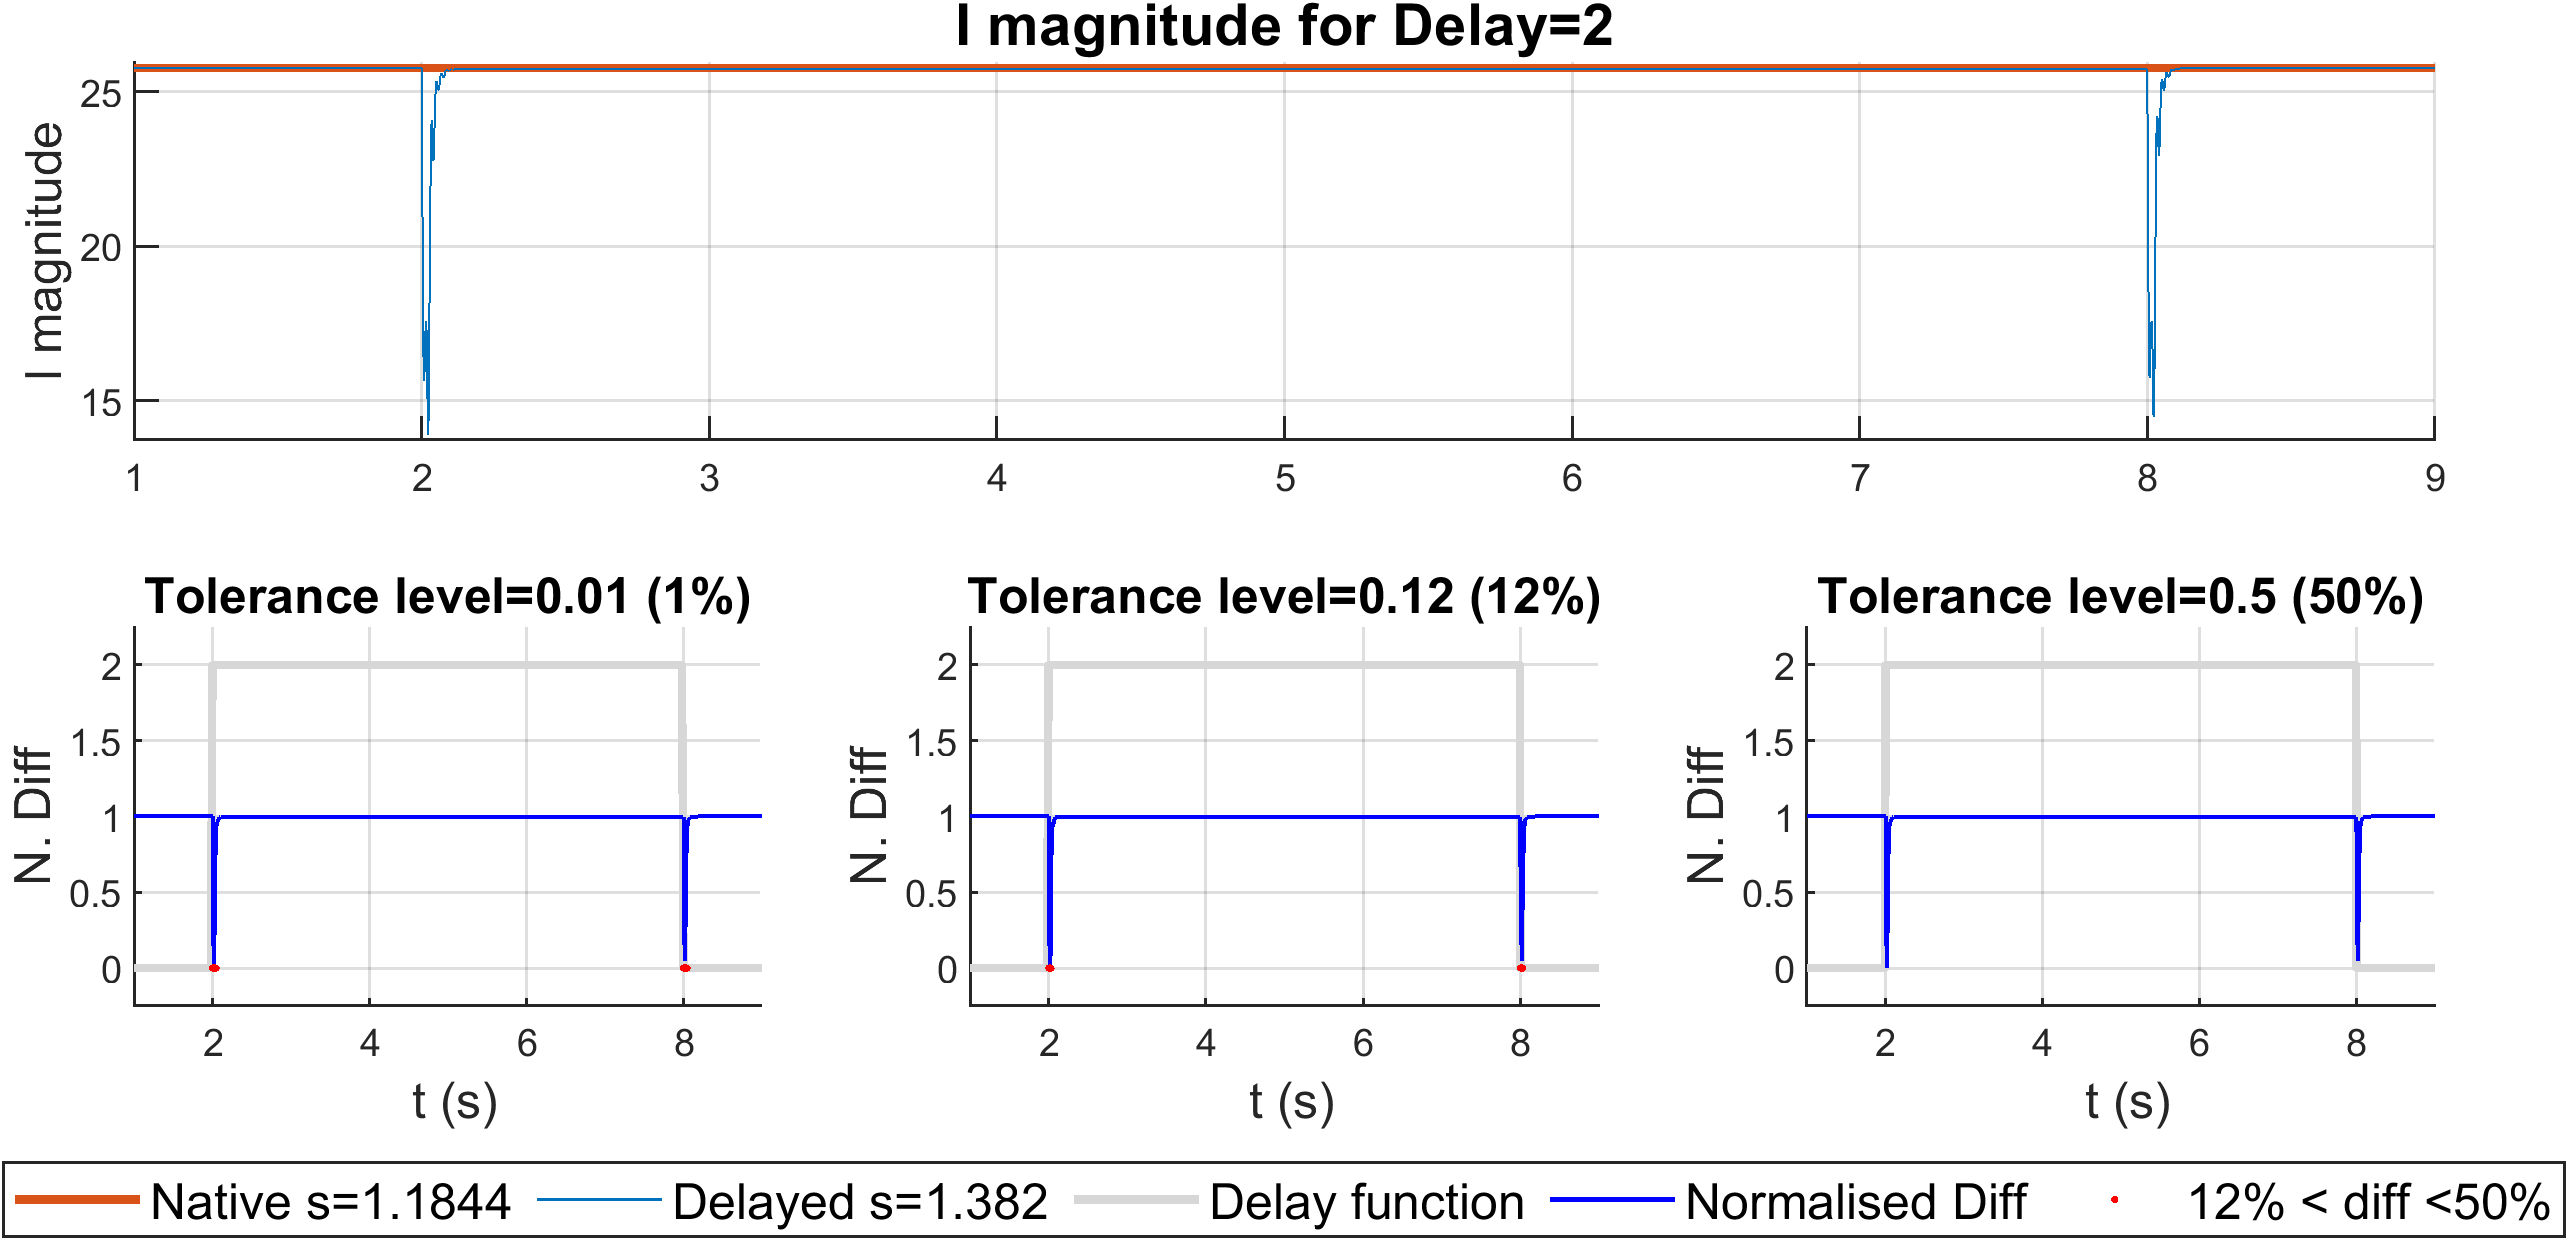
\includegraphics[width=0.95\textwidth]{PMUsim-figures/DelayOf_2/Instant_iMagnitude.png}}\
 \label{fig:PMUsim_Two_Magnitude}
 %\caption{Instant Delay Magnitude Output for the Delay Level of Two}
  \end{tabular}
 \end{table}

\newpage 

\begin{table}[]
\caption{Results for Frequency Output}
   \fbox{     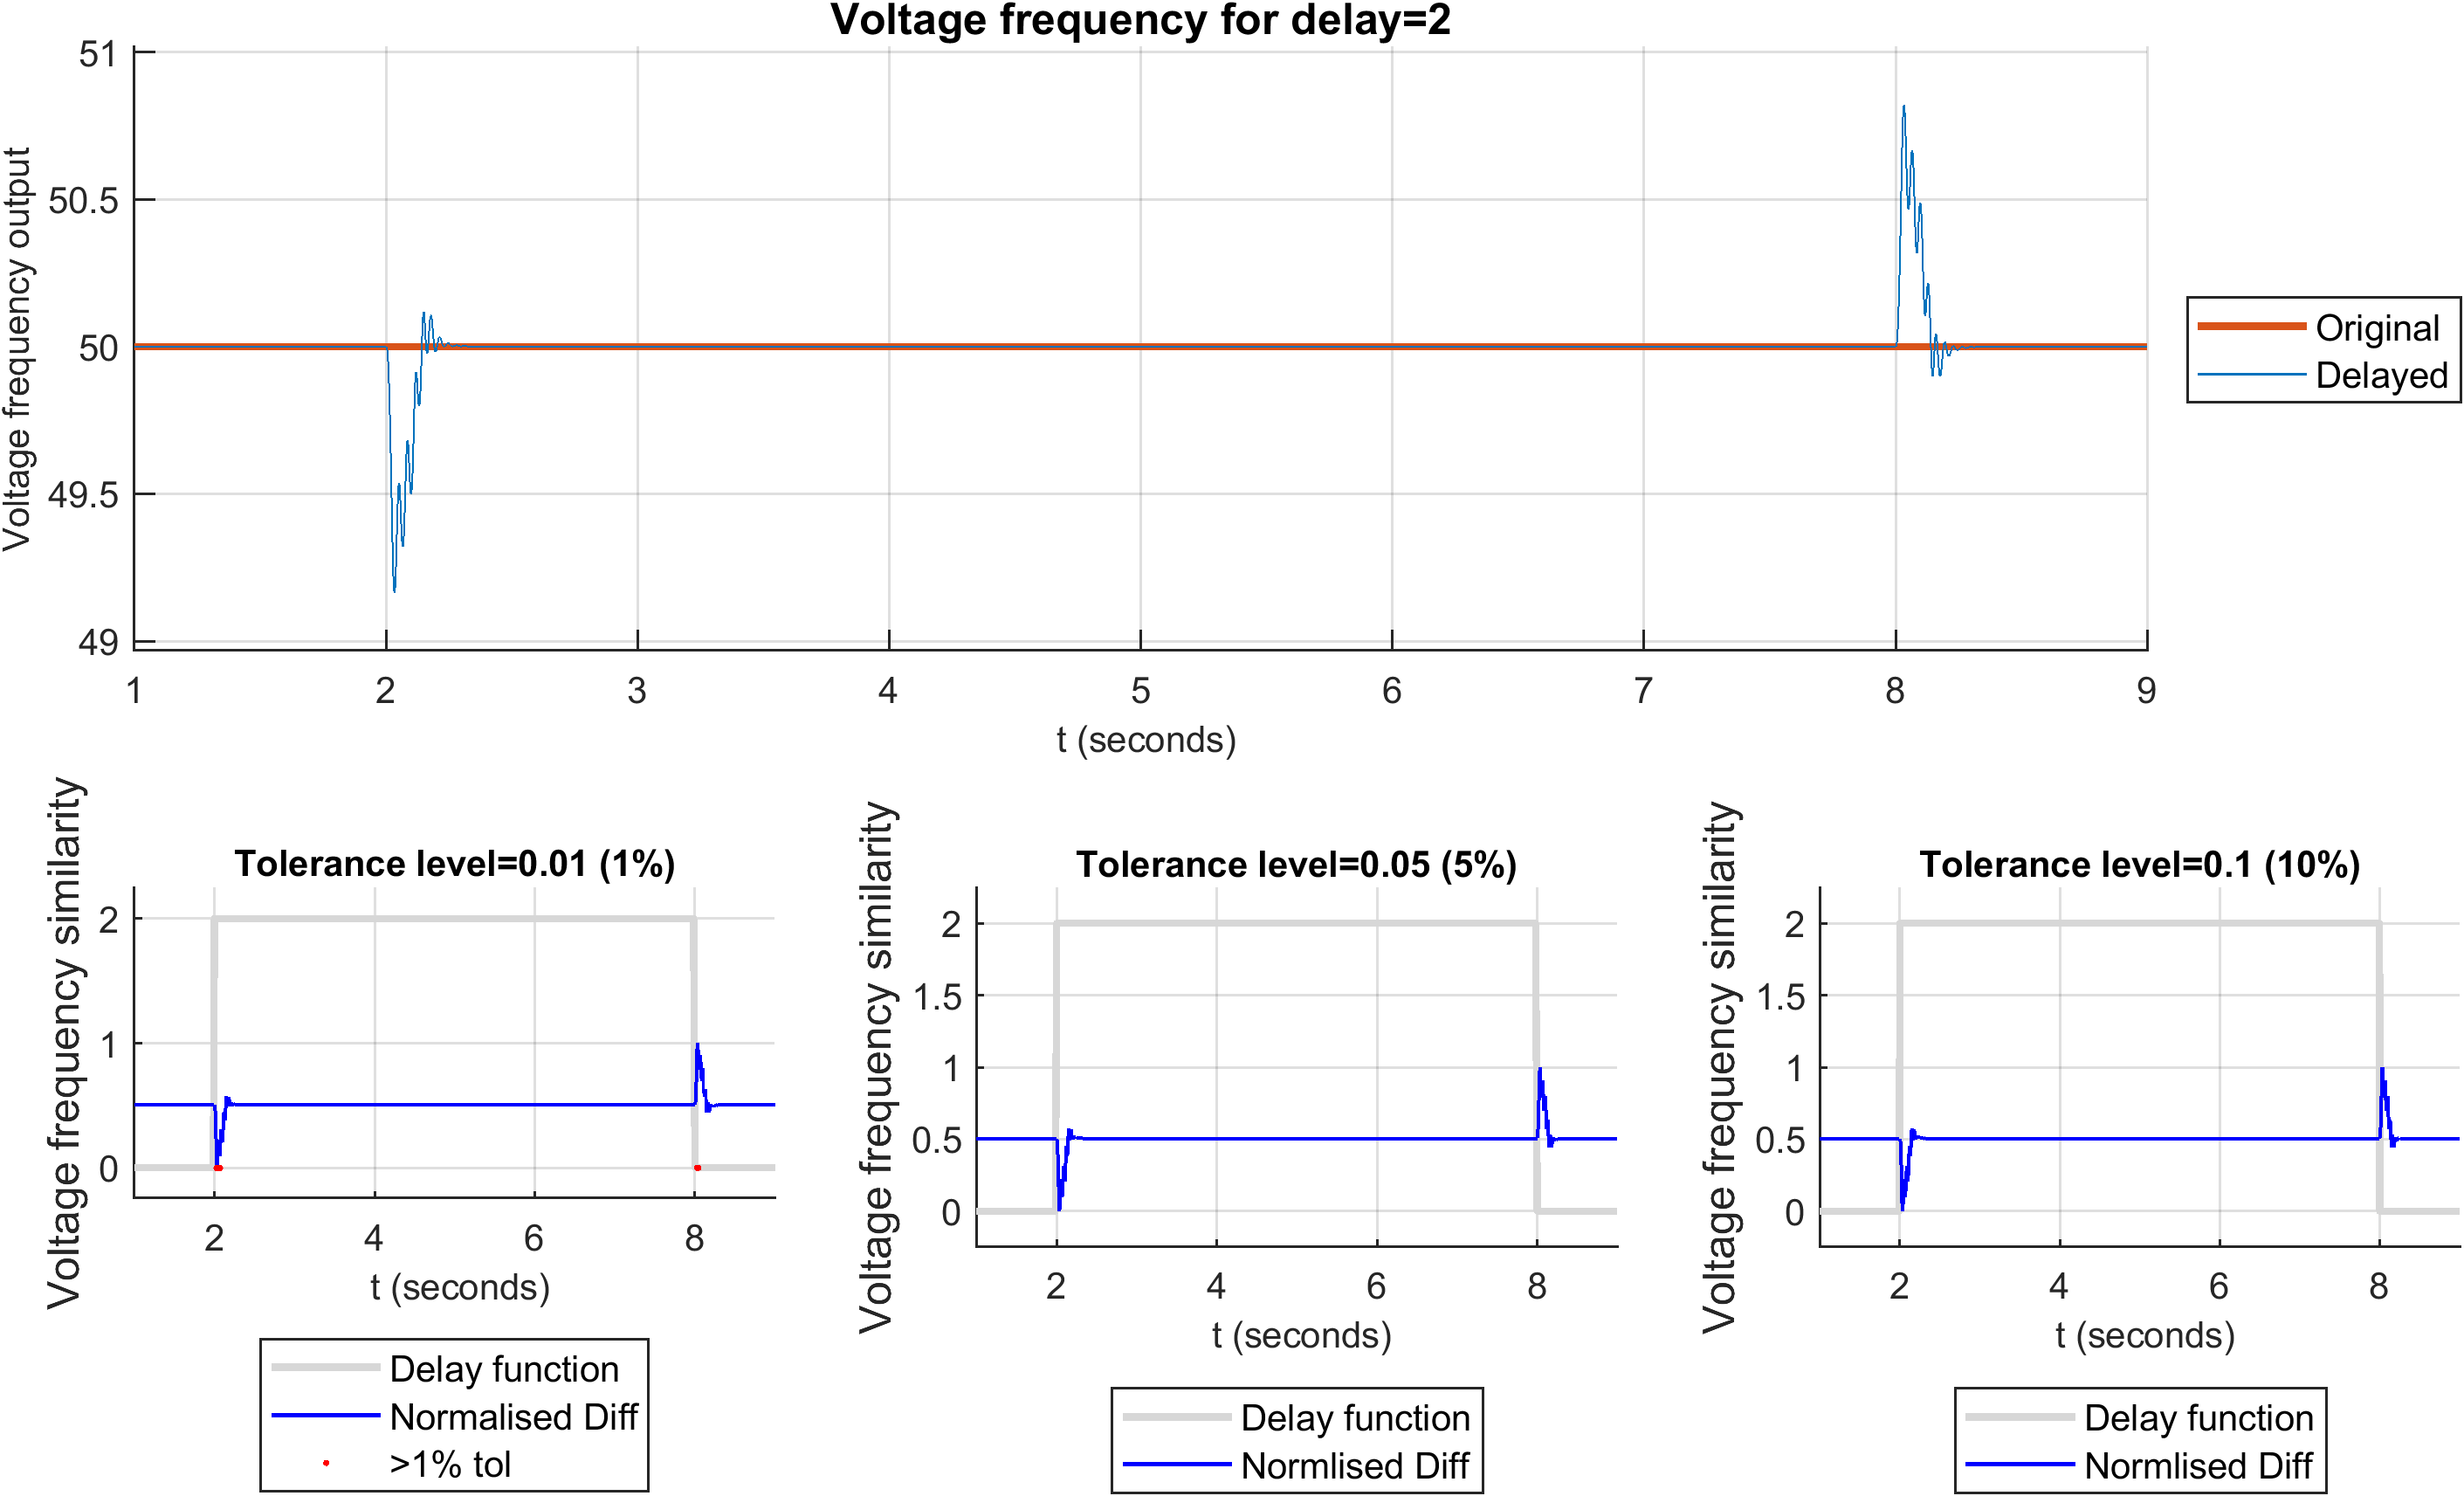
\includegraphics[width=0.95\textwidth]{PMUsim-figures/DelayOf_2/Instant_vFrequency.png}}\
  
    
   \fbox{   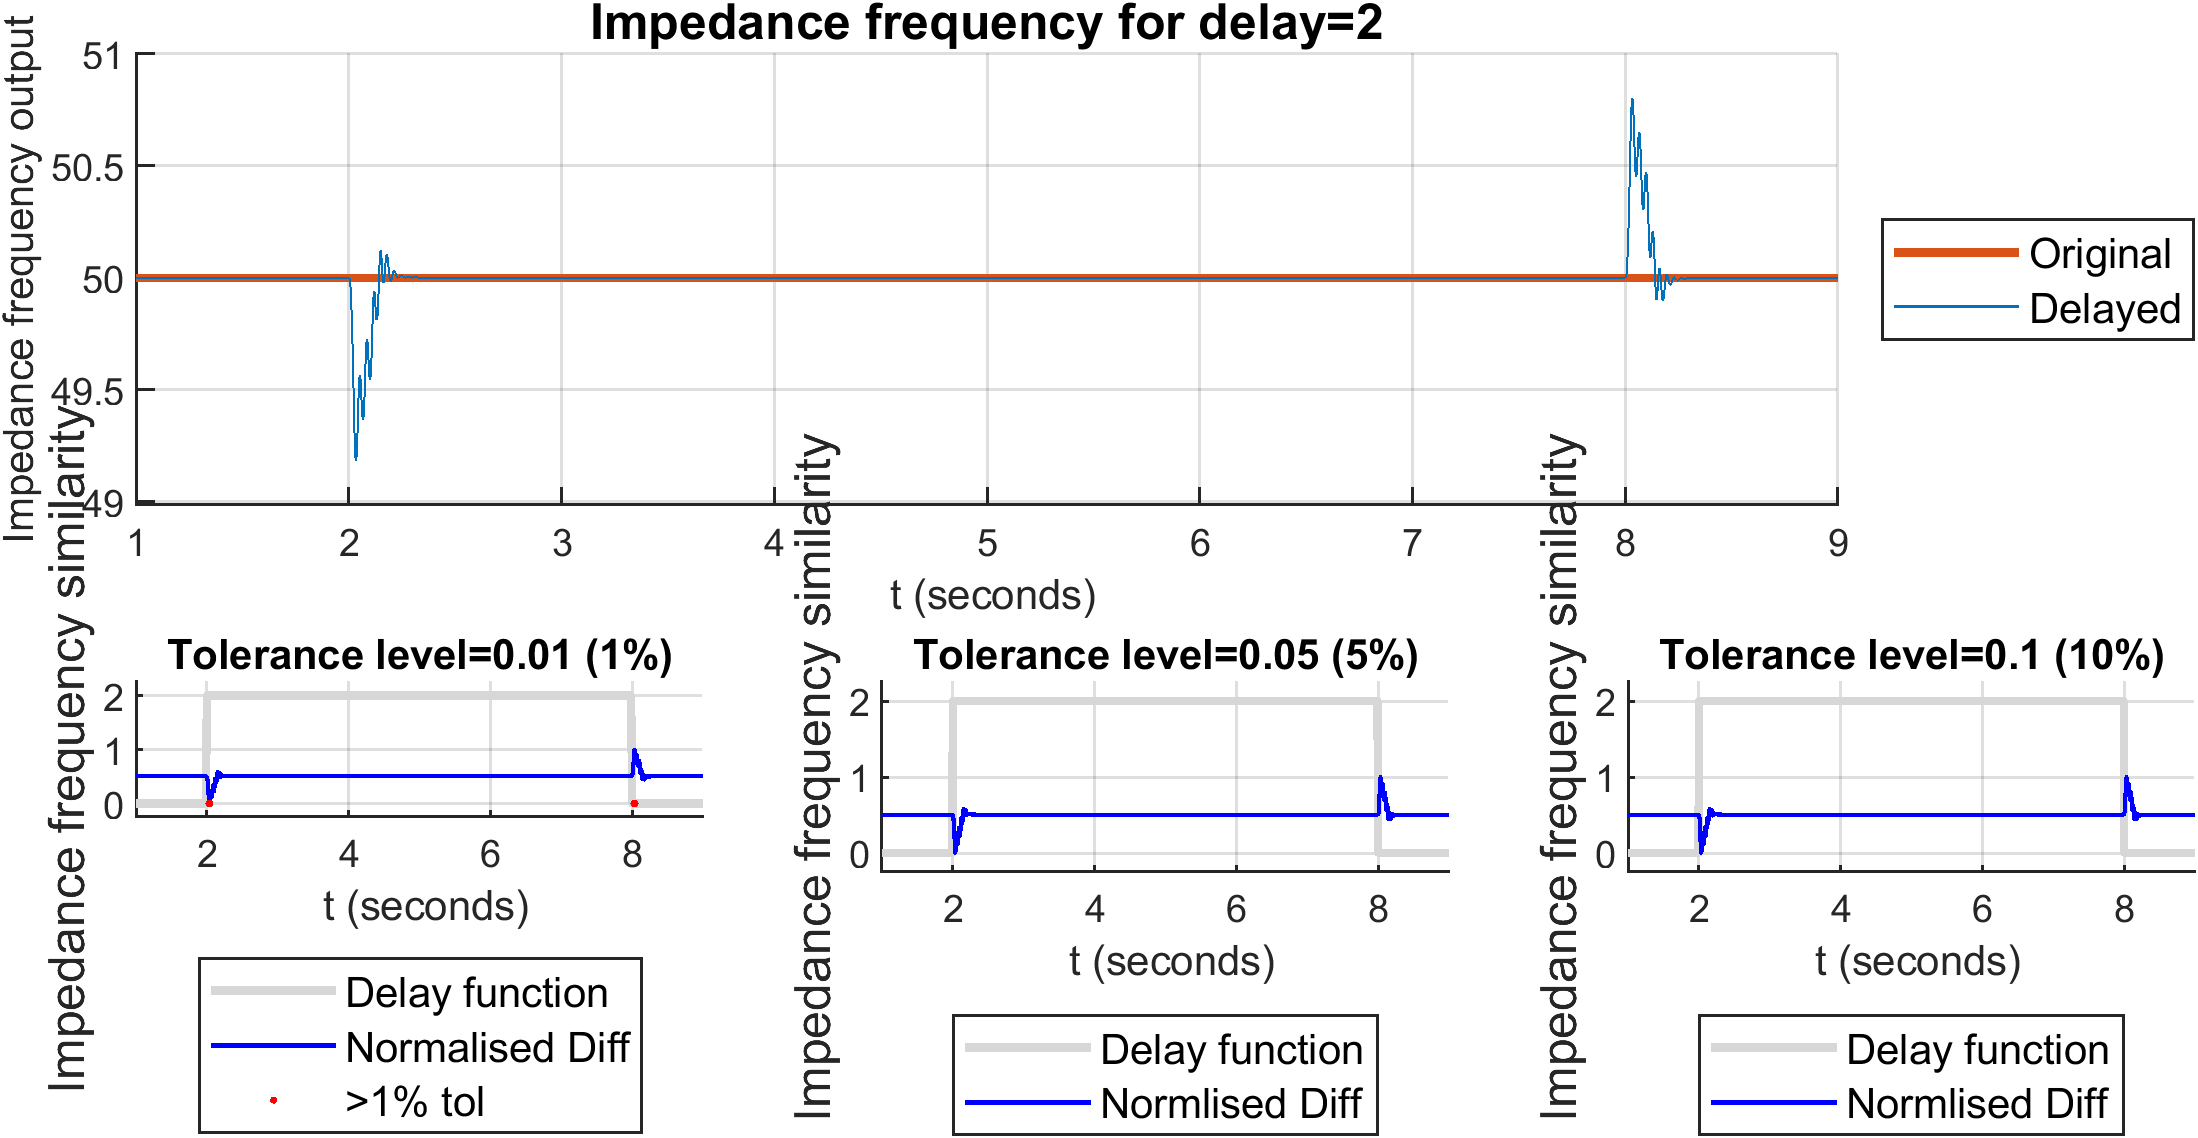
\includegraphics[width=0.95\textwidth]{PMUsim-figures/DelayOf_2/Instant_iFrequency.png}}\   
 \label{fig:PMUsim_Two_Frequency}
 %\caption{Instant Delay Frequency Output for the Delay Level of Two}
  \end{tabular}
 \end{table}


\newpage 
\begin{table}[]
\caption{Results for Angle Output}
   \fbox{     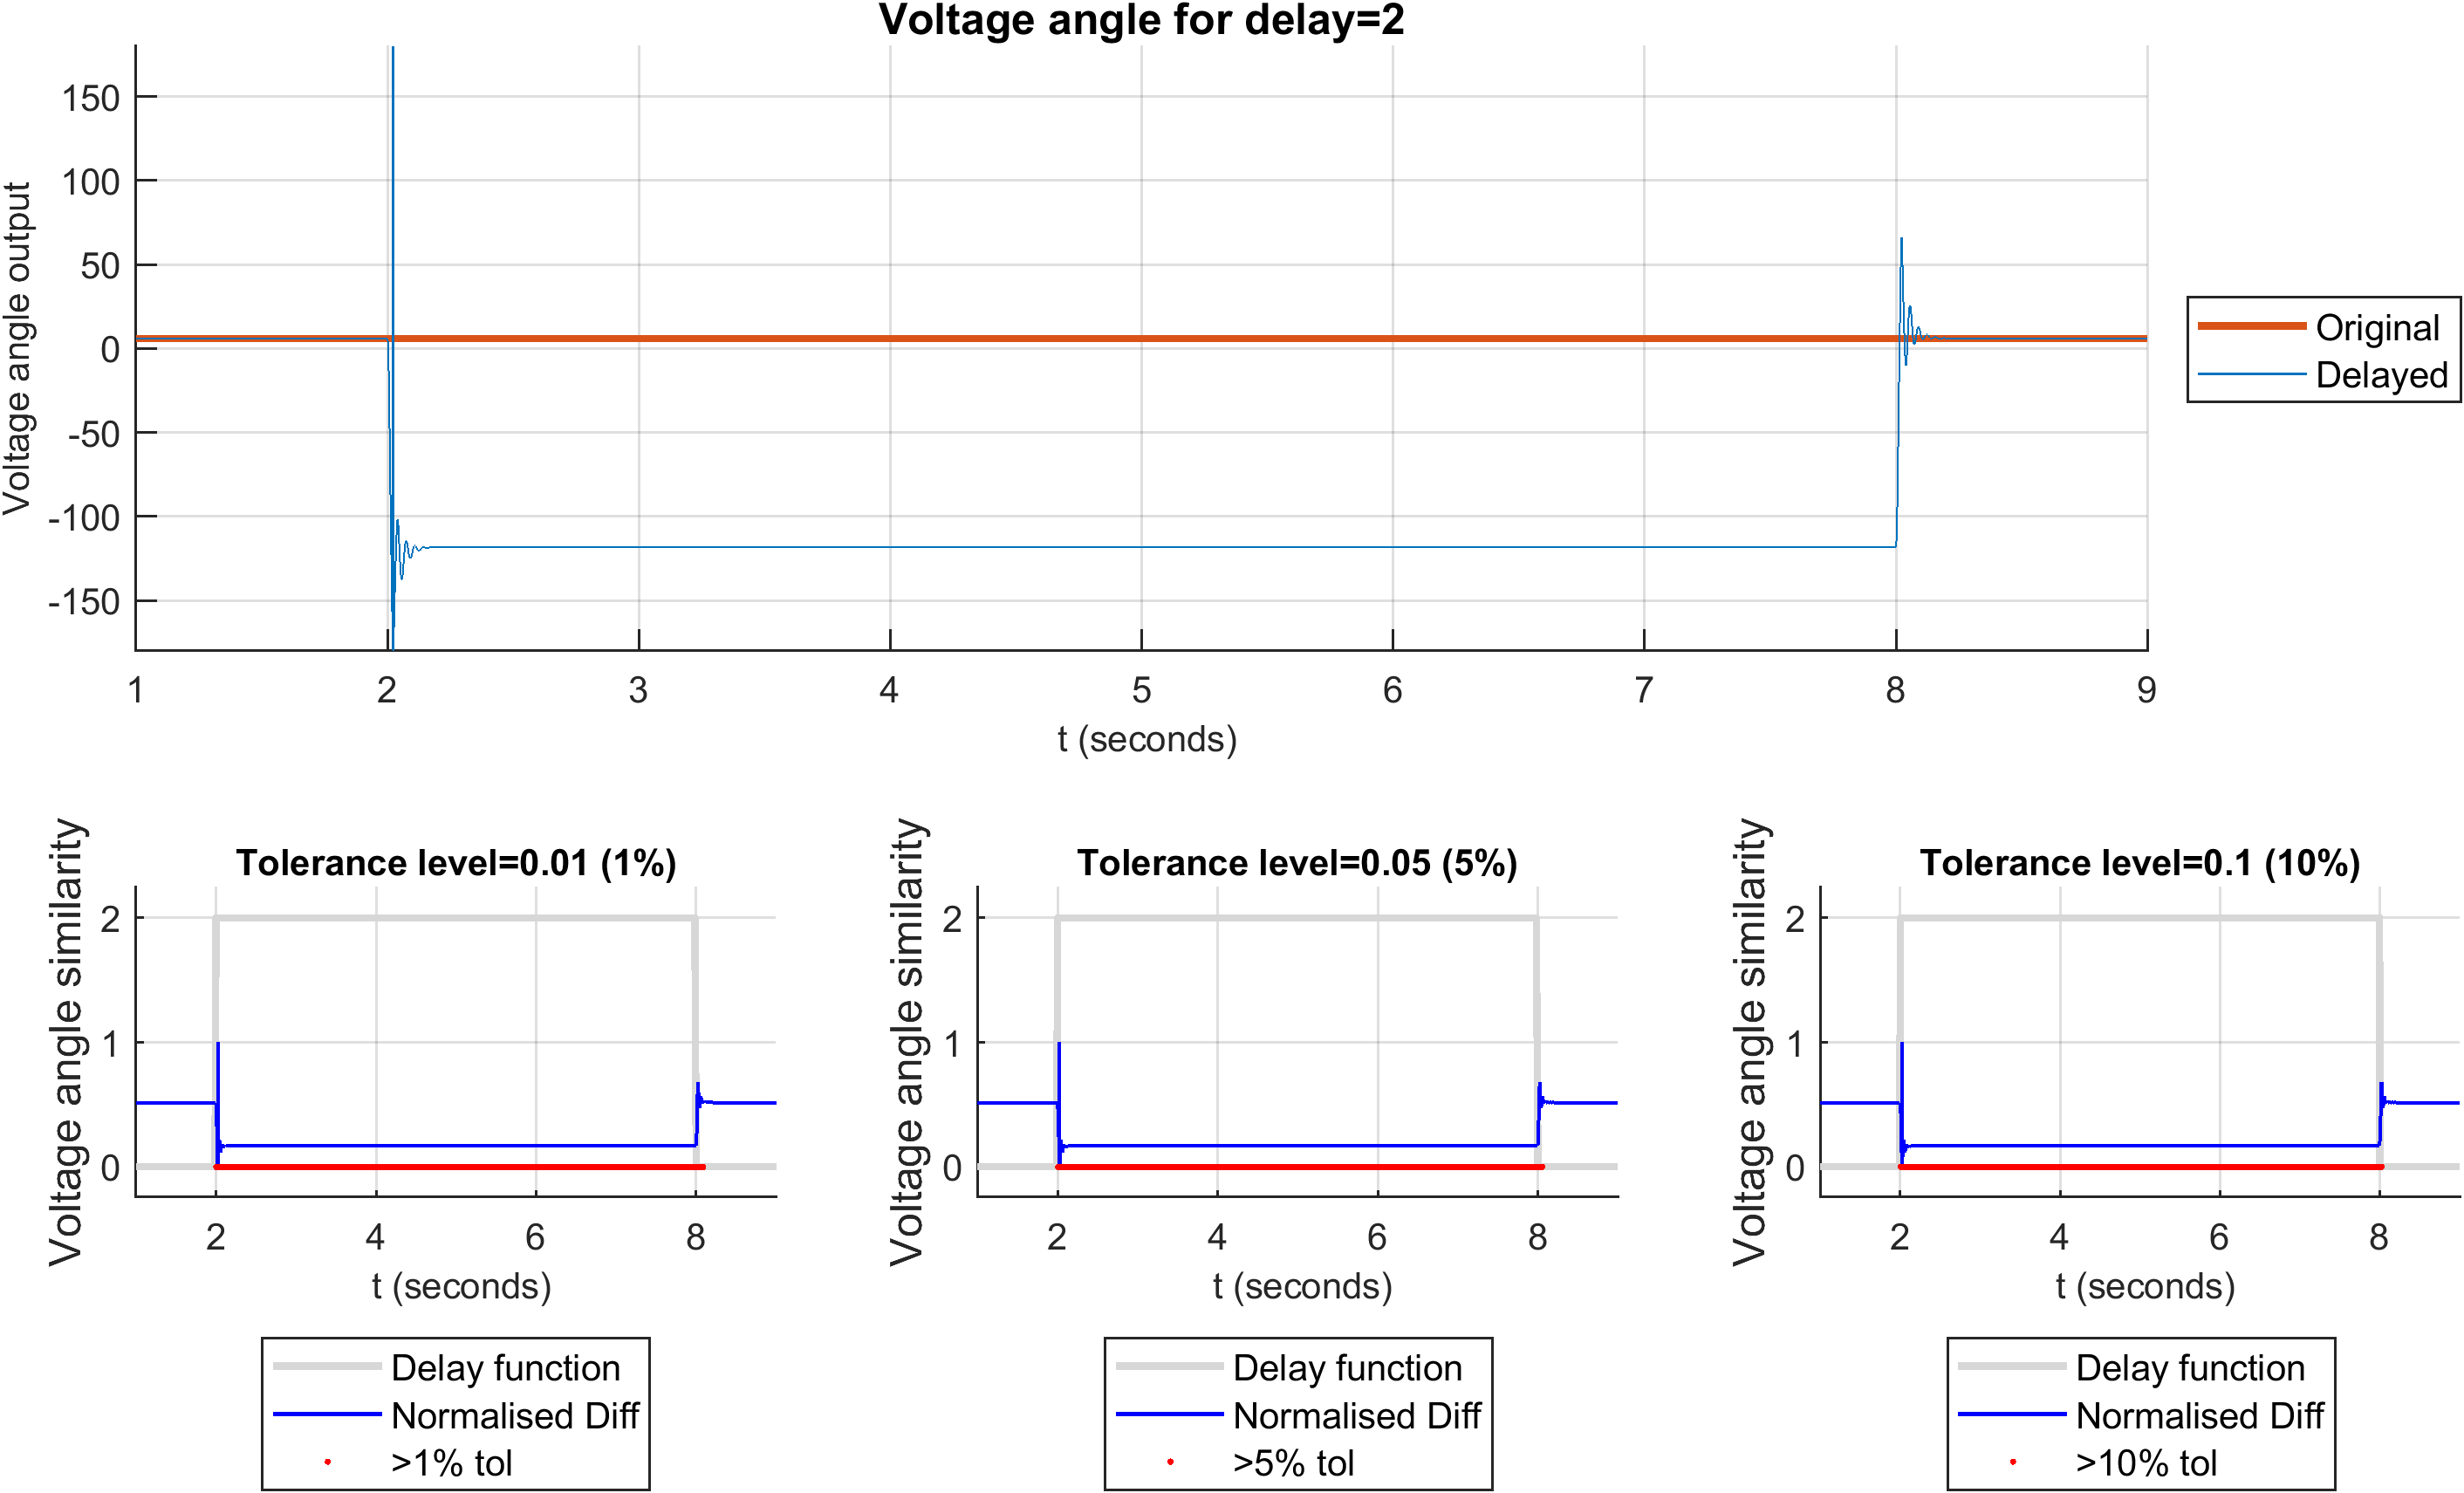
\includegraphics[width=0.95\textwidth]{PMUsim-figures/DelayOf_2/Instant_vAngle.png}}\
  \\ 
   \fbox{   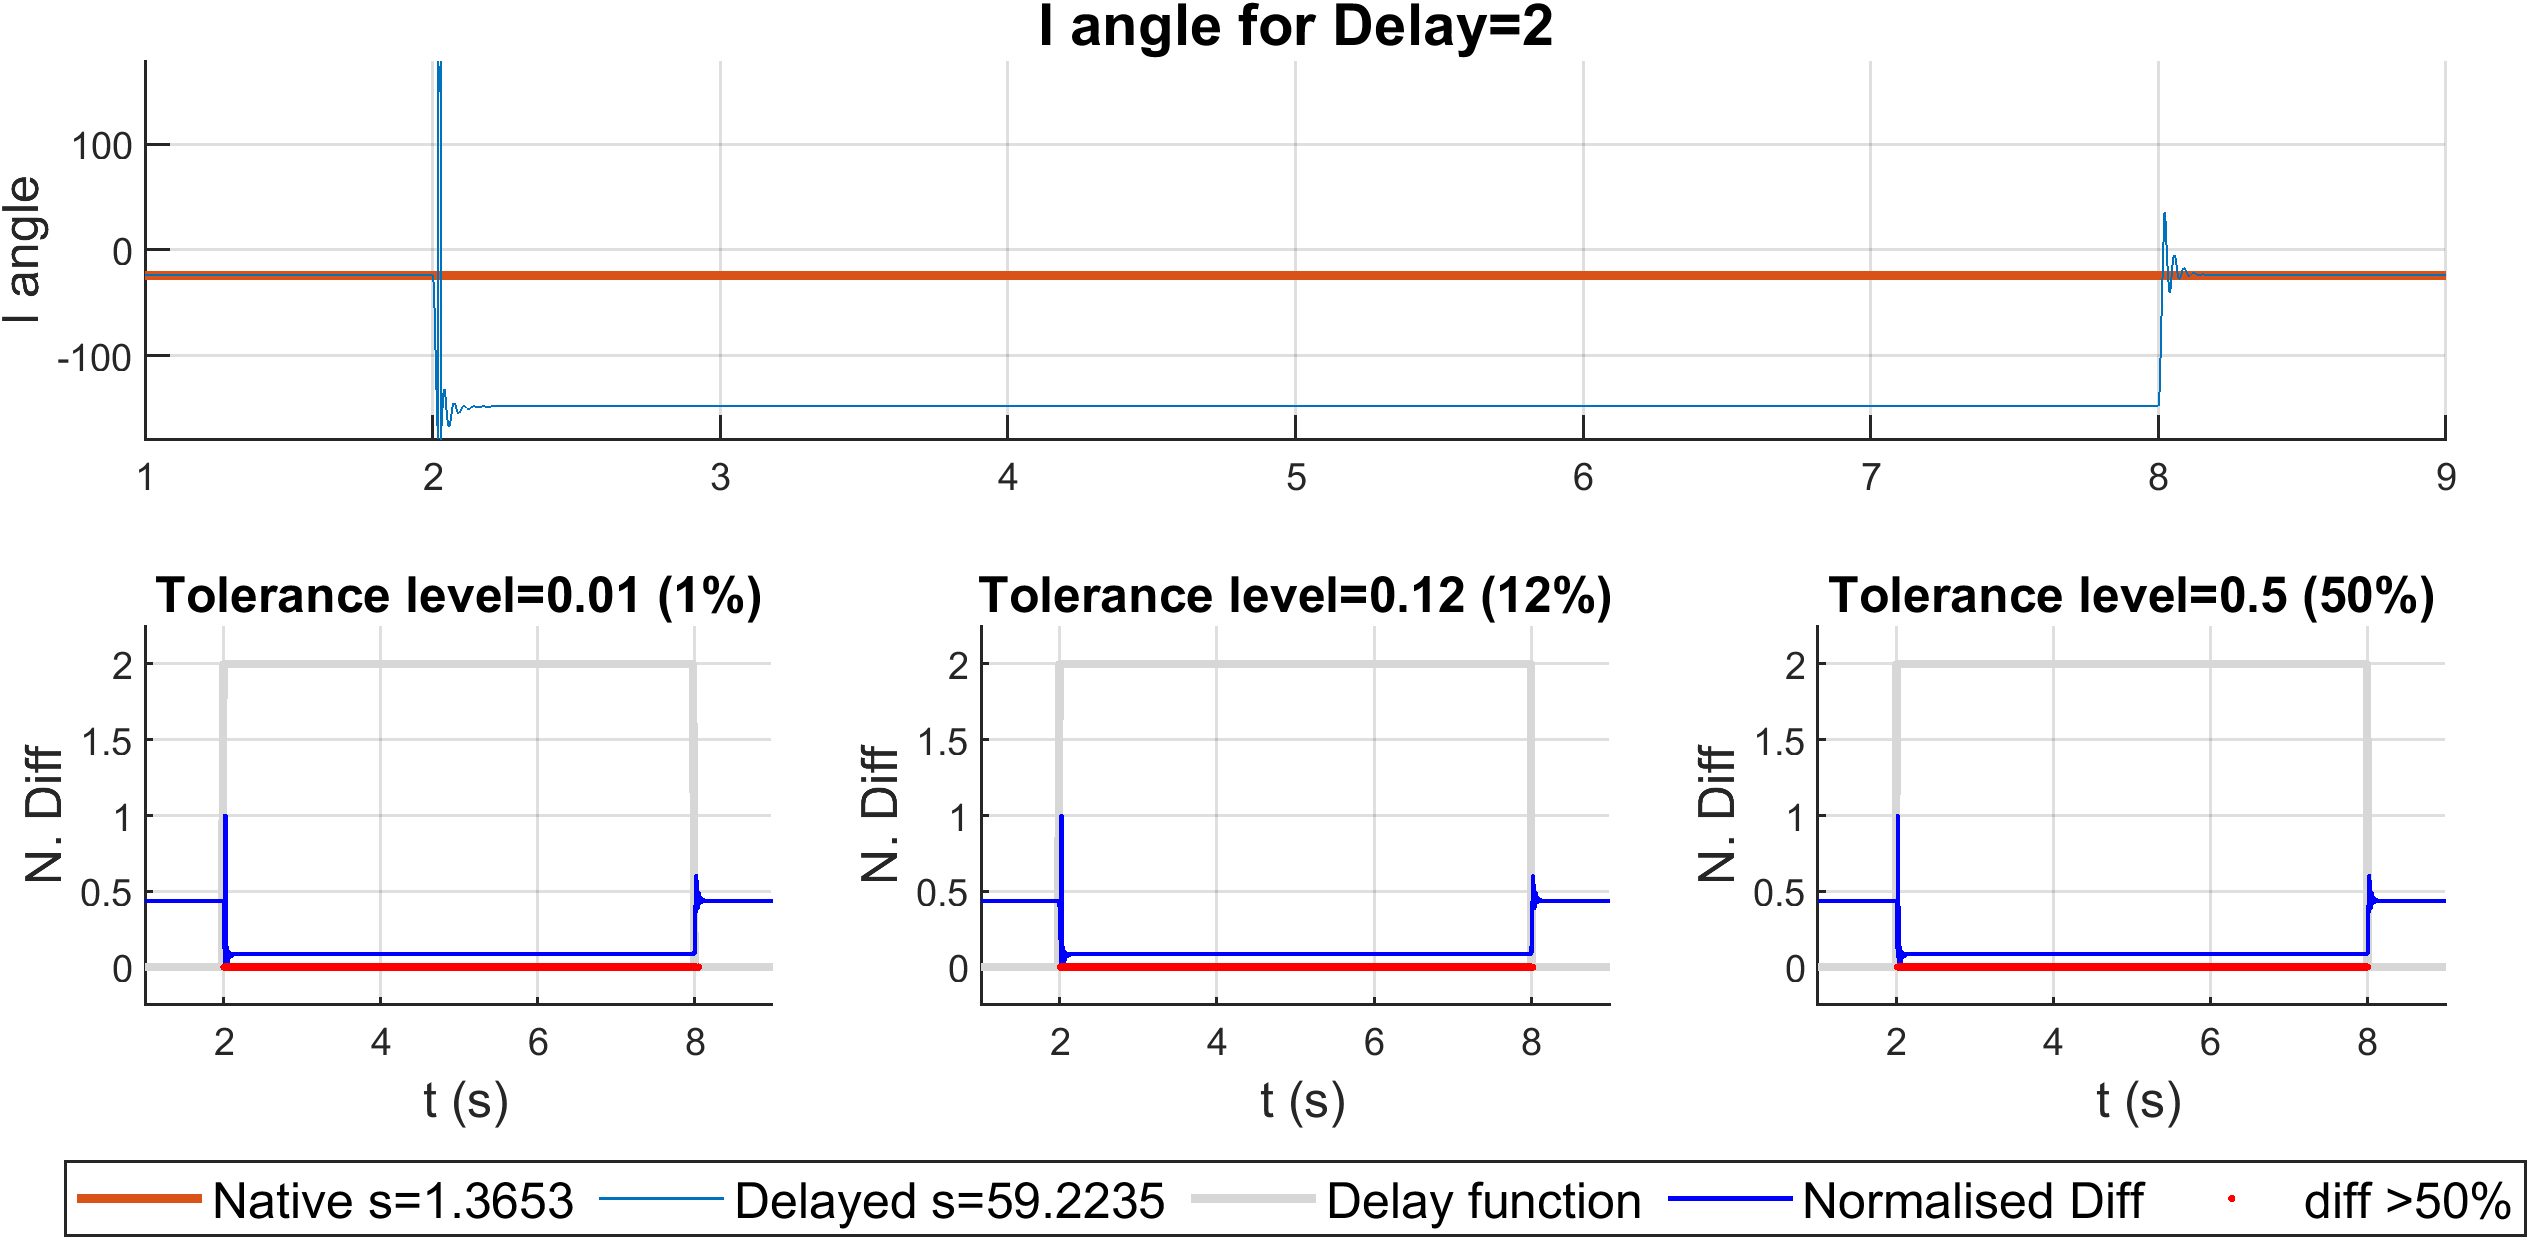
\includegraphics[width=0.95\textwidth]{PMUsim-figures/DelayOf_2/Instant_iAngle.png}}\
 \label{fig:PMUsim_Two_Angle}
 %\caption{Instant Delay Angle Output for the Delay Level of Two}
  \end{tabular}
 \end{table}


\newpage \subsection{Delay Level of Three}


\begin{table}[]
\caption{Results for Magnitude Output}
   \fbox{    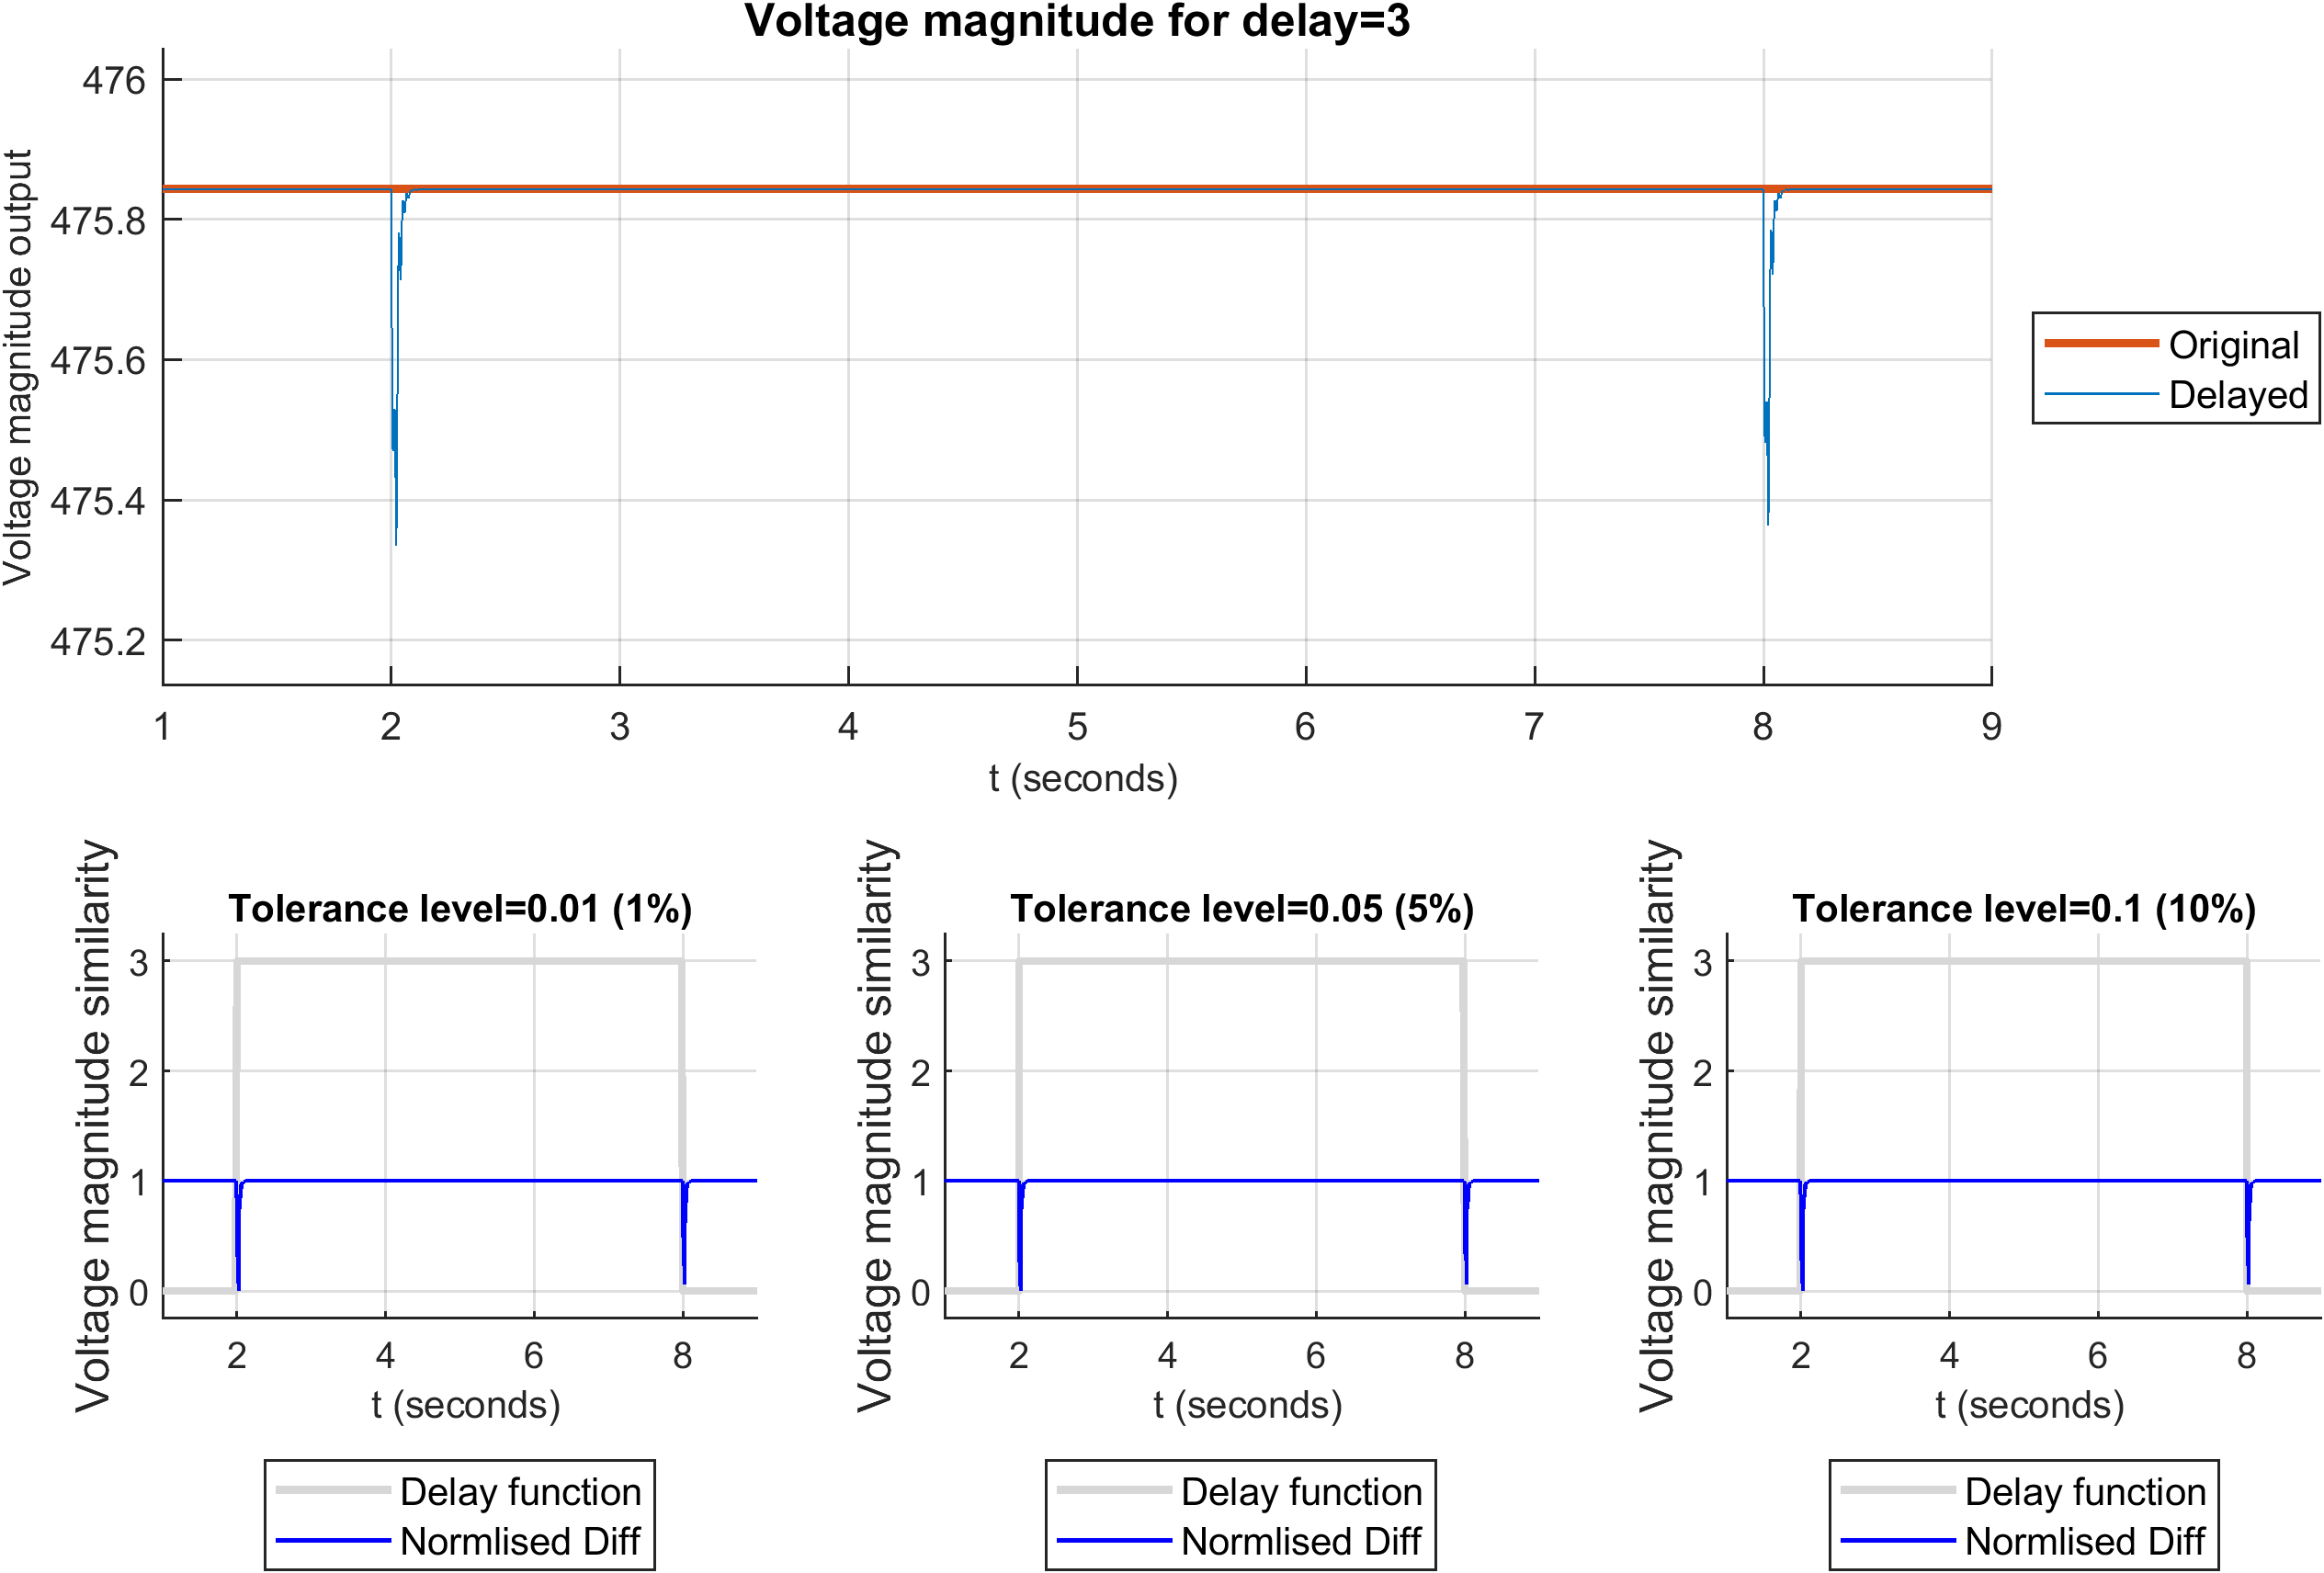
\includegraphics[width=0.95\textwidth]{PMUsim-figures/DelayOf_3/Instant_vMagnitude.png}}\
  
    
   \fbox{  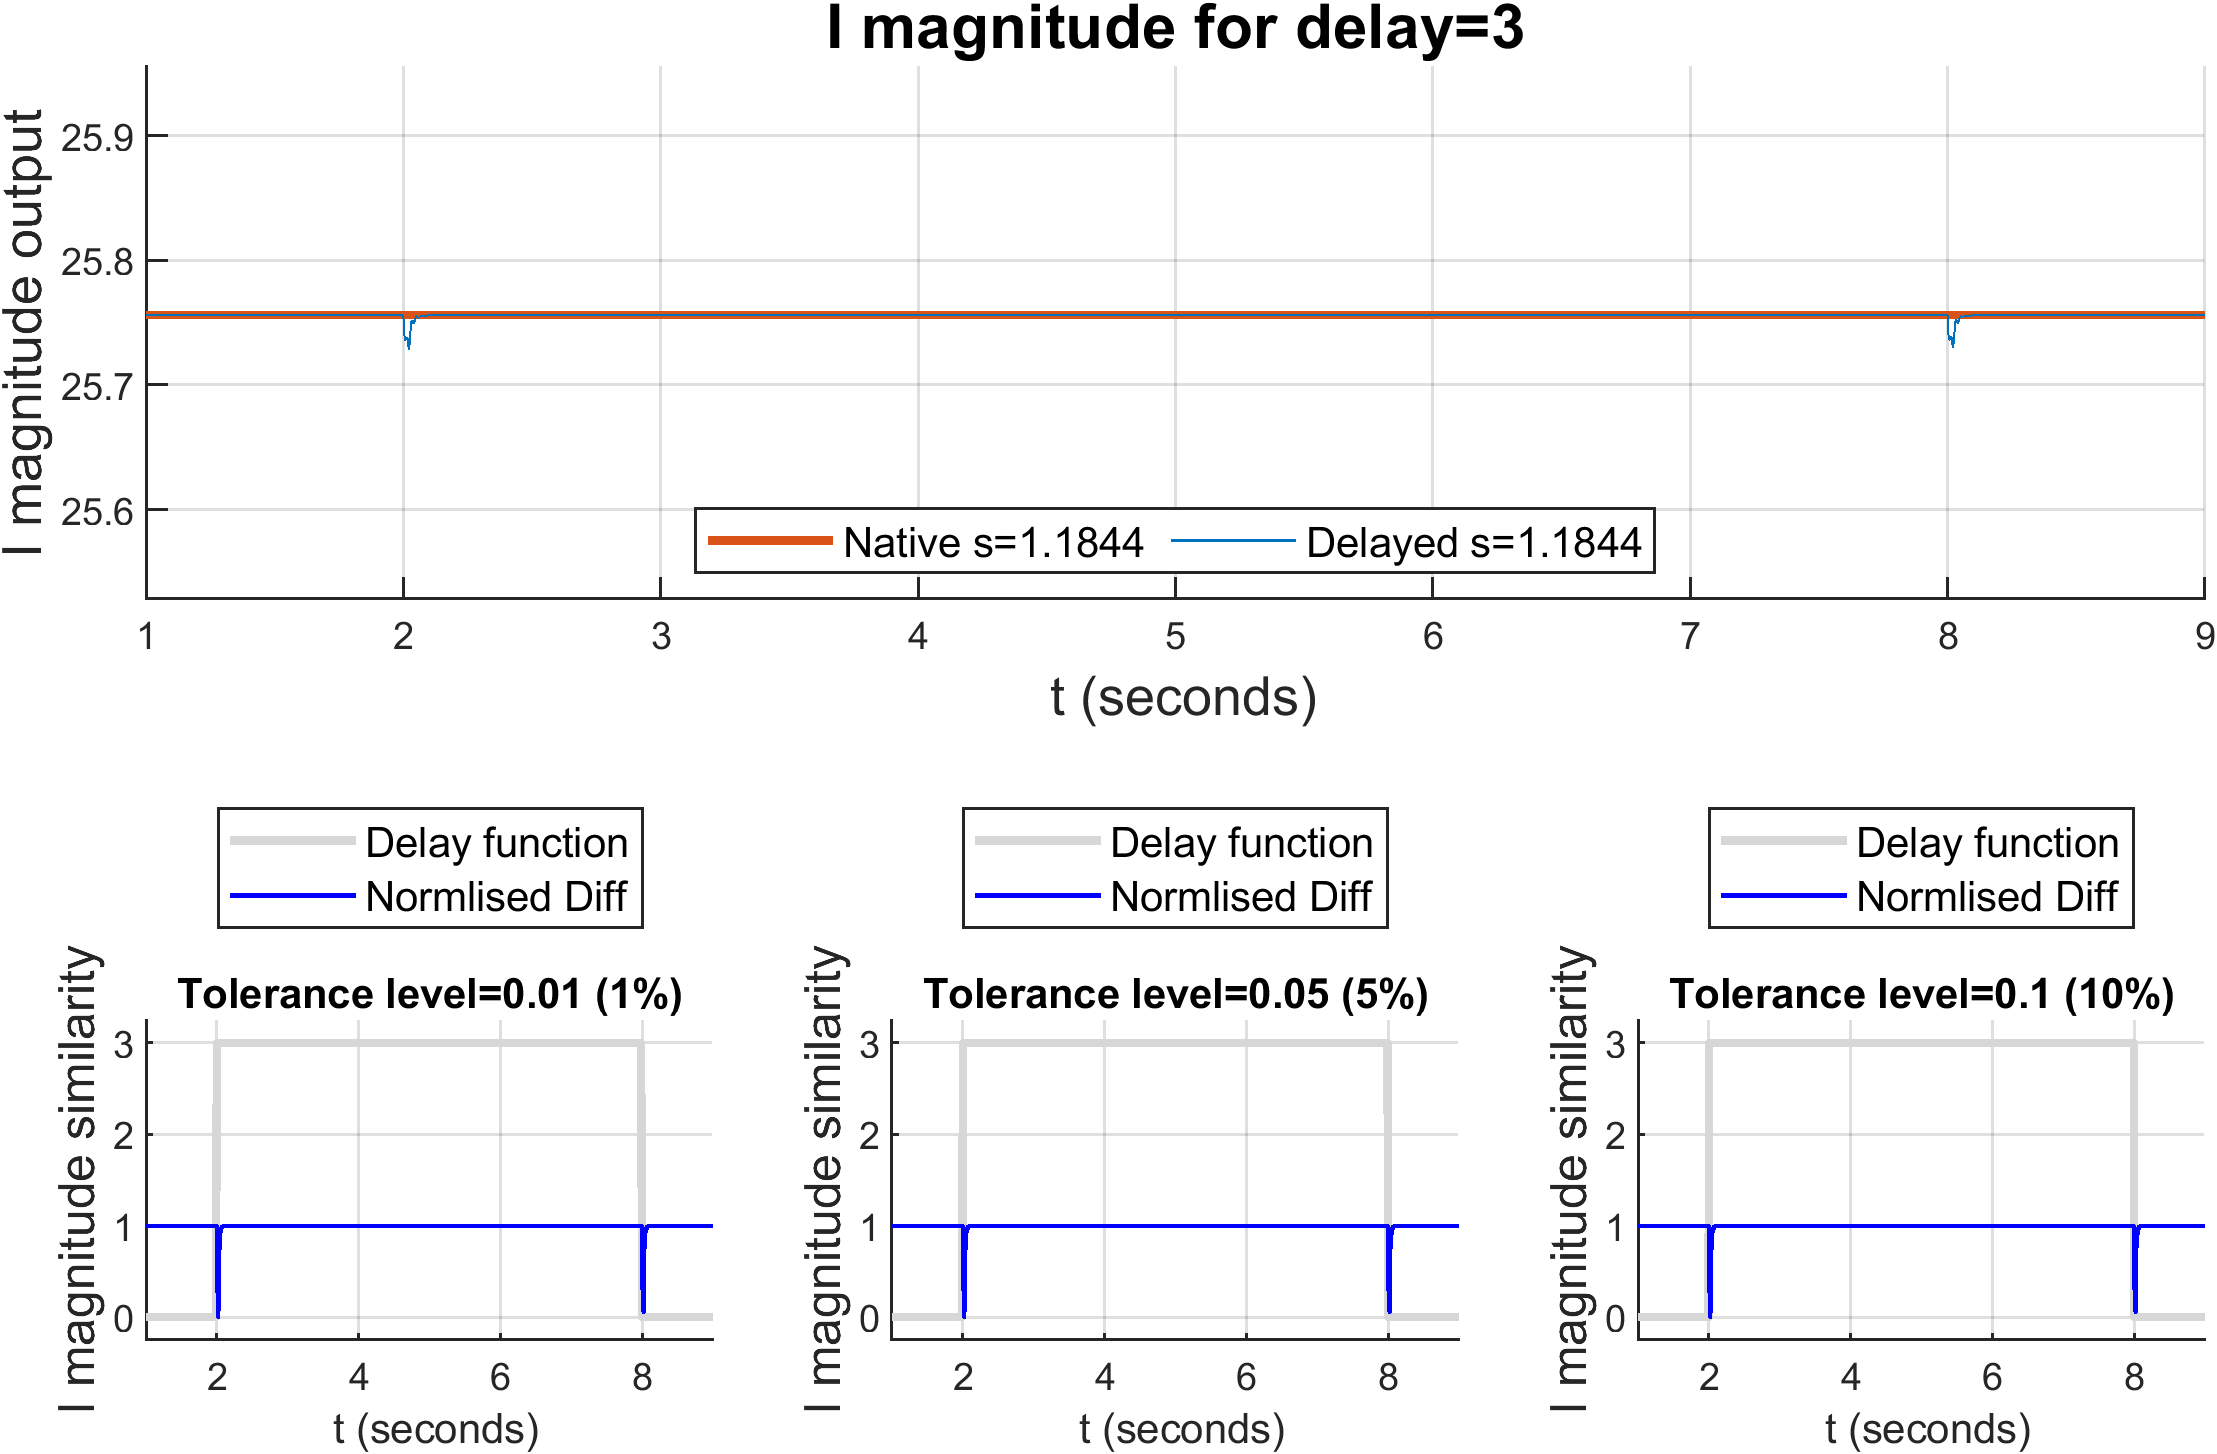
\includegraphics[width=0.95\textwidth]{PMUsim-figures/DelayOf_3/Instant_iMagnitude.png}}\
 \label{fig:PMUsim_Three_Magnitude}
 %\caption{Instant Delay Magnitude Output for the Delay Level of Three}
  \end{tabular}
 \end{table}

\newpage  

\begin{table}[]
\caption{Results for Frequency Output}
   \fbox{    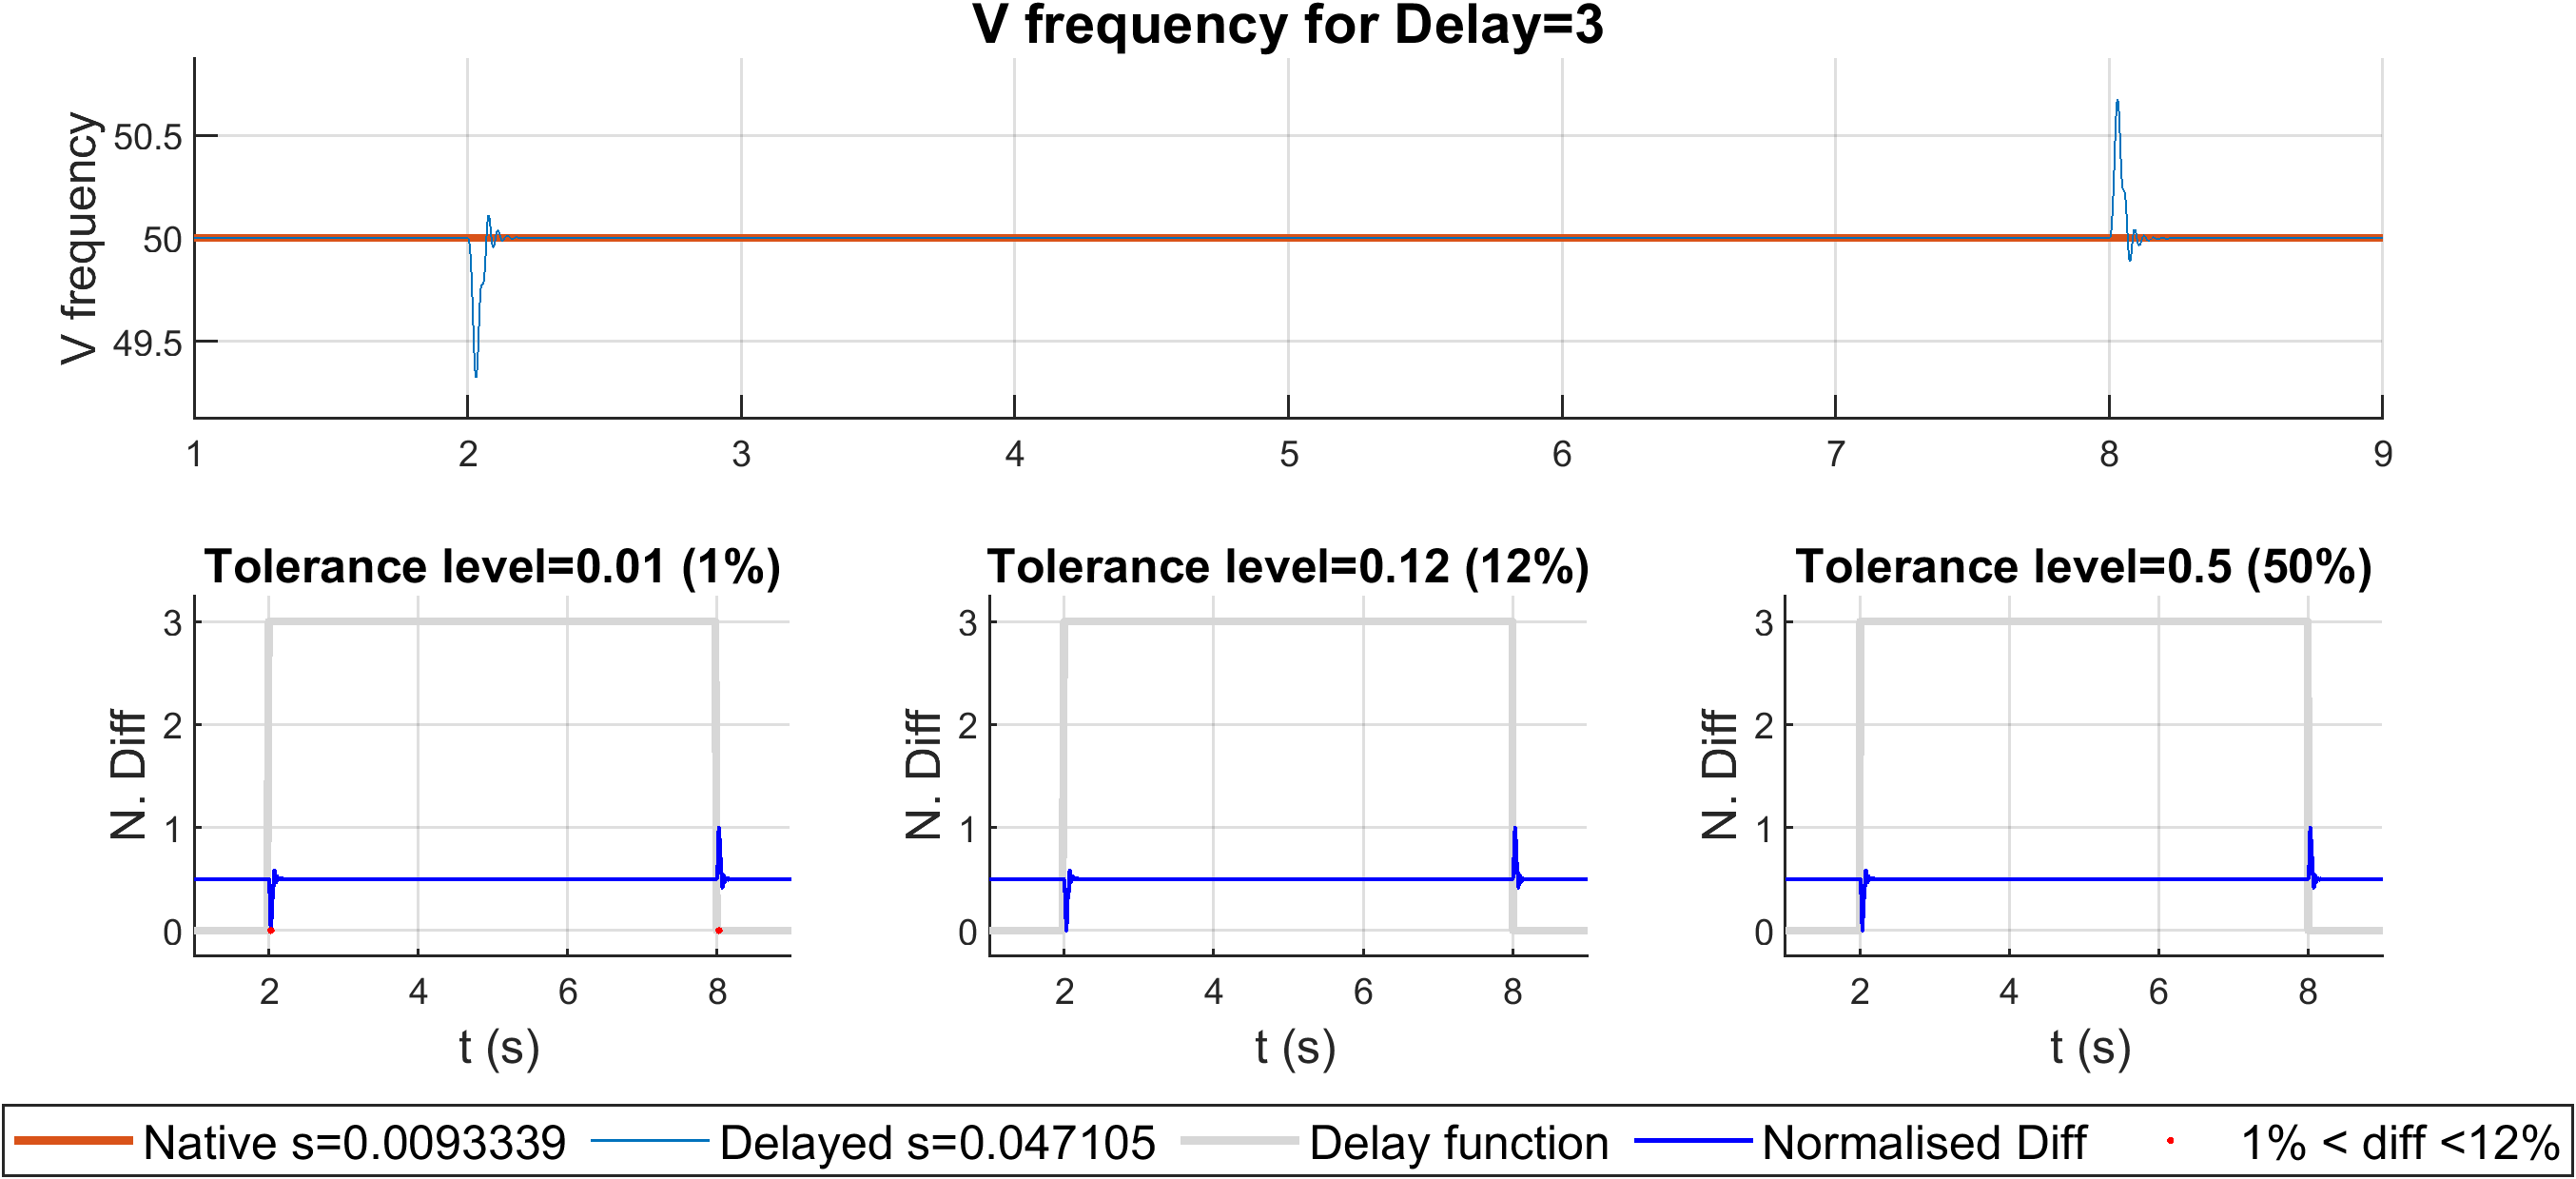
\includegraphics[width=0.95\textwidth]{PMUsim-figures/DelayOf_3/Instant_vFrequency.png}}\
  
    
   \fbox{  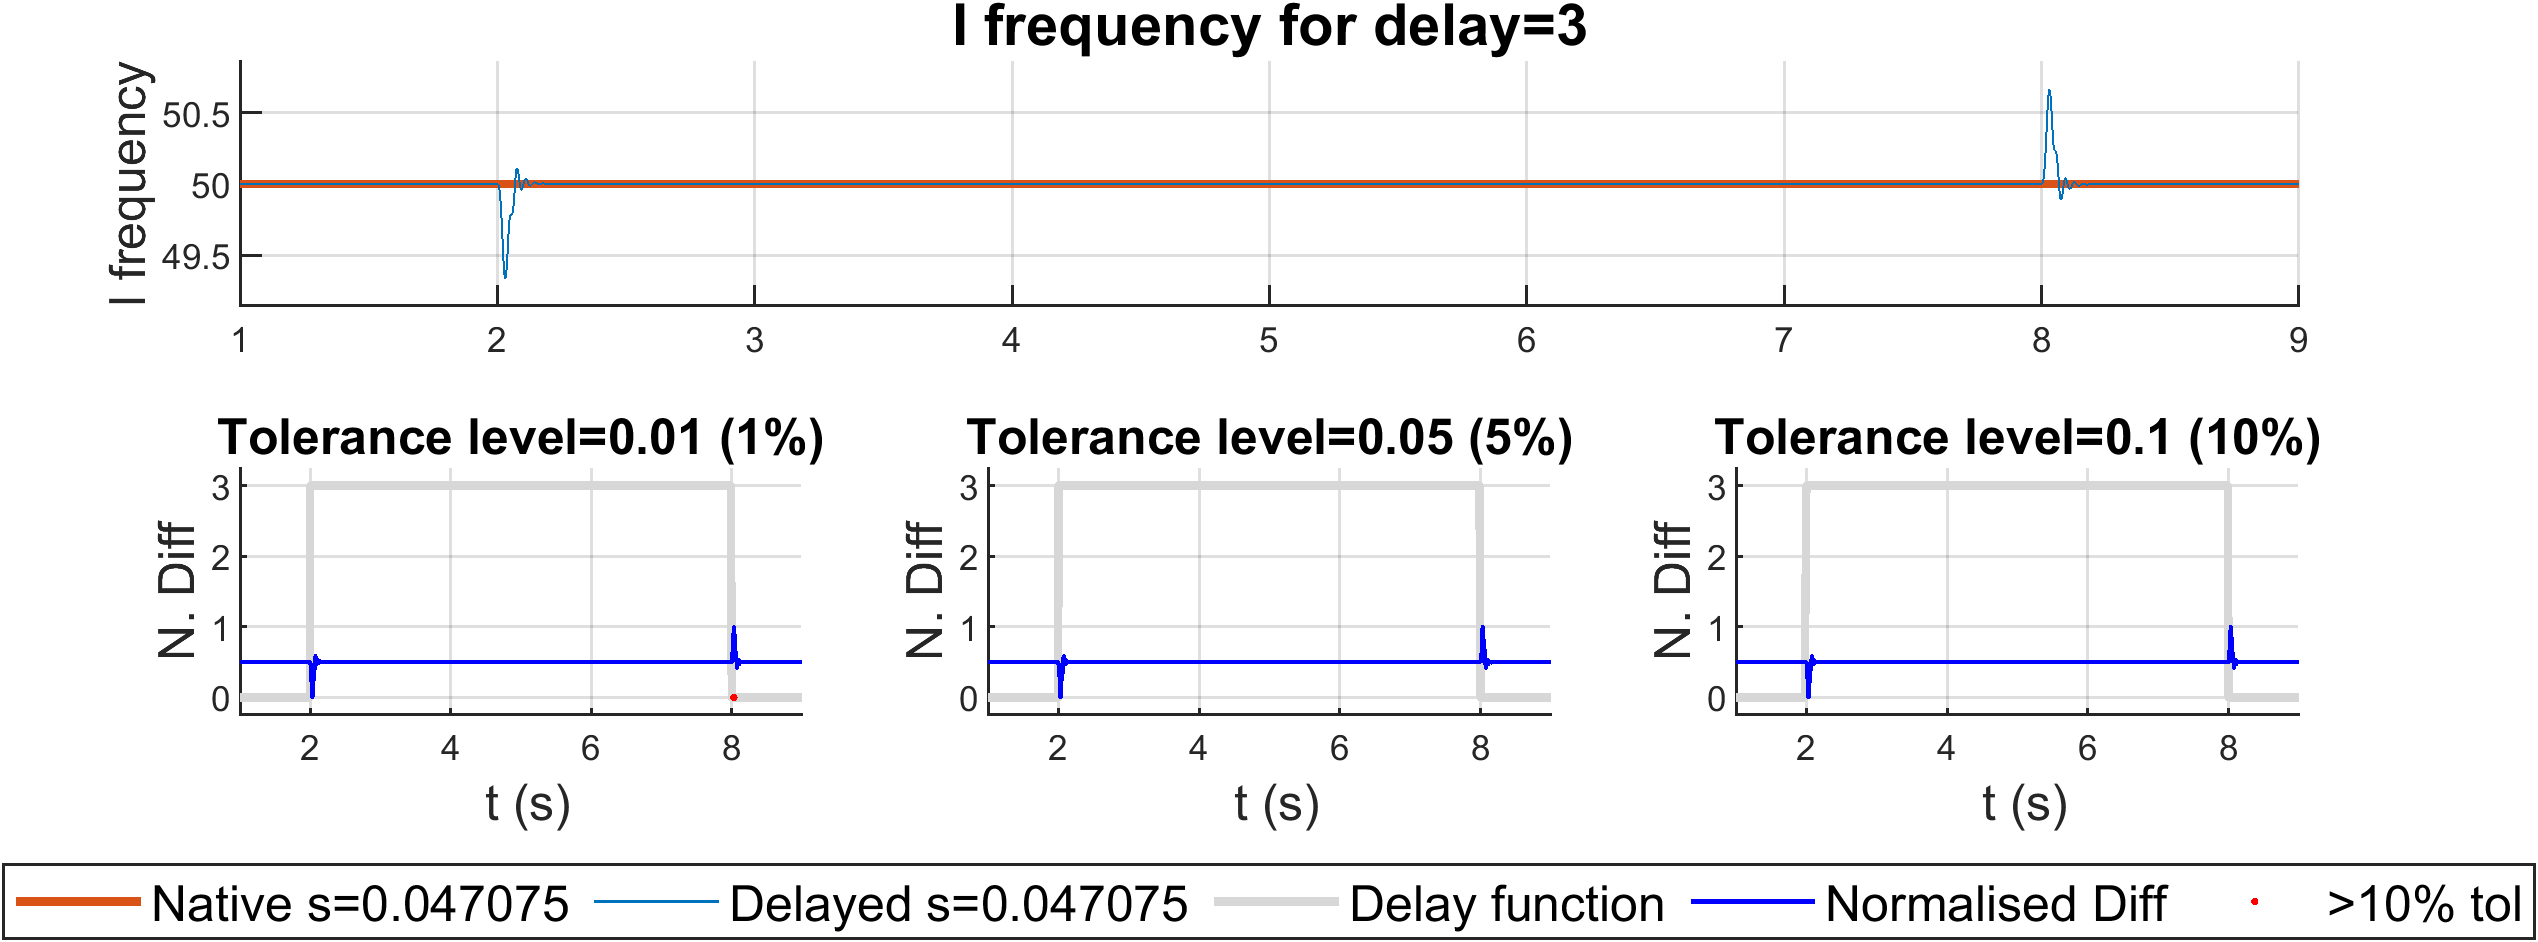
\includegraphics[width=0.95\textwidth]{PMUsim-figures/DelayOf_3/Instant_iFrequency.png}}\
 \label{fig:PMUsim_Three_Frequency}
 %\caption{Instant Delay Frequency Output for the Delay Level of Three}
  \end{tabular}
 \end{table}


\newpage

\begin{table}[]
\caption{Results for Angle Output}
   \fbox{     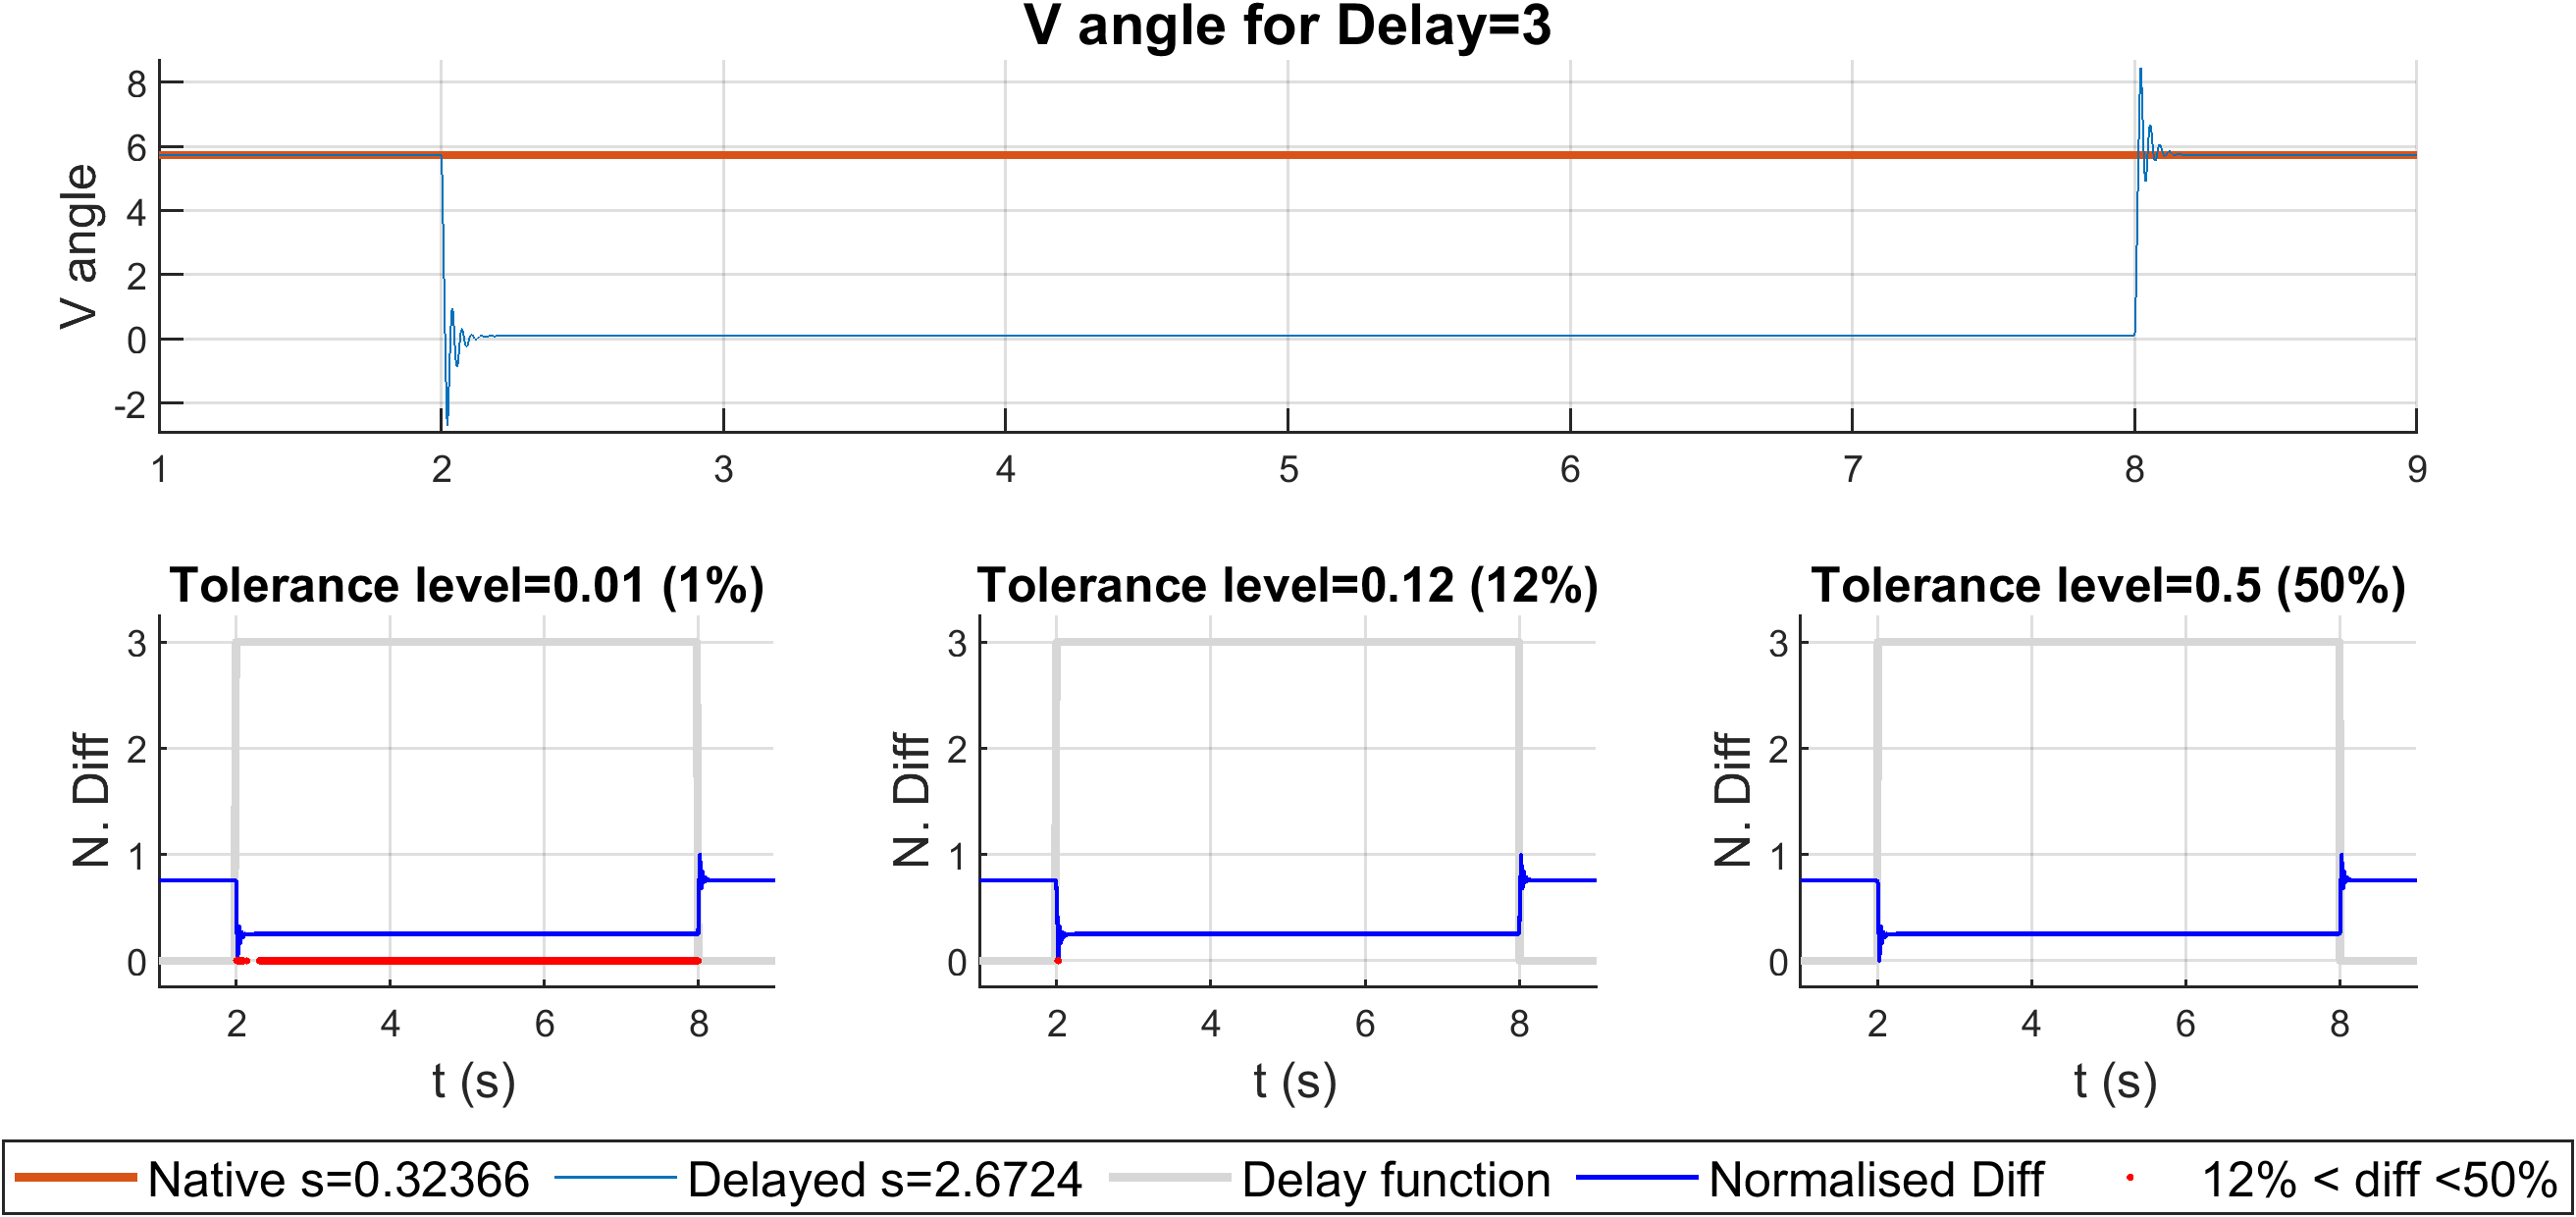
\includegraphics[width=0.95\textwidth]{PMUsim-figures/DelayOf_3/Instant_vAngle.png}}\
  
    
   \fbox{  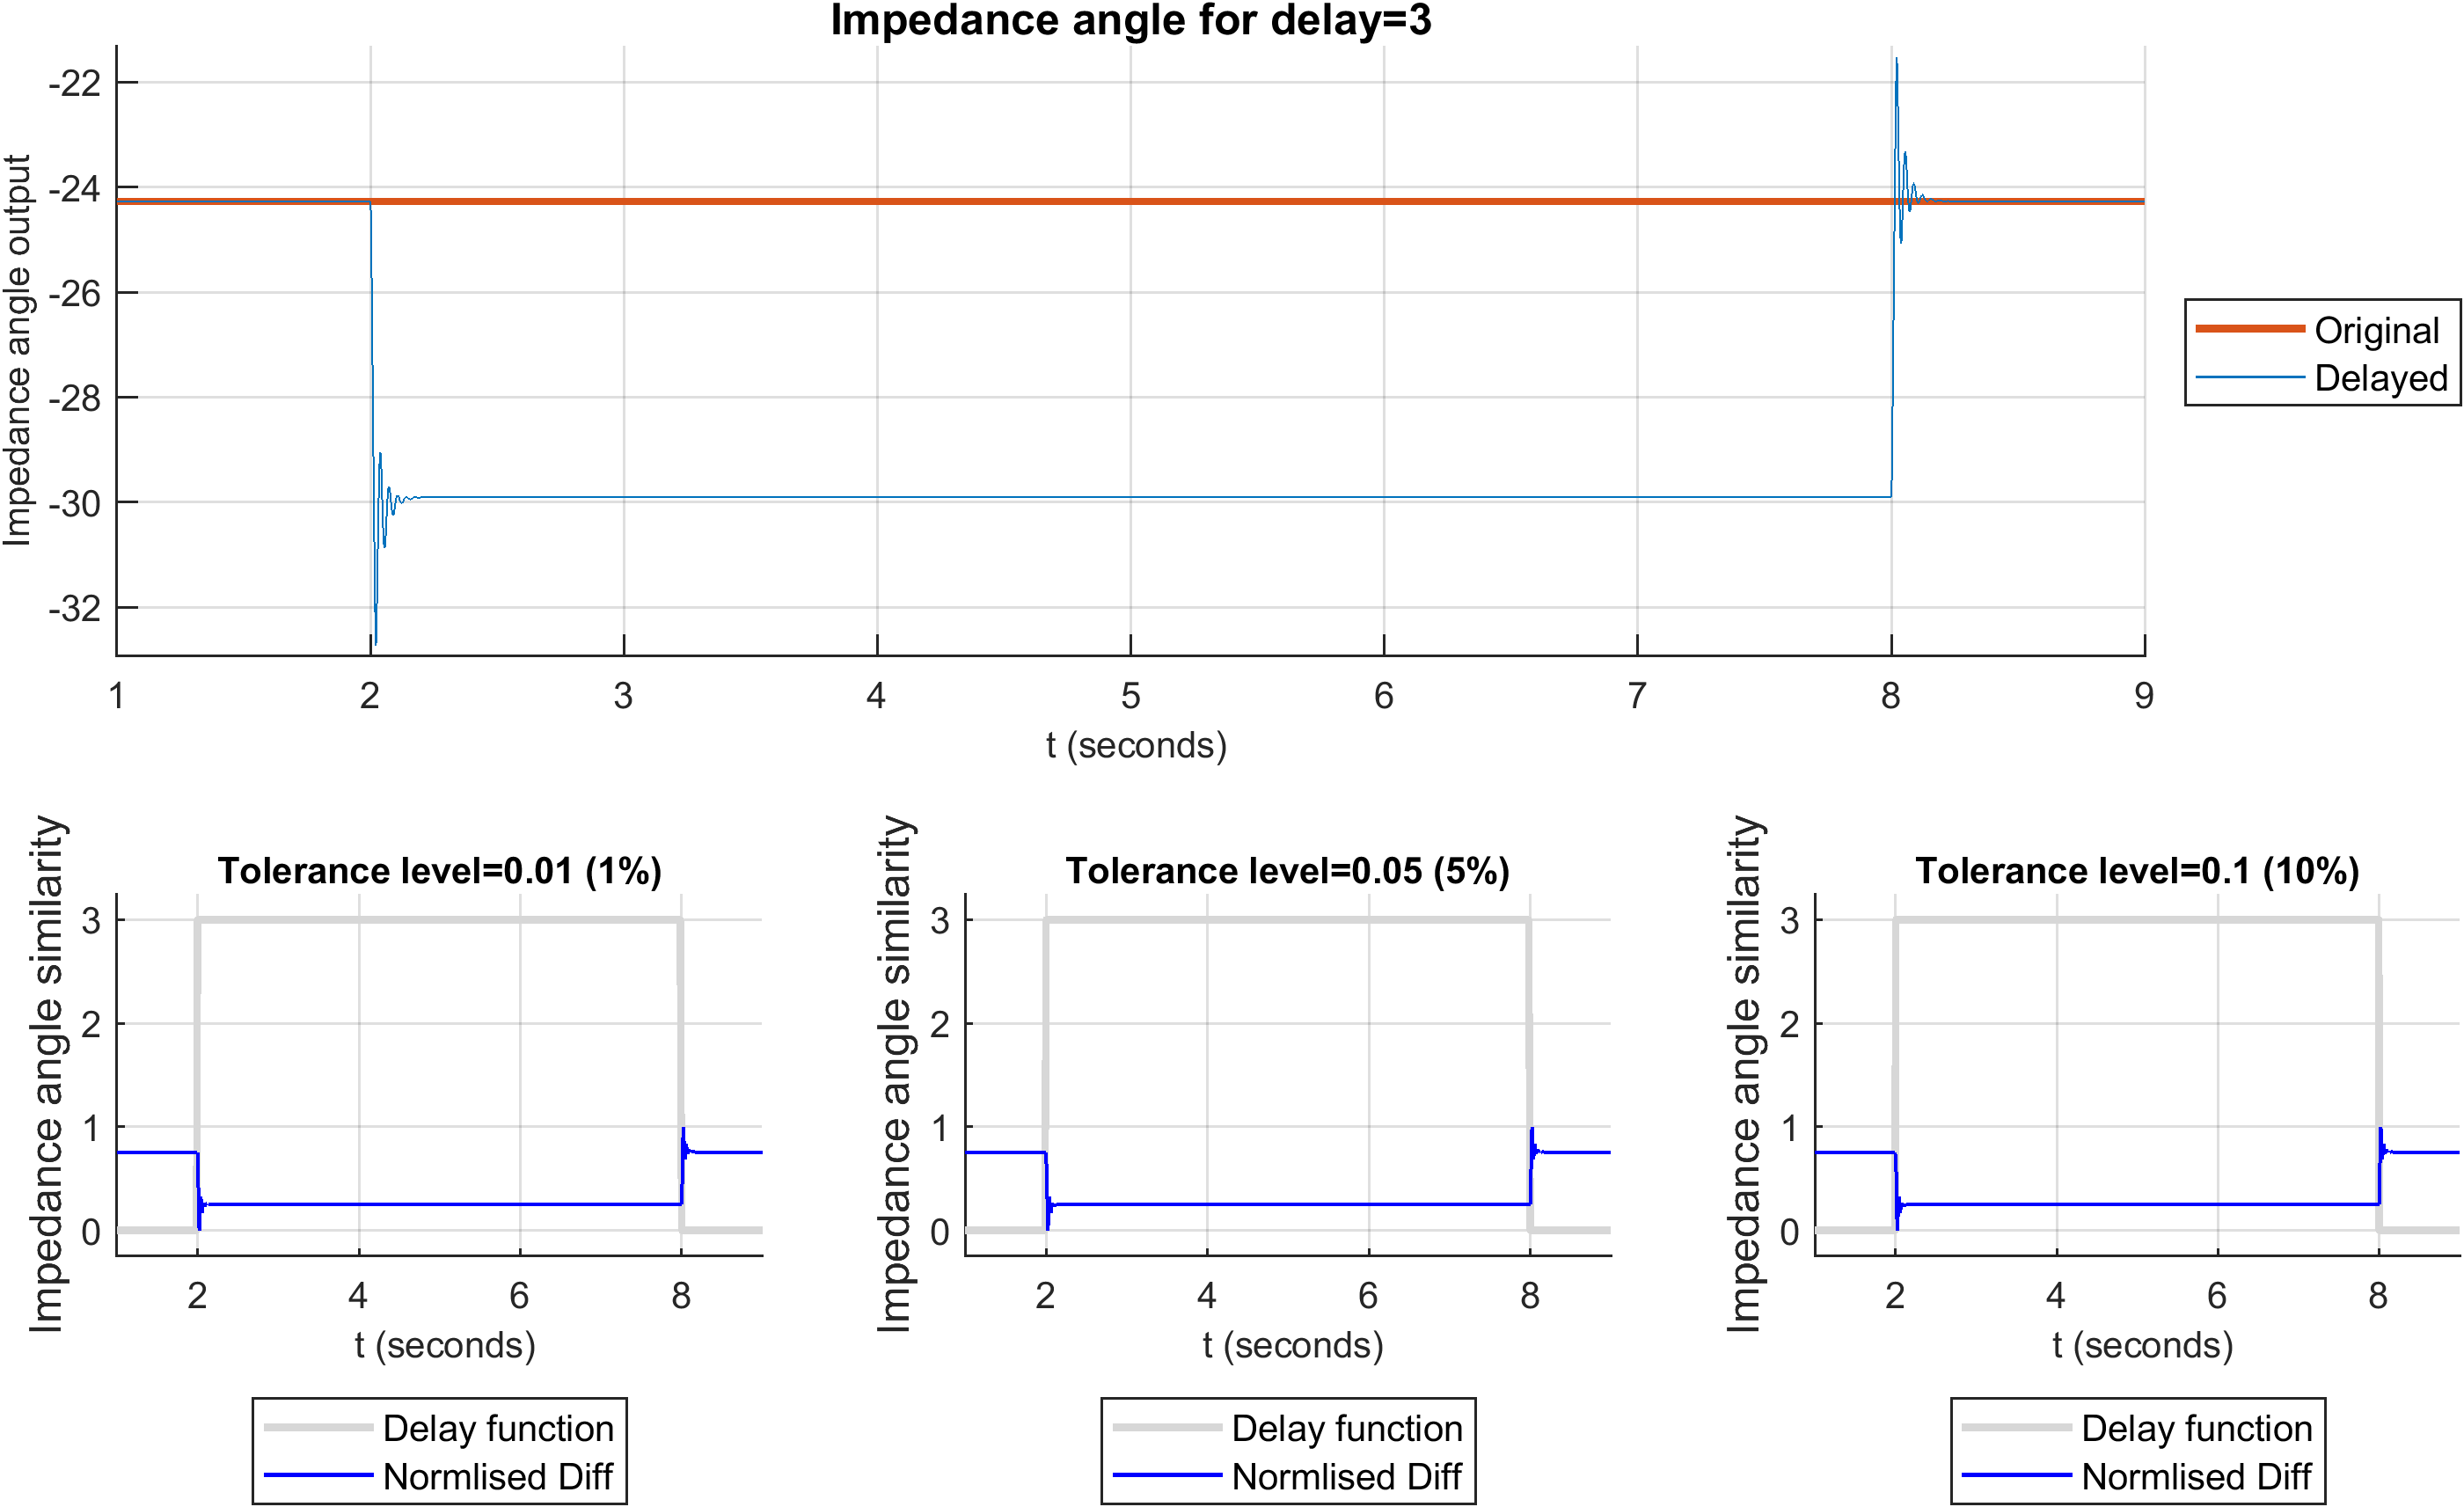
\includegraphics[width=0.95\textwidth]{PMUsim-figures/DelayOf_3/Instant_iAngle.png}}\
 \label{fig:PMUsim_Three_Angle}
 %\caption{Instant Delay Angle Output for the Delay Level of Three}
  \end{tabular}
 \end{table}

\newpage \subsection{Delay Level of Four}


\begin{table}[]
\caption{Results for Magnitude Output}
   \fbox{    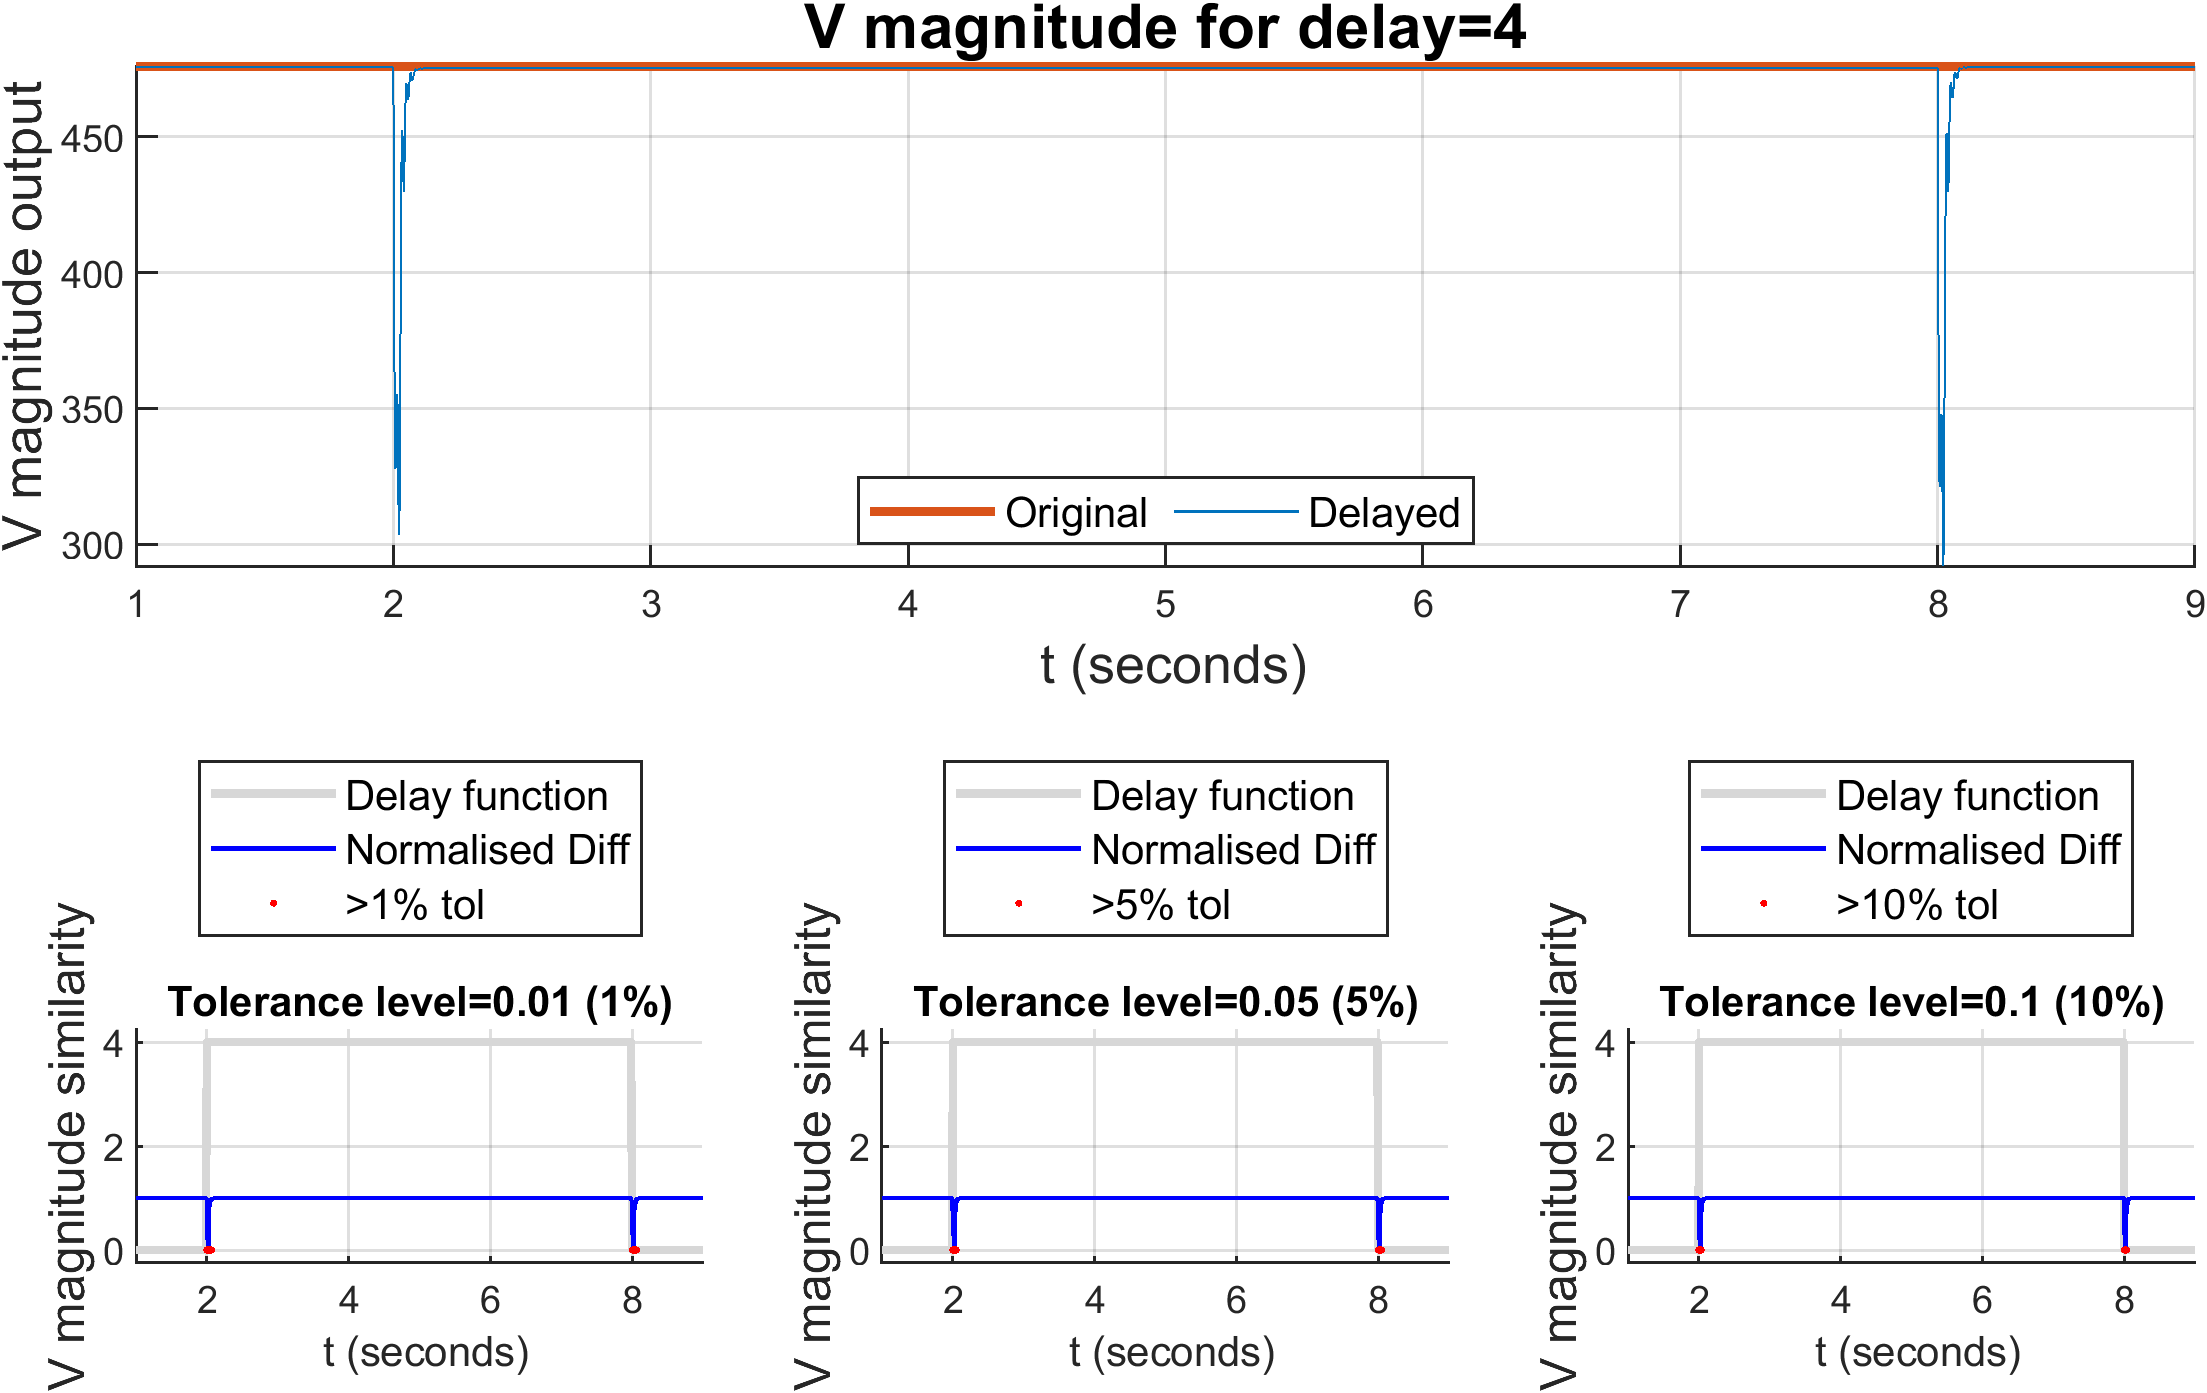
\includegraphics[width=0.95\textwidth]{PMUsim-figures/DelayOf_4/Instant_vMagnitude.png}}\
  
    
   \fbox{   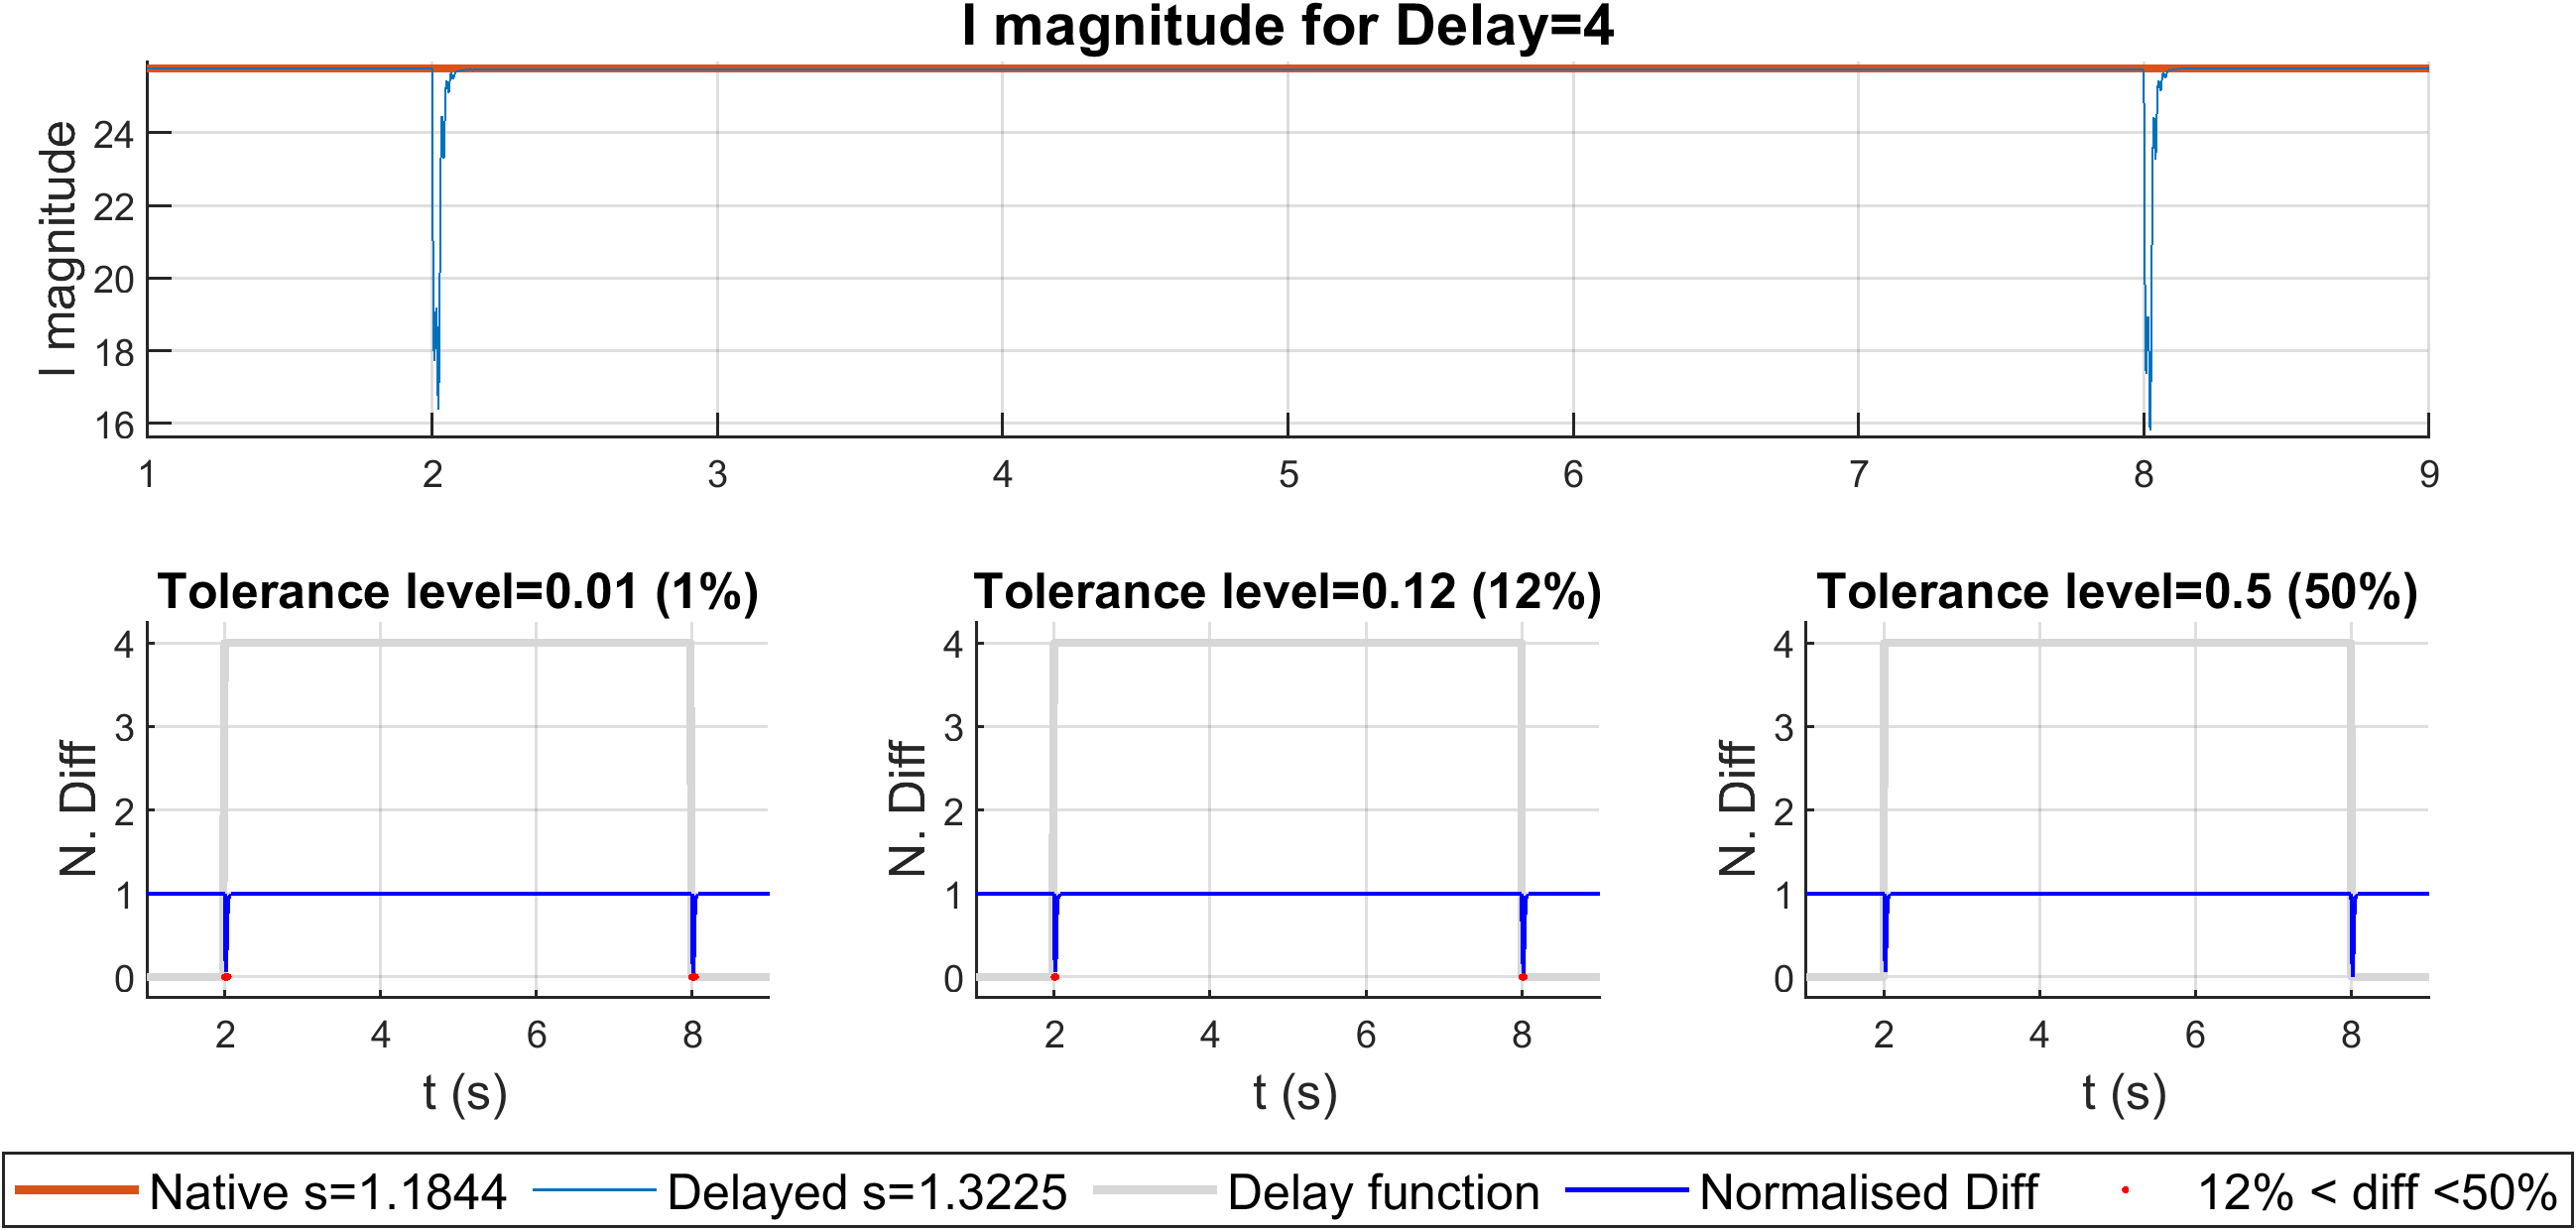
\includegraphics[width=0.95\textwidth]{PMUsim-figures/DelayOf_4/Instant_iMagnitude.png}}\       
\label{fig:PMUsim_Four_Magnitude}
 %\caption{Instant Delay Magnitude Output for the Delay Level of Four}
  \end{tabular}
 \end{table}


\newpage  

\begin{table}[]
\caption{Results for Frequency Output}
   \fbox{     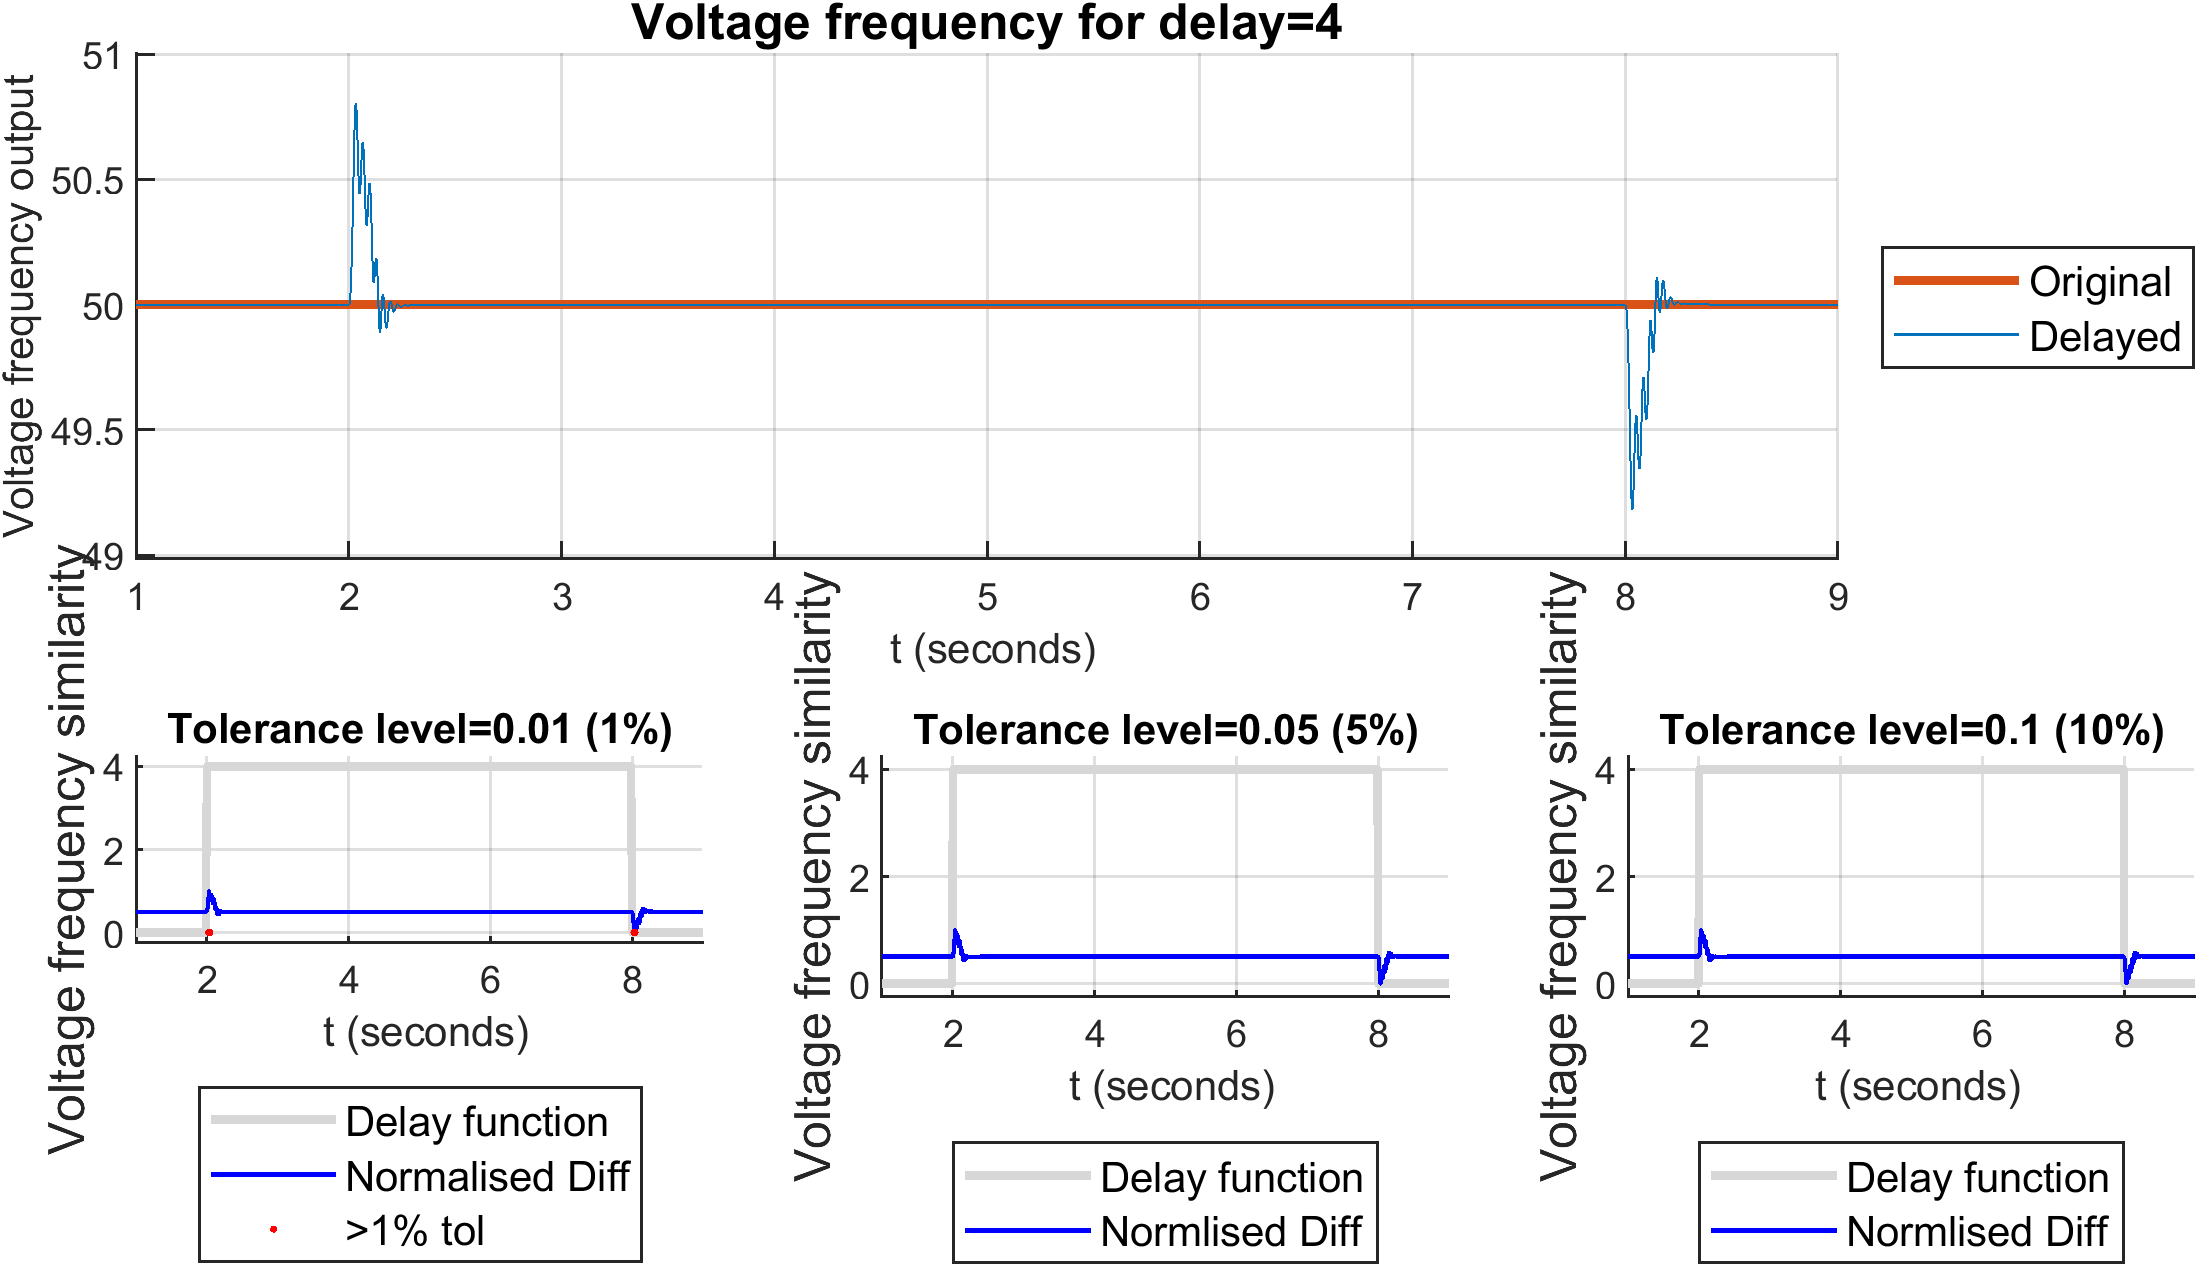
\includegraphics[width=0.95\textwidth]{PMUsim-figures/DelayOf_4/Instant_vFrequency.png}}\
  
    
   \fbox{  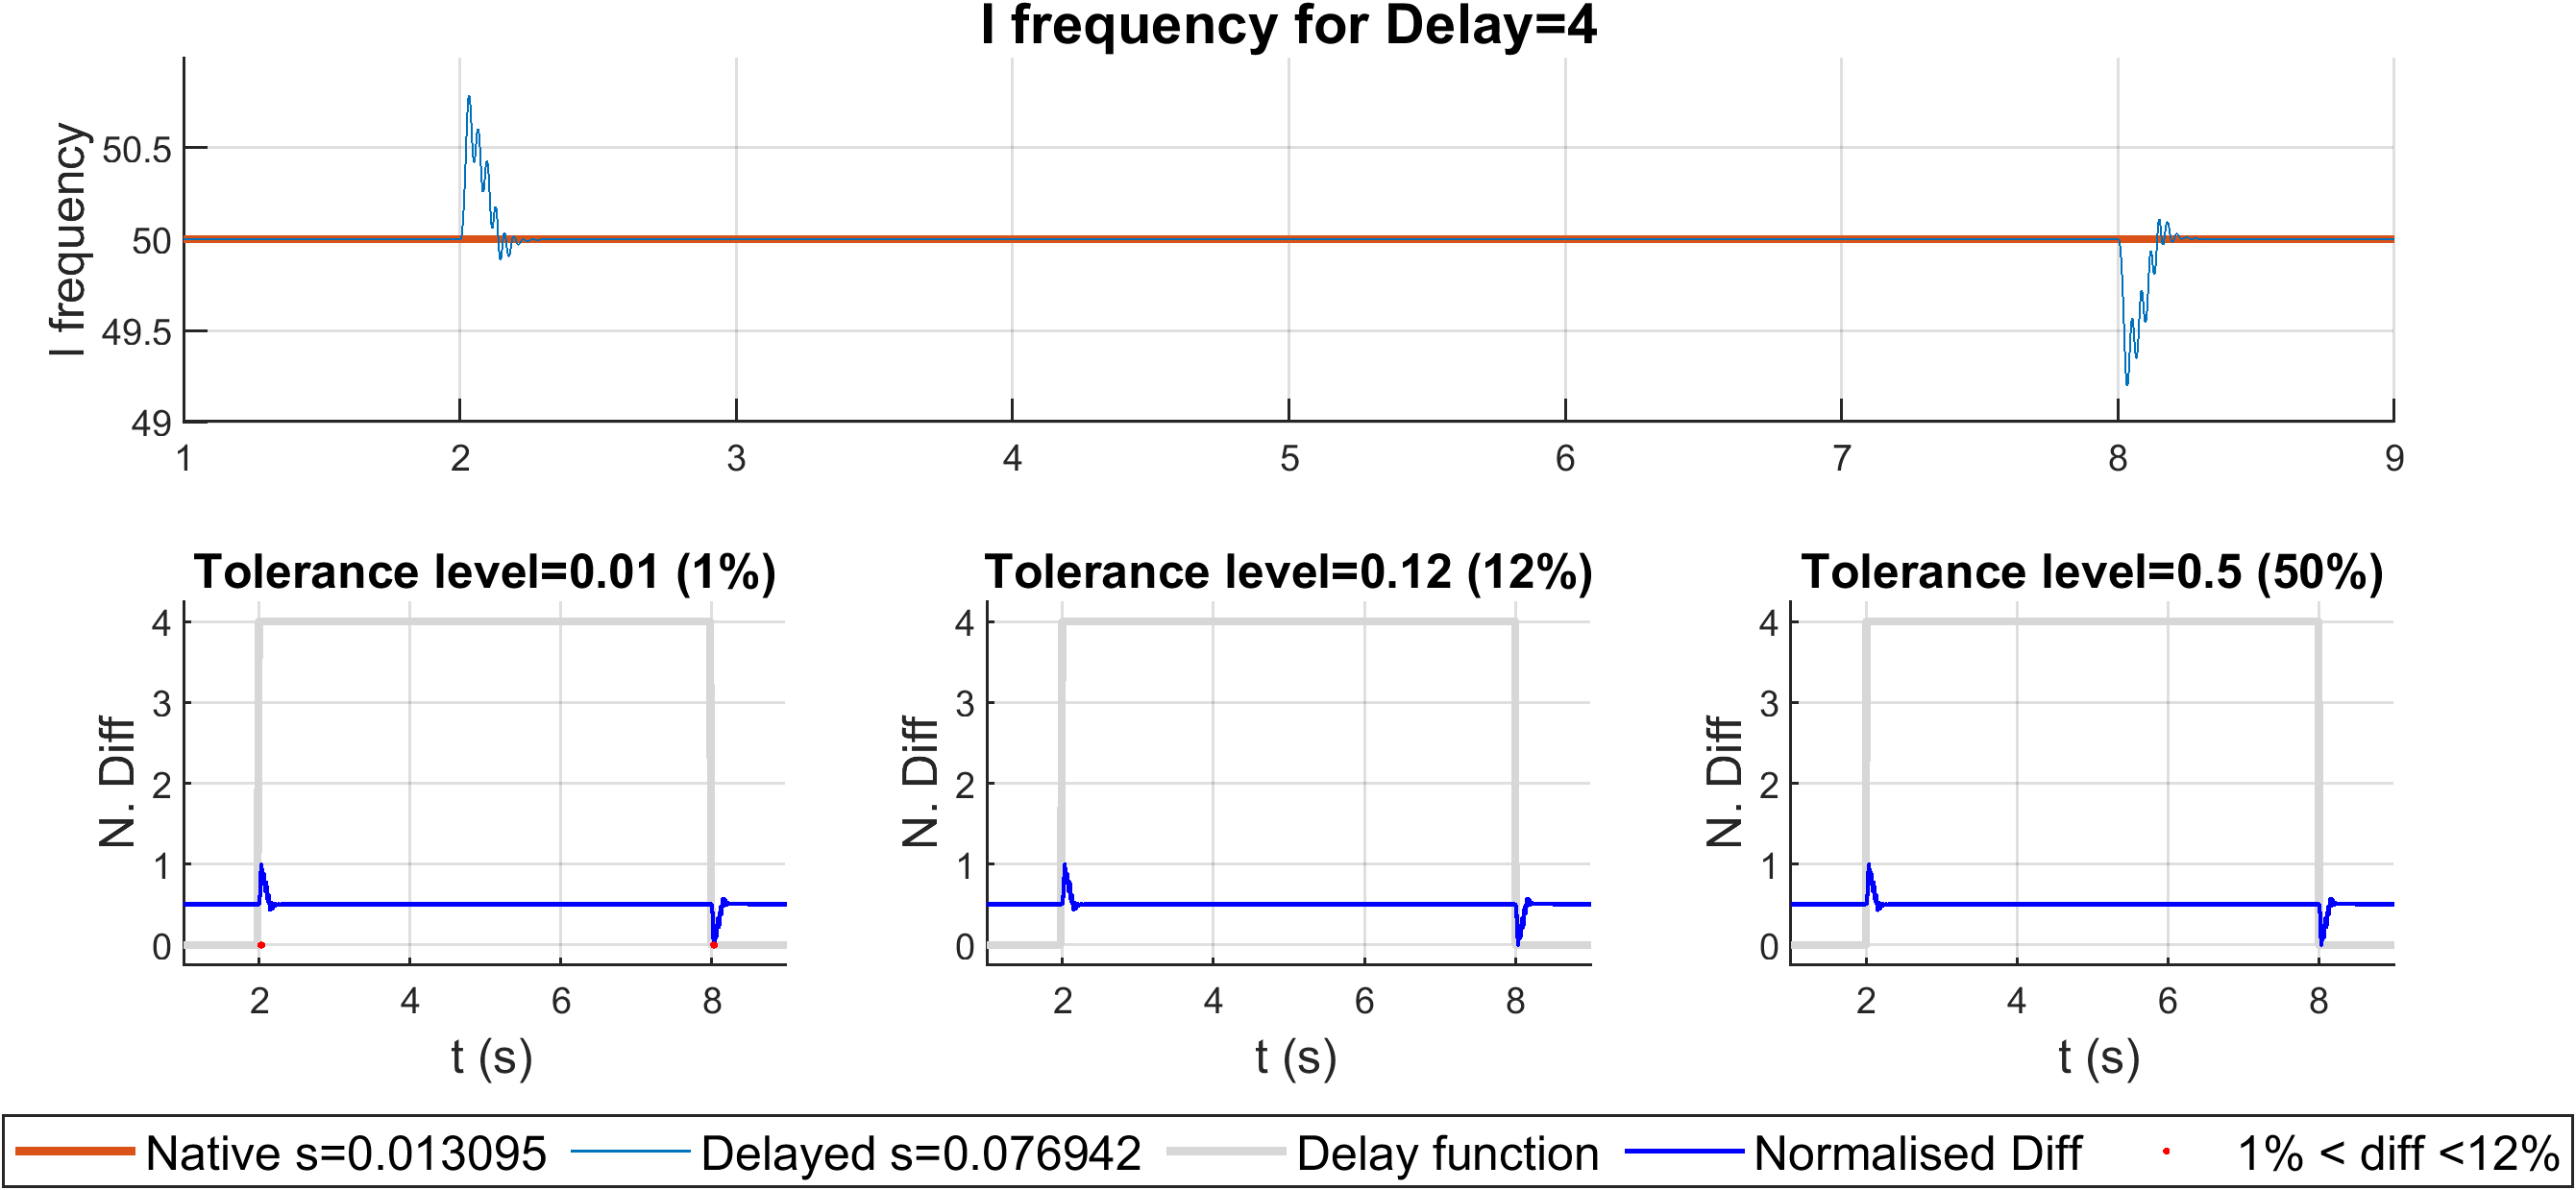
\includegraphics[width=0.95\textwidth]{PMUsim-figures/DelayOf_4/Instant_iFrequency.png}}\ 
 \label{fig:PMUsim_Four_Frequency}
 %\caption{Instant Delay Frequency Output for the Delay Level of Four}
  \end{tabular}
 \end{table}
 

\newpage

\begin{table}[]
\caption{Results for Angle Output}
   \fbox{     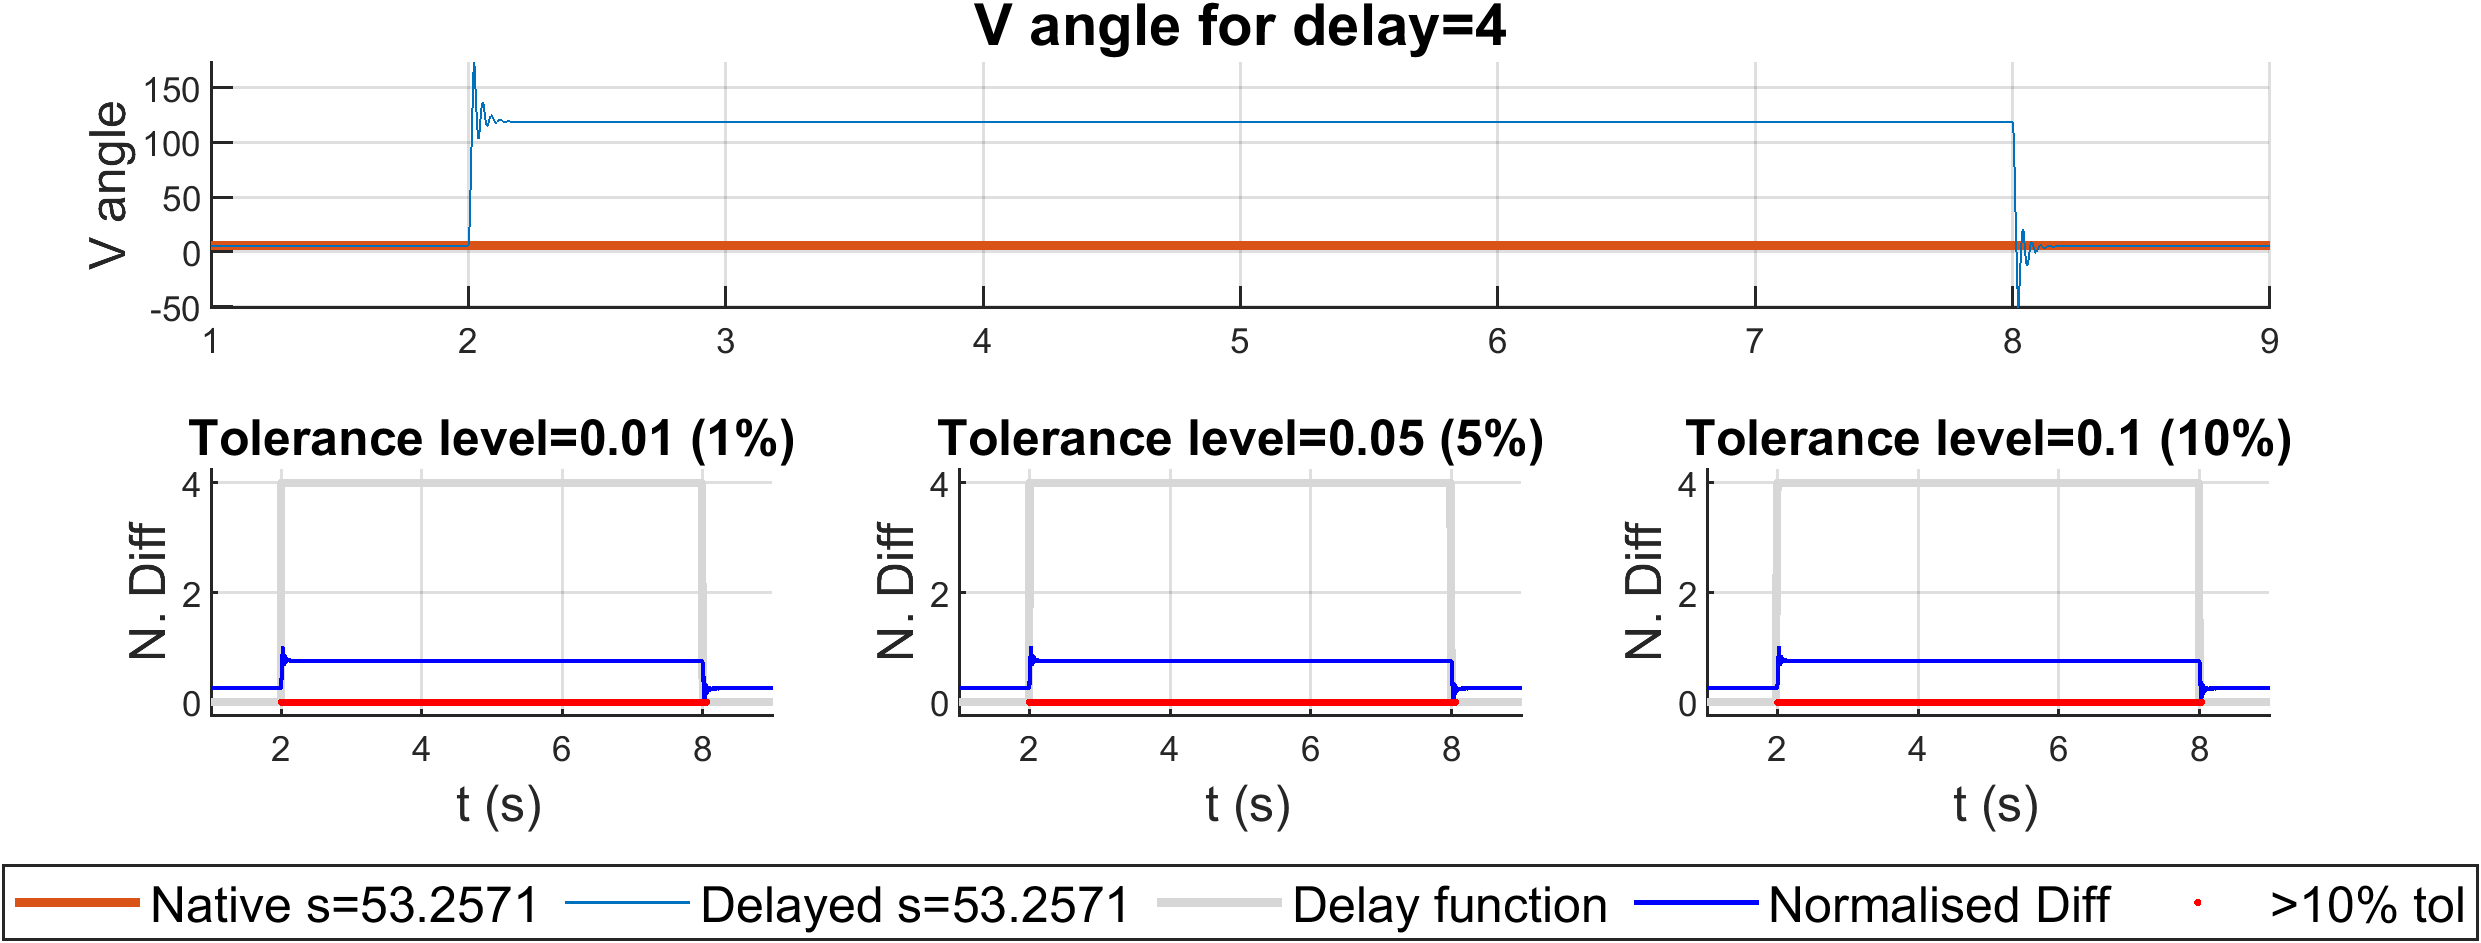
\includegraphics[width=0.95\textwidth]{PMUsim-figures/DelayOf_4/Instant_vAngle.png}}\
  
    
   \fbox{  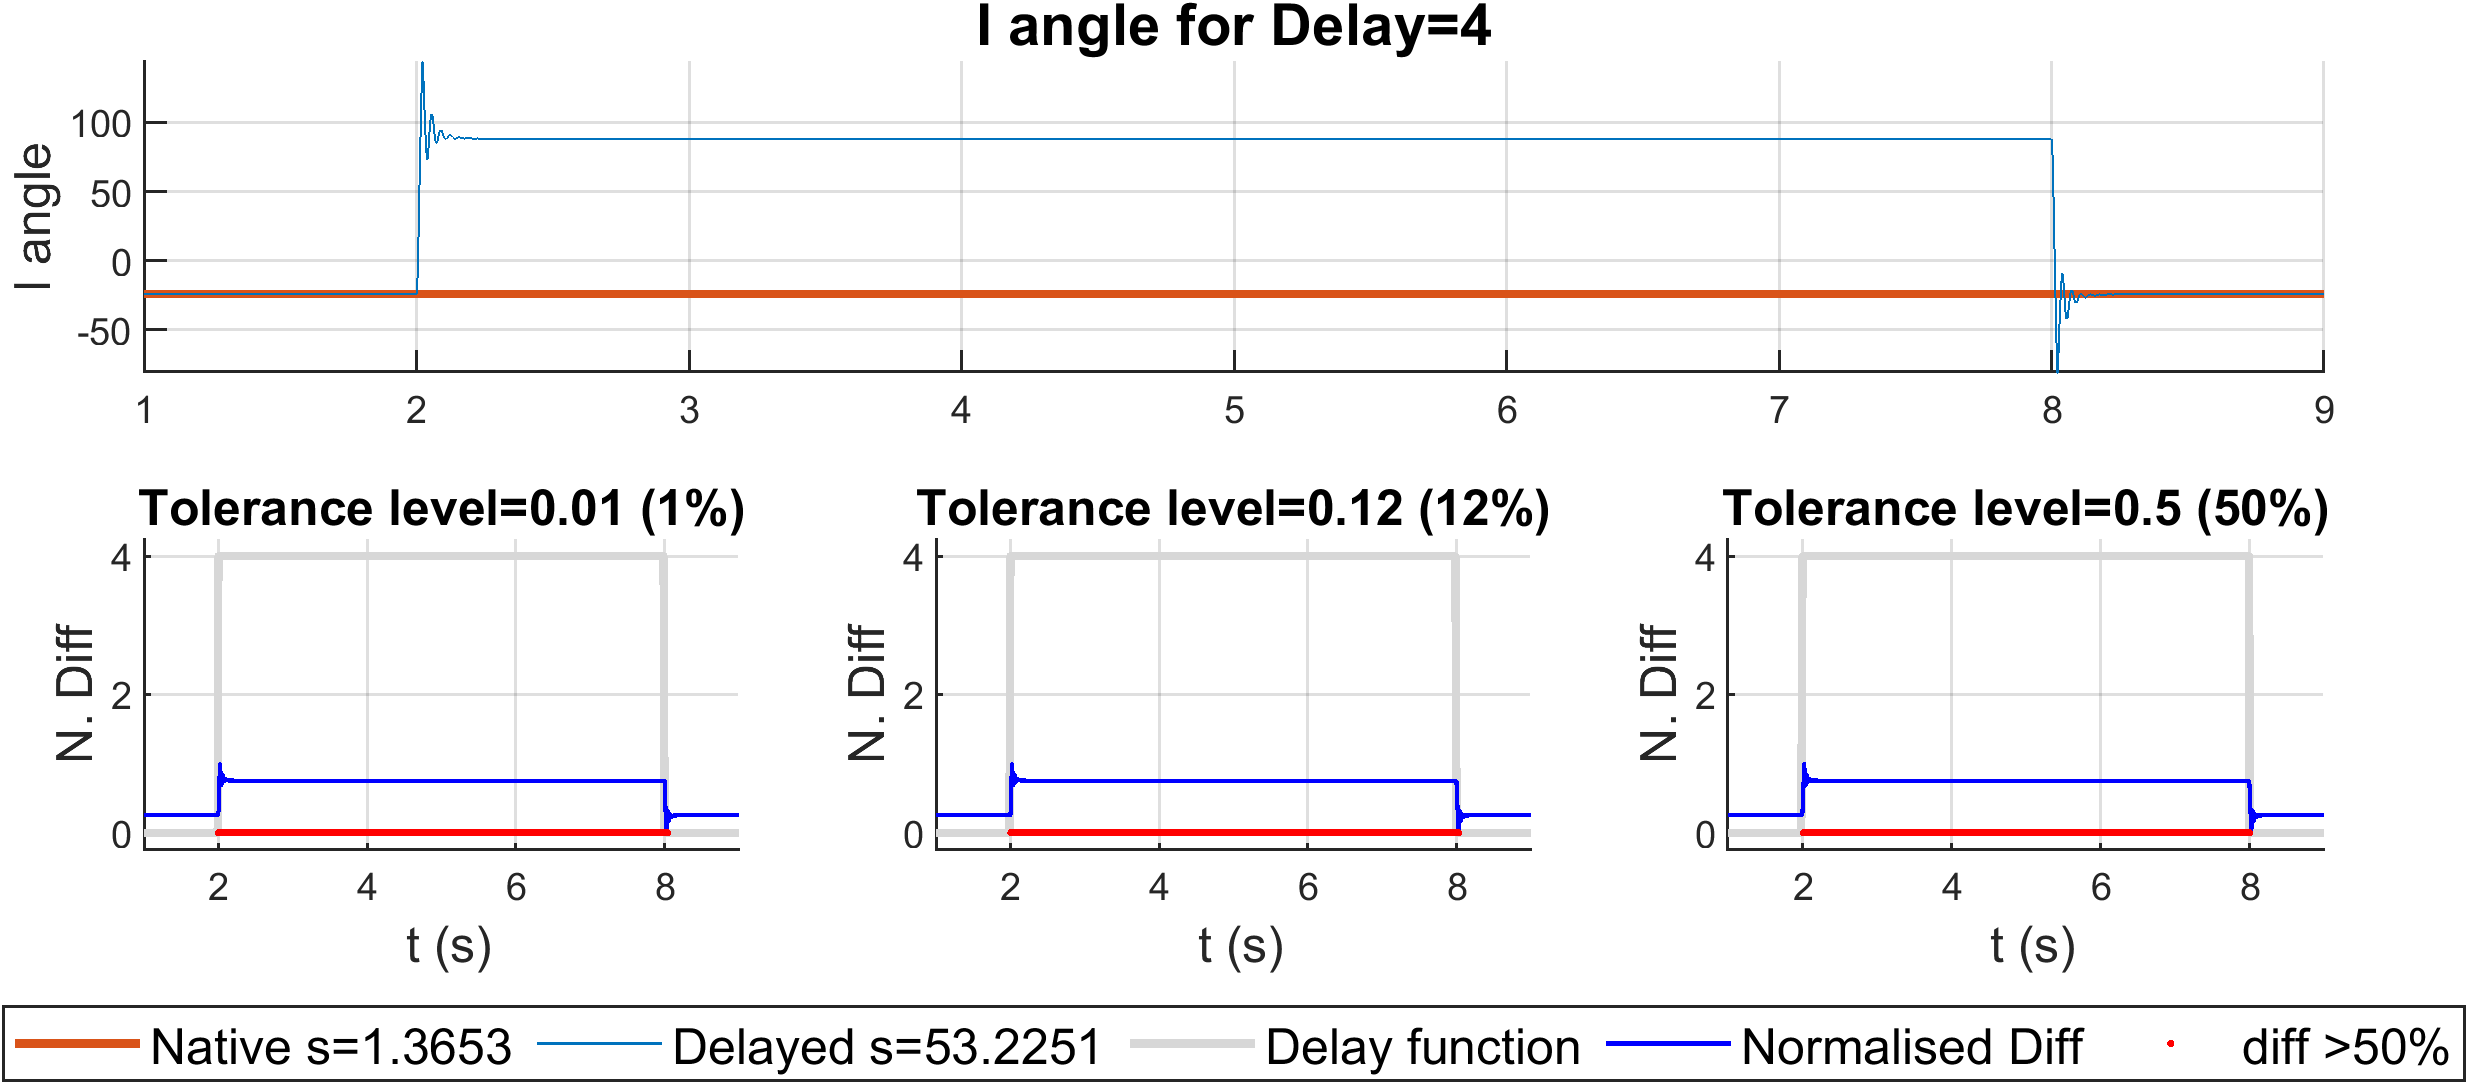
\includegraphics[width=0.95\textwidth]{PMUsim-figures/DelayOf_4/Instant_iAngle.png}}\
 \label{fig:PMUsim_Four_Angle}
 %\caption{Instant Delay Angle Output for the Delay Level of Four}
  \end{tabular}
 \end{table}
 
\newpage \subsection{Delay Level of Five}


\begin{table}[]
\caption{Results for Magnitude Output}
   \fbox{     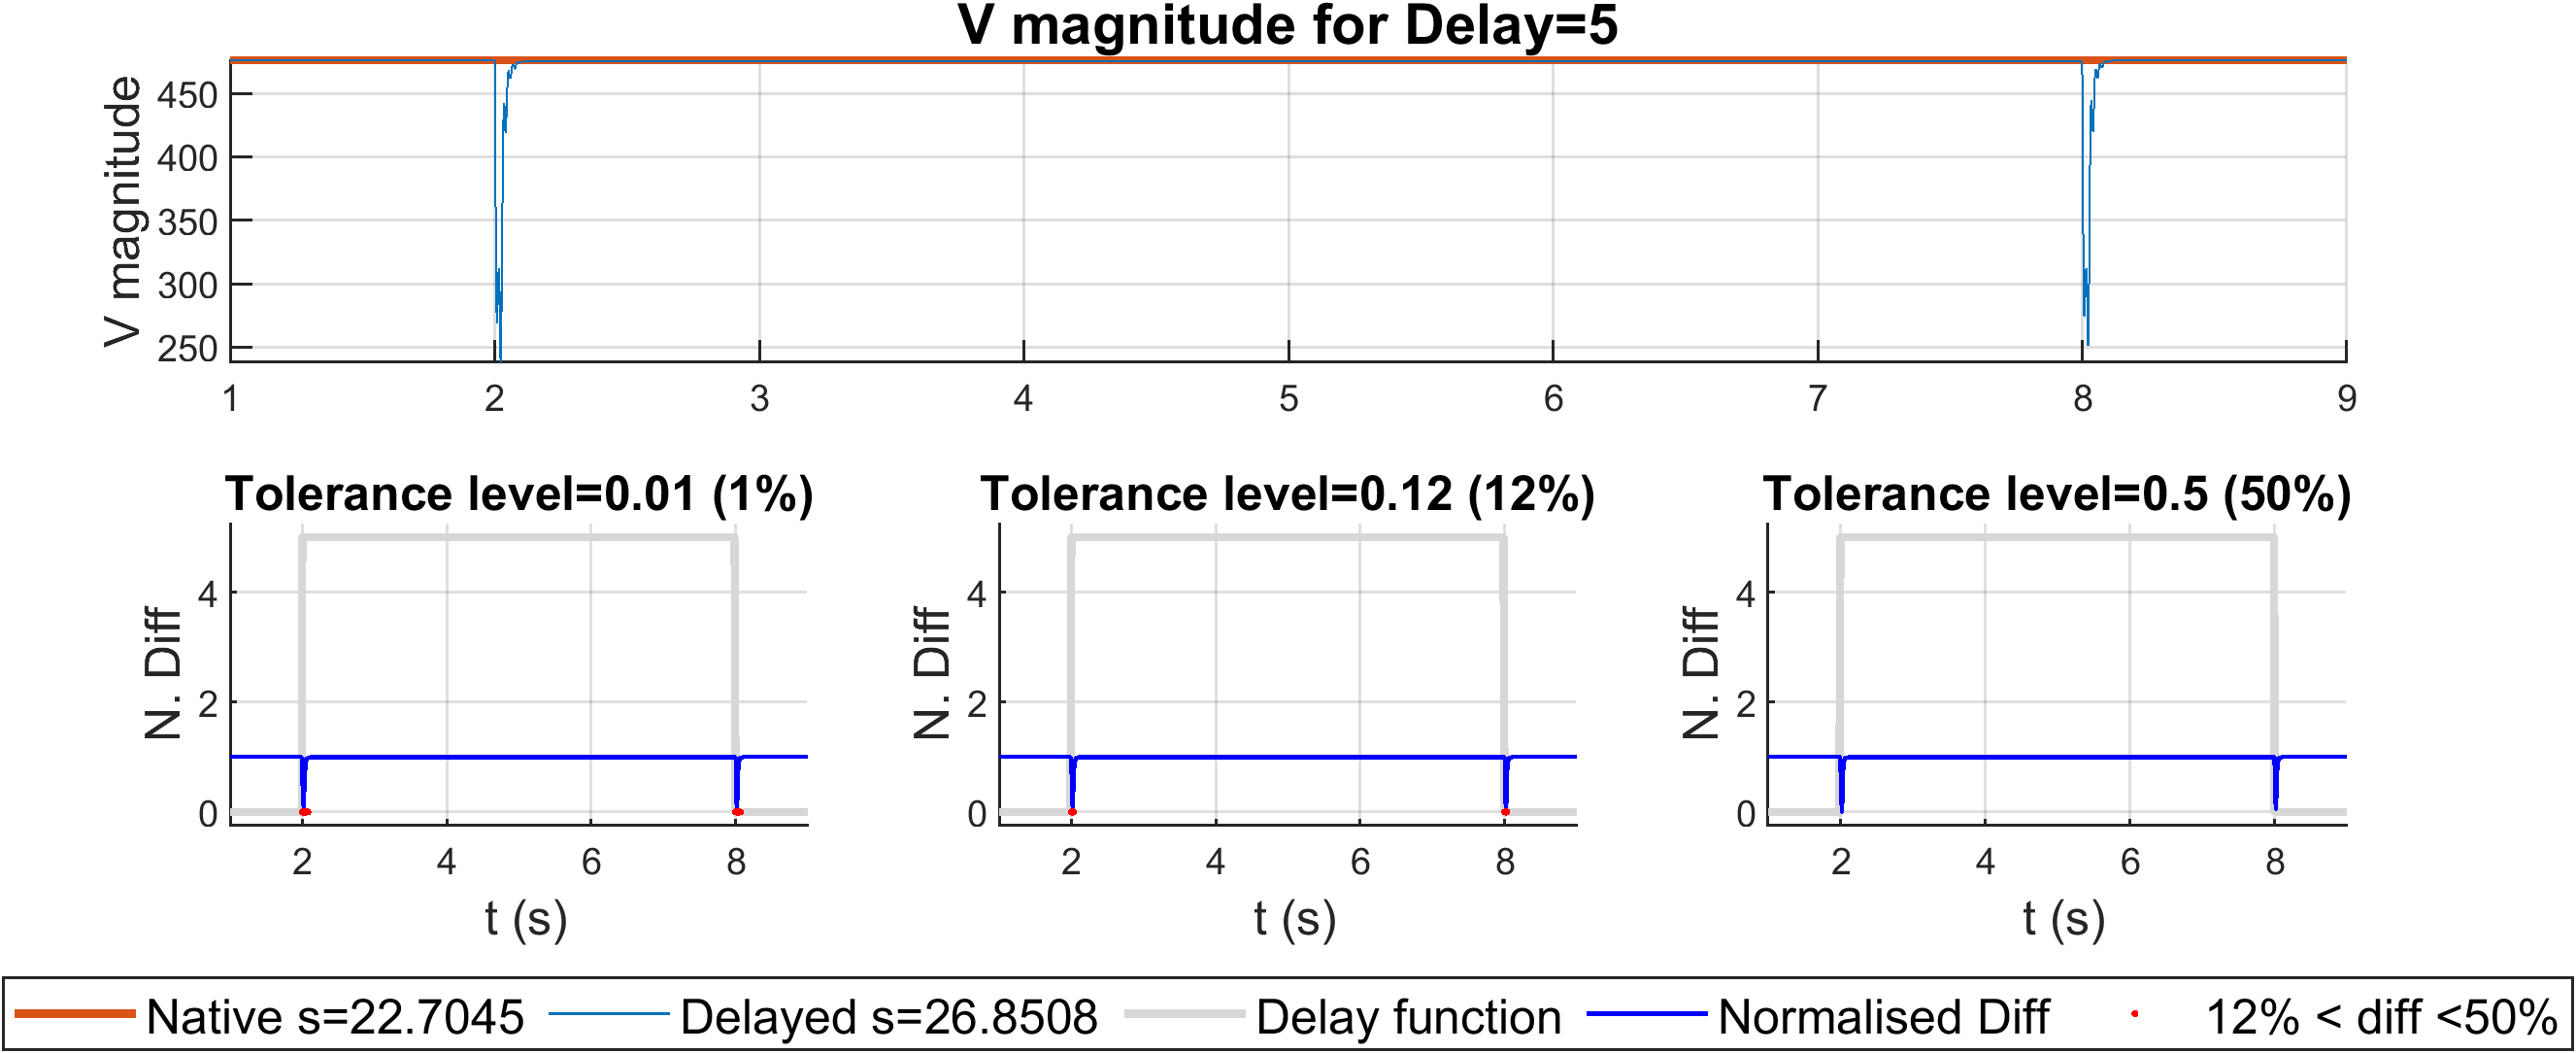
\includegraphics[width=0.95\textwidth]{PMUsim-figures/DelayOf_5/Instant_vMagnitude.png}}\
  
    
   \fbox{   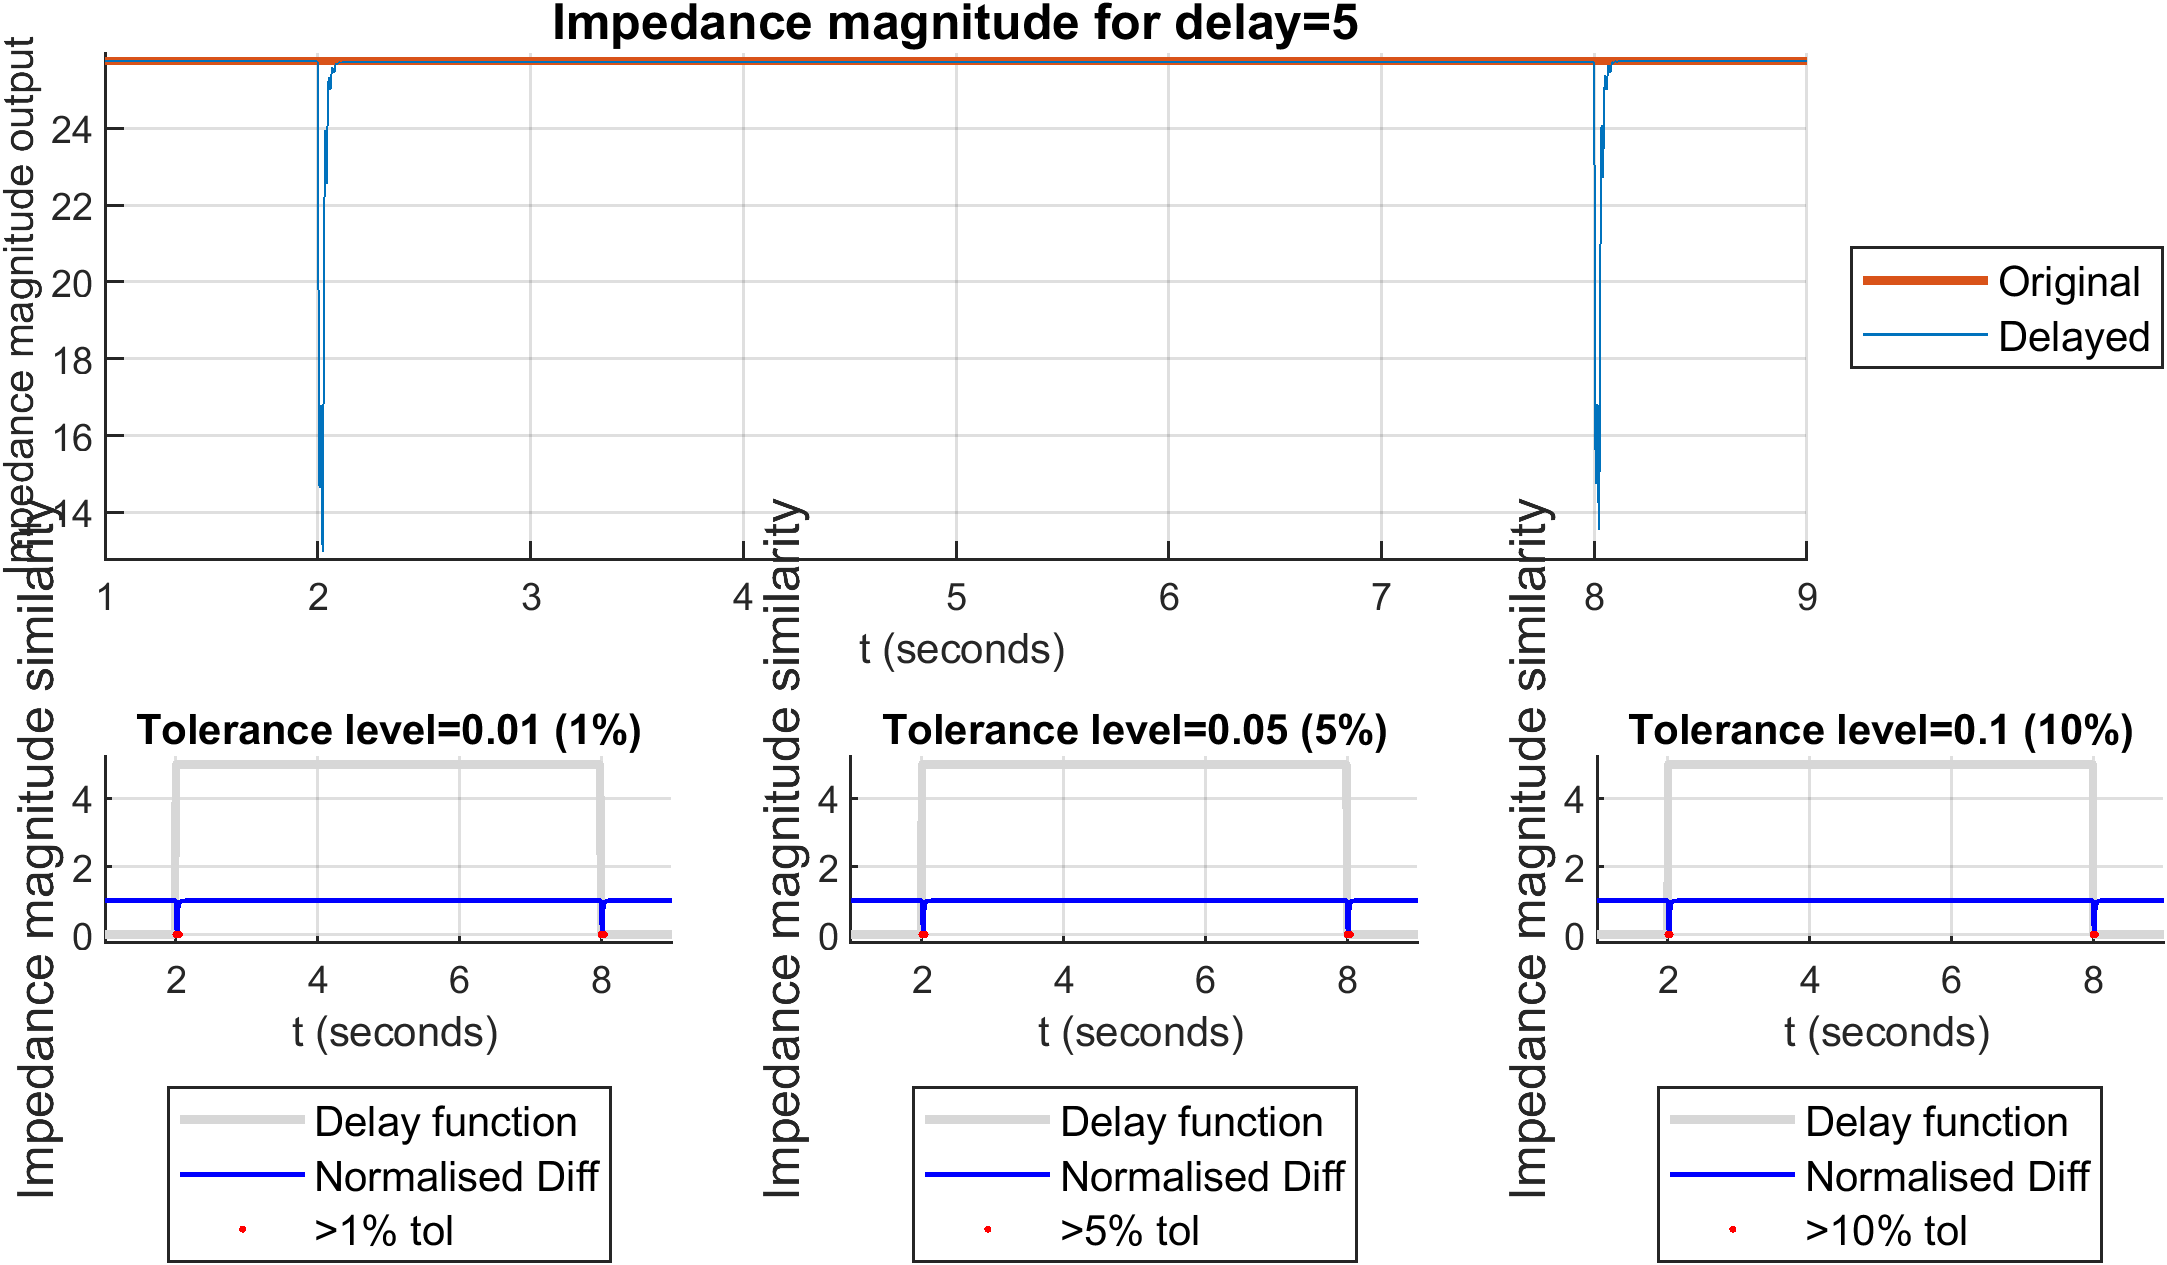
\includegraphics[width=0.95\textwidth]{PMUsim-figures/DelayOf_5/Instant_iMagnitude.png}}\
 \label{fig:PMUsim_Five_Magnitude}
 %\caption{Instant Delay Magnitude Output for the Delay Level of Five}
  \end{tabular}
 \end{table}
 
 
\newpage  

\begin{table}[]
\caption{Results for Frequency Output}
   \fbox{     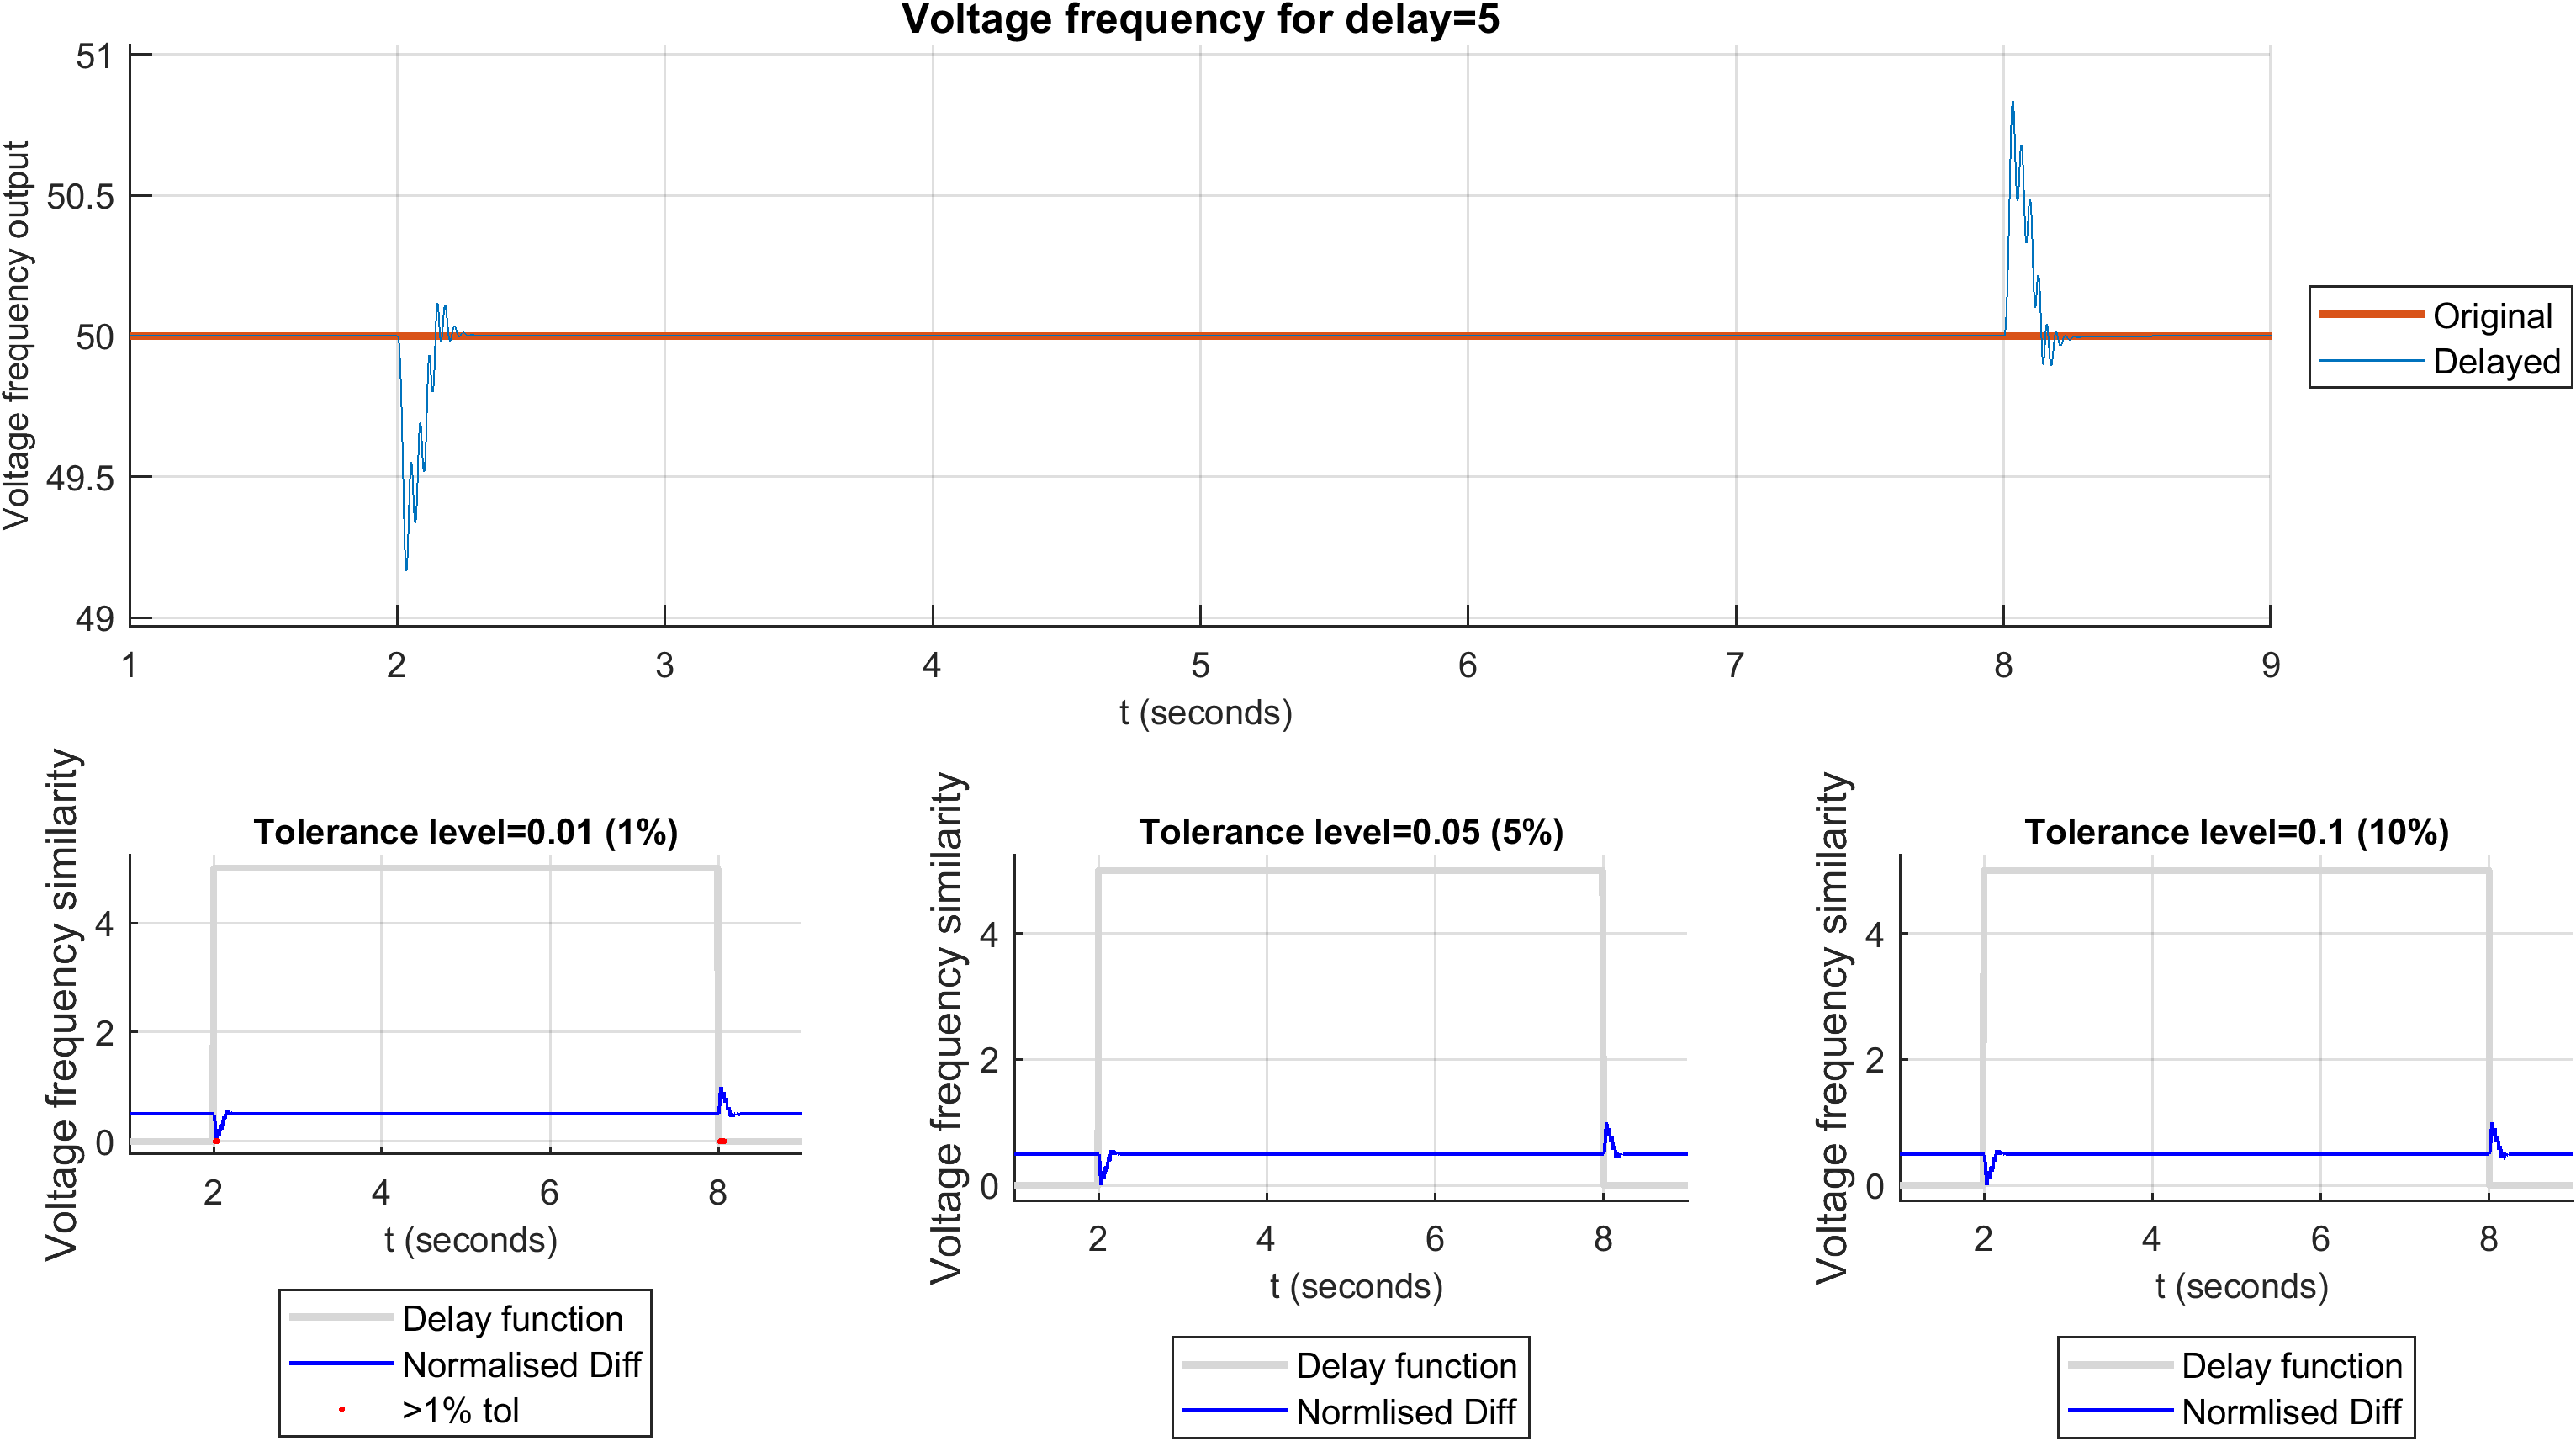
\includegraphics[width=0.95\textwidth]{PMUsim-figures/DelayOf_5/Instant_vFrequency.png}}\
  
    
   \fbox{  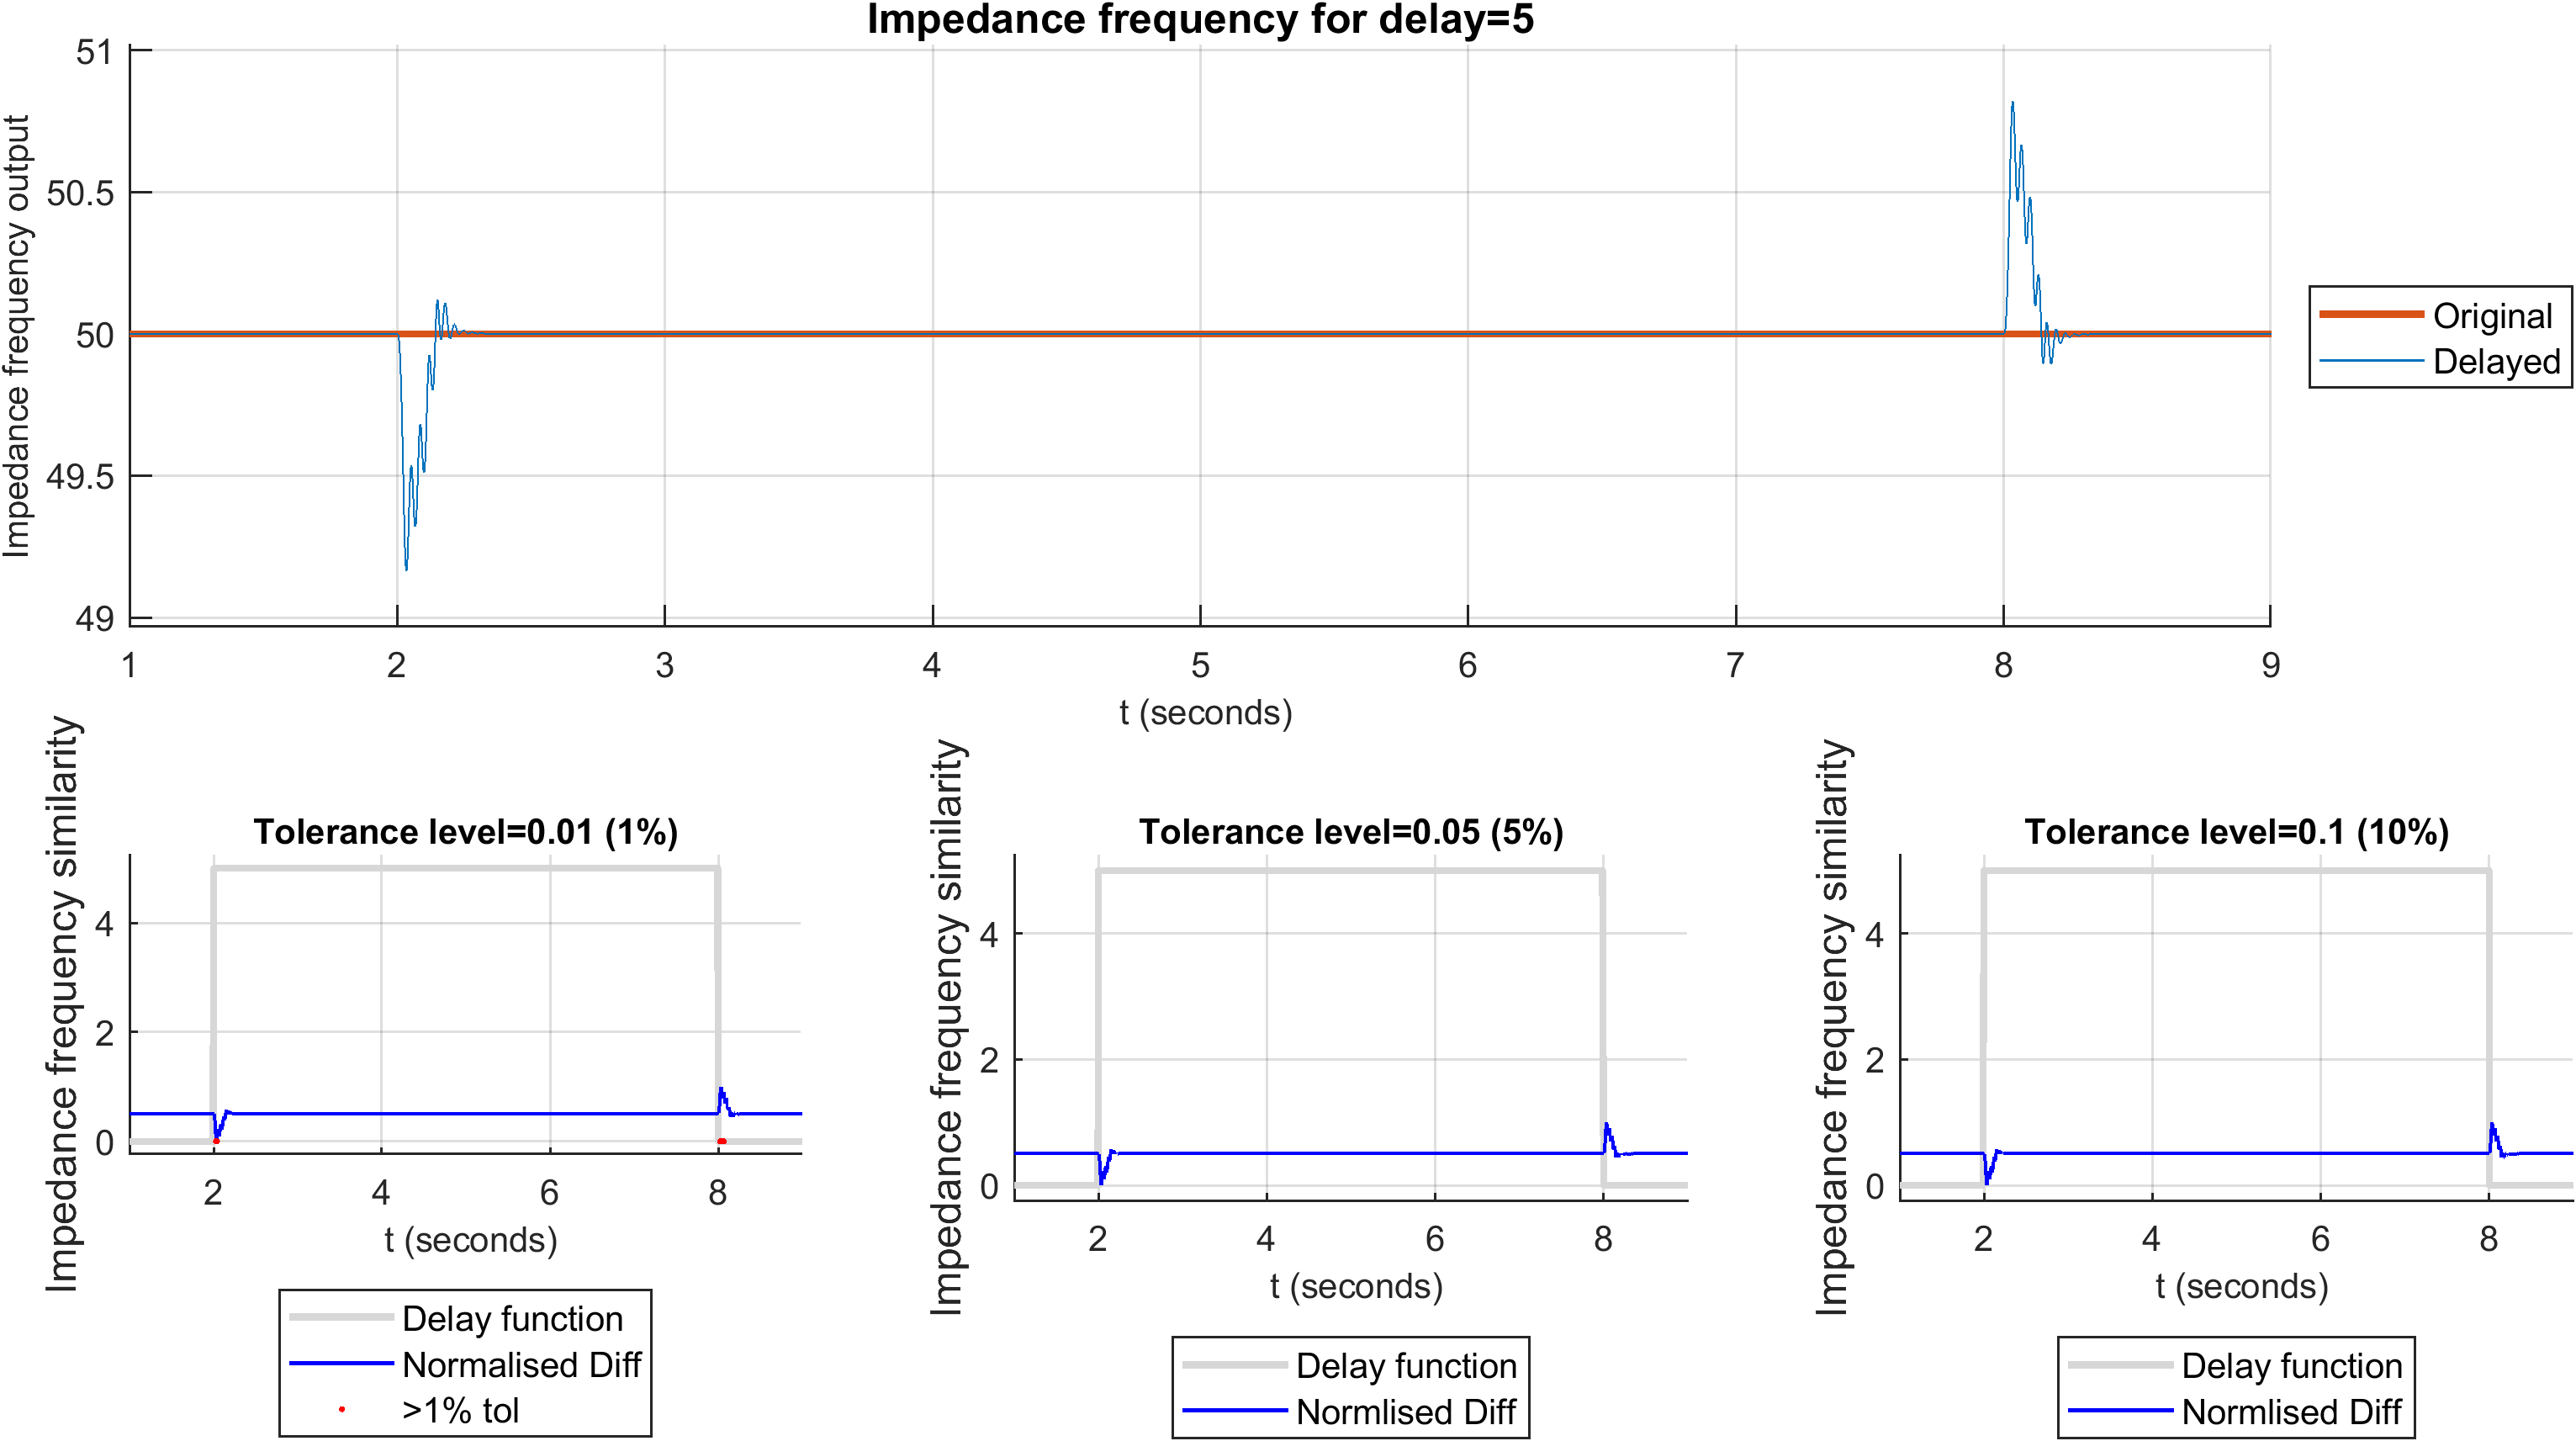
\includegraphics[width=0.95\textwidth]{PMUsim-figures/DelayOf_5/Instant_iFrequency.png}}\
 \label{fig:PMUsim_Five_Frequency}
 %\caption{Instant Delay Frequency Output for the Delay Level of Five}
  \end{tabular}
 \end{table}
  

\newpage 

\begin{table}[]
\caption{Results for Angle Output}
   \fbox{     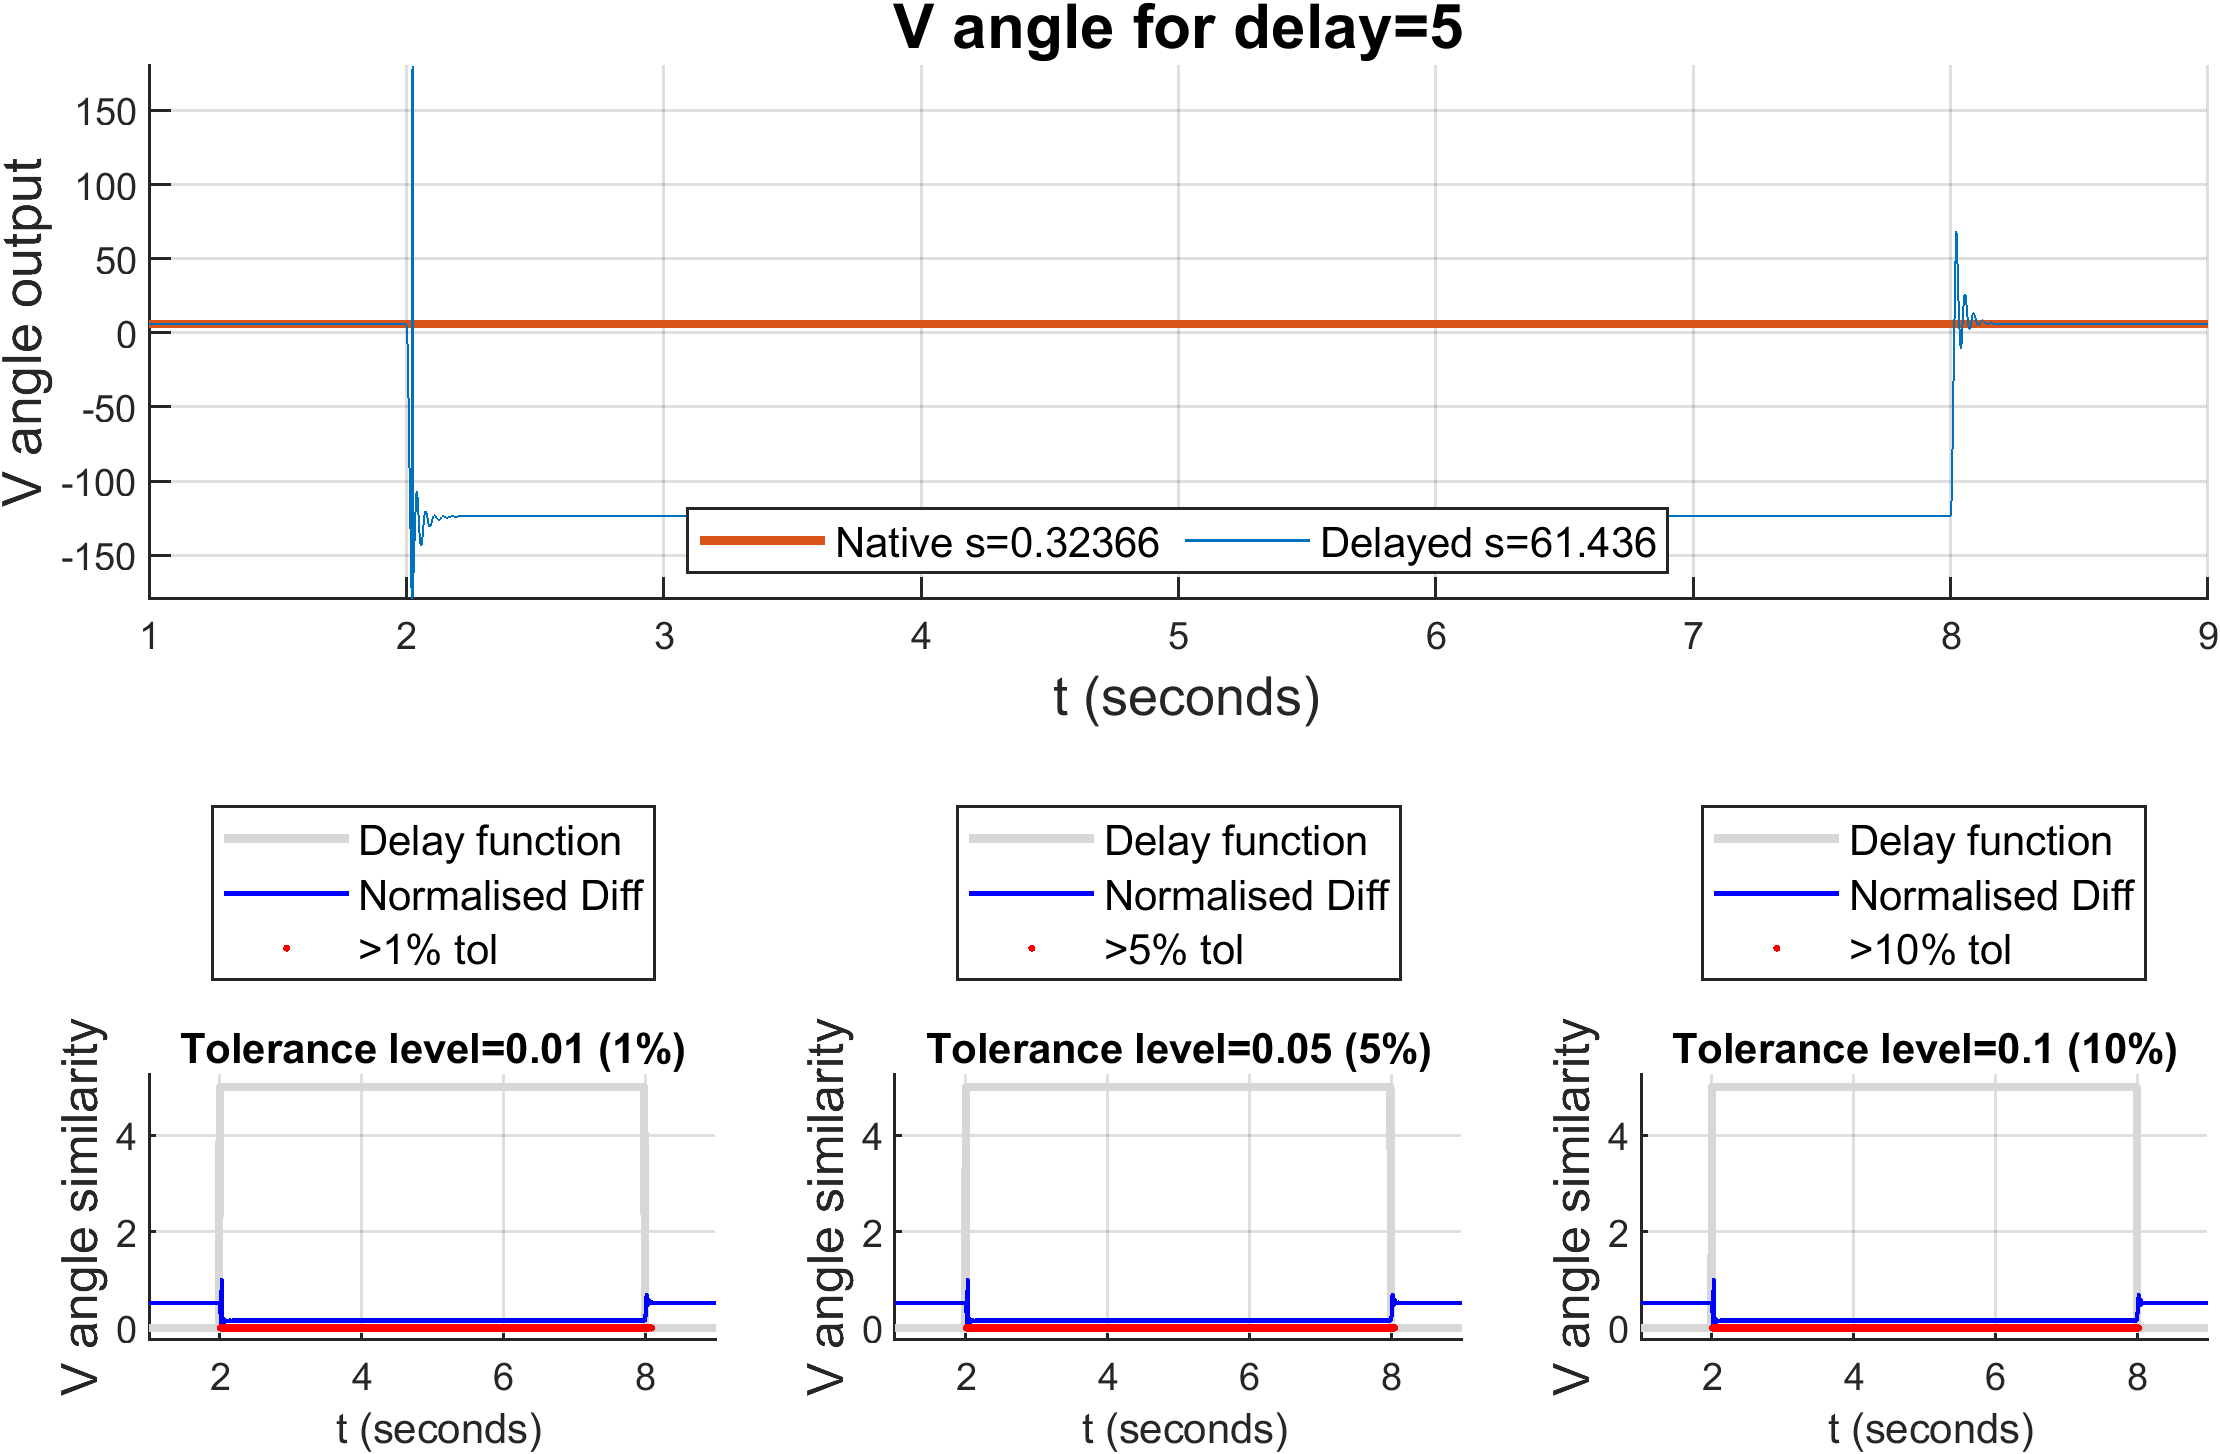
\includegraphics[width=0.95\textwidth]{PMUsim-figures/DelayOf_5/Instant_vAngle.png}}\
  
    
   \fbox{  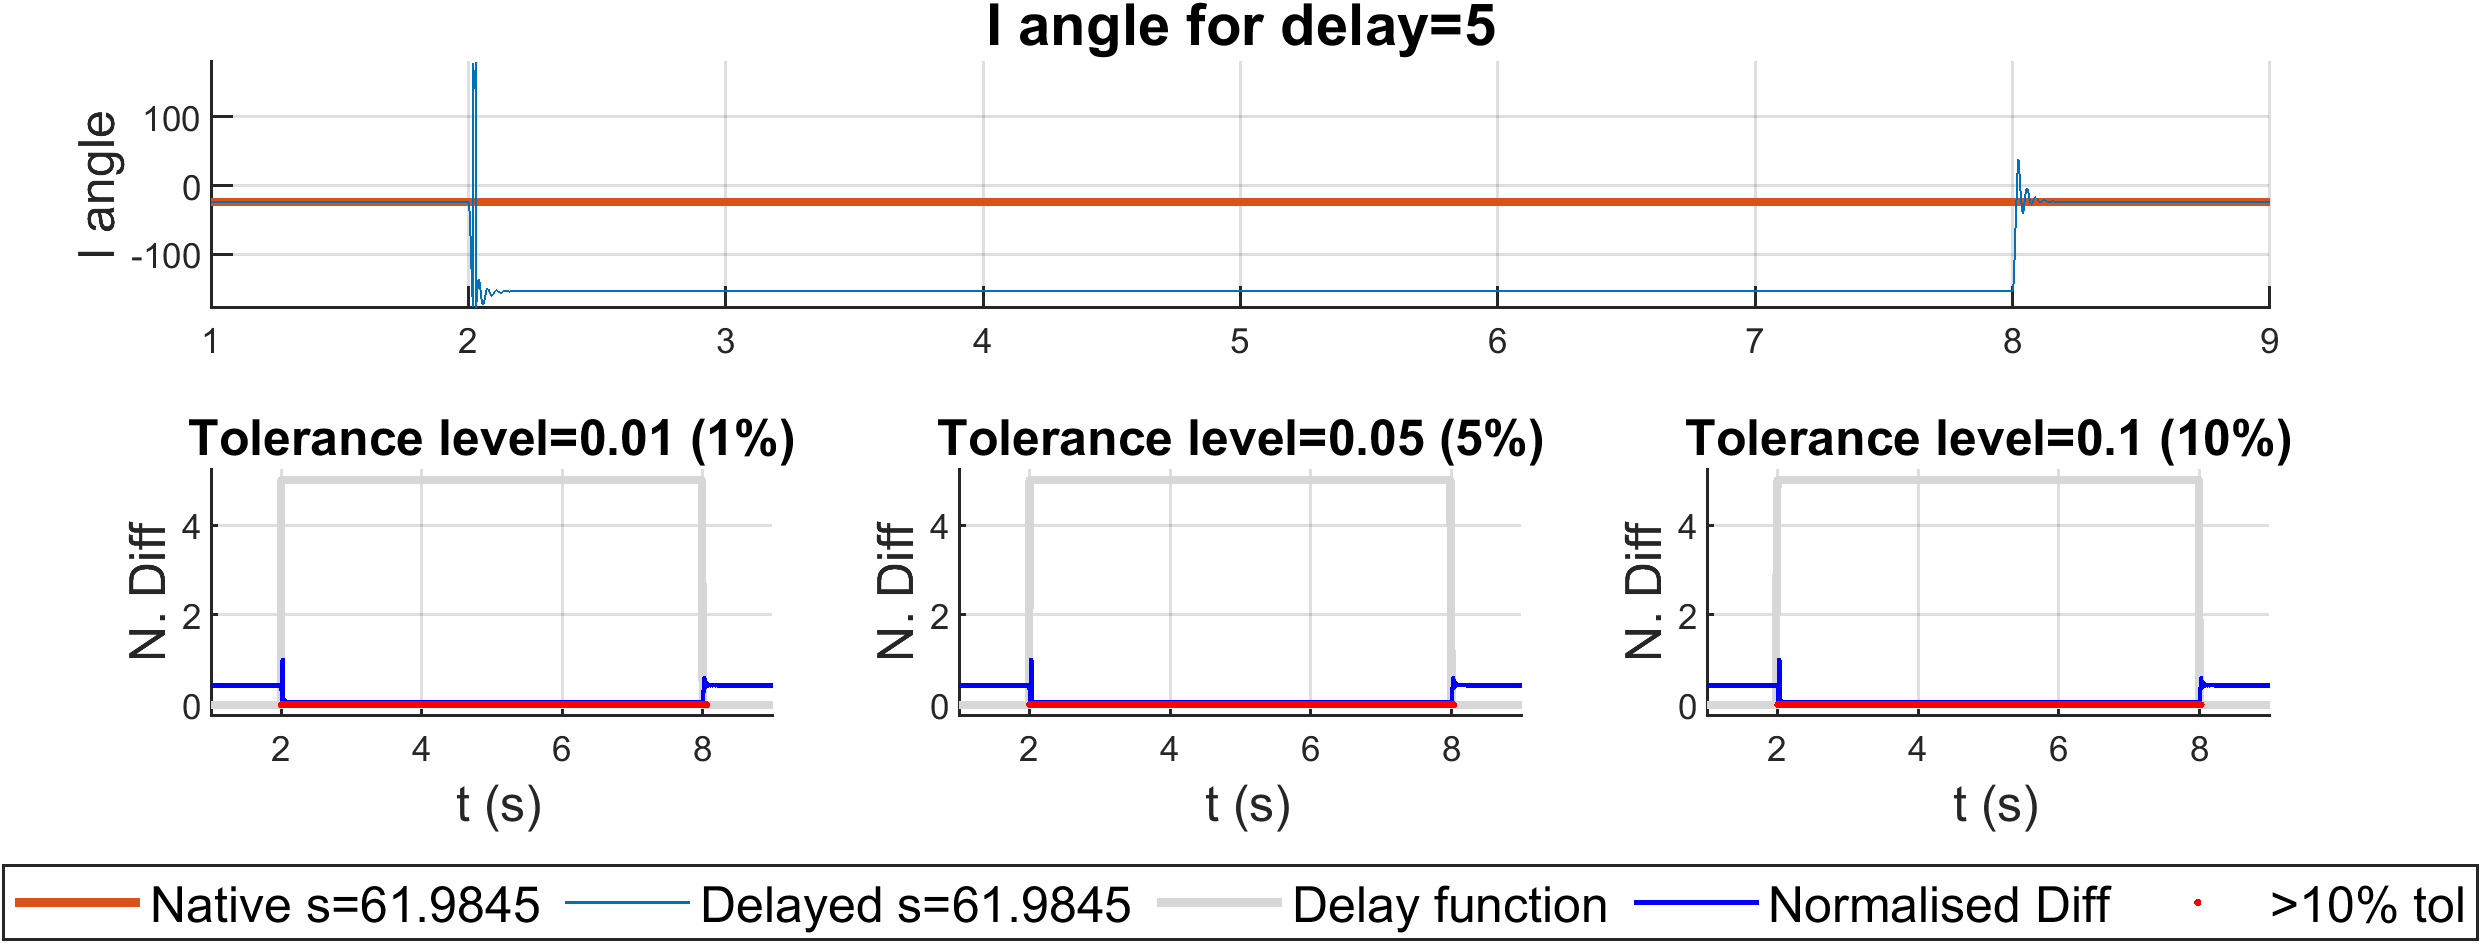
\includegraphics[width=0.95\textwidth]{PMUsim-figures/DelayOf_5/Instant_iAngle.png}}\
 \label{fig:PMUsim_Five_Angle}
 %\caption{Instant Delay Angle Output for the Delay Level of Five}
  \end{tabular}
 \end{table}
 

\newpage \subsection{Delay Level of Six}


\begin{table}[]
\caption{Results for Magnitude Output}
   \fbox{    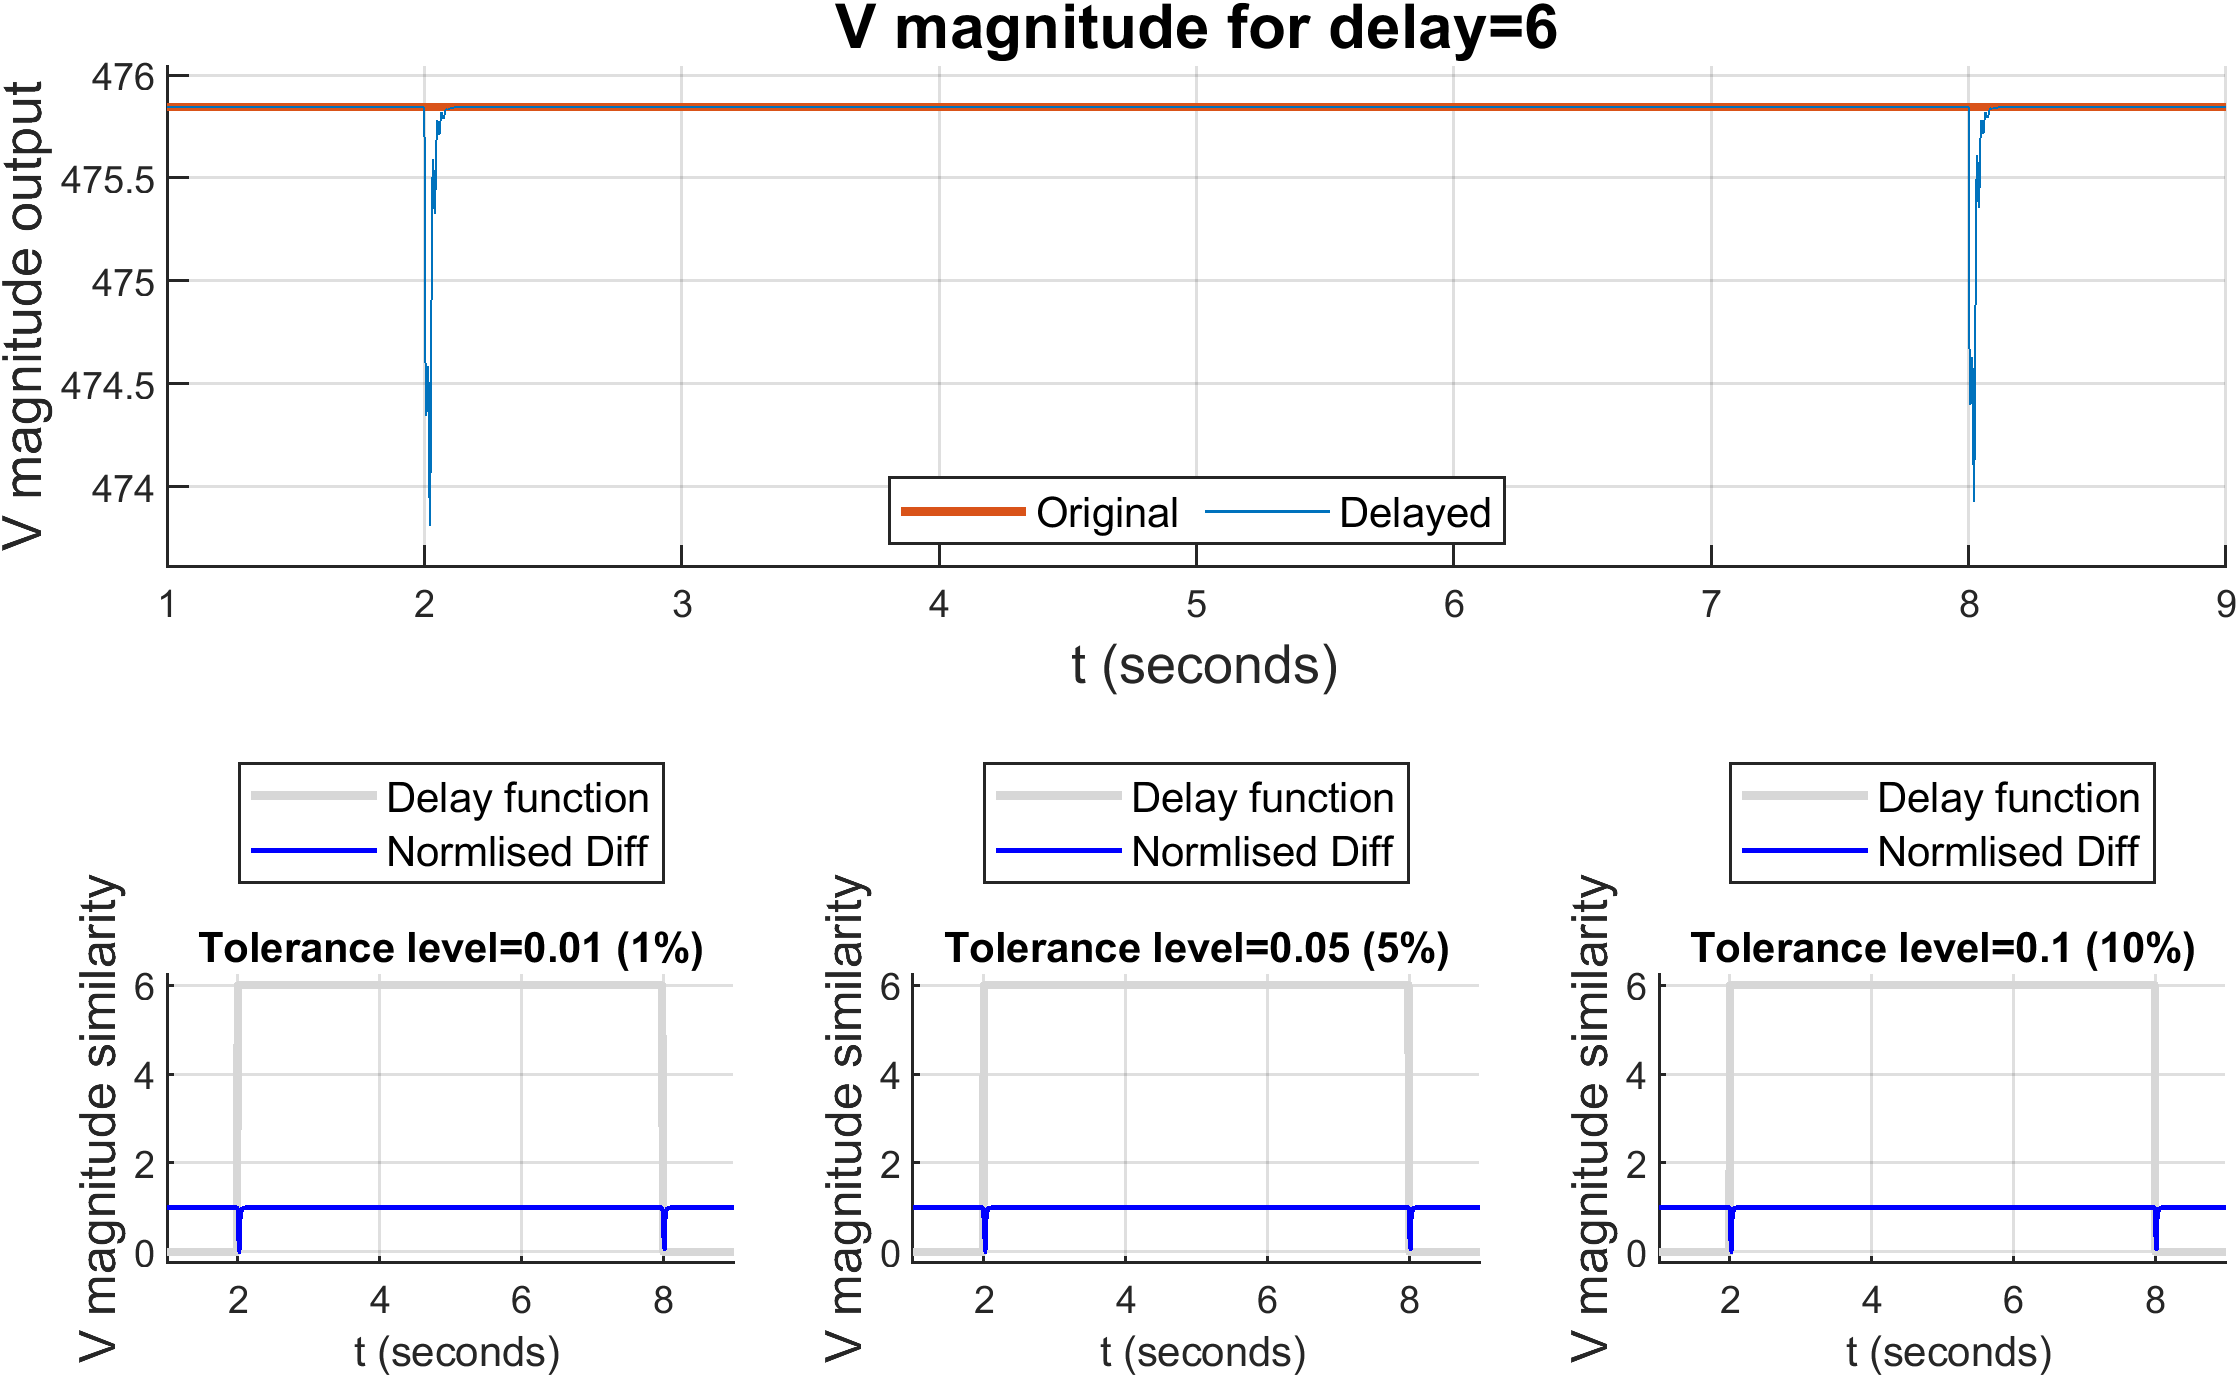
\includegraphics[width=0.95\textwidth]{PMUsim-figures/DelayOf_6/Instant_vMagnitude.png}}\
  
    
   \fbox{    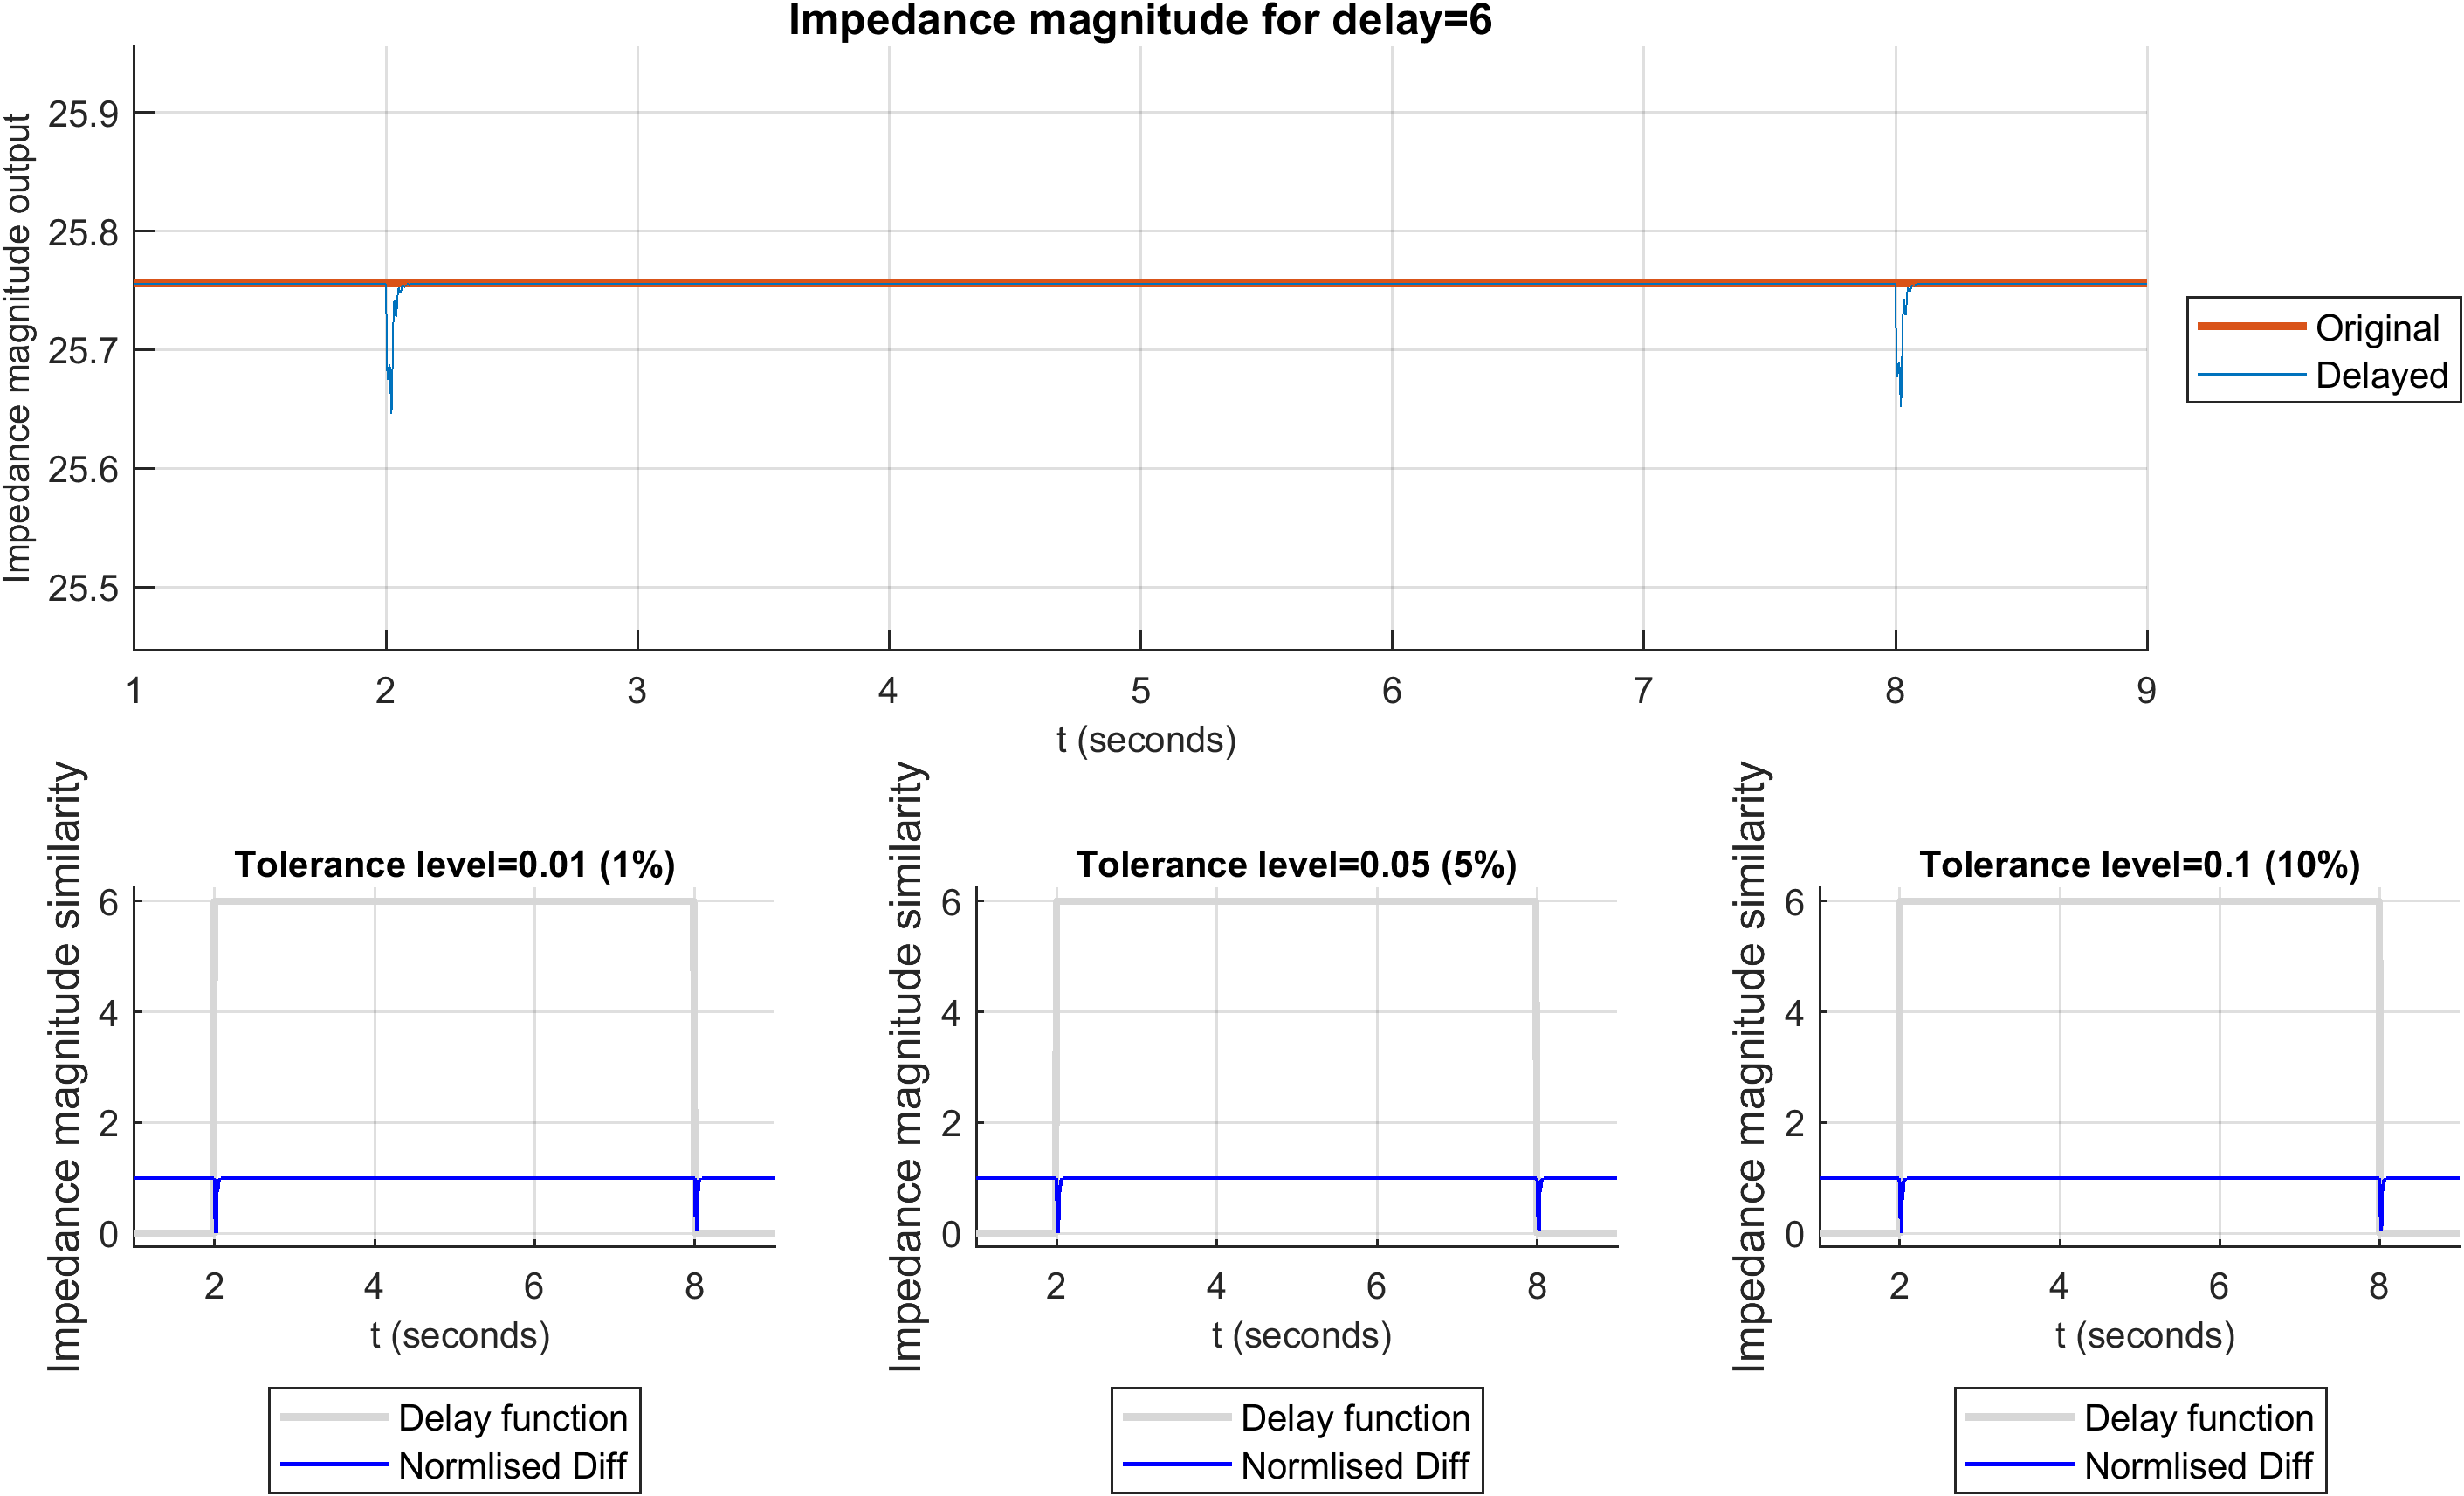
\includegraphics[width=0.95\textwidth]{PMUsim-figures/DelayOf_6/Instant_iMagnitude.png}}\  
 \label{fig:PMUsim_Six_Magnitude}
 %\caption{Instant Delay Magnitude Output for the Delay Level of Six}
  \end{tabular}
 \end{table}

\newpage  

\begin{table}[]
\caption{Results for Frequency Output}
   \fbox{     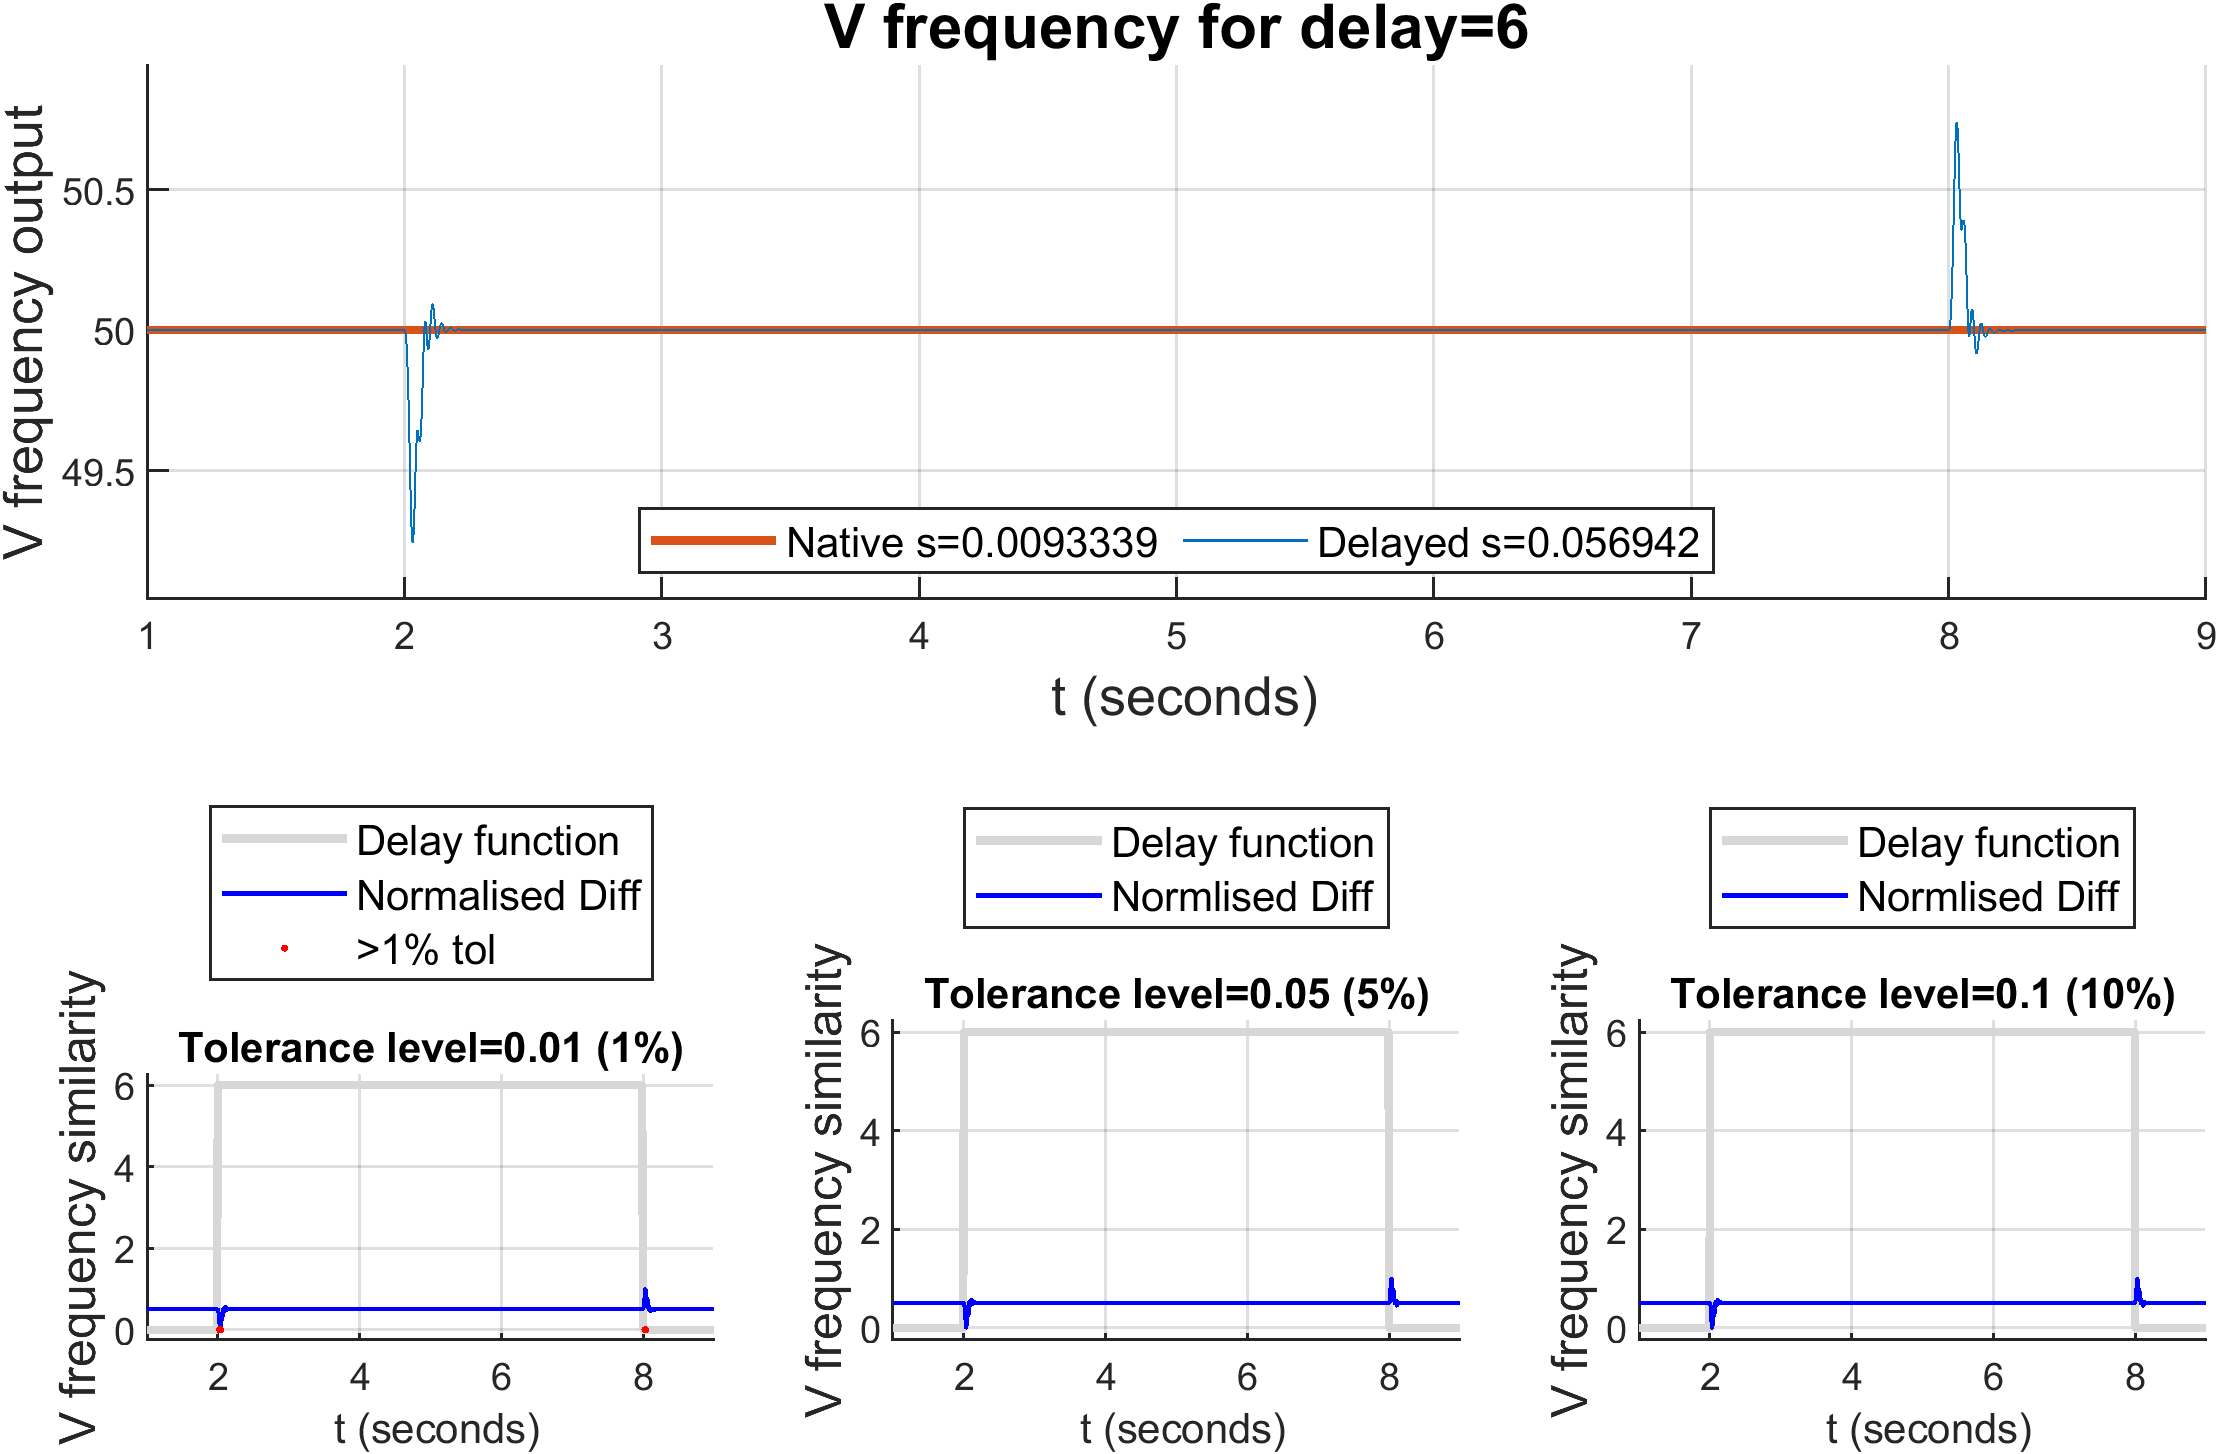
\includegraphics[width=0.95\textwidth]{PMUsim-figures/DelayOf_6/Instant_vFrequency.png}}\
  
    
   \fbox{  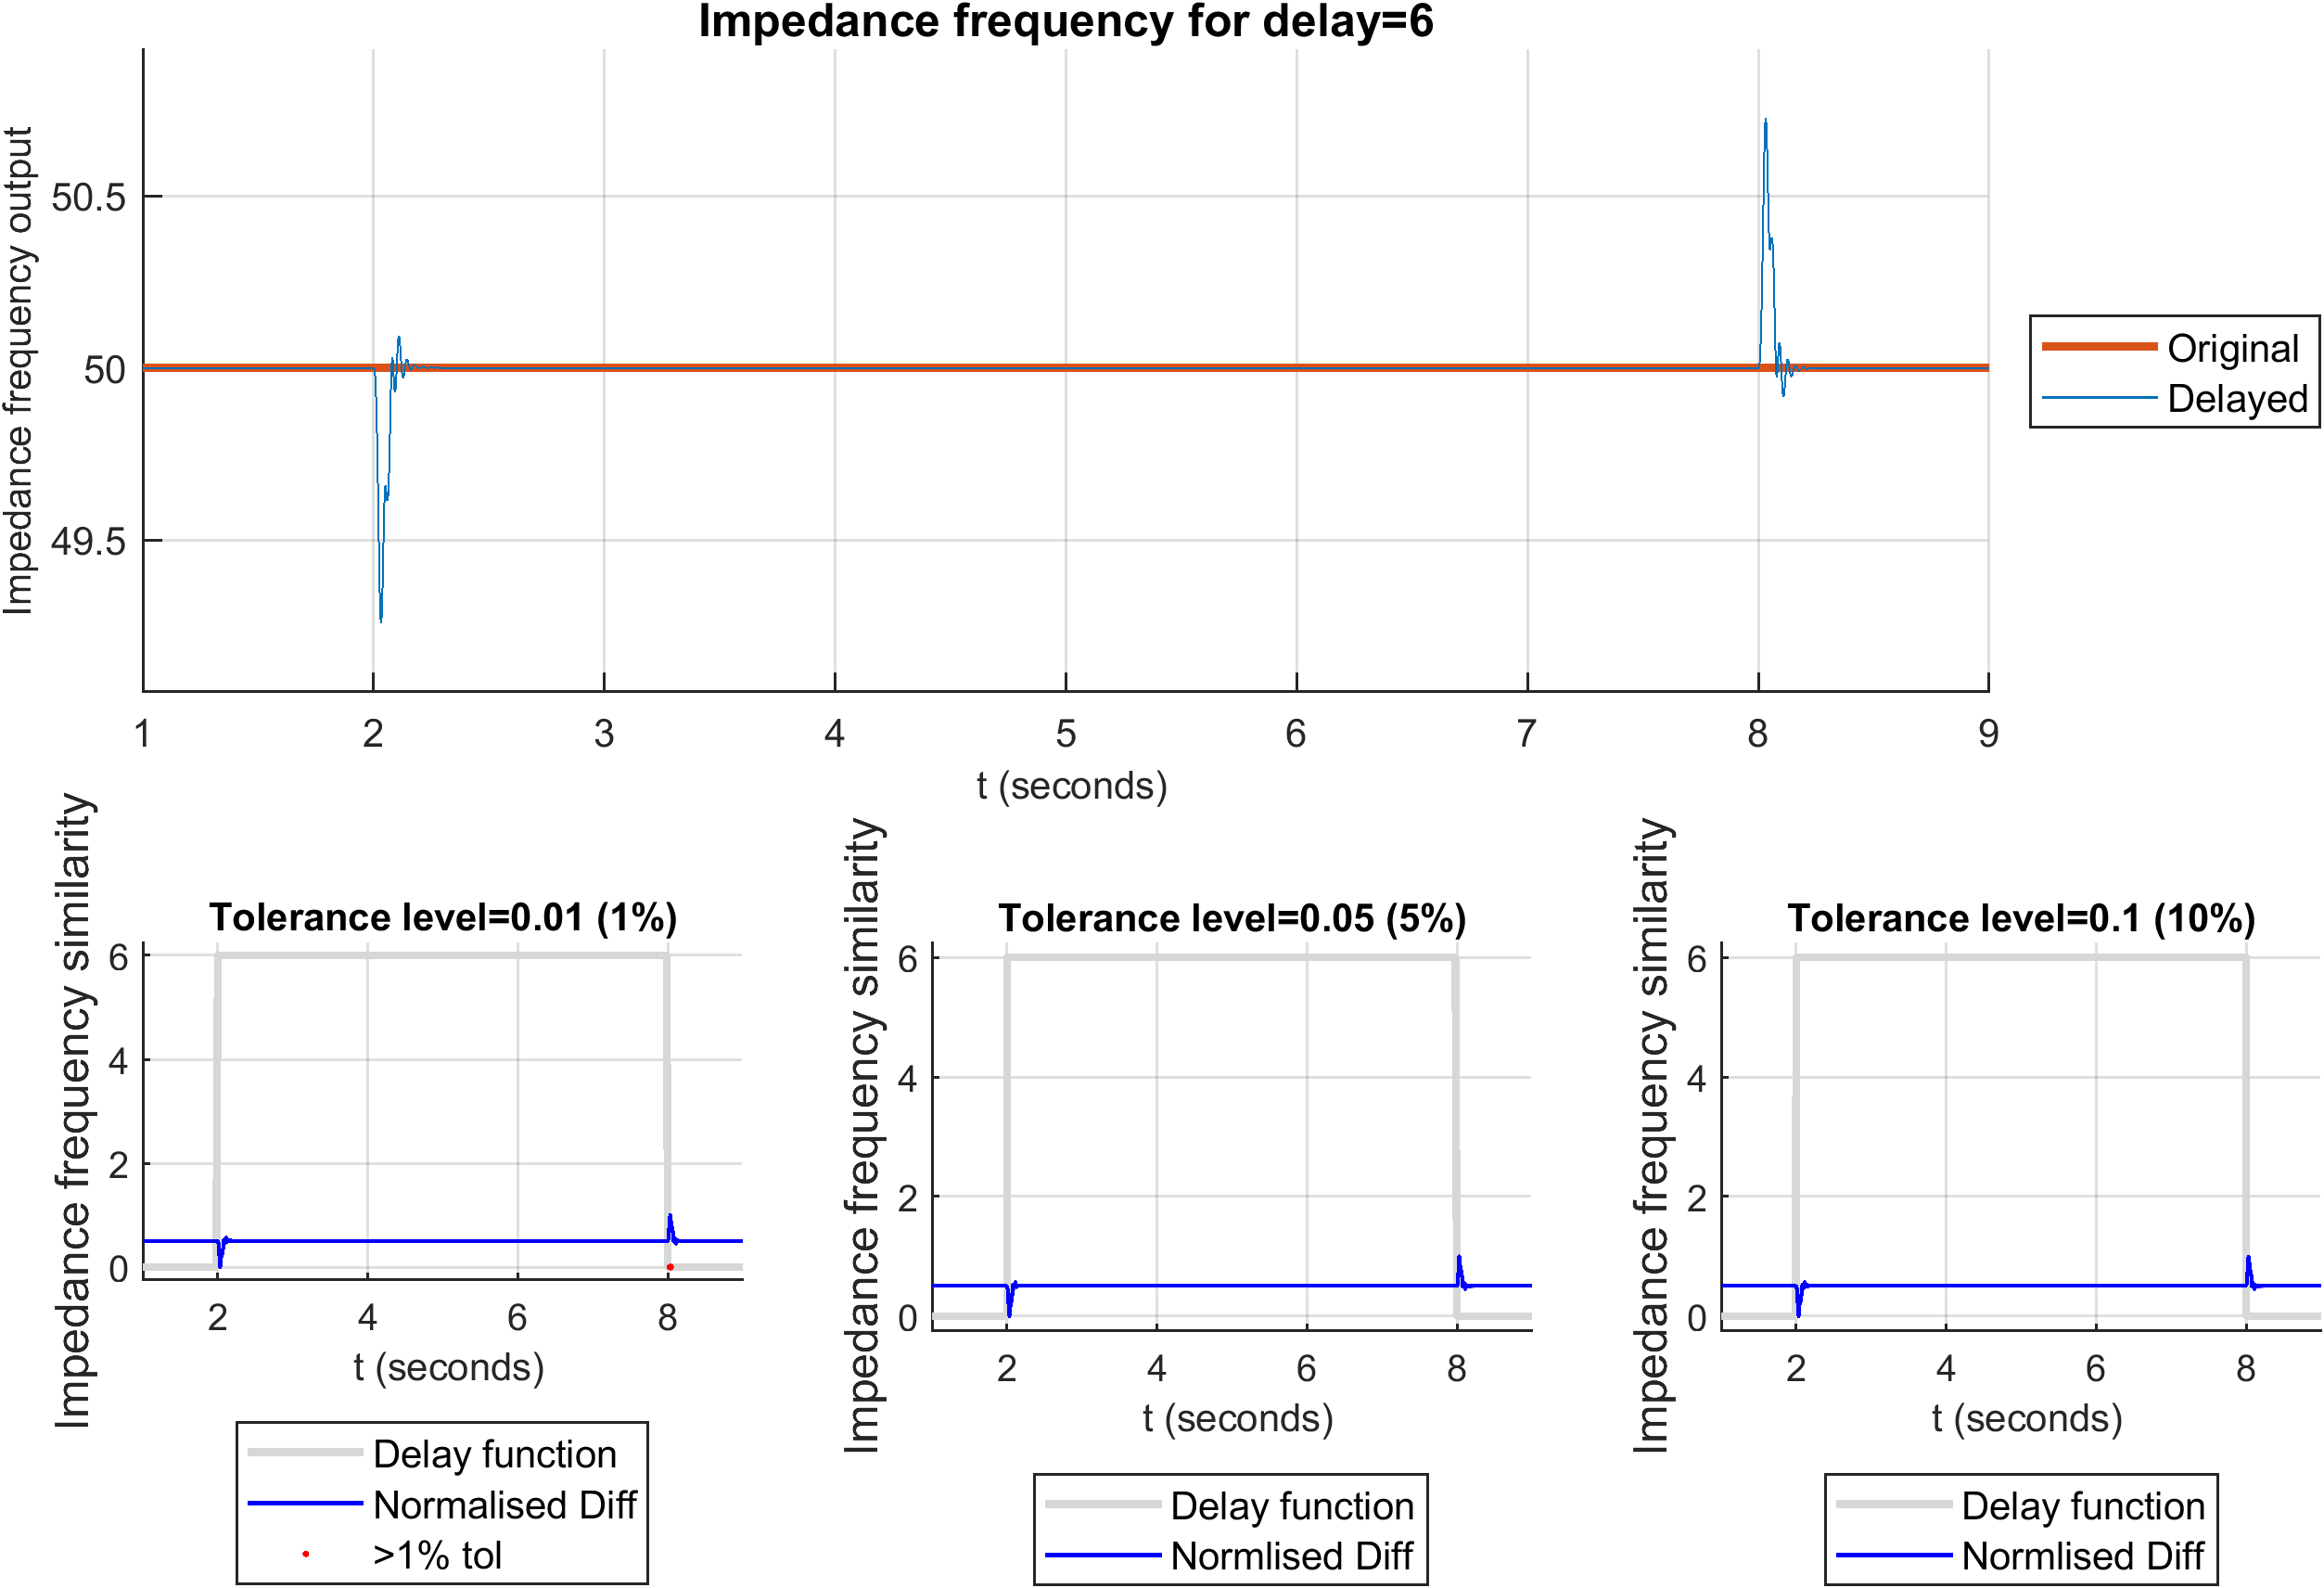
\includegraphics[width=0.95\textwidth]{PMUsim-figures/DelayOf_6/Instant_iFrequency.png}}\ 
 \label{fig:PMUsim_Six_Frequency}
 %\caption{Instant Delay Frequency Output for the Delay Level of Six}
  \end{tabular}
 \end{table}
   


\newpage 

\begin{table}[]
\caption{Results for Angle Output}
   \fbox{     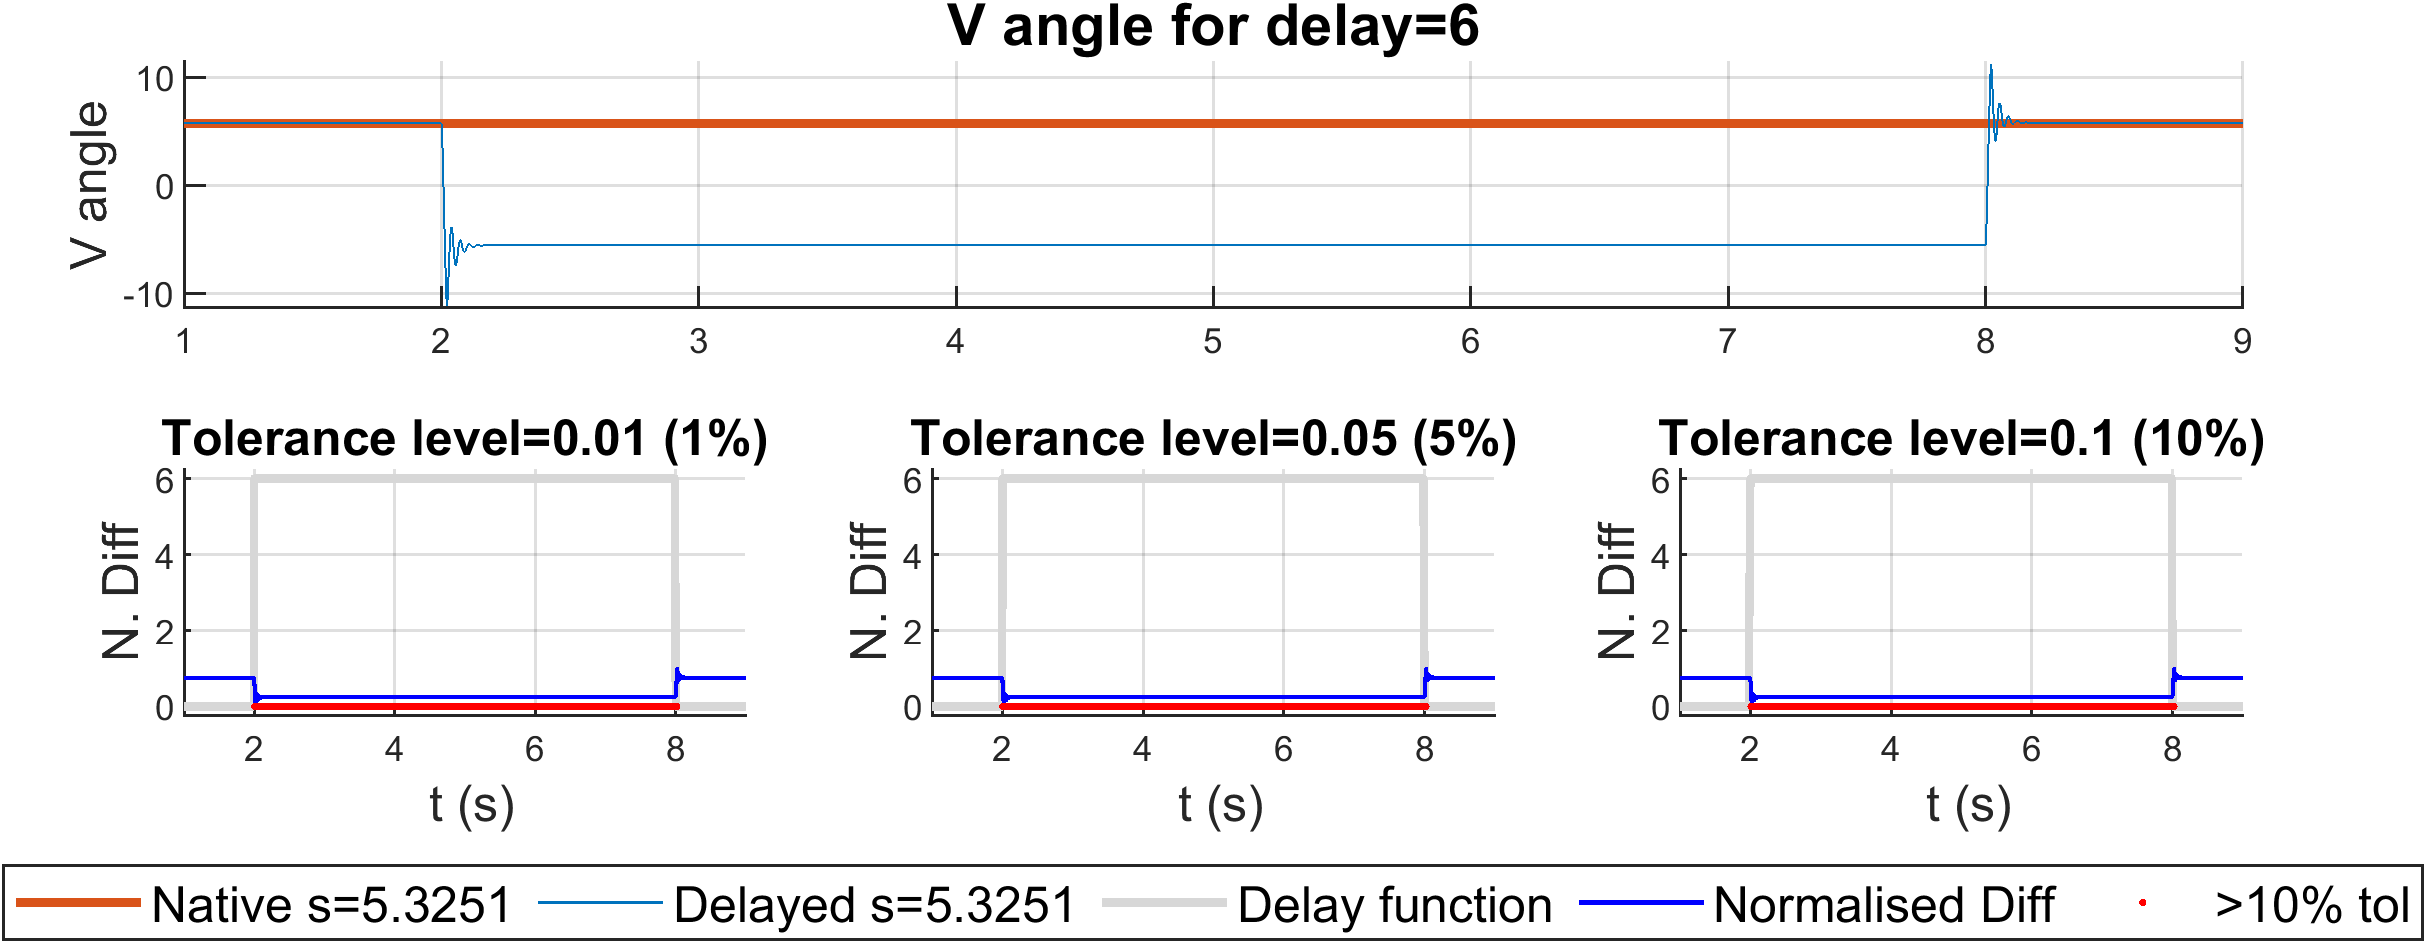
\includegraphics[width=0.95\textwidth]{PMUsim-figures/DelayOf_6/Instant_vAngle.png}}\
  
    
   \fbox{  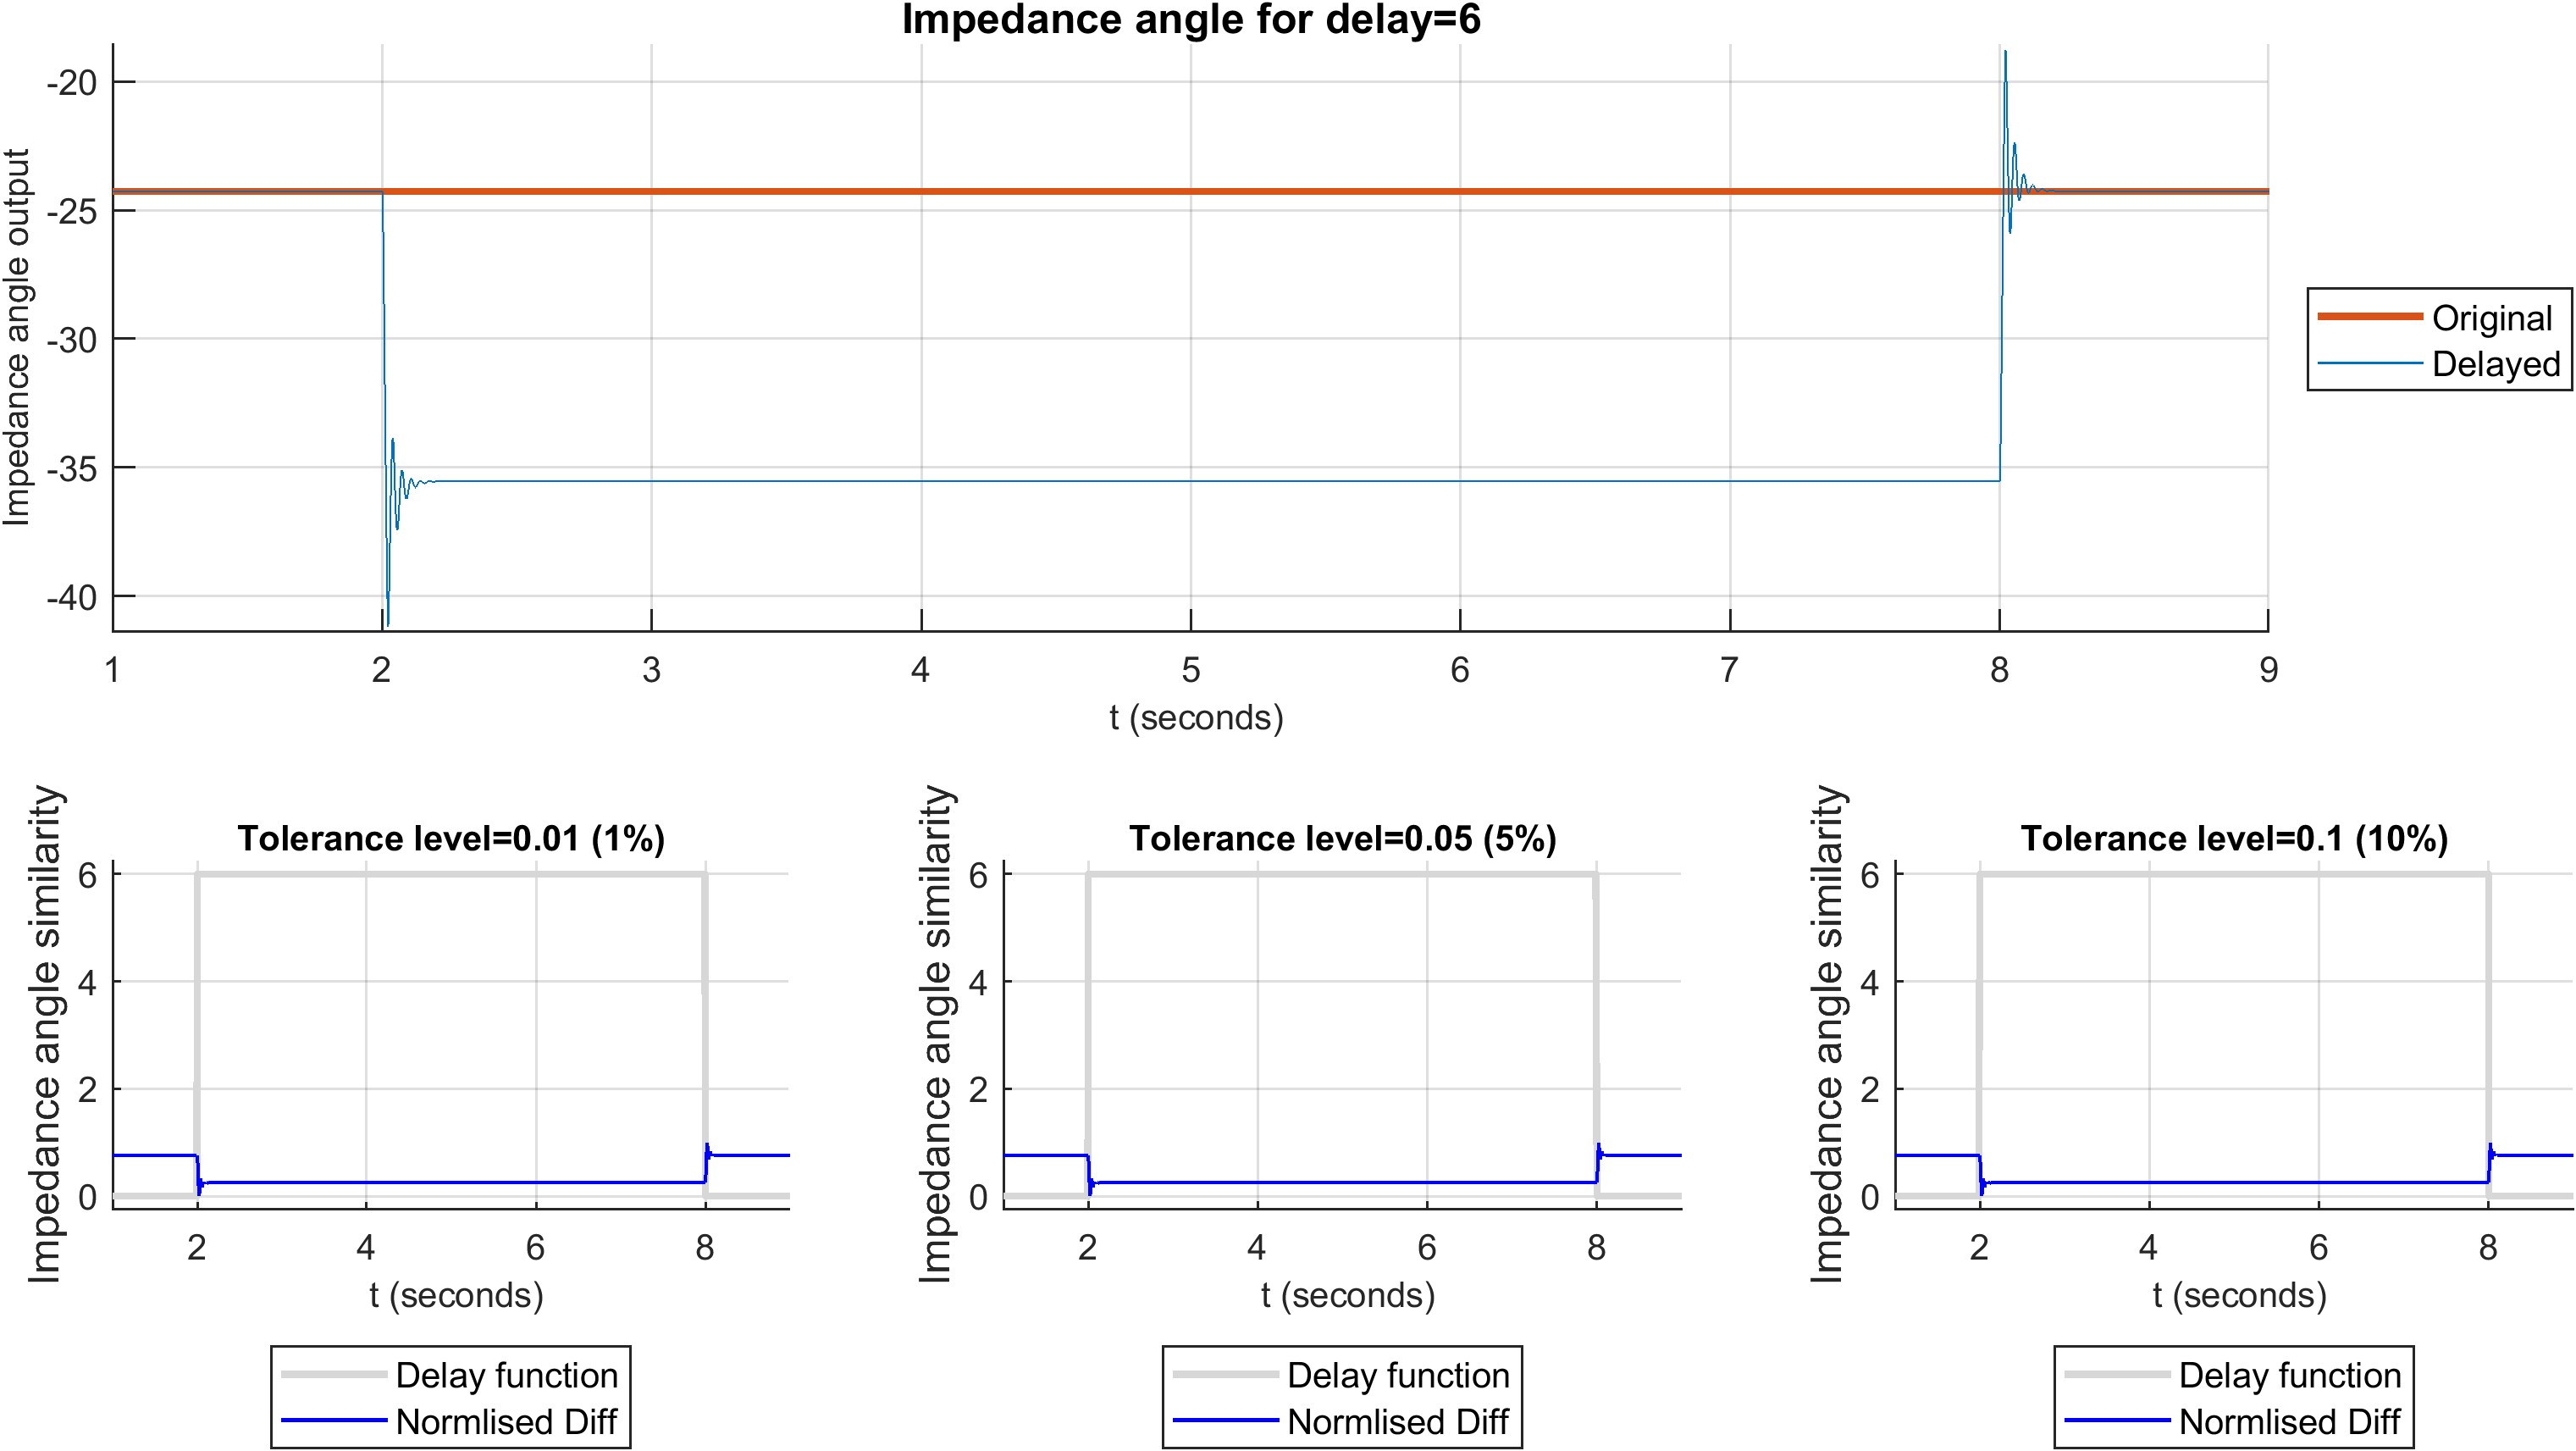
\includegraphics[width=0.95\textwidth]{PMUsim-figures/DelayOf_6/Instant_iAngle.png}}\
 \label{fig:PMUsim_Six_Angle}
 %\caption{Instant Delay Angle Output for the Delay Level of Six}
  \end{tabular}
 \end{table}
 


\section{Step-Wise Delay Functions}
\newpage \subsection{Delay Level of Two}


\begin{table}[]
\caption{Results for Magnitude Output}}
   \fbox{    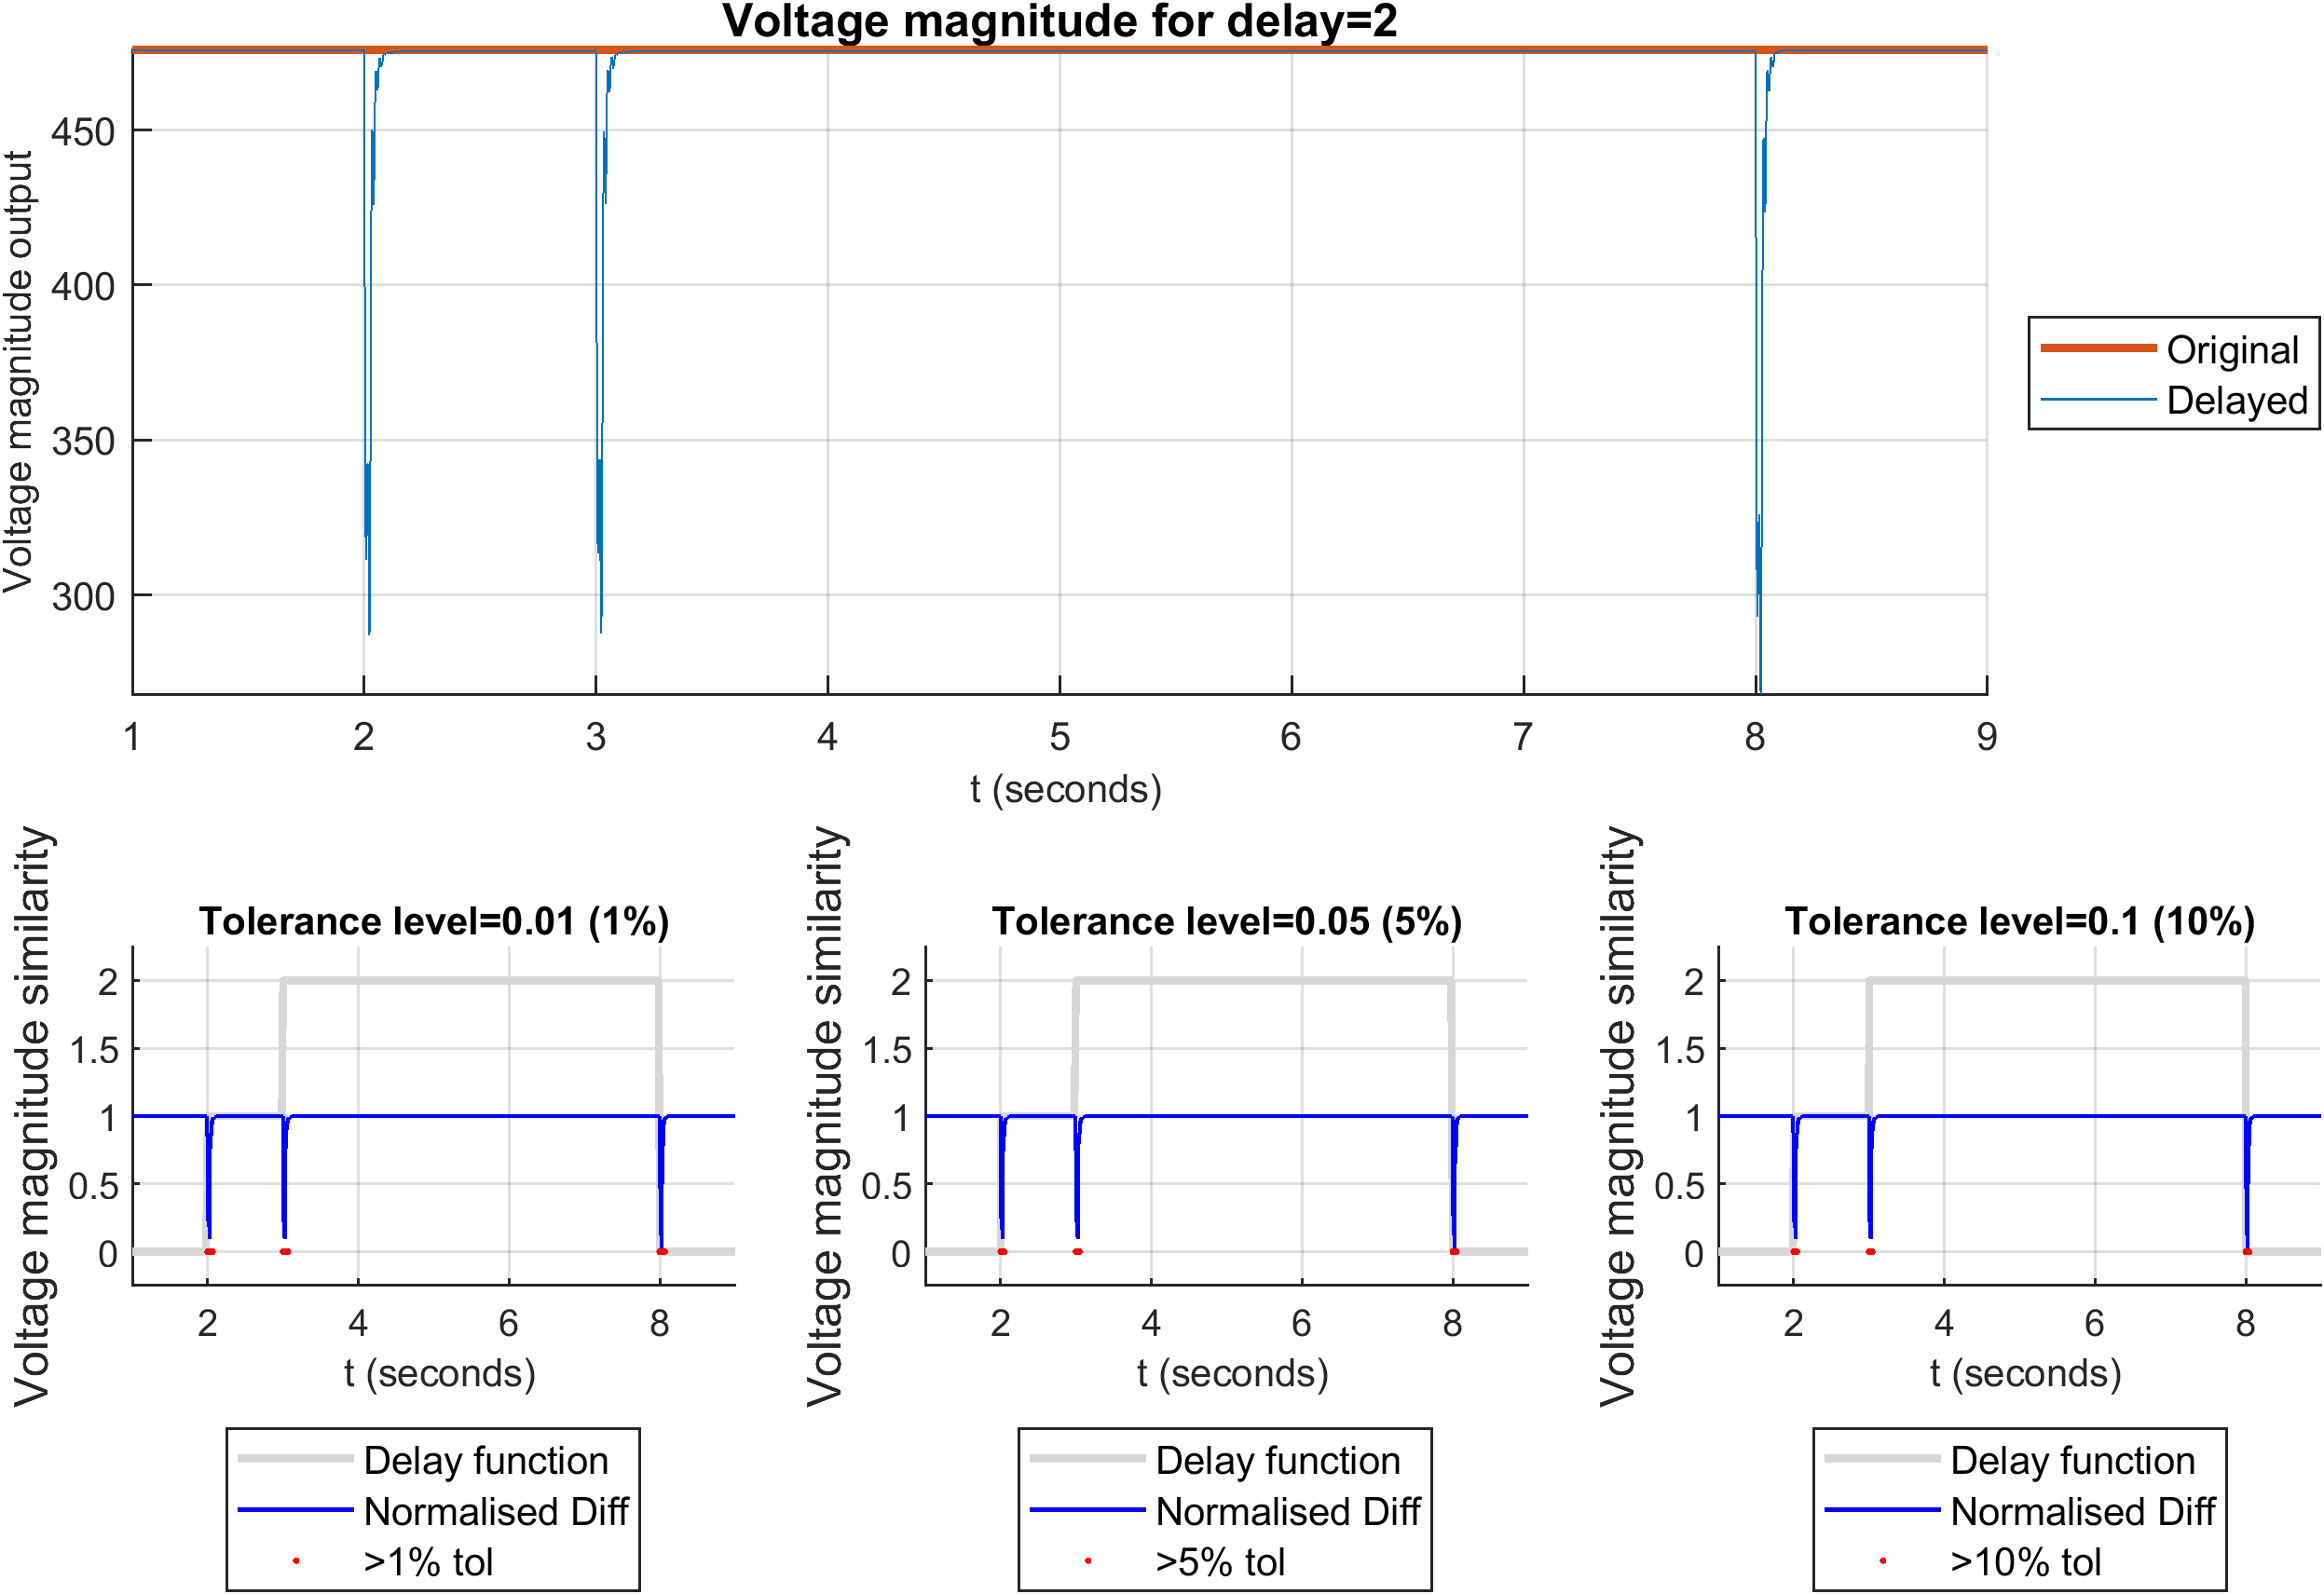
\includegraphics[width=0.95\textwidth]{PMUsim-figures/DelayOf_2/Step_vMagnitude.png}}\
  
    
   \fbox{  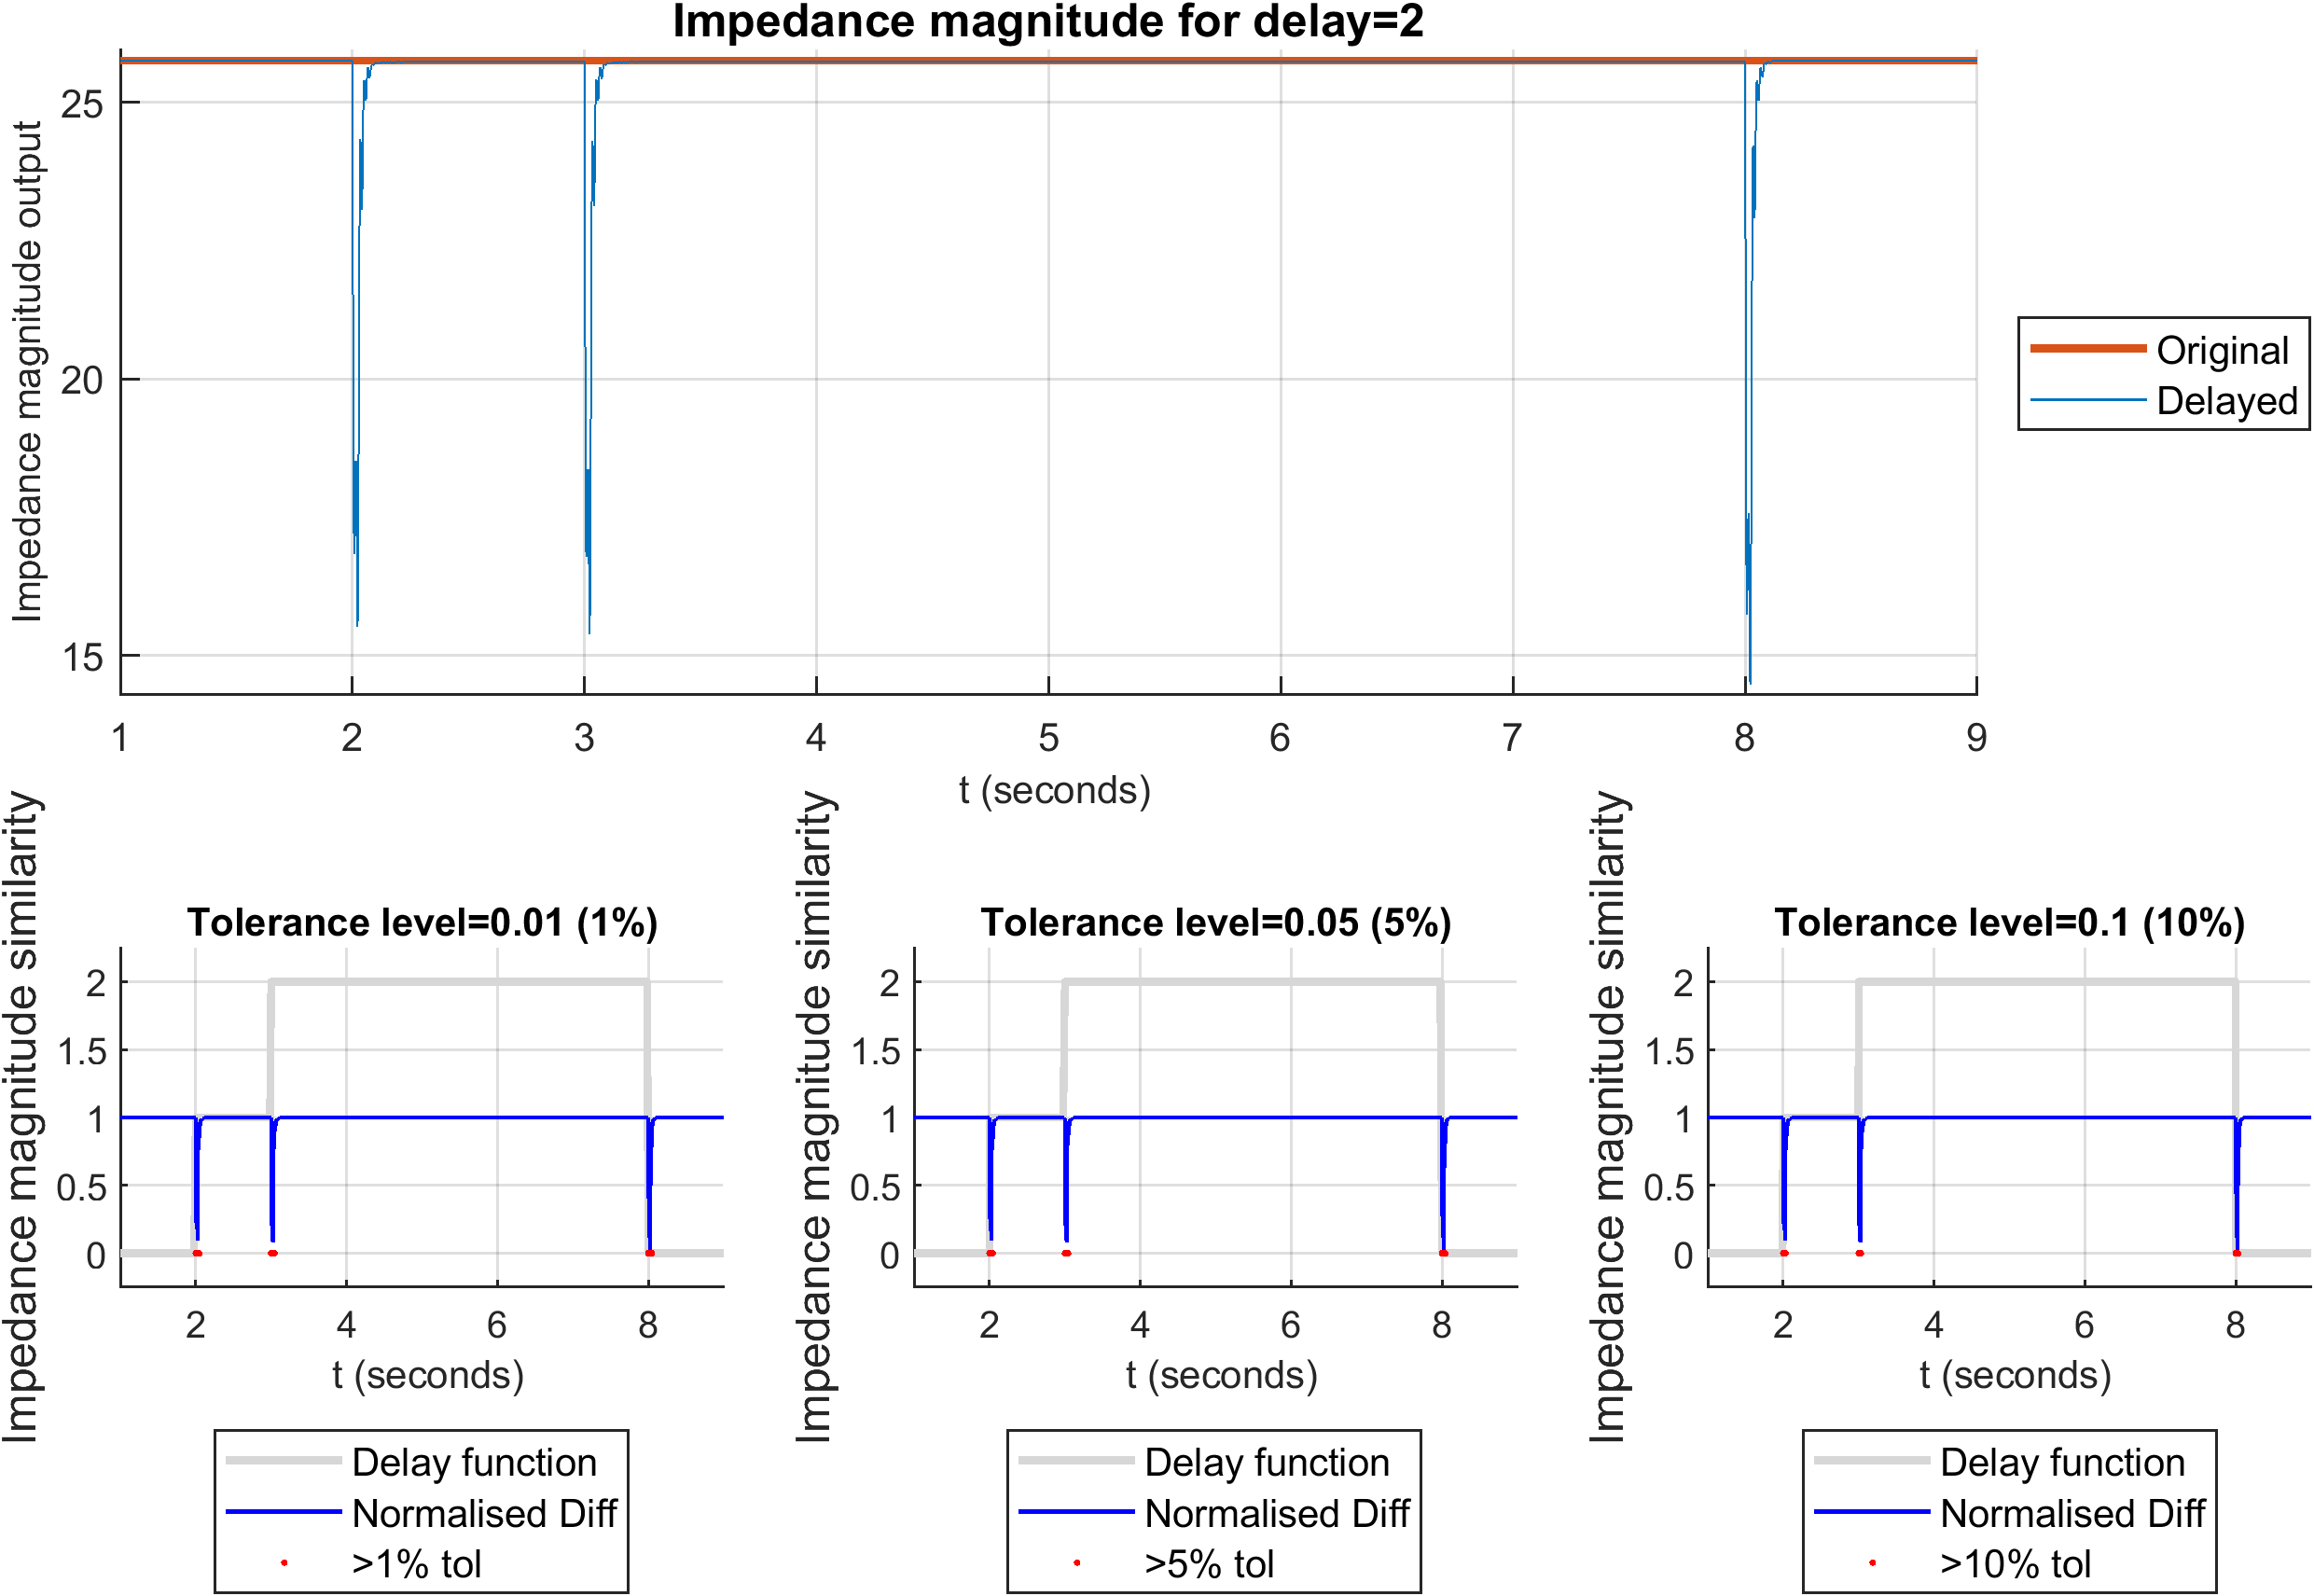
\includegraphics[width=0.95\textwidth]{PMUsim-figures/DelayOf_2/Step_iMagnitude.png}}\
 \label{fig:PMUsimStep_Two_Magnitude}
 %\caption{Step-Wise Delay Magnitude Output for the Delay Level of Two}
  \end{tabular}
 \end{table}
 
\newpage

\begin{table}[]
\caption{Results for Frequency Output}
   \fbox{    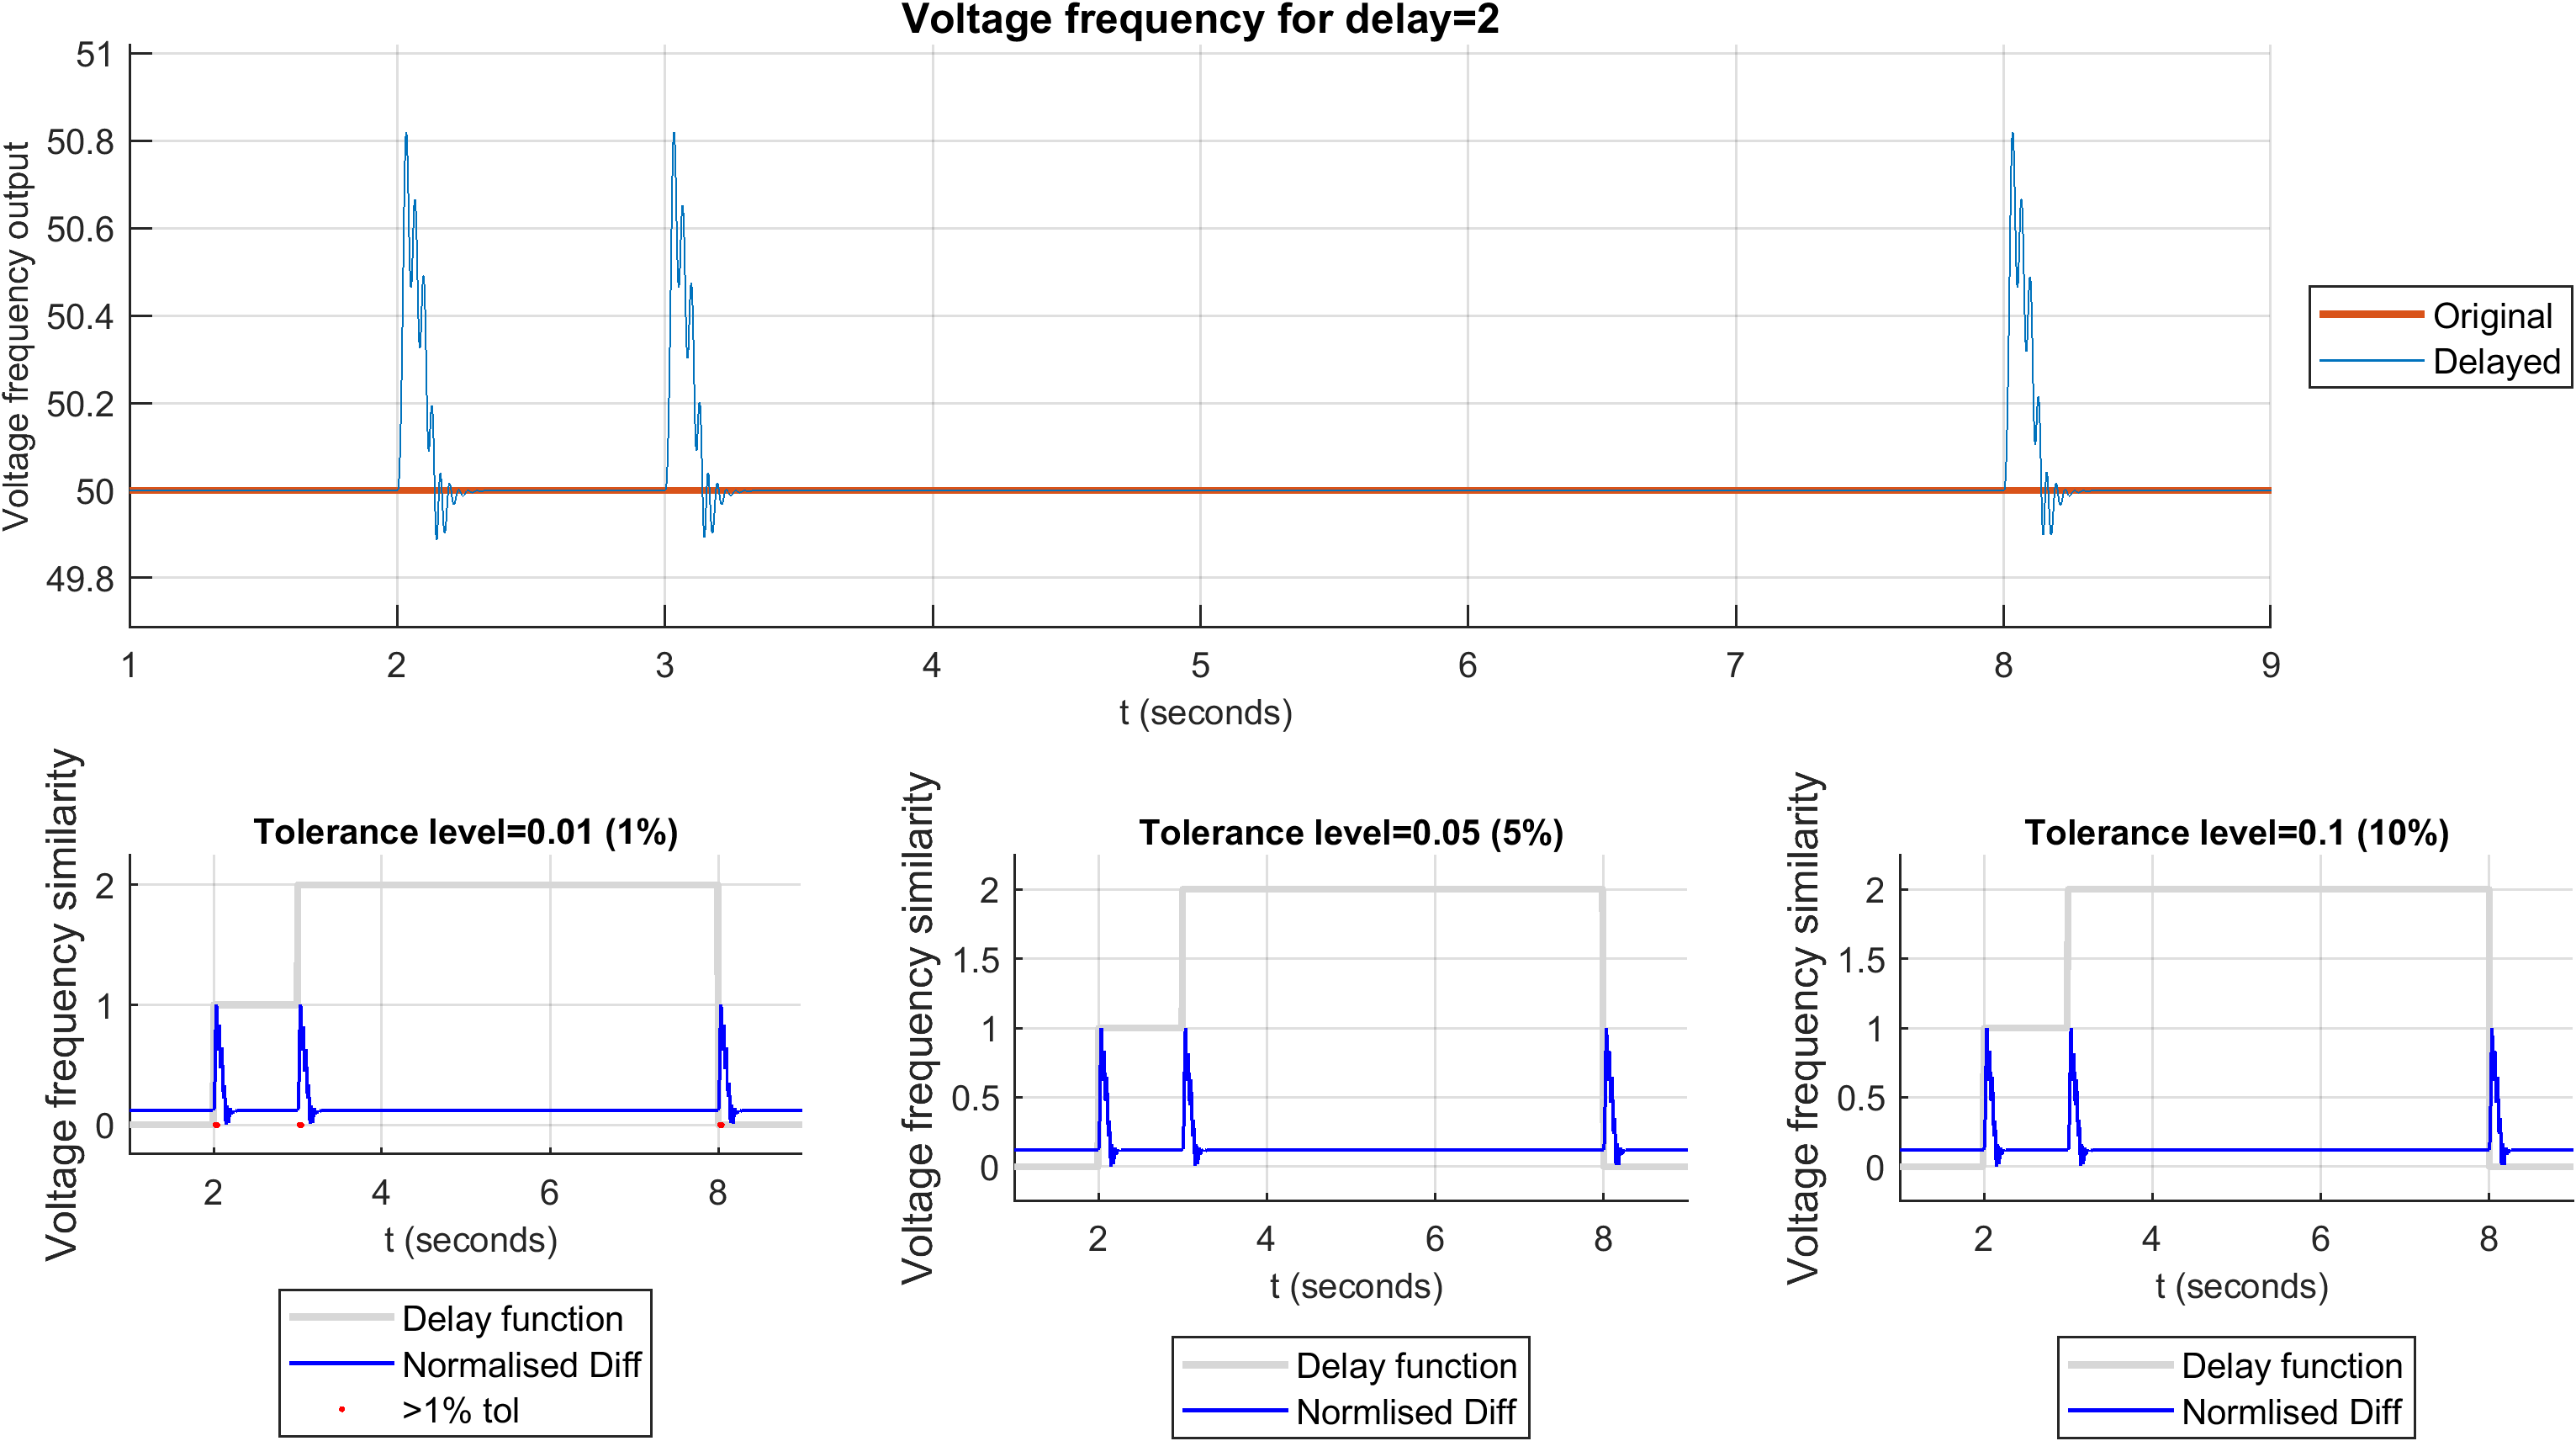
\includegraphics[width=0.95\textwidth]{PMUsim-figures/DelayOf_2/Step_vFrequency.png}}\
  
    
   \fbox{  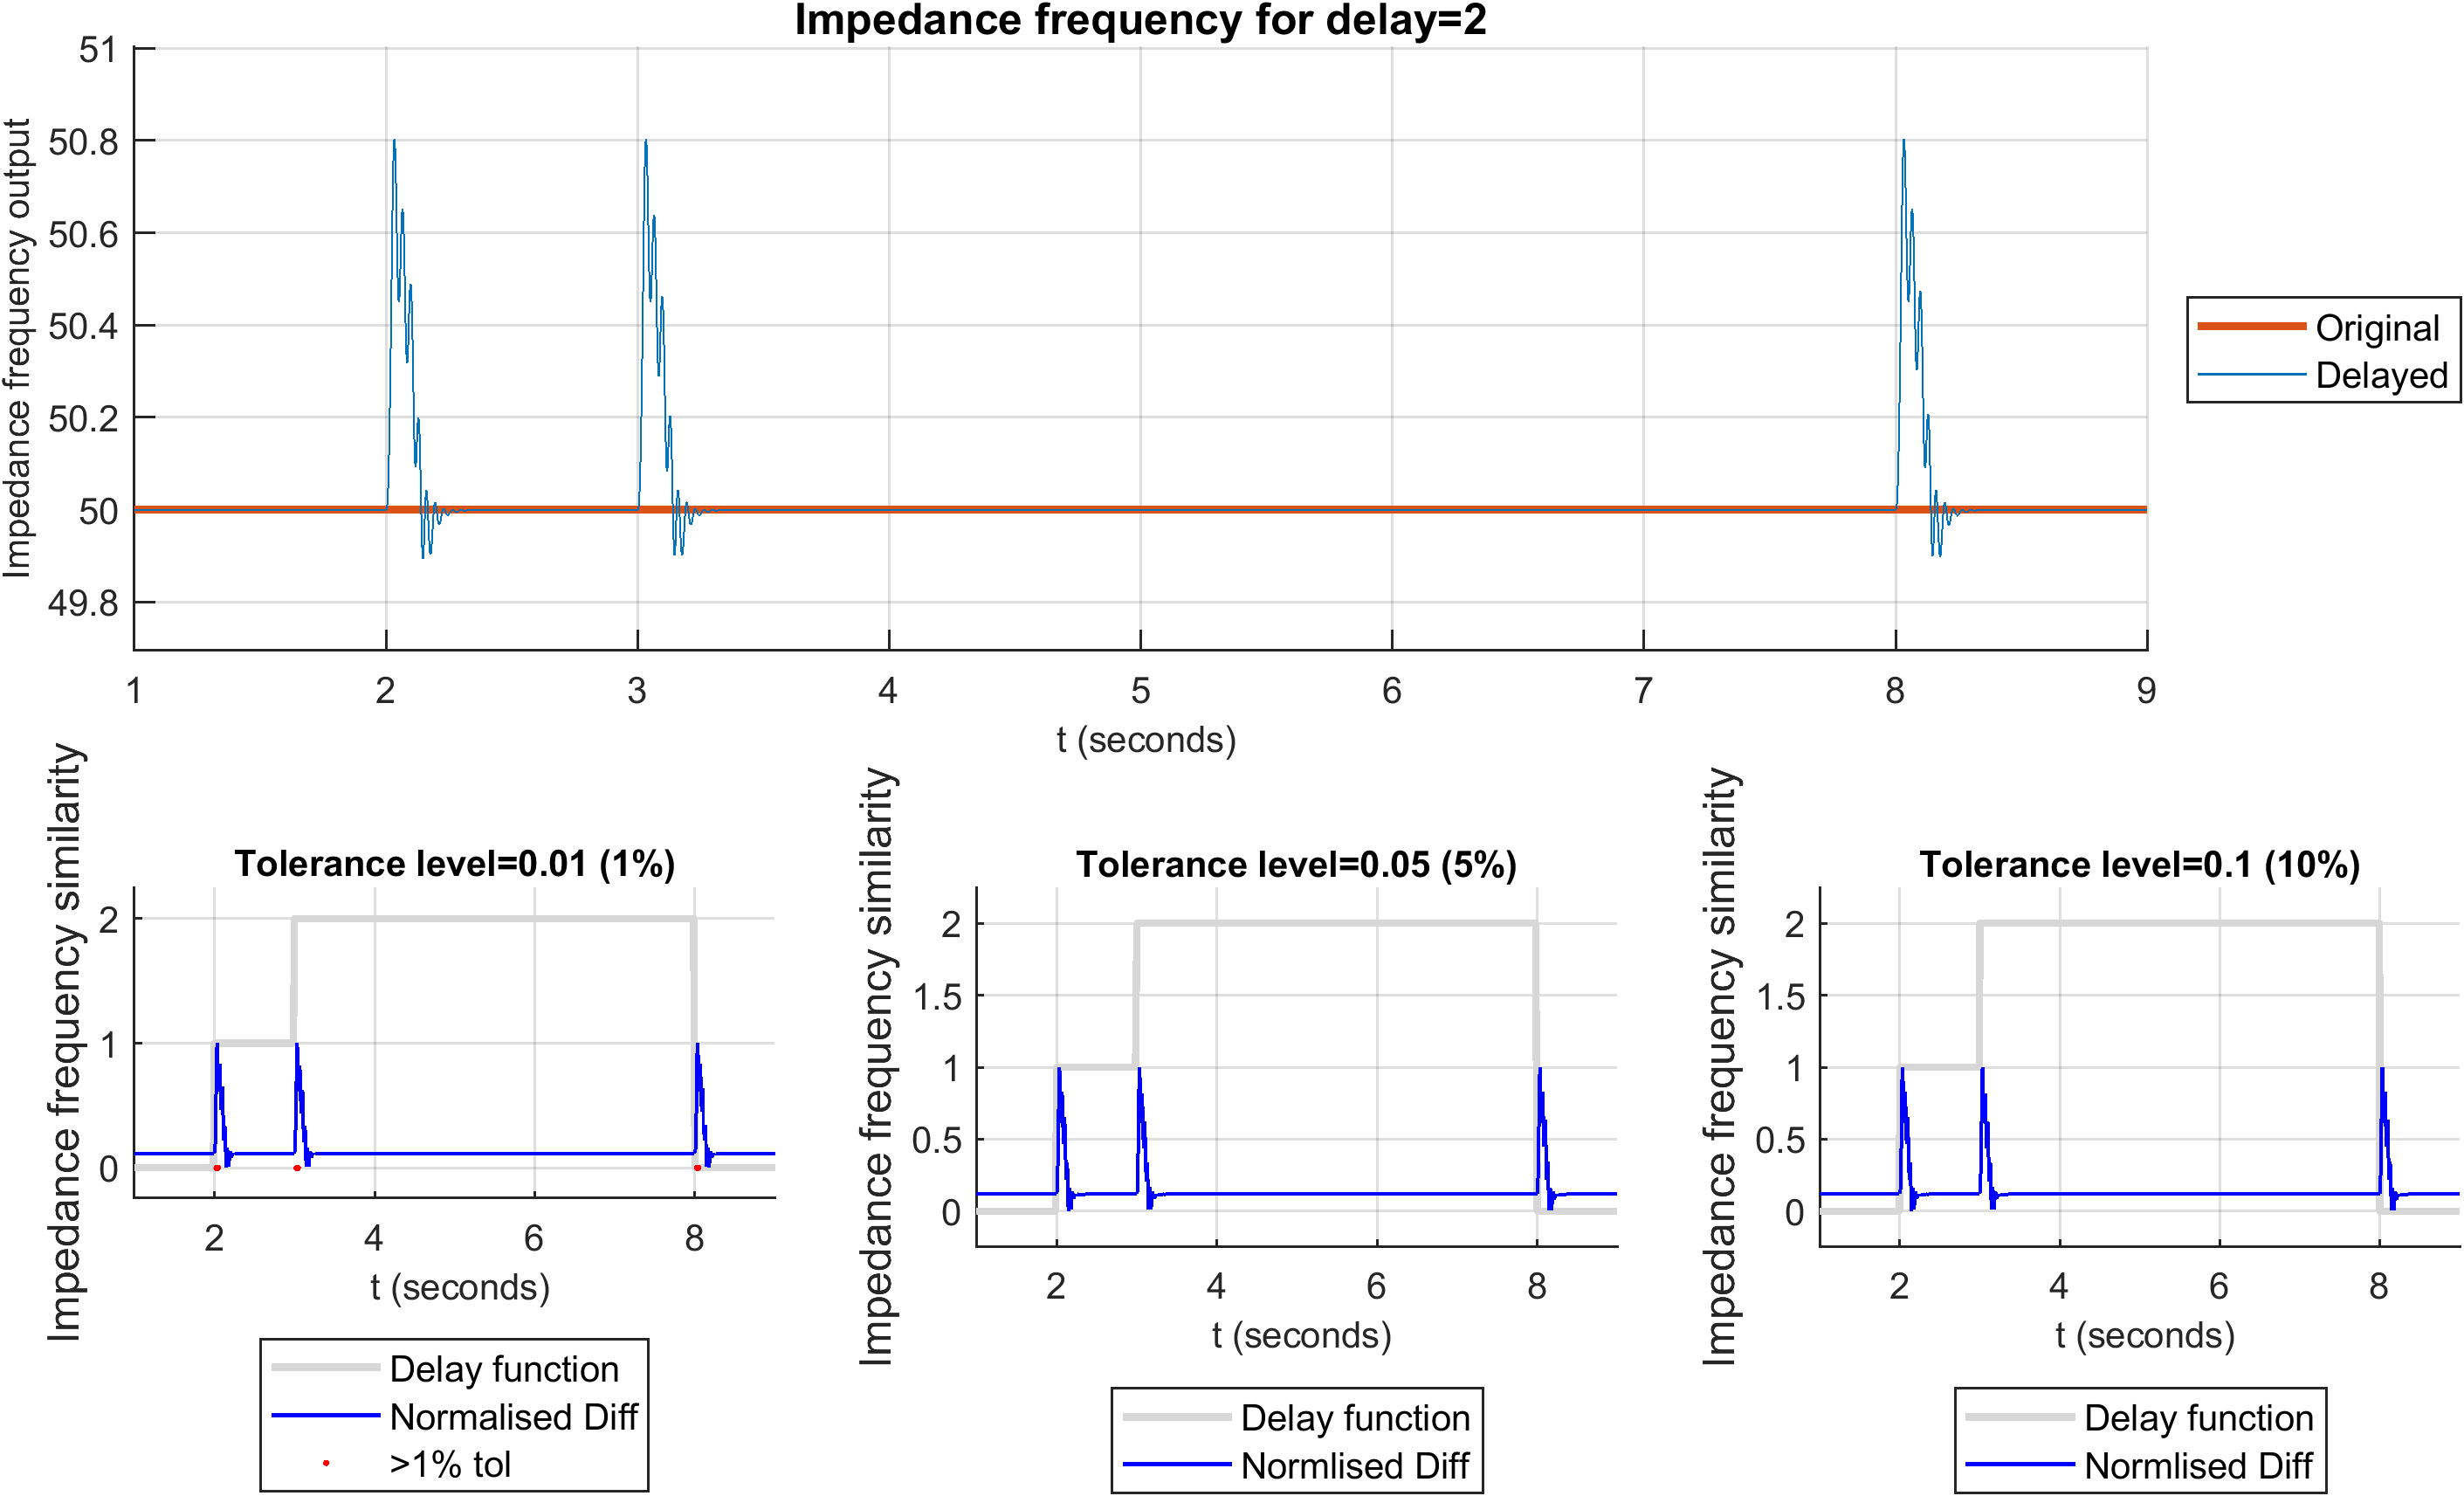
\includegraphics[width=0.95\textwidth]{PMUsim-figures/DelayOf_2/Step_iFrequency.png}}\
 \label{fig:PMUsimStep_Two_Frequency}
 %\caption{Step-Wise Delay Frequency Output for the Delay Level of Two}
  \end{tabular}
 \end{table}
 


\newpage

\begin{table}[]
\caption{Results for Angle Output}
   \fbox{     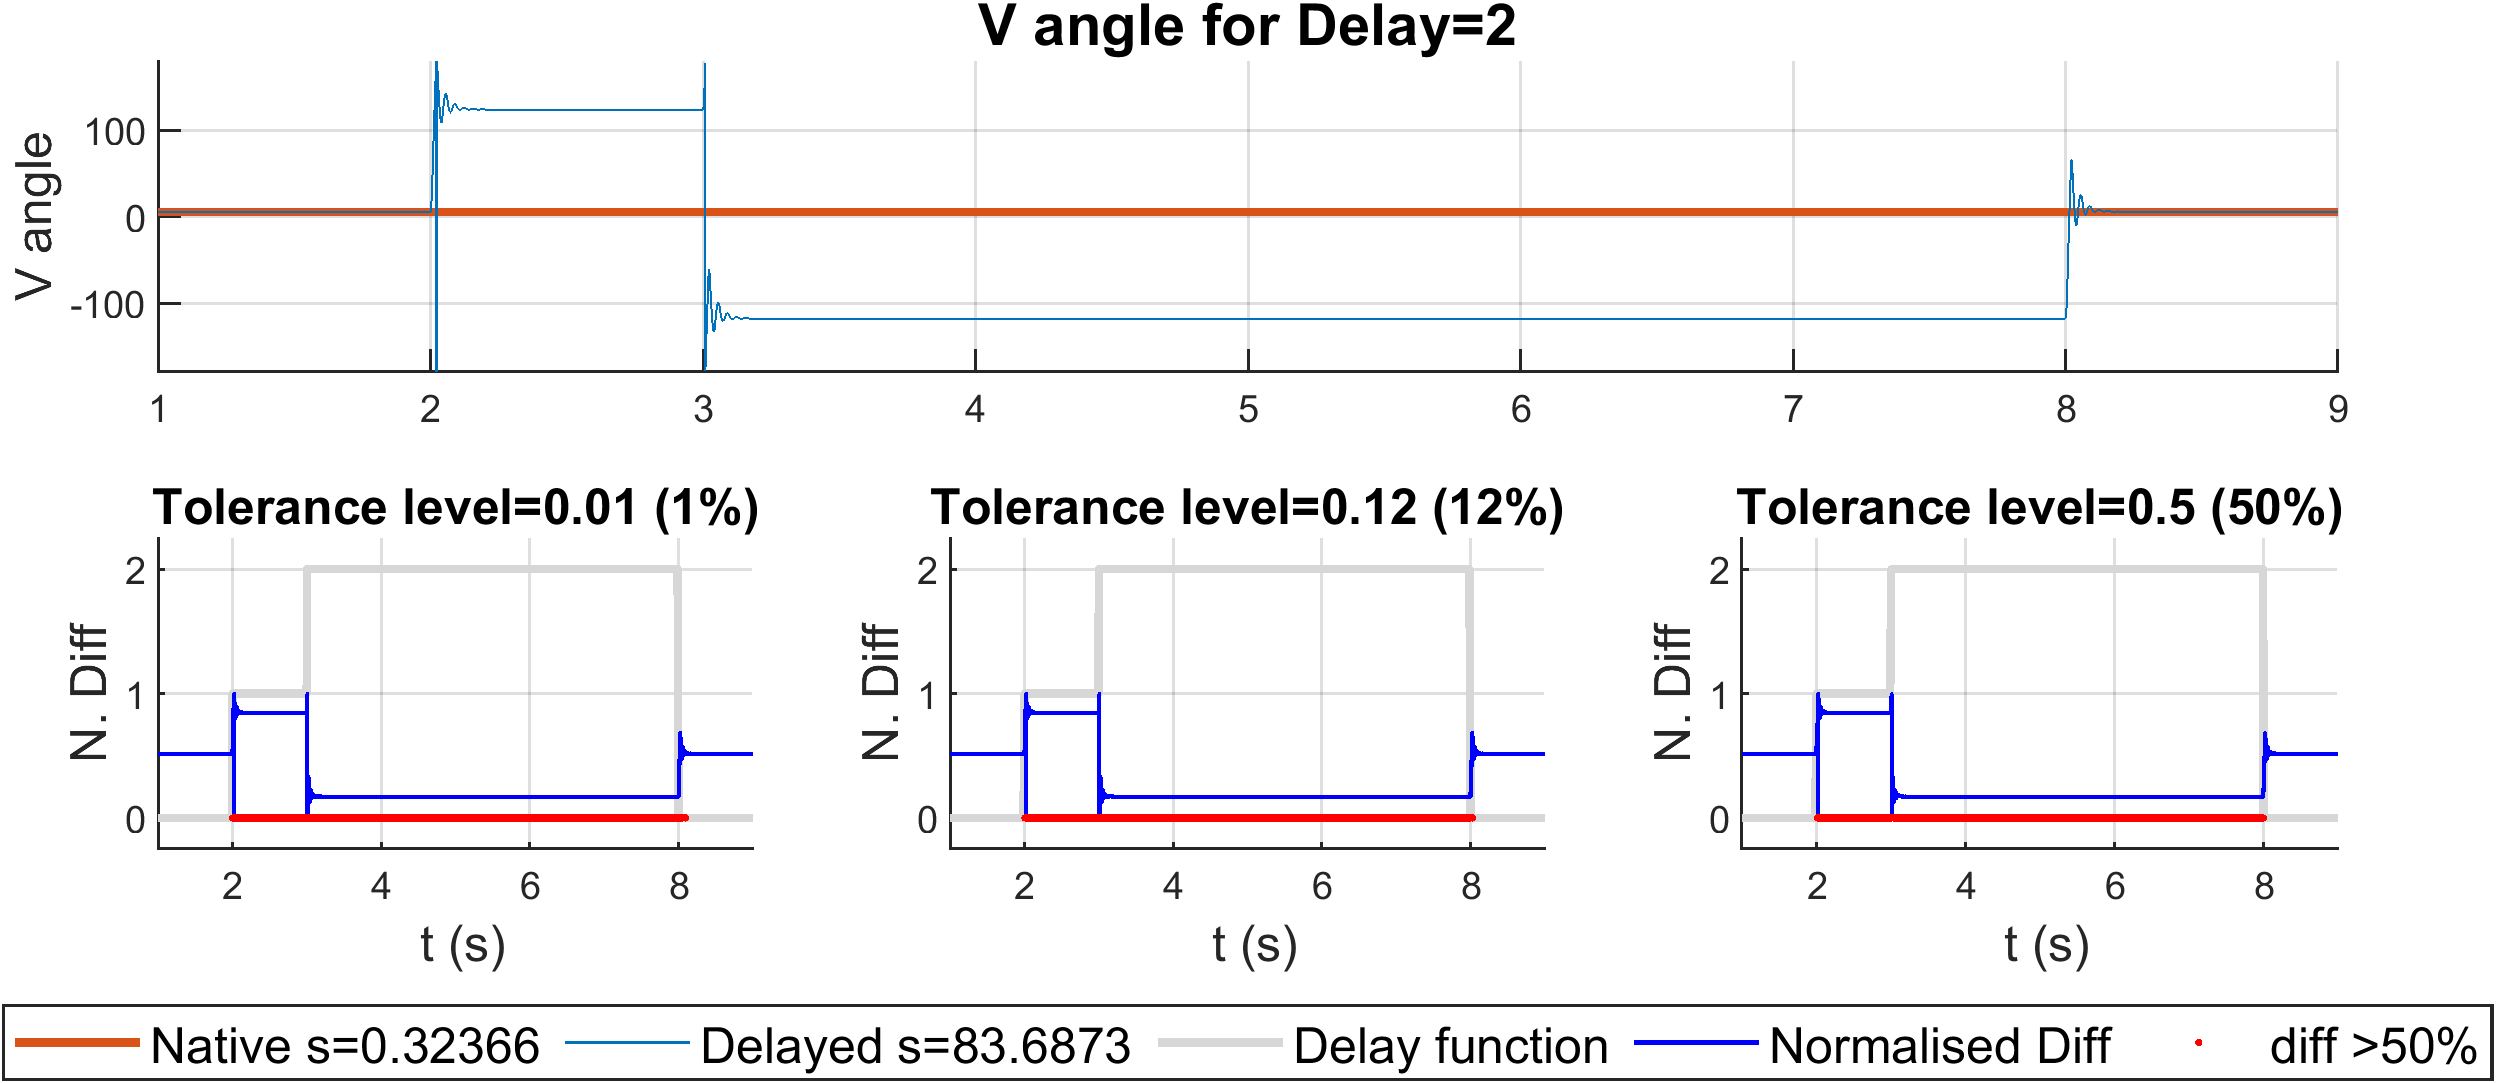
\includegraphics[width=0.95\textwidth]{PMUsim-figures/DelayOf_2/Step_vAngle.png}}\
  
    
   \fbox{ 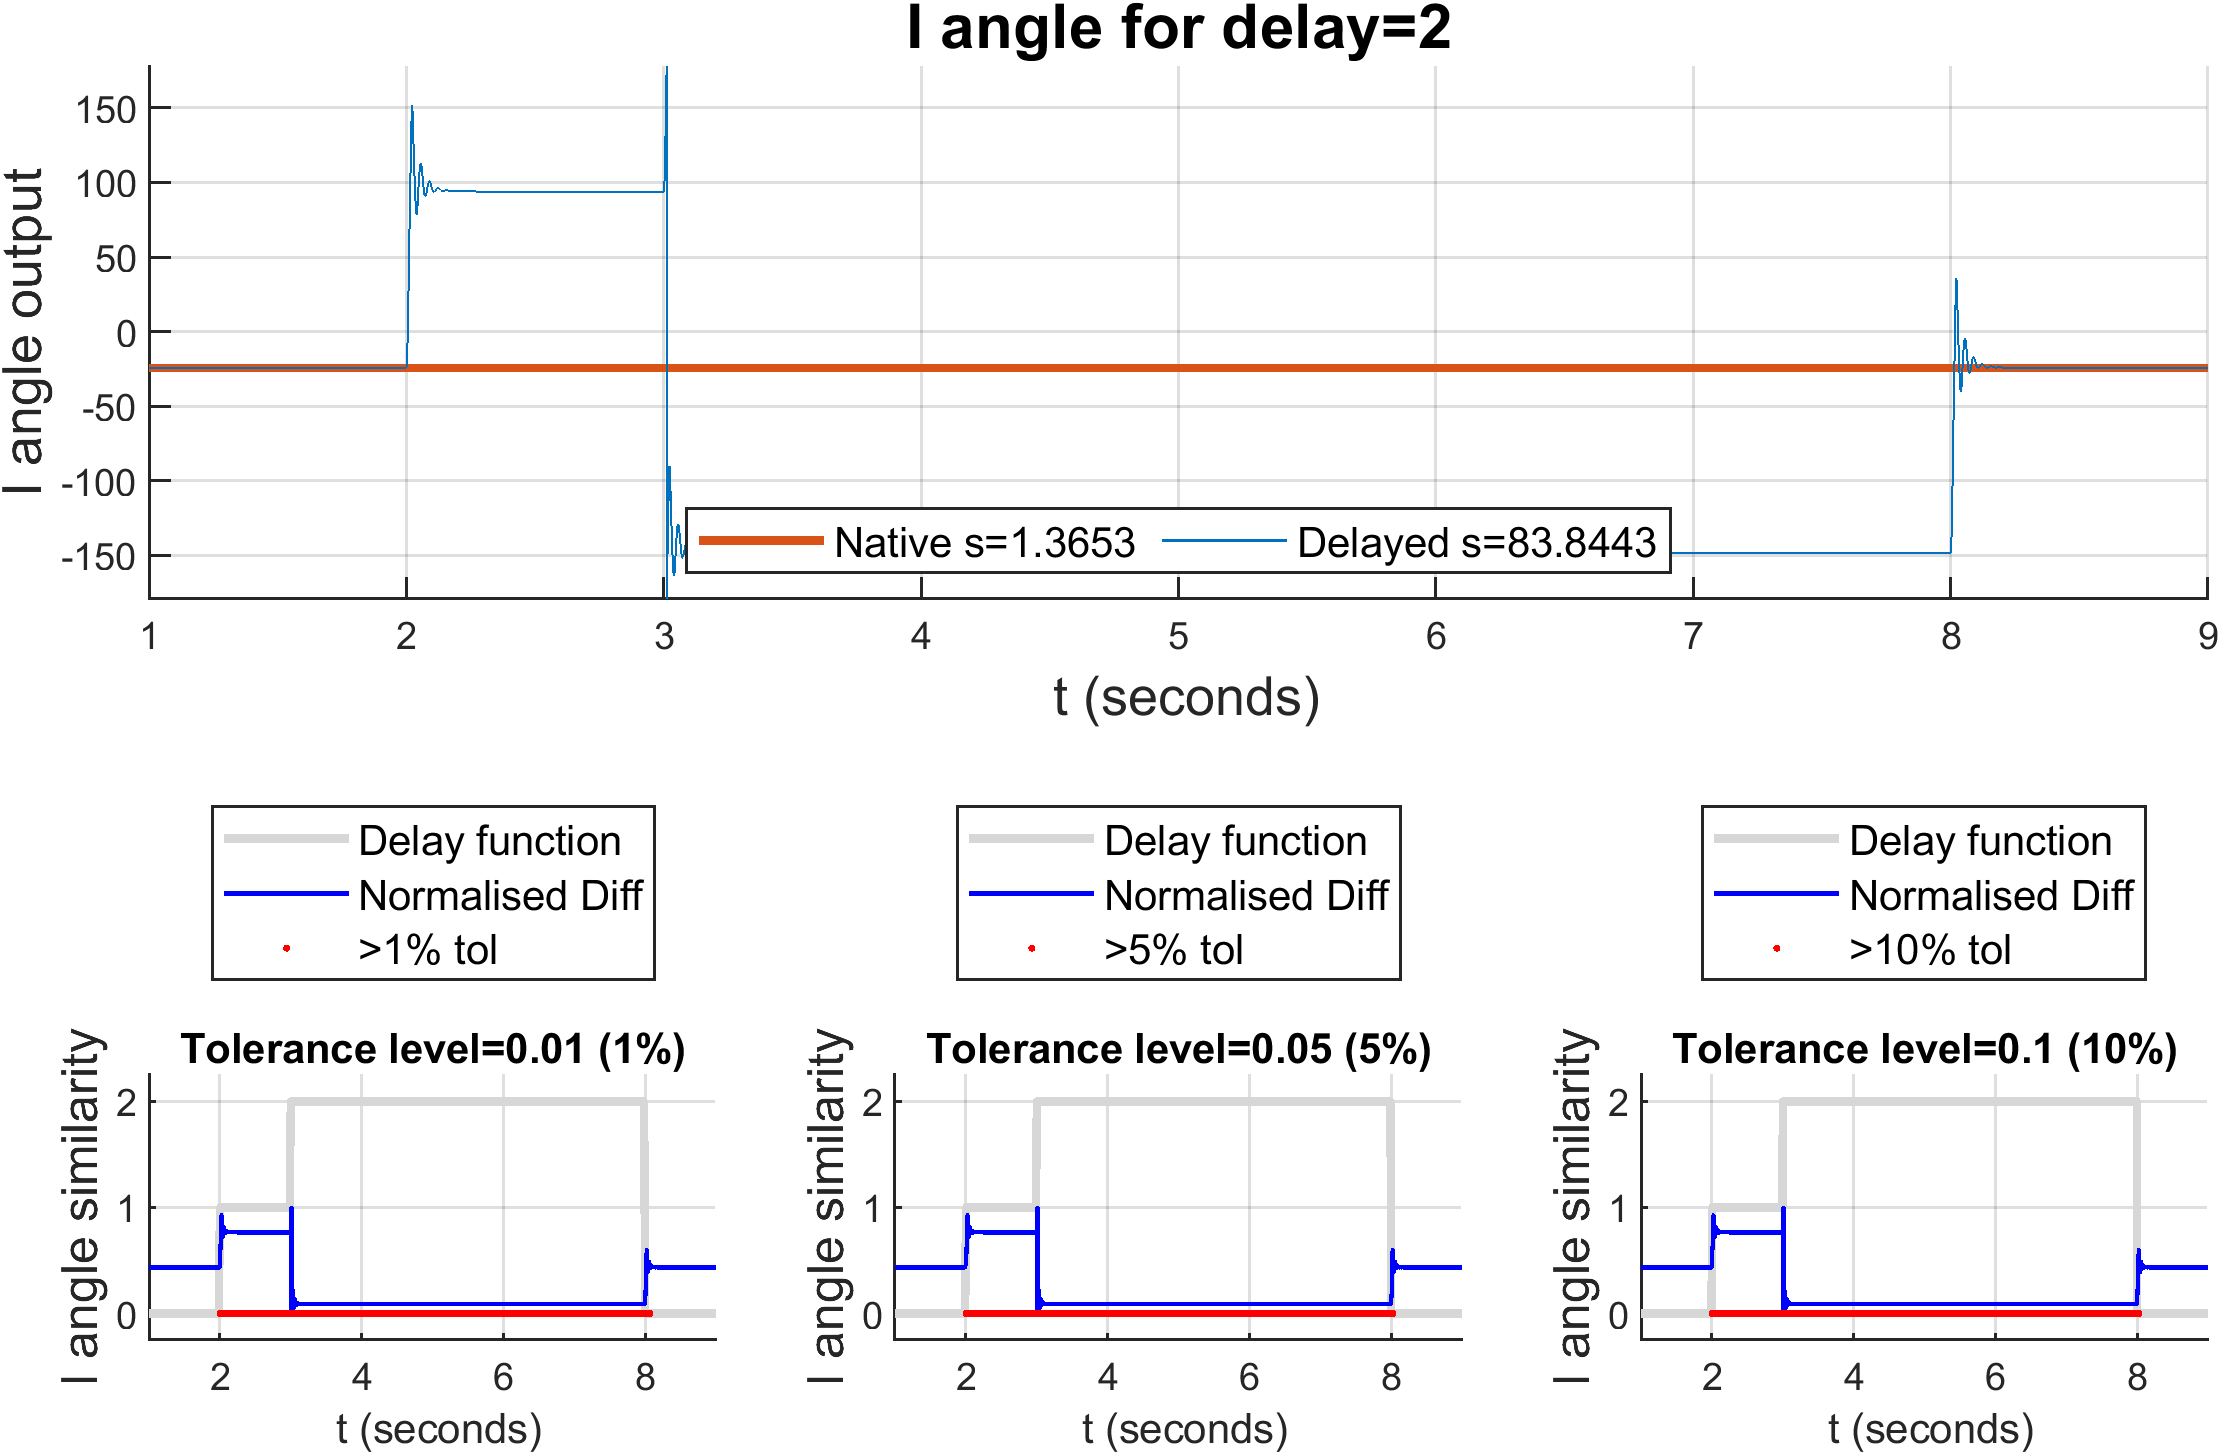
\includegraphics[width=0.95\textwidth]{PMUsim-figures/DelayOf_2/Step_iAngle.png}}\
 \label{fig:PMUsimStep_Two_Angle}
 %\caption{Step-Wise Delay Angle Output for the Delay Level of Two}
  \end{tabular}
 \end{table}


\newpage \subsection{Delay Level of Three}


\begin{table}[]
\caption{Results for Magnitude Output}
   \fbox{    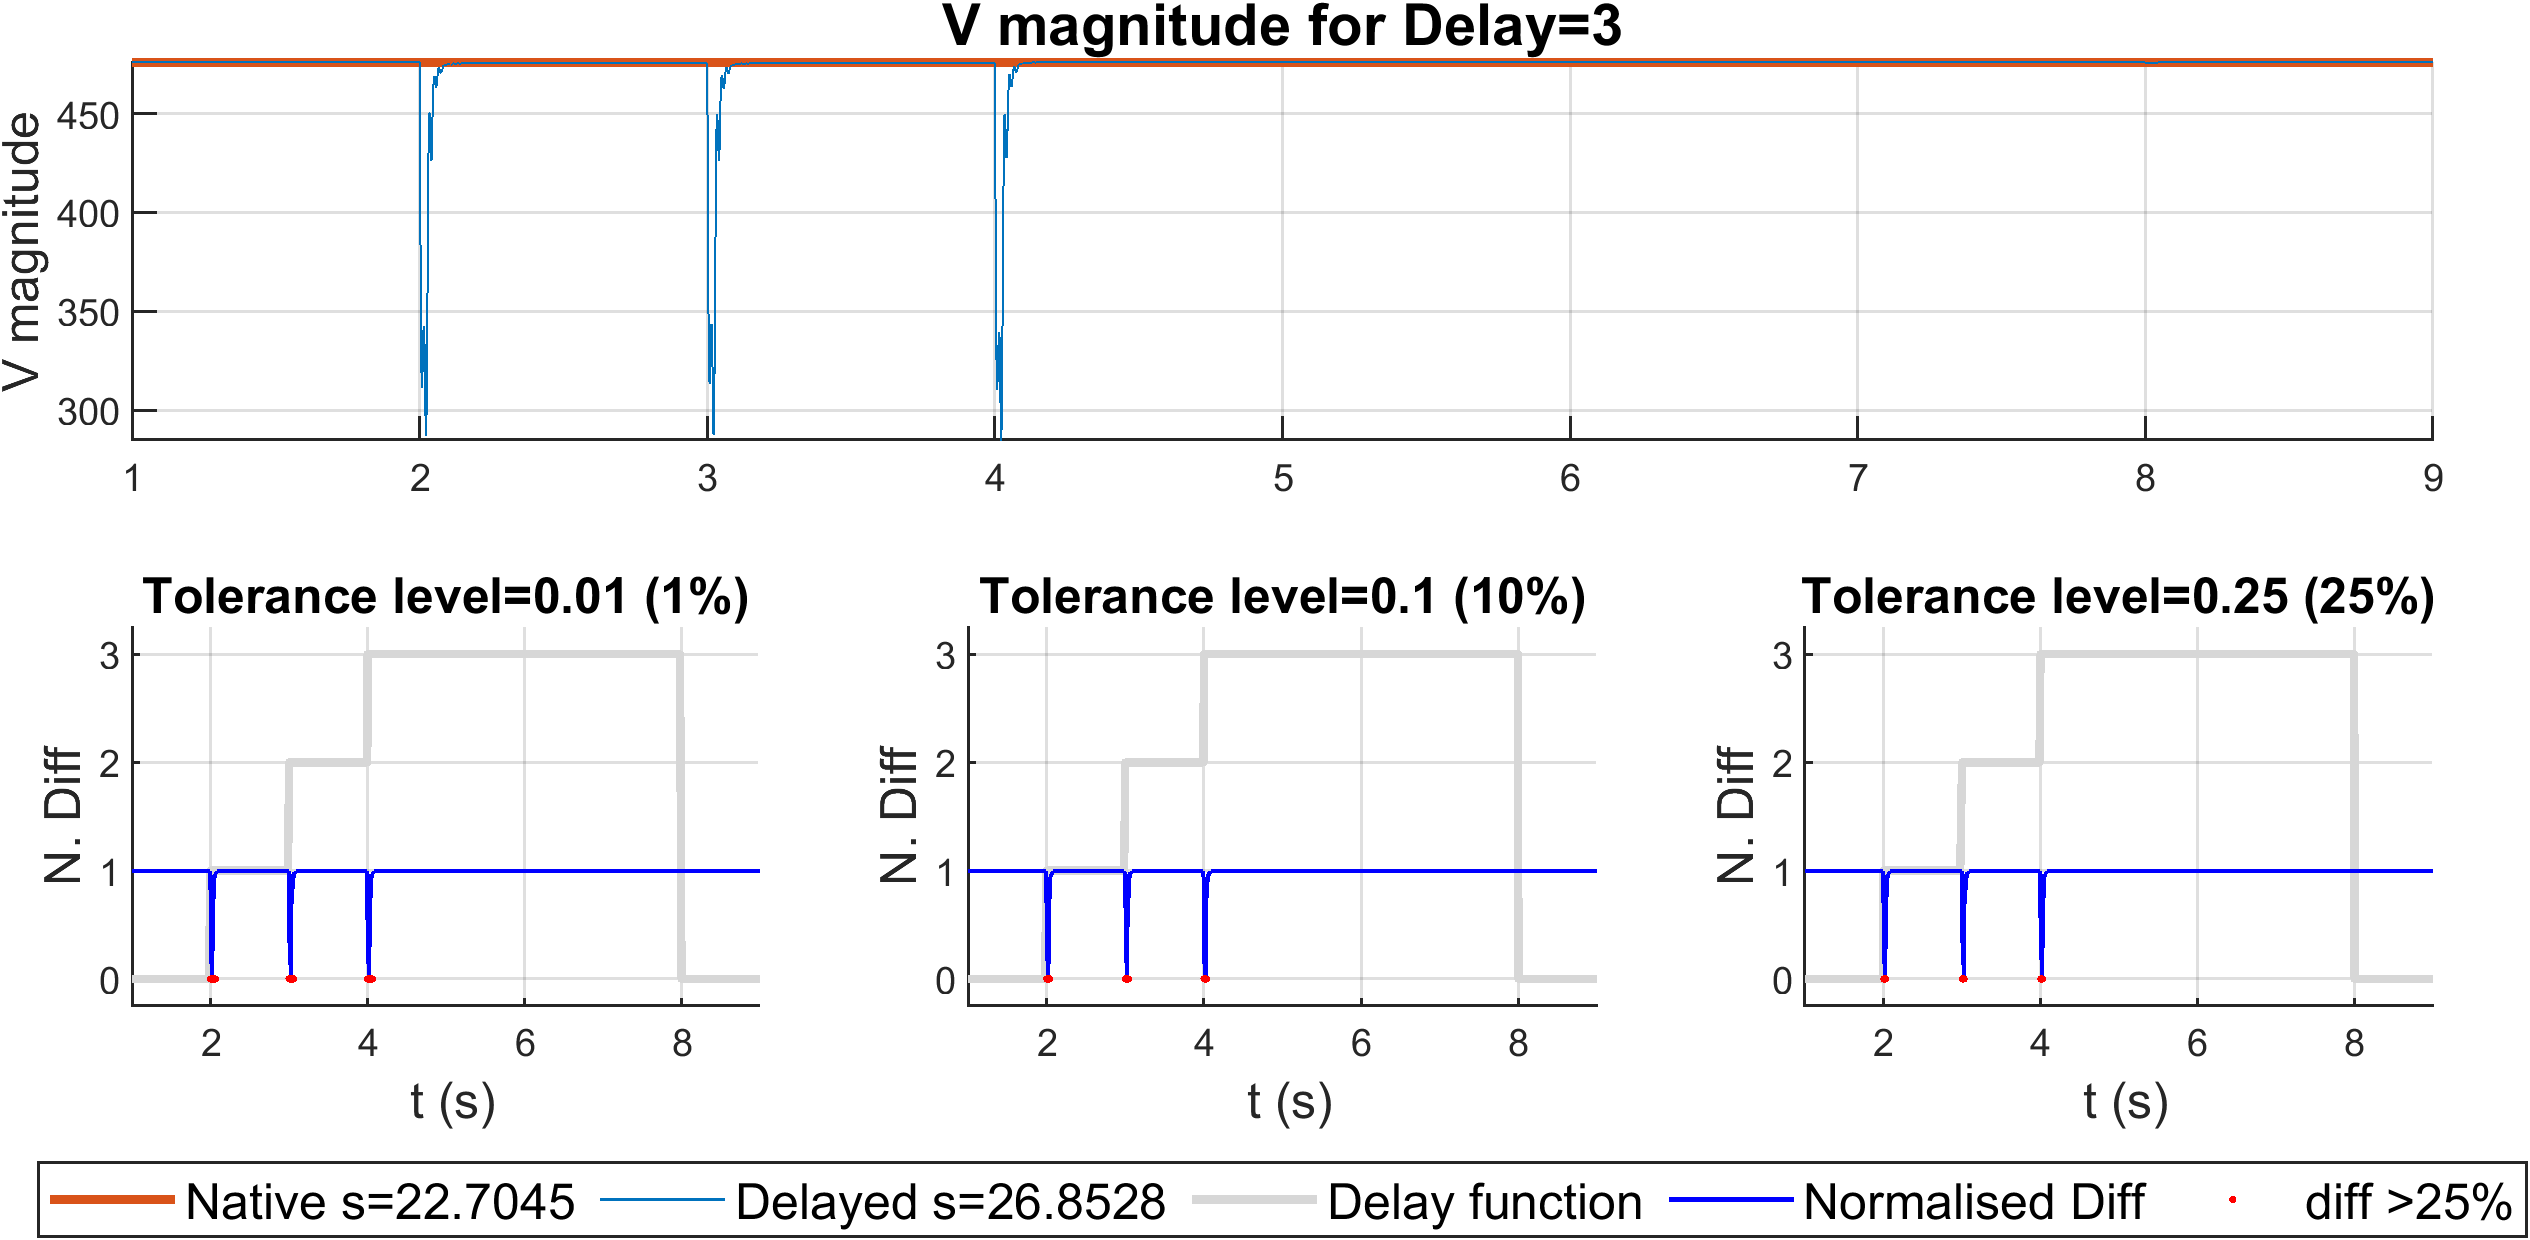
\includegraphics[width=0.95\textwidth]{PMUsim-figures/DelayOf_3/Step_vMagnitude.png}}\
  
    
   \fbox{  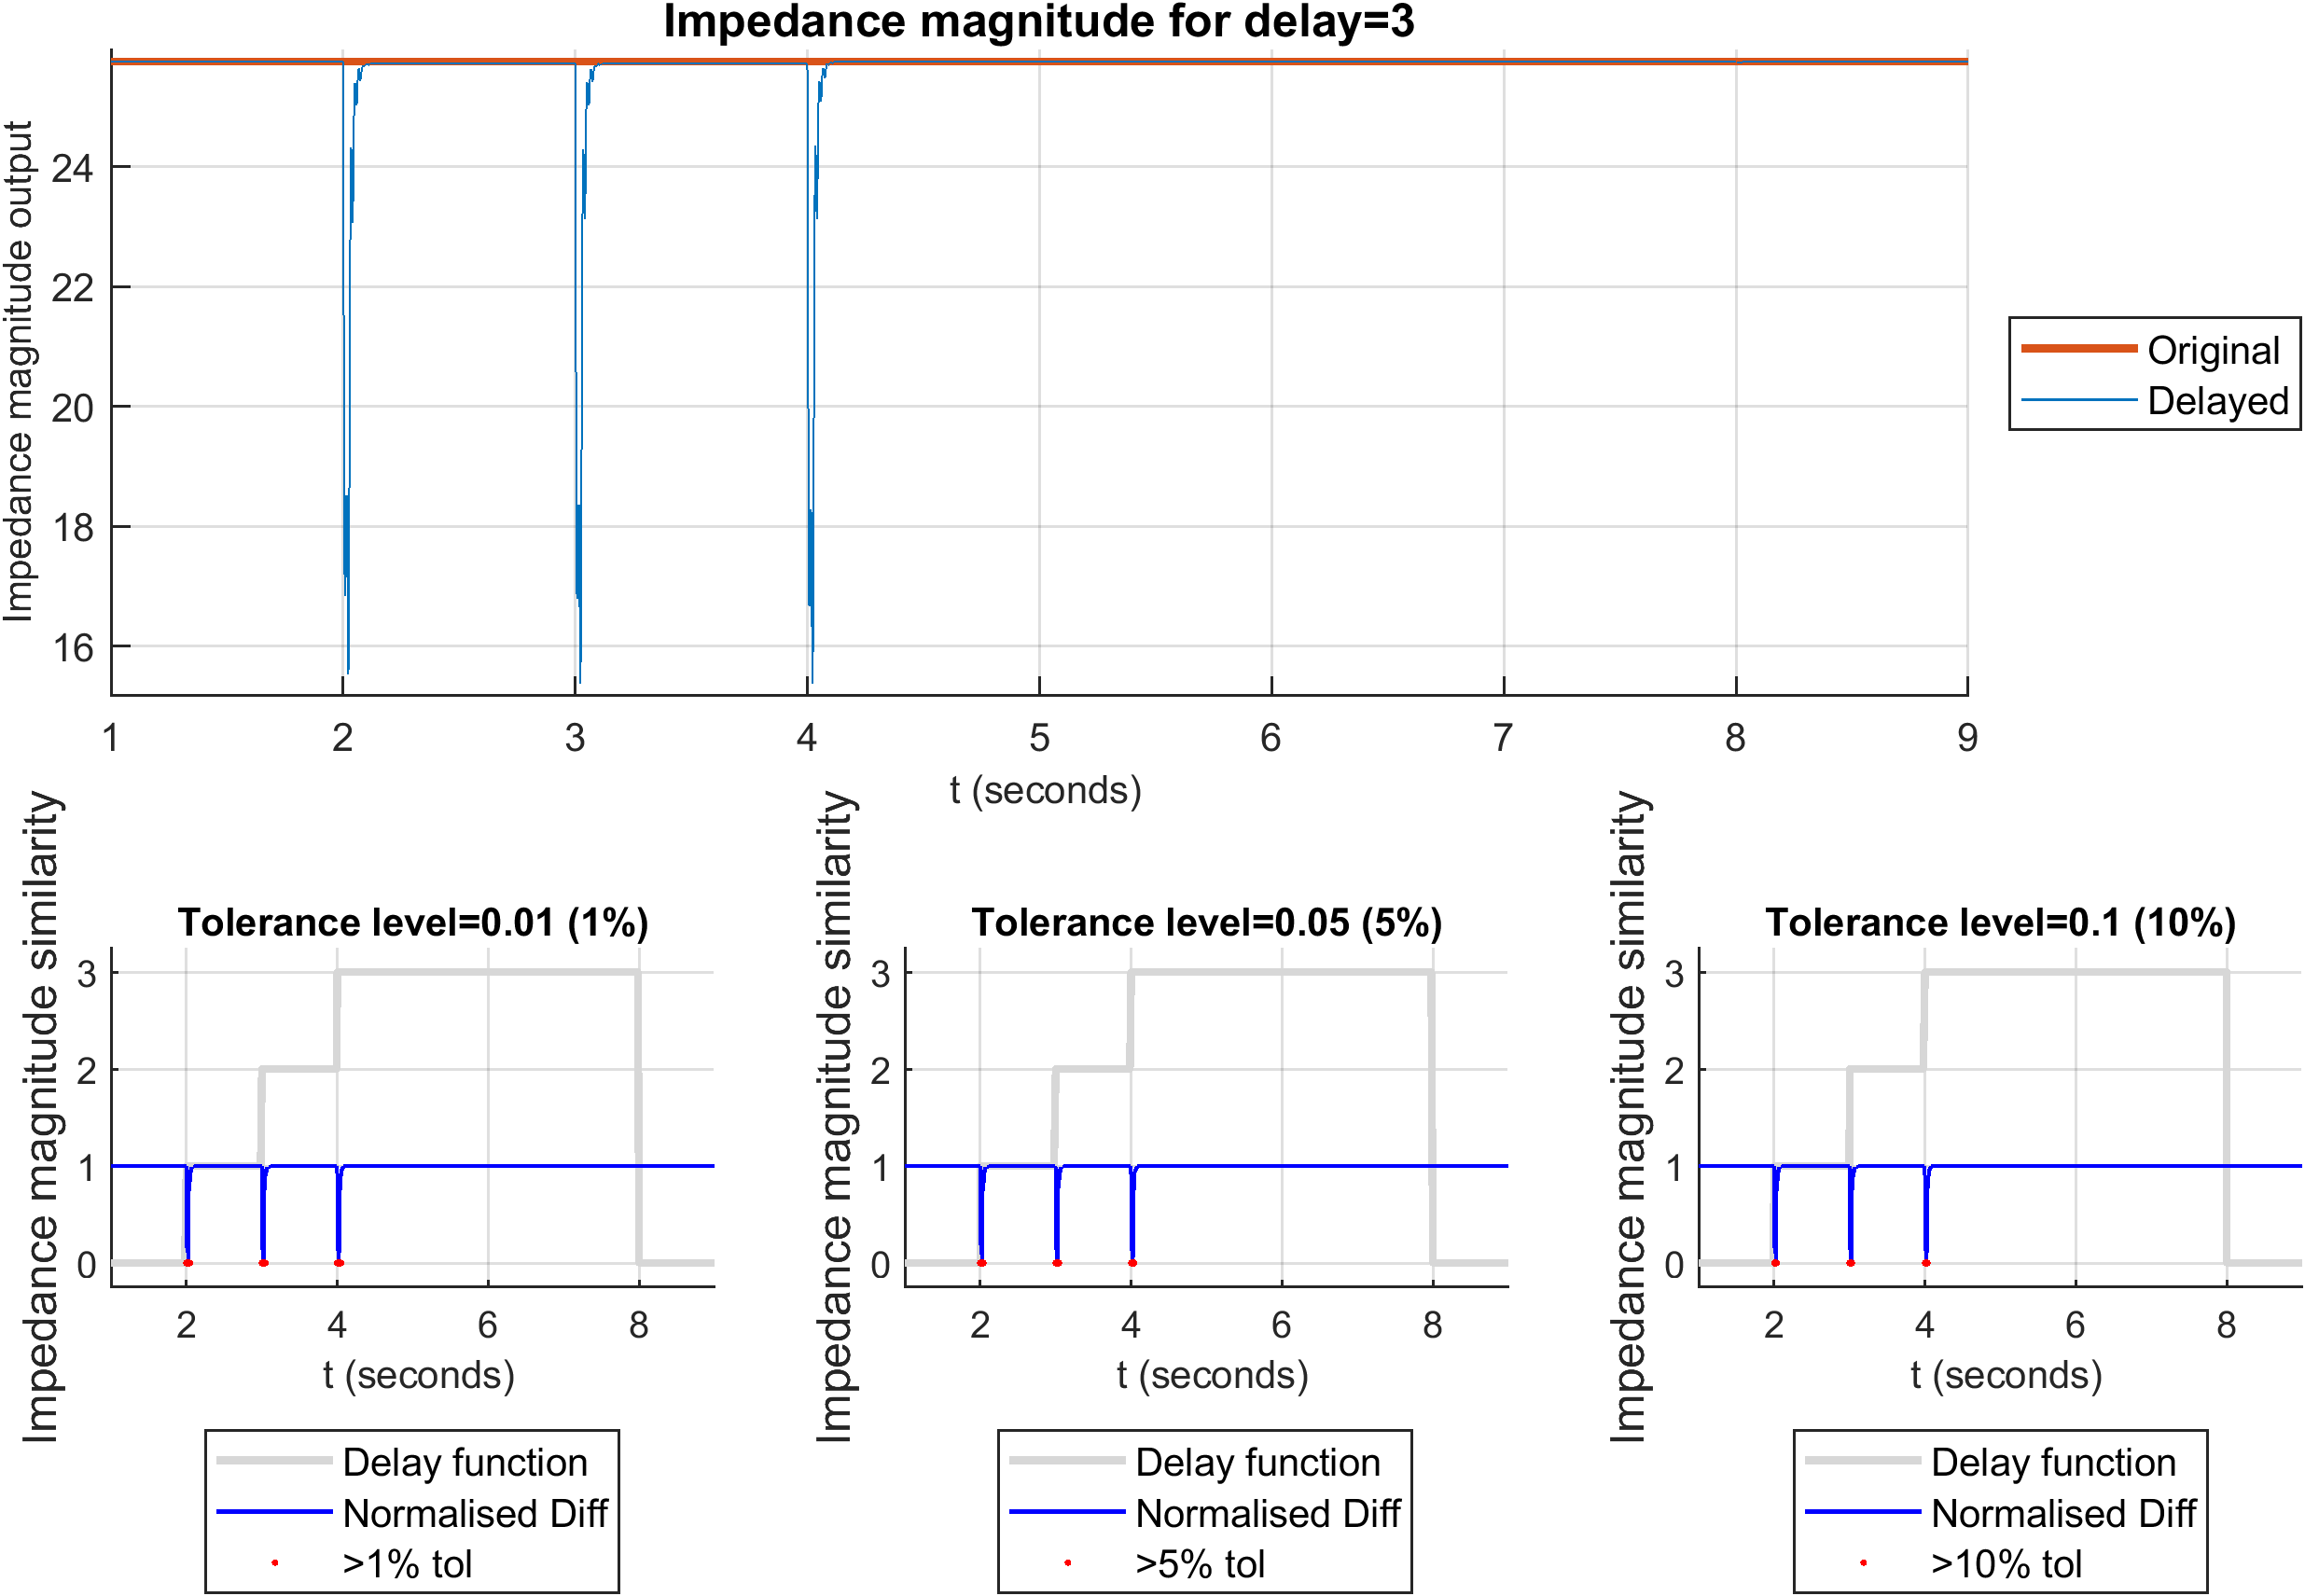
\includegraphics[width=0.95\textwidth]{PMUsim-figures/DelayOf_3/Step_iMagnitude.png}}\
 \label{fig:PMUsimStep_Three_Magnitude}
 %\caption{Step-Wise Delay Magnitude Output for the Delay Level of Three}
  \end{tabular}
 \end{table}



\newpage 

\begin{table}[]
\caption{Results for Frequency Output}
   \fbox{     \includegraphics[width=0.95\textwidth]{PMUsim-figures/DelayOf_3/Step_vFrequency.png}}\
  
    
   \fbox{  \includegraphics[width=0.95\textwidth]{PMUsim-figures/DelayOf_3/Step_iFrequency.png}}\
 \label{fig:PMUsimStep_Three_Frequency}
 %\caption{Step-Wise Delay Frequency Output for the Delay Level of Three}
  \end{tabular}
 \end{table}




\newpage 

\begin{table}[]
\caption{Results for Angle Output}
   \fbox{      \includegraphics[width=0.95\textwidth]{PMUsim-figures/DelayOf_3/Step_vAngle.png}}\
  
    
   \fbox{  \includegraphics[width=0.95\textwidth]{PMUsim-figures/DelayOf_3/Step_iAngle.png}}\
 \label{fig:PMUsimStep_Three_Angle}
 %\caption{Step-Wise Delay Angle Output for the Delay Level of Three}
  \end{tabular}
 \end{table}


\newpage \subsection{Delay Level of Four}


\begin{table}[]
\caption{Results for Magnitude Output}}{
     \begin{small}
         
     Comments:
        \begin{itemize}
            \item 
        \end{itemize}  
        \end{small}
   \fbox{    \includegraphics[width=0.95\textwidth]{PMUsim-figures/DelayOf_4/Step_vMagnitude.png}}\
  
    
   \fbox{   \includegraphics[width=0.95\textwidth]{PMUsim-figures/DelayOf_4/Step_iMagnitude.png}}\
 \label{fig:PMUsimStep_Four_Magnitude}
 %\caption{Step-Wise Delay Magnitude Output for the Delay Level of Four}
  \end{tabular}
 \end{table}



\newpage 

\begin{table}[]
\caption{Results for Frequency Output}
   \fbox{    \includegraphics[width=0.95\textwidth]{PMUsim-figures/DelayOf_4/Step_vFrequency.png}}\
  
    
   \fbox{  \includegraphics[width=0.95\textwidth]{PMUsim-figures/DelayOf_4/Step_iFrequency.png}}\
 \label{fig:PMUsimStep_Four_Frequency}
 %\caption{Step-Wise Delay Frequency Output for the Delay Level of Four}
  \end{tabular}
 \end{table}




\newpage 

\begin{table}[]
\caption{Results for Angle Output}
   \fbox{     \includegraphics[width=0.95\textwidth]{PMUsim-figures/DelayOf_4/Step_vAngle.png}}\
  
    
   \fbox{   \includegraphics[width=0.95\textwidth]{PMUsim-figures/DelayOf_4/Step_iAngle.png}}\
 \label{fig:PMUsimStep_Four_Angle}
 %\caption{Step-Wise Delay Angle Output for the Delay Level of Four}
  \end{tabular}
 \end{table}


\newpage \subsection{Delay Level of Five}


\begin{table}[]
\caption{Results for Magnitude Output}
   \fbox{     \includegraphics[width=0.95\textwidth]{PMUsim-figures/DelayOf_5/Step_vMagnitude.png}}\
  
    
   \fbox{   \includegraphics[width=0.95\textwidth]{PMUsim-figures/DelayOf_5/Step_iMagnitude.png}}\
 \label{fig:PMUsimStep_Five_Magnitude}
 %\caption{Step-Wise Delay Magnitude Output for the Delay Level of Five}
  \end{tabular}
 \end{table}


\newpage 

\begin{table}[]
\caption{Results for Frequency Output}
   \fbox{     \includegraphics[width=0.95\textwidth]{PMUsim-figures/DelayOf_5/Step_vFrequency.png}}\
  
    
   \fbox{  \includegraphics[width=0.95\textwidth]{PMUsim-figures/DelayOf_5/Step_iFrequency.png}}\
 \label{fig:PMUsimStep_Five_Frequency}
 %\caption{Step-Wise Delay Frequency Output for the Delay Level of Five}
  \end{tabular}
 \end{table}


\newpage 

\begin{table}[]
\caption{Results for Angle Output} 
   \fbox{    \includegraphics[width=0.95\textwidth]{PMUsim-figures/DelayOf_5/Step_vAngle.png}}\
  
    
   \fbox{   \includegraphics[width=0.95\textwidth]{PMUsim-figures/DelayOf_5/Step_iAngle.png}}\  
 \label{fig:PMUsimStep_Five_Angle}
 %\caption{Step-Wise Delay Angle Output for the Delay Level of Five}
  \end{tabular}
 \end{table}



\newpage \subsection{Delay Level of Six} 




\begin{table}[]
\caption{Results for Magnitude Output} 
   \fbox{     \includegraphics[width=0.95\textwidth]{PMUsim-figures/DelayOf_6/Step_vMagnitude.png}}\
  
    
   \fbox{   \includegraphics[width=0.95\textwidth]{PMUsim-figures/DelayOf_6/Step_iMagnitude.png}}\
 \label{fig:PMUsimStep_Six_Magnitude}
 %\caption{Step-Wise Delay Magnitude Output for the Delay Level of Six}
  \end{tabular}
 \end{table}



\newpage 

\begin{table}[]
\caption{Results for Frequency Output} 
   \fbox{    \includegraphics[width=0.95\textwidth]{PMUsim-figures/DelayOf_6/Step_vFrequency.png}}\
  
    
   \fbox{   \includegraphics[width=0.95\textwidth]{PMUsim-figures/DelayOf_6/Step_iFrequency.png}}\
 \label{fig:PMUsimStep_Six_Frequency}
 %\caption{Step-Wise Delay Frequency Output for the Delay Level of Six}
  \end{tabular}
 \end{table}

 
\newpage 

 


\begin{table}[]
\caption{Results for Angle Output}
   \fbox{     \includegraphics[width=0.95\textwidth]{PMUsim-figures/DelayOf_6/Step_vAngle.png}}\
  
    
   \fbox{  \includegraphics[width=0.95\textwidth]{PMUsim-figures/DelayOf_6/Step_iAngle.png}}\
 \label{fig:PMUsimStep_Six_Angle}
 %\caption{Step-Wise Delay Angle Output for the Delay Level of Six}
  \end{tabular}
 \end{table}

\newpage





\newpage
\section{The Delay Level of Zero}
For model verification purposes, the output for the delay level of zero is included.

\begin{small}
     \tcbox[size=normal, standard jigsaw, opacityback=0, boxrule=0pt,halign=justify]{
     Comment on the figure:}{
          \begin{itemize}
         \item      The delayed signal (blue) overlaps the original signal (red), producing a straight line, colored neither red nor blue.
         \item  The blue Normalised diff signal also overlaps the grey delay function.
          \end{itemize} }
\end{small}



\newpage
\begin{figure}[H]
\begin{tabular}{c}
  \fbox{  \includegraphics[width=0.95\textwidth]{PMUsim-figures/DelayOf_0/Zero_vMagnitude.png}} \\ 
   
   \fbox{    \includegraphics[width=0.95\textwidth]{PMUsim-figures/DelayOf_0/Zero_vFrequency.png}} \\ 

   \fbox{     \includegraphics[width=0.95\textwidth]{PMUsim-figures/DelayOf_0/Zero_vAngle.png}}

  \end{tabular}
\label{fig:VoltageZeroDelay}
\caption{Results for Voltage Output for Delay equal to Zero }
\end{figure}



\newpage
\begin{figure}[H]
\begin{tabular}{c}
    \fbox{ \includegraphics[width=0.95\textwidth]{PMUsim-figures/DelayOf_0/Zero_iMagnitude.png}} \\
	
       \fbox{ \includegraphics[width=0.95\textwidth]{PMUsim-figures/DelayOf_0/Zero_iFrequency.png}}  \\
	   
   \fbox{  \includegraphics[width=0.95\textwidth]{PMUsim-figures/DelayOf_0/Zero_iAngle.png}} \\ 


 %\caption{Zero Delay Frequency Output (for the Delay Level of Zero)}
  \end{tabular}
\label{fig:ImpedanceZeroDelay}
\caption{Results for Impedance Output for Delay equal to Zero }
\end{figure}







\section{The Delay Level of One}
For model verification purposes, the output for the delay level of zero is included.

\begin{small}
     \tcbox[size=normal, standard jigsaw, opacityback=0, boxrule=0pt,halign=justify]{
     Comment on the figure for Instant delay of One}{
          \begin{itemize}
         \item   
         \item  
          \end{itemize} }
\end{small}

 \newpage
\section{Instant Delay Functions}

\subsection{Instant Delay Level of One}

\subsection{Instant Delay Level of Two}

\subsection{Instant Delay Level of Three}

\subsection{Instant Delay Level of Four}

\subsection{Instant Delay Level of Five}

\subsection{Instant Delay Level of Six}



\newpage
\begin{figure}[H]
\begin{tabular}{c}
  \fbox{  \includegraphics[width=0.95\textwidth]{PMUsim-figures/DelayOf_1/Instant_vMagnitude.png}} \\ 
   
   \fbox{    \includegraphics[width=0.95\textwidth]{PMUsim-figures/DelayOf_1/Instant_vFrequency.png}} \\ 

   \fbox{     \includegraphics[width=0.95\textwidth]{PMUsim-figures/DelayOf_1/Instant_vAngle.png}}
\label{fig:VoltageInstantDelayOne}

  \end{tabular}
\caption{Results for Voltage Output for Instant Delay equal to One } 
\end{figure}

\newpage
\begin{figure}[H]
\begin{tabular}{c}
  \fbox{  \includegraphics[width=0.95\textwidth]{PMUsim-figures/DelayOf_1/Instant_iMagnitude.png}} \\ 
   
   \fbox{    \includegraphics[width=0.95\textwidth]{PMUsim-figures/DelayOf_1/Instant_iFrequency.png}} \\ 

   \fbox{     \includegraphics[width=0.95\textwidth]{PMUsim-figures/DelayOf_1/Instant_iAngle.png}}

  \end{tabular}
\label{fig:ImpedanceInstantDelayOne} 
\caption{Results for Impedance Output for Instant Delay equal to One }
\end{figure}



\newpage
\begin{figure}[H]
\begin{tabular}{c}
  \fbox{  \includegraphics[width=0.95\textwidth]{PMUsim-figures/DelayOf_2/Instant_vMagnitude.png}} \\ 
   
   \fbox{    \includegraphics[width=0.95\textwidth]{PMUsim-figures/DelayOf_2/Instant_vFrequency.png}} \\ 

   \fbox{     \includegraphics[width=0.95\textwidth]{PMUsim-figures/DelayOf_2/Instant_vAngle.png}}

  \end{tabular}
\label{fig:VoltageInstantDelayTwo}
\caption{Results for Voltage Output for Instant Delay equal to Two }
\end{figure}

\newpage
\begin{figure}[H]
\begin{tabular}{c}
  \fbox{  \includegraphics[width=0.95\textwidth]{PMUsim-figures/DelayOf_2/Instant_iMagnitude.png}} \\ 
   
   \fbox{    \includegraphics[width=0.95\textwidth]{PMUsim-figures/DelayOf_2/Instant_iFrequency.png}} \\ 

   \fbox{     \includegraphics[width=0.95\textwidth]{PMUsim-figures/DelayOf_2/Instant_iAngle.png}}

  \end{tabular}
\label{fig:ImpedanceInstantDelayTwo}
\caption{Results for Impedance Output for Instant Delay equal to Two }
\end{figure}





\newpage
\begin{figure}[H]
\begin{tabular}{c}
  \fbox{  \includegraphics[width=0.95\textwidth]{PMUsim-figures/DelayOf_3/Instant_vMagnitude.png}} \\ 
   
   \fbox{    \includegraphics[width=0.95\textwidth]{PMUsim-figures/DelayOf_3/Instant_vFrequency.png}} \\ 

   \fbox{     \includegraphics[width=0.95\textwidth]{PMUsim-figures/DelayOf_3/Instant_vAngle.png}}

  \end{tabular}
\label{fig:VoltageInstantDelayThree}
\caption{Results for Voltage Output for Instant Delay equal to Three }
\end{figure}

\newpage
\begin{figure}[H]
\begin{tabular}{c}
  \fbox{  \includegraphics[width=0.95\textwidth]{PMUsim-figures/DelayOf_3/Instant_iMagnitude.png}} \\ 
   
   \fbox{    \includegraphics[width=0.95\textwidth]{PMUsim-figures/DelayOf_3/Instant_iFrequency.png}} \\ 

   \fbox{     \includegraphics[width=0.95\textwidth]{PMUsim-figures/DelayOf_3/Instant_iAngle.png}}

  \end{tabular}
\label{fig:ImpedanceInstantDelayThree}
\caption{Results for Impedance Output for Instant Delay equal to Three }
\end{figure}






\newpage
\begin{figure}[H]
\begin{tabular}{c}
  \fbox{  \includegraphics[width=0.95\textwidth]{PMUsim-figures/DelayOf_4/Instant_vMagnitude.png}} \\ 
   
   \fbox{    \includegraphics[width=0.95\textwidth]{PMUsim-figures/DelayOf_4/Instant_vFrequency.png}} \\ 

   \fbox{     \includegraphics[width=0.95\textwidth]{PMUsim-figures/DelayOf_4/Instant_vAngle.png}}

  \end{tabular}
\label{fig:VoltageInstantDelayFour}
\caption{Results for Voltage Output for Instant Delay equal to Four }
\end{figure}

\newpage
\begin{figure}[H]
\begin{tabular}{c}
  \fbox{  \includegraphics[width=0.95\textwidth]{PMUsim-figures/DelayOf_4/Instant_iMagnitude.png}} \\ 
   
   \fbox{    \includegraphics[width=0.95\textwidth]{PMUsim-figures/DelayOf_4/Instant_iFrequency.png}} \\ 

   \fbox{     \includegraphics[width=0.95\textwidth]{PMUsim-figures/DelayOf_4/Instant_iAngle.png}}

  \end{tabular}
\label{fig:ImpedanceInstantDelayFour}
\caption{Results for Impedance Output for Instant Delay equal to Four }
\end{figure}




\newpage
\begin{figure}[H]
\begin{tabular}{c}
  \fbox{  \includegraphics[width=0.95\textwidth]{PMUsim-figures/DelayOf_5/Instant_vMagnitude.png}} \\ 
   
   \fbox{    \includegraphics[width=0.95\textwidth]{PMUsim-figures/DelayOf_5/Instant_vFrequency.png}} \\ 

   \fbox{     \includegraphics[width=0.95\textwidth]{PMUsim-figures/DelayOf_5/Instant_vAngle.png}}

  \end{tabular}
\label{fig:VoltageInstantDelayFive}
\caption{Results for Voltage Output for Instant Delay equal to Five }
\end{figure}
\newpage
\begin{figure}[H]
\begin{tabular}{c}
  \fbox{  \includegraphics[width=0.95\textwidth]{PMUsim-figures/DelayOf_5/Instant_iMagnitude.png}} \\ 
   
   \fbox{    \includegraphics[width=0.95\textwidth]{PMUsim-figures/DelayOf_5/Instant_iFrequency.png}} \\ 

   \fbox{     \includegraphics[width=0.95\textwidth]{PMUsim-figures/DelayOf_5/Instant_iAngle.png}}

  \end{tabular}
\label{fig:ImpedanceInstantDelayFive}
\caption{Results for Impedance Output for Instant Delay equal to Five }
\end{figure}


\newpage
\begin{figure}[H]
\begin{tabular}{c}
  \fbox{  \includegraphics[width=0.95\textwidth]{PMUsim-figures/DelayOf_6/Instant_vMagnitude.png}} \\ 
   
   \fbox{    \includegraphics[width=0.95\textwidth]{PMUsim-figures/DelayOf_6/Instant_vFrequency.png}} \\ 

   \fbox{     \includegraphics[width=0.95\textwidth]{PMUsim-figures/DelayOf_6/Instant_vAngle.png}}

  \end{tabular}
\label{fig:VoltageInstantDelaySix}
\caption{Results for Voltage Output for Instant Delay equal to Six }
\end{figure}
\newpage
\begin{figure}[H]
\begin{tabular}{c}
  \fbox{  \includegraphics[width=0.95\textwidth]{PMUsim-figures/DelayOf_6/Instant_iMagnitude.png}} \\ 
   
   \fbox{    \includegraphics[width=0.95\textwidth]{PMUsim-figures/DelayOf_6/Instant_iFrequency.png}} \\ 

   \fbox{     \includegraphics[width=0.95\textwidth]{PMUsim-figures/DelayOf_6/Instant_iAngle.png}}

  \end{tabular}
\label{fig:ImpedanceInstantDelaySix}
\caption{Results for Impedance Output for Instant Delay equal to Six }
\end{figure}












\subsection{Instant Delay Level of One}

\subsection{Step-Wise Delay Level of Two}

\subsection{Step-Wise Delay Level of Three}

\subsection{Step-Wise Delay Level of Four}

\subsection{Step-Wise Delay Level of Five}

\subsection{Step-Wise Delay Level of Six}



\section{The Delay Level of One}
For model verification purposes, the output for the delay level of zero is included.

\begin{small}
     \tcbox[size=normal, standard jigsaw, opacityback=0, boxrule=0pt,halign=justify]{
     Comment on the figure for Instant delay of One}{
          \begin{itemize}
         \item   
         \item  
          \end{itemize} 
}
\end{small}






\section{Step-Wise Delay functions}













\newpage
\begin{figure}[H]
\begin{tabular}{c}
  \fbox{  \includegraphics[width=0.95\textwidth]{PMUsim-figures/DelayOf_2/Step_vMagnitude.png}} \\ 
   
   \fbox{    \includegraphics[width=0.95\textwidth]{PMUsim-figures/DelayOf_2/Step_vFrequency.png}} \\ 

   \fbox{     \includegraphics[width=0.95\textwidth]{PMUsim-figures/DelayOf_2/Step_vAngle.png}}

  \end{tabular}
\label{fig:VoltageStepWiseDelayTwo}
\caption{Results for Voltage Output for Step-Wise Delay equal to Two }
\end{figure}
\newpage
\begin{figure}[H]
\begin{tabular}{c}
  \fbox{  \includegraphics[width=0.95\textwidth]{PMUsim-figures/DelayOf_2/Step_iMagnitude.png}} \\ 
   
   \fbox{    \includegraphics[width=0.95\textwidth]{PMUsim-figures/DelayOf_2/Step_iFrequency.png}} \\ 

   \fbox{     \includegraphics[width=0.95\textwidth]{PMUsim-figures/DelayOf_2/Step_iAngle.png}}

  \end{tabular}
\label{fig:ImpedanceStepWiseDelayDelayTwo}
\caption{Results for Impedance Output for Step-Wise Delay equal to Two }
\end{figure}





\newpage
\begin{figure}[H]
\begin{tabular}{c}
  \fbox{  \includegraphics[width=0.95\textwidth]{PMUsim-figures/DelayOf_3/Step_vMagnitude.png}} \\ 
   
   \fbox{    \includegraphics[width=0.95\textwidth]{PMUsim-figures/DelayOf_3/Step_vFrequency.png}} \\ 

   \fbox{     \includegraphics[width=0.95\textwidth]{PMUsim-figures/DelayOf_3/Step_vAngle.png}}

  \end{tabular}
\label{fig:VoltageStepWiseDelayThree}
\caption{Results for Voltage Output for Step-Wise Delay equal to Three }
\end{figure}
\newpage
\begin{figure}[H]
\begin{tabular}{c}
  \fbox{  \includegraphics[width=0.95\textwidth]{PMUsim-figures/DelayOf_3/Step_iMagnitude.png}} \\ 
   
   \fbox{    \includegraphics[width=0.95\textwidth]{PMUsim-figures/DelayOf_3/Step_iFrequency.png}} \\ 

   \fbox{     \includegraphics[width=0.95\textwidth]{PMUsim-figures/DelayOf_3/Step_iAngle.png}} \\
   

  \end{tabular}
\label{fig:ImpedanceStepWiseDelayThree}
\caption{Results for Impedance Output for Step-Wise Delay equal to Three }
\end{figure}






\newpage
\begin{figure}[H]
\begin{tabular}{c}
  \fbox{  \includegraphics[width=0.95\textwidth]{PMUsim-figures/DelayOf_4/Step_vMagnitude.png}} \\ 
   
   \fbox{    \includegraphics[width=0.95\textwidth]{PMUsim-figures/DelayOf_4/Step_vFrequency.png}} \\ 

   \fbox{     \includegraphics[width=0.95\textwidth]{PMUsim-figures/DelayOf_4/Step_vAngle.png}}

  \end{tabular}
\label{fig:VoltageStepWiseDelayFour}
\caption{Results for Voltage Output for Step-Wise Delay equal to Four }
\end{figure}
\newpage
\begin{figure}[H]
\begin{tabular}{c}
  \fbox{  \includegraphics[width=0.95\textwidth]{PMUsim-figures/DelayOf_4/Step_iMagnitude.png}} \\ 
   
   \fbox{    \includegraphics[width=0.95\textwidth]{PMUsim-figures/DelayOf_4/Step_iFrequency.png}} \\ 

   \fbox{     \includegraphics[width=0.95\textwidth]{PMUsim-figures/DelayOf_4/Step_iAngle.png}}

  \end{tabular}
\label{fig:ImpedanceStepWiseDelayFour}
\caption{Results for Impedance Output for Step-Wise Delay equal to Four }
\end{figure}




\newpage
\begin{figure}[H]
\begin{tabular}{c}
  \fbox{  \includegraphics[width=0.95\textwidth]{PMUsim-figures/DelayOf_5/Step_vMagnitude.png}} \\ 
   
   \fbox{    \includegraphics[width=0.95\textwidth]{PMUsim-figures/DelayOf_5/Step_vFrequency.png}} \\ 

   \fbox{     \includegraphics[width=0.95\textwidth]{PMUsim-figures/DelayOf_5/Step_vAngle.png}}

  \end{tabular}
\label{fig:VoltageStepWiseDelayFive}
\caption{Results for Voltage Output for Step-Wise Delay equal to Five }
\end{figure}

\newpage
\begin{figure}[H]
\begin{tabular}{c}
  \fbox{  \includegraphics[width=0.95\textwidth]{PMUsim-figures/DelayOf_5/Step_iMagnitude.png}} \\ 
   
   \fbox{    \includegraphics[width=0.95\textwidth]{PMUsim-figures/DelayOf_5/Step_iFrequency.png}} \\ 

   \fbox{     \includegraphics[width=0.95\textwidth]{PMUsim-figures/DelayOf_5/Step_iAngle.png}}

  \end{tabular}
\label{fig:ImpedanceStepWiseDelayFive}
\caption{Results for Impedance Output for Step-Wise Delay equal to Five }
\end{figure}


\newpage
\begin{figure}[H]
\begin{tabular}{c}
  \fbox{  \includegraphics[width=0.95\textwidth]{PMUsim-figures/DelayOf_6/Step_vMagnitude.png}} \\ 
   
   \fbox{    \includegraphics[width=0.95\textwidth]{PMUsim-figures/DelayOf_6/Step_vFrequency.png}} \\ 

   \fbox{     \includegraphics[width=0.95\textwidth]{PMUsim-figures/DelayOf_6/Step_vAngle.png}}

  \end{tabular}
\label{fig:VoltageStepWiseDelayFSix}
\caption{Results for Voltage Output for Step-Wise Delay equal to Six }
\end{figure}

\newpage
\begin{figure}[H]
\begin{tabular}{c}
  \fbox{  \includegraphics[width=0.95\textwidth]{PMUsim-figures/DelayOf_6/Step_iMagnitude.png}} \\ 
   
   \fbox{    \includegraphics[width=0.95\textwidth]{PMUsim-figures/DelayOf_6/Step_iFrequency.png}} \\ 

   \fbox{     \includegraphics[width=0.95\textwidth]{PMUsim-figures/DelayOf_6/Step_iAngle.png}}

  \end{tabular}
\label{fig:ImpedanceStepWiseDelayFSix}
\caption{Results for Impedance Output for Step-Wise Delay equal to Six }
\end{figure}










%\renewcommand{\locateResults}{PMUsim-figures/Ascending/DelayOf_1}
%\section{The Delay Level of Zero}
For model verification purposes, the output for the delay level of zero is included.


\begin{small}
     \tcbox[size=normal, standard jigsaw, opacityback=0, boxrule=0pt,halign=justify]{
     Comment on the figure:}{
          \begin{itemize}
         \item      The delayed signal (blue) overlaps the original signal (red), producing a straight line, colored neither red nor blue.
         \item  The blue Normalised diff signal also overlaps the grey delay function.
          \end{itemize} }
\end{small}

\newpage


\begin{table}[]
\caption{Results for Magnitude Output}
\begin{tabular}{c}
  \fbox{  \includegraphics[width=0.95\textwidth]{PMUsim-figures/DelayOf_0/Zero_vMagnitude.png}}\
   \\
    \fbox{ \includegraphics[width=0.95\textwidth]{PMUsim-figures/DelayOf_0/Zero_iMagnitude.png}}\
  \end{tabular}
\end{table}







  
  
\newpage 


\begin{table}[]
\caption{Results for Frequency Output}
\begin{tabular}{c}
   \fbox{    \includegraphics[width=0.95\textwidth]{PMUsim-figures/DelayOf_0/Zero_vFrequency.png}}\
  
    
   \fbox{ \includegraphics[width=0.95\textwidth]{PMUsim-figures/DelayOf_0/Zero_iFrequency.png}}\ 
 \label{fig:PMUsim_Zero_Frequency}
 %\caption{Zero Delay Frequency Output (for the Delay Level of Zero)}
  \end{tabular}
\end{table}



\newpage 

\begin{table}[]
\caption{Results for Angle Output}}\begin{tabular}{c}
   \fbox{     \includegraphics[width=0.95\textwidth]{PMUsim-figures/DelayOf_0/Zero_vAngle.png}}\
  
    
   \fbox{  \includegraphics[width=0.95\textwidth]{PMUsim-figures/DelayOf_0/Zero_iAngle.png}}\

     \label{fig:PMUsim_Zero_Angle}
     %\caption{Zero Delay Angle Output (for the Delay Level of Zero)}
  \end{tabular}
 \end{table}

\newpage
\section{Instant Delay Functions}
\newpage \subsection{Delay Level of One}


\begin{table}[]
\caption{Results for Magnitude Output}}\begin{tabular}{c}
   \fbox{     \includegraphics[width=0.95\textwidth]{PMUsim-figures/DelayOf_1/Instant_vMagnitude.png}}\
  
    
   \fbox{  \includegraphics[width=0.95\textwidth]{PMUsim-figures/DelayOf_1/Instant_iMagnitude.png}}\   
 \label{fig:PMUsim_One_Magnitude}
 %\caption{Instant Delay Magnitude Output for the Delay Level of One}
  \end{tabular}
 \end{table}

\newpage

\begin{table}[]
\caption{Results for Frequency Output}
  
   \fbox{  \includegraphics[width=0.95\textwidth]{PMUsim-figures/DelayOf_1/Instant_vFrequency.png}}\
  
    
   \fbox{  \includegraphics[width=0.95\textwidth]{PMUsim-figures/DelayOf_1/Instant_iFrequency.png}}\ 
 \label{fig:PMUsim_One_Frequency}
 %\caption{Instant Delay Frequency Output for the Delay Level of One}
  \end{tabular}
 \end{table}



\newpage 

\begin{table}[]
\caption{Results for Angle Output}
   \fbox{    \includegraphics[width=0.95\textwidth]{PMUsim-figures/DelayOf_1/Instant_vAngle.png}}\
  
    
   \fbox{  \includegraphics[width=0.95\textwidth]{PMUsim-figures/DelayOf_1/Instant_iAngle.png}}\
   \label{fig:PMUsim_One_Angle}
 %\caption{Instant Delay Angle Output for the Delay Level of One}
  \end{tabular}
 \end{table}

\newpage 

\subsection{Delay Level of Two}


\begin{table}[]
\caption{Results for Magnitude Output}
   \fbox{     \includegraphics[width=0.95\textwidth]{PMUsim-figures/DelayOf_2/Instant_vMagnitude.png}}\
  
    
   \fbox{   \includegraphics[width=0.95\textwidth]{PMUsim-figures/DelayOf_2/Instant_iMagnitude.png}}\
 \label{fig:PMUsim_Two_Magnitude}
 %\caption{Instant Delay Magnitude Output for the Delay Level of Two}
  \end{tabular}
 \end{table}

\newpage 

\begin{table}[]
\caption{Results for Frequency Output}
   \fbox{     \includegraphics[width=0.95\textwidth]{PMUsim-figures/DelayOf_2/Instant_vFrequency.png}}\
  
    
   \fbox{   \includegraphics[width=0.95\textwidth]{PMUsim-figures/DelayOf_2/Instant_iFrequency.png}}\   
 \label{fig:PMUsim_Two_Frequency}
 %\caption{Instant Delay Frequency Output for the Delay Level of Two}
  \end{tabular}
 \end{table}


\newpage 
\begin{table}[]
\caption{Results for Angle Output}
   \fbox{     \includegraphics[width=0.95\textwidth]{PMUsim-figures/DelayOf_2/Instant_vAngle.png}}\
  \\ 
   \fbox{   \includegraphics[width=0.95\textwidth]{PMUsim-figures/DelayOf_2/Instant_iAngle.png}}\
 \label{fig:PMUsim_Two_Angle}
 %\caption{Instant Delay Angle Output for the Delay Level of Two}
  \end{tabular}
 \end{table}


\newpage \subsection{Delay Level of Three}


\begin{table}[]
\caption{Results for Magnitude Output}
   \fbox{    \includegraphics[width=0.95\textwidth]{PMUsim-figures/DelayOf_3/Instant_vMagnitude.png}}\
  
    
   \fbox{  \includegraphics[width=0.95\textwidth]{PMUsim-figures/DelayOf_3/Instant_iMagnitude.png}}\
 \label{fig:PMUsim_Three_Magnitude}
 %\caption{Instant Delay Magnitude Output for the Delay Level of Three}
  \end{tabular}
 \end{table}

\newpage  

\begin{table}[]
\caption{Results for Frequency Output}
   \fbox{    \includegraphics[width=0.95\textwidth]{PMUsim-figures/DelayOf_3/Instant_vFrequency.png}}\
  
    
   \fbox{  \includegraphics[width=0.95\textwidth]{PMUsim-figures/DelayOf_3/Instant_iFrequency.png}}\
 \label{fig:PMUsim_Three_Frequency}
 %\caption{Instant Delay Frequency Output for the Delay Level of Three}
  \end{tabular}
 \end{table}


\newpage

\begin{table}[]
\caption{Results for Angle Output}
   \fbox{     \includegraphics[width=0.95\textwidth]{PMUsim-figures/DelayOf_3/Instant_vAngle.png}}\
  
    
   \fbox{  \includegraphics[width=0.95\textwidth]{PMUsim-figures/DelayOf_3/Instant_iAngle.png}}\
 \label{fig:PMUsim_Three_Angle}
 %\caption{Instant Delay Angle Output for the Delay Level of Three}
  \end{tabular}
 \end{table}

\newpage \subsection{Delay Level of Four}


\begin{table}[]
\caption{Results for Magnitude Output}
   \fbox{    \includegraphics[width=0.95\textwidth]{PMUsim-figures/DelayOf_4/Instant_vMagnitude.png}}\
  
    
   \fbox{   \includegraphics[width=0.95\textwidth]{PMUsim-figures/DelayOf_4/Instant_iMagnitude.png}}\       
\label{fig:PMUsim_Four_Magnitude}
 %\caption{Instant Delay Magnitude Output for the Delay Level of Four}
  \end{tabular}
 \end{table}


\newpage  

\begin{table}[]
\caption{Results for Frequency Output}
   \fbox{     \includegraphics[width=0.95\textwidth]{PMUsim-figures/DelayOf_4/Instant_vFrequency.png}}\
  
    
   \fbox{  \includegraphics[width=0.95\textwidth]{PMUsim-figures/DelayOf_4/Instant_iFrequency.png}}\ 
 \label{fig:PMUsim_Four_Frequency}
 %\caption{Instant Delay Frequency Output for the Delay Level of Four}
  \end{tabular}
 \end{table}
 

\newpage

\begin{table}[]
\caption{Results for Angle Output}
   \fbox{     \includegraphics[width=0.95\textwidth]{PMUsim-figures/DelayOf_4/Instant_vAngle.png}}\
  
    
   \fbox{  \includegraphics[width=0.95\textwidth]{PMUsim-figures/DelayOf_4/Instant_iAngle.png}}\
 \label{fig:PMUsim_Four_Angle}
 %\caption{Instant Delay Angle Output for the Delay Level of Four}
  \end{tabular}
 \end{table}
 
\newpage \subsection{Delay Level of Five}


\begin{table}[]
\caption{Results for Magnitude Output}
   \fbox{     \includegraphics[width=0.95\textwidth]{PMUsim-figures/DelayOf_5/Instant_vMagnitude.png}}\
  
    
   \fbox{   \includegraphics[width=0.95\textwidth]{PMUsim-figures/DelayOf_5/Instant_iMagnitude.png}}\
 \label{fig:PMUsim_Five_Magnitude}
 %\caption{Instant Delay Magnitude Output for the Delay Level of Five}
  \end{tabular}
 \end{table}
 
 
\newpage  

\begin{table}[]
\caption{Results for Frequency Output}
   \fbox{     \includegraphics[width=0.95\textwidth]{PMUsim-figures/DelayOf_5/Instant_vFrequency.png}}\
  
    
   \fbox{  \includegraphics[width=0.95\textwidth]{PMUsim-figures/DelayOf_5/Instant_iFrequency.png}}\
 \label{fig:PMUsim_Five_Frequency}
 %\caption{Instant Delay Frequency Output for the Delay Level of Five}
  \end{tabular}
 \end{table}
  

\newpage 

\begin{table}[]
\caption{Results for Angle Output}
   \fbox{     \includegraphics[width=0.95\textwidth]{PMUsim-figures/DelayOf_5/Instant_vAngle.png}}\
  
    
   \fbox{  \includegraphics[width=0.95\textwidth]{PMUsim-figures/DelayOf_5/Instant_iAngle.png}}\
 \label{fig:PMUsim_Five_Angle}
 %\caption{Instant Delay Angle Output for the Delay Level of Five}
  \end{tabular}
 \end{table}
 

\newpage \subsection{Delay Level of Six}


\begin{table}[]
\caption{Results for Magnitude Output}
   \fbox{    \includegraphics[width=0.95\textwidth]{PMUsim-figures/DelayOf_6/Instant_vMagnitude.png}}\
  
    
   \fbox{    \includegraphics[width=0.95\textwidth]{PMUsim-figures/DelayOf_6/Instant_iMagnitude.png}}\  
 \label{fig:PMUsim_Six_Magnitude}
 %\caption{Instant Delay Magnitude Output for the Delay Level of Six}
  \end{tabular}
 \end{table}

\newpage  

\begin{table}[]
\caption{Results for Frequency Output}
   \fbox{     \includegraphics[width=0.95\textwidth]{PMUsim-figures/DelayOf_6/Instant_vFrequency.png}}\
  
    
   \fbox{  \includegraphics[width=0.95\textwidth]{PMUsim-figures/DelayOf_6/Instant_iFrequency.png}}\ 
 \label{fig:PMUsim_Six_Frequency}
 %\caption{Instant Delay Frequency Output for the Delay Level of Six}
  \end{tabular}
 \end{table}
   


\newpage 

\begin{table}[]
\caption{Results for Angle Output}
   \fbox{     \includegraphics[width=0.95\textwidth]{PMUsim-figures/DelayOf_6/Instant_vAngle.png}}\
  
    
   \fbox{  \includegraphics[width=0.95\textwidth]{PMUsim-figures/DelayOf_6/Instant_iAngle.png}}\
 \label{fig:PMUsim_Six_Angle}
 %\caption{Instant Delay Angle Output for the Delay Level of Six}
  \end{tabular}
 \end{table}
 


\section{Step-Wise Delay Functions}
\newpage \subsection{Delay Level of Two}


\begin{table}[]
\caption{Results for Magnitude Output}}
   \fbox{    \includegraphics[width=0.95\textwidth]{PMUsim-figures/DelayOf_2/Step_vMagnitude.png}}\
  
    
   \fbox{  \includegraphics[width=0.95\textwidth]{PMUsim-figures/DelayOf_2/Step_iMagnitude.png}}\
 \label{fig:PMUsimStep_Two_Magnitude}
 %\caption{Step-Wise Delay Magnitude Output for the Delay Level of Two}
  \end{tabular}
 \end{table}
 
\newpage

\begin{table}[]
\caption{Results for Frequency Output}
   \fbox{    \includegraphics[width=0.95\textwidth]{PMUsim-figures/DelayOf_2/Step_vFrequency.png}}\
  
    
   \fbox{  \includegraphics[width=0.95\textwidth]{PMUsim-figures/DelayOf_2/Step_iFrequency.png}}\
 \label{fig:PMUsimStep_Two_Frequency}
 %\caption{Step-Wise Delay Frequency Output for the Delay Level of Two}
  \end{tabular}
 \end{table}
 


\newpage

\begin{table}[]
\caption{Results for Angle Output}
   \fbox{     \includegraphics[width=0.95\textwidth]{PMUsim-figures/DelayOf_2/Step_vAngle.png}}\
  
    
   \fbox{ \includegraphics[width=0.95\textwidth]{PMUsim-figures/DelayOf_2/Step_iAngle.png}}\
 \label{fig:PMUsimStep_Two_Angle}
 %\caption{Step-Wise Delay Angle Output for the Delay Level of Two}
  \end{tabular}
 \end{table}


\newpage \subsection{Delay Level of Three}


\begin{table}[]
\caption{Results for Magnitude Output}
   \fbox{    \includegraphics[width=0.95\textwidth]{PMUsim-figures/DelayOf_3/Step_vMagnitude.png}}\
  
    
   \fbox{  \includegraphics[width=0.95\textwidth]{PMUsim-figures/DelayOf_3/Step_iMagnitude.png}}\
 \label{fig:PMUsimStep_Three_Magnitude}
 %\caption{Step-Wise Delay Magnitude Output for the Delay Level of Three}
  \end{tabular}
 \end{table}



\newpage 

\begin{table}[]
\caption{Results for Frequency Output}
   \fbox{     \includegraphics[width=0.95\textwidth]{PMUsim-figures/DelayOf_3/Step_vFrequency.png}}\
  
    
   \fbox{  \includegraphics[width=0.95\textwidth]{PMUsim-figures/DelayOf_3/Step_iFrequency.png}}\
 \label{fig:PMUsimStep_Three_Frequency}
 %\caption{Step-Wise Delay Frequency Output for the Delay Level of Three}
  \end{tabular}
 \end{table}




\newpage 

\begin{table}[]
\caption{Results for Angle Output}
   \fbox{      \includegraphics[width=0.95\textwidth]{PMUsim-figures/DelayOf_3/Step_vAngle.png}}\
  
    
   \fbox{  \includegraphics[width=0.95\textwidth]{PMUsim-figures/DelayOf_3/Step_iAngle.png}}\
 \label{fig:PMUsimStep_Three_Angle}
 %\caption{Step-Wise Delay Angle Output for the Delay Level of Three}
  \end{tabular}
 \end{table}


\newpage \subsection{Delay Level of Four}


\begin{table}[]
\caption{Results for Magnitude Output}}{
     \begin{small}
         
     Comments:
        \begin{itemize}
            \item 
        \end{itemize}  
        \end{small}
   \fbox{    \includegraphics[width=0.95\textwidth]{PMUsim-figures/DelayOf_4/Step_vMagnitude.png}}\
  
    
   \fbox{   \includegraphics[width=0.95\textwidth]{PMUsim-figures/DelayOf_4/Step_iMagnitude.png}}\
 \label{fig:PMUsimStep_Four_Magnitude}
 %\caption{Step-Wise Delay Magnitude Output for the Delay Level of Four}
  \end{tabular}
 \end{table}



\newpage 

\begin{table}[]
\caption{Results for Frequency Output}
   \fbox{    \includegraphics[width=0.95\textwidth]{PMUsim-figures/DelayOf_4/Step_vFrequency.png}}\
  
    
   \fbox{  \includegraphics[width=0.95\textwidth]{PMUsim-figures/DelayOf_4/Step_iFrequency.png}}\
 \label{fig:PMUsimStep_Four_Frequency}
 %\caption{Step-Wise Delay Frequency Output for the Delay Level of Four}
  \end{tabular}
 \end{table}




\newpage 

\begin{table}[]
\caption{Results for Angle Output}
   \fbox{     \includegraphics[width=0.95\textwidth]{PMUsim-figures/DelayOf_4/Step_vAngle.png}}\
  
    
   \fbox{   \includegraphics[width=0.95\textwidth]{PMUsim-figures/DelayOf_4/Step_iAngle.png}}\
 \label{fig:PMUsimStep_Four_Angle}
 %\caption{Step-Wise Delay Angle Output for the Delay Level of Four}
  \end{tabular}
 \end{table}


\newpage \subsection{Delay Level of Five}


\begin{table}[]
\caption{Results for Magnitude Output}
   \fbox{     \includegraphics[width=0.95\textwidth]{PMUsim-figures/DelayOf_5/Step_vMagnitude.png}}\
  
    
   \fbox{   \includegraphics[width=0.95\textwidth]{PMUsim-figures/DelayOf_5/Step_iMagnitude.png}}\
 \label{fig:PMUsimStep_Five_Magnitude}
 %\caption{Step-Wise Delay Magnitude Output for the Delay Level of Five}
  \end{tabular}
 \end{table}


\newpage 

\begin{table}[]
\caption{Results for Frequency Output}
   \fbox{     \includegraphics[width=0.95\textwidth]{PMUsim-figures/DelayOf_5/Step_vFrequency.png}}\
  
    
   \fbox{  \includegraphics[width=0.95\textwidth]{PMUsim-figures/DelayOf_5/Step_iFrequency.png}}\
 \label{fig:PMUsimStep_Five_Frequency}
 %\caption{Step-Wise Delay Frequency Output for the Delay Level of Five}
  \end{tabular}
 \end{table}


\newpage 

\begin{table}[]
\caption{Results for Angle Output} 
   \fbox{    \includegraphics[width=0.95\textwidth]{PMUsim-figures/DelayOf_5/Step_vAngle.png}}\
  
    
   \fbox{   \includegraphics[width=0.95\textwidth]{PMUsim-figures/DelayOf_5/Step_iAngle.png}}\  
 \label{fig:PMUsimStep_Five_Angle}
 %\caption{Step-Wise Delay Angle Output for the Delay Level of Five}
  \end{tabular}
 \end{table}



\newpage \subsection{Delay Level of Six} 




\begin{table}[]
\caption{Results for Magnitude Output} 
   \fbox{     \includegraphics[width=0.95\textwidth]{PMUsim-figures/DelayOf_6/Step_vMagnitude.png}}\
  
    
   \fbox{   \includegraphics[width=0.95\textwidth]{PMUsim-figures/DelayOf_6/Step_iMagnitude.png}}\
 \label{fig:PMUsimStep_Six_Magnitude}
 %\caption{Step-Wise Delay Magnitude Output for the Delay Level of Six}
  \end{tabular}
 \end{table}



\newpage 

\begin{table}[]
\caption{Results for Frequency Output} 
   \fbox{    \includegraphics[width=0.95\textwidth]{PMUsim-figures/DelayOf_6/Step_vFrequency.png}}\
  
    
   \fbox{   \includegraphics[width=0.95\textwidth]{PMUsim-figures/DelayOf_6/Step_iFrequency.png}}\
 \label{fig:PMUsimStep_Six_Frequency}
 %\caption{Step-Wise Delay Frequency Output for the Delay Level of Six}
  \end{tabular}
 \end{table}

 
\newpage 

 


\begin{table}[]
\caption{Results for Angle Output}
   \fbox{     \includegraphics[width=0.95\textwidth]{PMUsim-figures/DelayOf_6/Step_vAngle.png}}\
  
    
   \fbox{  \includegraphics[width=0.95\textwidth]{PMUsim-figures/DelayOf_6/Step_iAngle.png}}\
 \label{fig:PMUsimStep_Six_Angle}
 %\caption{Step-Wise Delay Angle Output for the Delay Level of Six}
  \end{tabular}
 \end{table}

\newpage

%\renewcommand{\locateResults}{PMUsim-figures/Ascending/DelayOf_2}
%\section{The Delay Level of Zero}
For model verification purposes, the output for the delay level of zero is included.


\begin{small}
     \tcbox[size=normal, standard jigsaw, opacityback=0, boxrule=0pt,halign=justify]{
     Comment on the figure:}{
          \begin{itemize}
         \item      The delayed signal (blue) overlaps the original signal (red), producing a straight line, colored neither red nor blue.
         \item  The blue Normalised diff signal also overlaps the grey delay function.
          \end{itemize} }
\end{small}

\newpage


\begin{table}[]
\caption{Results for Magnitude Output}
\begin{tabular}{c}
  \fbox{  \includegraphics[width=0.95\textwidth]{PMUsim-figures/DelayOf_0/Zero_vMagnitude.png}}\
   \\
    \fbox{ \includegraphics[width=0.95\textwidth]{PMUsim-figures/DelayOf_0/Zero_iMagnitude.png}}\
  \end{tabular}
\end{table}







  
  
\newpage 


\begin{table}[]
\caption{Results for Frequency Output}
\begin{tabular}{c}
   \fbox{    \includegraphics[width=0.95\textwidth]{PMUsim-figures/DelayOf_0/Zero_vFrequency.png}}\
  
    
   \fbox{ \includegraphics[width=0.95\textwidth]{PMUsim-figures/DelayOf_0/Zero_iFrequency.png}}\ 
 \label{fig:PMUsim_Zero_Frequency}
 %\caption{Zero Delay Frequency Output (for the Delay Level of Zero)}
  \end{tabular}
\end{table}



\newpage 

\begin{table}[]
\caption{Results for Angle Output}}\begin{tabular}{c}
   \fbox{     \includegraphics[width=0.95\textwidth]{PMUsim-figures/DelayOf_0/Zero_vAngle.png}}\
  
    
   \fbox{  \includegraphics[width=0.95\textwidth]{PMUsim-figures/DelayOf_0/Zero_iAngle.png}}\

     \label{fig:PMUsim_Zero_Angle}
     %\caption{Zero Delay Angle Output (for the Delay Level of Zero)}
  \end{tabular}
 \end{table}

\newpage
\section{Instant Delay Functions}
\newpage \subsection{Delay Level of One}


\begin{table}[]
\caption{Results for Magnitude Output}}\begin{tabular}{c}
   \fbox{     \includegraphics[width=0.95\textwidth]{PMUsim-figures/DelayOf_1/Instant_vMagnitude.png}}\
  
    
   \fbox{  \includegraphics[width=0.95\textwidth]{PMUsim-figures/DelayOf_1/Instant_iMagnitude.png}}\   
 \label{fig:PMUsim_One_Magnitude}
 %\caption{Instant Delay Magnitude Output for the Delay Level of One}
  \end{tabular}
 \end{table}

\newpage

\begin{table}[]
\caption{Results for Frequency Output}
  
   \fbox{  \includegraphics[width=0.95\textwidth]{PMUsim-figures/DelayOf_1/Instant_vFrequency.png}}\
  
    
   \fbox{  \includegraphics[width=0.95\textwidth]{PMUsim-figures/DelayOf_1/Instant_iFrequency.png}}\ 
 \label{fig:PMUsim_One_Frequency}
 %\caption{Instant Delay Frequency Output for the Delay Level of One}
  \end{tabular}
 \end{table}



\newpage 

\begin{table}[]
\caption{Results for Angle Output}
   \fbox{    \includegraphics[width=0.95\textwidth]{PMUsim-figures/DelayOf_1/Instant_vAngle.png}}\
  
    
   \fbox{  \includegraphics[width=0.95\textwidth]{PMUsim-figures/DelayOf_1/Instant_iAngle.png}}\
   \label{fig:PMUsim_One_Angle}
 %\caption{Instant Delay Angle Output for the Delay Level of One}
  \end{tabular}
 \end{table}

\newpage 

\subsection{Delay Level of Two}


\begin{table}[]
\caption{Results for Magnitude Output}
   \fbox{     \includegraphics[width=0.95\textwidth]{PMUsim-figures/DelayOf_2/Instant_vMagnitude.png}}\
  
    
   \fbox{   \includegraphics[width=0.95\textwidth]{PMUsim-figures/DelayOf_2/Instant_iMagnitude.png}}\
 \label{fig:PMUsim_Two_Magnitude}
 %\caption{Instant Delay Magnitude Output for the Delay Level of Two}
  \end{tabular}
 \end{table}

\newpage 

\begin{table}[]
\caption{Results for Frequency Output}
   \fbox{     \includegraphics[width=0.95\textwidth]{PMUsim-figures/DelayOf_2/Instant_vFrequency.png}}\
  
    
   \fbox{   \includegraphics[width=0.95\textwidth]{PMUsim-figures/DelayOf_2/Instant_iFrequency.png}}\   
 \label{fig:PMUsim_Two_Frequency}
 %\caption{Instant Delay Frequency Output for the Delay Level of Two}
  \end{tabular}
 \end{table}


\newpage 
\begin{table}[]
\caption{Results for Angle Output}
   \fbox{     \includegraphics[width=0.95\textwidth]{PMUsim-figures/DelayOf_2/Instant_vAngle.png}}\
  \\ 
   \fbox{   \includegraphics[width=0.95\textwidth]{PMUsim-figures/DelayOf_2/Instant_iAngle.png}}\
 \label{fig:PMUsim_Two_Angle}
 %\caption{Instant Delay Angle Output for the Delay Level of Two}
  \end{tabular}
 \end{table}


\newpage \subsection{Delay Level of Three}


\begin{table}[]
\caption{Results for Magnitude Output}
   \fbox{    \includegraphics[width=0.95\textwidth]{PMUsim-figures/DelayOf_3/Instant_vMagnitude.png}}\
  
    
   \fbox{  \includegraphics[width=0.95\textwidth]{PMUsim-figures/DelayOf_3/Instant_iMagnitude.png}}\
 \label{fig:PMUsim_Three_Magnitude}
 %\caption{Instant Delay Magnitude Output for the Delay Level of Three}
  \end{tabular}
 \end{table}

\newpage  

\begin{table}[]
\caption{Results for Frequency Output}
   \fbox{    \includegraphics[width=0.95\textwidth]{PMUsim-figures/DelayOf_3/Instant_vFrequency.png}}\
  
    
   \fbox{  \includegraphics[width=0.95\textwidth]{PMUsim-figures/DelayOf_3/Instant_iFrequency.png}}\
 \label{fig:PMUsim_Three_Frequency}
 %\caption{Instant Delay Frequency Output for the Delay Level of Three}
  \end{tabular}
 \end{table}


\newpage

\begin{table}[]
\caption{Results for Angle Output}
   \fbox{     \includegraphics[width=0.95\textwidth]{PMUsim-figures/DelayOf_3/Instant_vAngle.png}}\
  
    
   \fbox{  \includegraphics[width=0.95\textwidth]{PMUsim-figures/DelayOf_3/Instant_iAngle.png}}\
 \label{fig:PMUsim_Three_Angle}
 %\caption{Instant Delay Angle Output for the Delay Level of Three}
  \end{tabular}
 \end{table}

\newpage \subsection{Delay Level of Four}


\begin{table}[]
\caption{Results for Magnitude Output}
   \fbox{    \includegraphics[width=0.95\textwidth]{PMUsim-figures/DelayOf_4/Instant_vMagnitude.png}}\
  
    
   \fbox{   \includegraphics[width=0.95\textwidth]{PMUsim-figures/DelayOf_4/Instant_iMagnitude.png}}\       
\label{fig:PMUsim_Four_Magnitude}
 %\caption{Instant Delay Magnitude Output for the Delay Level of Four}
  \end{tabular}
 \end{table}


\newpage  

\begin{table}[]
\caption{Results for Frequency Output}
   \fbox{     \includegraphics[width=0.95\textwidth]{PMUsim-figures/DelayOf_4/Instant_vFrequency.png}}\
  
    
   \fbox{  \includegraphics[width=0.95\textwidth]{PMUsim-figures/DelayOf_4/Instant_iFrequency.png}}\ 
 \label{fig:PMUsim_Four_Frequency}
 %\caption{Instant Delay Frequency Output for the Delay Level of Four}
  \end{tabular}
 \end{table}
 

\newpage

\begin{table}[]
\caption{Results for Angle Output}
   \fbox{     \includegraphics[width=0.95\textwidth]{PMUsim-figures/DelayOf_4/Instant_vAngle.png}}\
  
    
   \fbox{  \includegraphics[width=0.95\textwidth]{PMUsim-figures/DelayOf_4/Instant_iAngle.png}}\
 \label{fig:PMUsim_Four_Angle}
 %\caption{Instant Delay Angle Output for the Delay Level of Four}
  \end{tabular}
 \end{table}
 
\newpage \subsection{Delay Level of Five}


\begin{table}[]
\caption{Results for Magnitude Output}
   \fbox{     \includegraphics[width=0.95\textwidth]{PMUsim-figures/DelayOf_5/Instant_vMagnitude.png}}\
  
    
   \fbox{   \includegraphics[width=0.95\textwidth]{PMUsim-figures/DelayOf_5/Instant_iMagnitude.png}}\
 \label{fig:PMUsim_Five_Magnitude}
 %\caption{Instant Delay Magnitude Output for the Delay Level of Five}
  \end{tabular}
 \end{table}
 
 
\newpage  

\begin{table}[]
\caption{Results for Frequency Output}
   \fbox{     \includegraphics[width=0.95\textwidth]{PMUsim-figures/DelayOf_5/Instant_vFrequency.png}}\
  
    
   \fbox{  \includegraphics[width=0.95\textwidth]{PMUsim-figures/DelayOf_5/Instant_iFrequency.png}}\
 \label{fig:PMUsim_Five_Frequency}
 %\caption{Instant Delay Frequency Output for the Delay Level of Five}
  \end{tabular}
 \end{table}
  

\newpage 

\begin{table}[]
\caption{Results for Angle Output}
   \fbox{     \includegraphics[width=0.95\textwidth]{PMUsim-figures/DelayOf_5/Instant_vAngle.png}}\
  
    
   \fbox{  \includegraphics[width=0.95\textwidth]{PMUsim-figures/DelayOf_5/Instant_iAngle.png}}\
 \label{fig:PMUsim_Five_Angle}
 %\caption{Instant Delay Angle Output for the Delay Level of Five}
  \end{tabular}
 \end{table}
 

\newpage \subsection{Delay Level of Six}


\begin{table}[]
\caption{Results for Magnitude Output}
   \fbox{    \includegraphics[width=0.95\textwidth]{PMUsim-figures/DelayOf_6/Instant_vMagnitude.png}}\
  
    
   \fbox{    \includegraphics[width=0.95\textwidth]{PMUsim-figures/DelayOf_6/Instant_iMagnitude.png}}\  
 \label{fig:PMUsim_Six_Magnitude}
 %\caption{Instant Delay Magnitude Output for the Delay Level of Six}
  \end{tabular}
 \end{table}

\newpage  

\begin{table}[]
\caption{Results for Frequency Output}
   \fbox{     \includegraphics[width=0.95\textwidth]{PMUsim-figures/DelayOf_6/Instant_vFrequency.png}}\
  
    
   \fbox{  \includegraphics[width=0.95\textwidth]{PMUsim-figures/DelayOf_6/Instant_iFrequency.png}}\ 
 \label{fig:PMUsim_Six_Frequency}
 %\caption{Instant Delay Frequency Output for the Delay Level of Six}
  \end{tabular}
 \end{table}
   


\newpage 

\begin{table}[]
\caption{Results for Angle Output}
   \fbox{     \includegraphics[width=0.95\textwidth]{PMUsim-figures/DelayOf_6/Instant_vAngle.png}}\
  
    
   \fbox{  \includegraphics[width=0.95\textwidth]{PMUsim-figures/DelayOf_6/Instant_iAngle.png}}\
 \label{fig:PMUsim_Six_Angle}
 %\caption{Instant Delay Angle Output for the Delay Level of Six}
  \end{tabular}
 \end{table}
 


\section{Step-Wise Delay Functions}
\newpage \subsection{Delay Level of Two}


\begin{table}[]
\caption{Results for Magnitude Output}}
   \fbox{    \includegraphics[width=0.95\textwidth]{PMUsim-figures/DelayOf_2/Step_vMagnitude.png}}\
  
    
   \fbox{  \includegraphics[width=0.95\textwidth]{PMUsim-figures/DelayOf_2/Step_iMagnitude.png}}\
 \label{fig:PMUsimStep_Two_Magnitude}
 %\caption{Step-Wise Delay Magnitude Output for the Delay Level of Two}
  \end{tabular}
 \end{table}
 
\newpage

\begin{table}[]
\caption{Results for Frequency Output}
   \fbox{    \includegraphics[width=0.95\textwidth]{PMUsim-figures/DelayOf_2/Step_vFrequency.png}}\
  
    
   \fbox{  \includegraphics[width=0.95\textwidth]{PMUsim-figures/DelayOf_2/Step_iFrequency.png}}\
 \label{fig:PMUsimStep_Two_Frequency}
 %\caption{Step-Wise Delay Frequency Output for the Delay Level of Two}
  \end{tabular}
 \end{table}
 


\newpage

\begin{table}[]
\caption{Results for Angle Output}
   \fbox{     \includegraphics[width=0.95\textwidth]{PMUsim-figures/DelayOf_2/Step_vAngle.png}}\
  
    
   \fbox{ \includegraphics[width=0.95\textwidth]{PMUsim-figures/DelayOf_2/Step_iAngle.png}}\
 \label{fig:PMUsimStep_Two_Angle}
 %\caption{Step-Wise Delay Angle Output for the Delay Level of Two}
  \end{tabular}
 \end{table}


\newpage \subsection{Delay Level of Three}


\begin{table}[]
\caption{Results for Magnitude Output}
   \fbox{    \includegraphics[width=0.95\textwidth]{PMUsim-figures/DelayOf_3/Step_vMagnitude.png}}\
  
    
   \fbox{  \includegraphics[width=0.95\textwidth]{PMUsim-figures/DelayOf_3/Step_iMagnitude.png}}\
 \label{fig:PMUsimStep_Three_Magnitude}
 %\caption{Step-Wise Delay Magnitude Output for the Delay Level of Three}
  \end{tabular}
 \end{table}



\newpage 

\begin{table}[]
\caption{Results for Frequency Output}
   \fbox{     \includegraphics[width=0.95\textwidth]{PMUsim-figures/DelayOf_3/Step_vFrequency.png}}\
  
    
   \fbox{  \includegraphics[width=0.95\textwidth]{PMUsim-figures/DelayOf_3/Step_iFrequency.png}}\
 \label{fig:PMUsimStep_Three_Frequency}
 %\caption{Step-Wise Delay Frequency Output for the Delay Level of Three}
  \end{tabular}
 \end{table}




\newpage 

\begin{table}[]
\caption{Results for Angle Output}
   \fbox{      \includegraphics[width=0.95\textwidth]{PMUsim-figures/DelayOf_3/Step_vAngle.png}}\
  
    
   \fbox{  \includegraphics[width=0.95\textwidth]{PMUsim-figures/DelayOf_3/Step_iAngle.png}}\
 \label{fig:PMUsimStep_Three_Angle}
 %\caption{Step-Wise Delay Angle Output for the Delay Level of Three}
  \end{tabular}
 \end{table}


\newpage \subsection{Delay Level of Four}


\begin{table}[]
\caption{Results for Magnitude Output}}{
     \begin{small}
         
     Comments:
        \begin{itemize}
            \item 
        \end{itemize}  
        \end{small}
   \fbox{    \includegraphics[width=0.95\textwidth]{PMUsim-figures/DelayOf_4/Step_vMagnitude.png}}\
  
    
   \fbox{   \includegraphics[width=0.95\textwidth]{PMUsim-figures/DelayOf_4/Step_iMagnitude.png}}\
 \label{fig:PMUsimStep_Four_Magnitude}
 %\caption{Step-Wise Delay Magnitude Output for the Delay Level of Four}
  \end{tabular}
 \end{table}



\newpage 

\begin{table}[]
\caption{Results for Frequency Output}
   \fbox{    \includegraphics[width=0.95\textwidth]{PMUsim-figures/DelayOf_4/Step_vFrequency.png}}\
  
    
   \fbox{  \includegraphics[width=0.95\textwidth]{PMUsim-figures/DelayOf_4/Step_iFrequency.png}}\
 \label{fig:PMUsimStep_Four_Frequency}
 %\caption{Step-Wise Delay Frequency Output for the Delay Level of Four}
  \end{tabular}
 \end{table}




\newpage 

\begin{table}[]
\caption{Results for Angle Output}
   \fbox{     \includegraphics[width=0.95\textwidth]{PMUsim-figures/DelayOf_4/Step_vAngle.png}}\
  
    
   \fbox{   \includegraphics[width=0.95\textwidth]{PMUsim-figures/DelayOf_4/Step_iAngle.png}}\
 \label{fig:PMUsimStep_Four_Angle}
 %\caption{Step-Wise Delay Angle Output for the Delay Level of Four}
  \end{tabular}
 \end{table}


\newpage \subsection{Delay Level of Five}


\begin{table}[]
\caption{Results for Magnitude Output}
   \fbox{     \includegraphics[width=0.95\textwidth]{PMUsim-figures/DelayOf_5/Step_vMagnitude.png}}\
  
    
   \fbox{   \includegraphics[width=0.95\textwidth]{PMUsim-figures/DelayOf_5/Step_iMagnitude.png}}\
 \label{fig:PMUsimStep_Five_Magnitude}
 %\caption{Step-Wise Delay Magnitude Output for the Delay Level of Five}
  \end{tabular}
 \end{table}


\newpage 

\begin{table}[]
\caption{Results for Frequency Output}
   \fbox{     \includegraphics[width=0.95\textwidth]{PMUsim-figures/DelayOf_5/Step_vFrequency.png}}\
  
    
   \fbox{  \includegraphics[width=0.95\textwidth]{PMUsim-figures/DelayOf_5/Step_iFrequency.png}}\
 \label{fig:PMUsimStep_Five_Frequency}
 %\caption{Step-Wise Delay Frequency Output for the Delay Level of Five}
  \end{tabular}
 \end{table}


\newpage 

\begin{table}[]
\caption{Results for Angle Output} 
   \fbox{    \includegraphics[width=0.95\textwidth]{PMUsim-figures/DelayOf_5/Step_vAngle.png}}\
  
    
   \fbox{   \includegraphics[width=0.95\textwidth]{PMUsim-figures/DelayOf_5/Step_iAngle.png}}\  
 \label{fig:PMUsimStep_Five_Angle}
 %\caption{Step-Wise Delay Angle Output for the Delay Level of Five}
  \end{tabular}
 \end{table}



\newpage \subsection{Delay Level of Six} 




\begin{table}[]
\caption{Results for Magnitude Output} 
   \fbox{     \includegraphics[width=0.95\textwidth]{PMUsim-figures/DelayOf_6/Step_vMagnitude.png}}\
  
    
   \fbox{   \includegraphics[width=0.95\textwidth]{PMUsim-figures/DelayOf_6/Step_iMagnitude.png}}\
 \label{fig:PMUsimStep_Six_Magnitude}
 %\caption{Step-Wise Delay Magnitude Output for the Delay Level of Six}
  \end{tabular}
 \end{table}



\newpage 

\begin{table}[]
\caption{Results for Frequency Output} 
   \fbox{    \includegraphics[width=0.95\textwidth]{PMUsim-figures/DelayOf_6/Step_vFrequency.png}}\
  
    
   \fbox{   \includegraphics[width=0.95\textwidth]{PMUsim-figures/DelayOf_6/Step_iFrequency.png}}\
 \label{fig:PMUsimStep_Six_Frequency}
 %\caption{Step-Wise Delay Frequency Output for the Delay Level of Six}
  \end{tabular}
 \end{table}

 
\newpage 

 


\begin{table}[]
\caption{Results for Angle Output}
   \fbox{     \includegraphics[width=0.95\textwidth]{PMUsim-figures/DelayOf_6/Step_vAngle.png}}\
  
    
   \fbox{  \includegraphics[width=0.95\textwidth]{PMUsim-figures/DelayOf_6/Step_iAngle.png}}\
 \label{fig:PMUsimStep_Six_Angle}
 %\caption{Step-Wise Delay Angle Output for the Delay Level of Six}
  \end{tabular}
 \end{table}

\newpage

%\renewcommand{\locateResults}{PMUsim-figures/Cont/DelayOf_2}
%\section{The Delay Level of Zero}
For model verification purposes, the output for the delay level of zero is included.


\begin{small}
     \tcbox[size=normal, standard jigsaw, opacityback=0, boxrule=0pt,halign=justify]{
     Comment on the figure:}{
          \begin{itemize}
         \item      The delayed signal (blue) overlaps the original signal (red), producing a straight line, colored neither red nor blue.
         \item  The blue Normalised diff signal also overlaps the grey delay function.
          \end{itemize} }
\end{small}

\newpage


\begin{table}[]
\caption{Results for Magnitude Output}
\begin{tabular}{c}
  \fbox{  \includegraphics[width=0.95\textwidth]{PMUsim-figures/DelayOf_0/Zero_vMagnitude.png}}\
   \\
    \fbox{ \includegraphics[width=0.95\textwidth]{PMUsim-figures/DelayOf_0/Zero_iMagnitude.png}}\
  \end{tabular}
\end{table}







  
  
\newpage 


\begin{table}[]
\caption{Results for Frequency Output}
\begin{tabular}{c}
   \fbox{    \includegraphics[width=0.95\textwidth]{PMUsim-figures/DelayOf_0/Zero_vFrequency.png}}\
  
    
   \fbox{ \includegraphics[width=0.95\textwidth]{PMUsim-figures/DelayOf_0/Zero_iFrequency.png}}\ 
 \label{fig:PMUsim_Zero_Frequency}
 %\caption{Zero Delay Frequency Output (for the Delay Level of Zero)}
  \end{tabular}
\end{table}



\newpage 

\begin{table}[]
\caption{Results for Angle Output}}\begin{tabular}{c}
   \fbox{     \includegraphics[width=0.95\textwidth]{PMUsim-figures/DelayOf_0/Zero_vAngle.png}}\
  
    
   \fbox{  \includegraphics[width=0.95\textwidth]{PMUsim-figures/DelayOf_0/Zero_iAngle.png}}\

     \label{fig:PMUsim_Zero_Angle}
     %\caption{Zero Delay Angle Output (for the Delay Level of Zero)}
  \end{tabular}
 \end{table}

\newpage
\section{Instant Delay Functions}
\newpage \subsection{Delay Level of One}


\begin{table}[]
\caption{Results for Magnitude Output}}\begin{tabular}{c}
   \fbox{     \includegraphics[width=0.95\textwidth]{PMUsim-figures/DelayOf_1/Instant_vMagnitude.png}}\
  
    
   \fbox{  \includegraphics[width=0.95\textwidth]{PMUsim-figures/DelayOf_1/Instant_iMagnitude.png}}\   
 \label{fig:PMUsim_One_Magnitude}
 %\caption{Instant Delay Magnitude Output for the Delay Level of One}
  \end{tabular}
 \end{table}

\newpage

\begin{table}[]
\caption{Results for Frequency Output}
  
   \fbox{  \includegraphics[width=0.95\textwidth]{PMUsim-figures/DelayOf_1/Instant_vFrequency.png}}\
  
    
   \fbox{  \includegraphics[width=0.95\textwidth]{PMUsim-figures/DelayOf_1/Instant_iFrequency.png}}\ 
 \label{fig:PMUsim_One_Frequency}
 %\caption{Instant Delay Frequency Output for the Delay Level of One}
  \end{tabular}
 \end{table}



\newpage 

\begin{table}[]
\caption{Results for Angle Output}
   \fbox{    \includegraphics[width=0.95\textwidth]{PMUsim-figures/DelayOf_1/Instant_vAngle.png}}\
  
    
   \fbox{  \includegraphics[width=0.95\textwidth]{PMUsim-figures/DelayOf_1/Instant_iAngle.png}}\
   \label{fig:PMUsim_One_Angle}
 %\caption{Instant Delay Angle Output for the Delay Level of One}
  \end{tabular}
 \end{table}

\newpage 

\subsection{Delay Level of Two}


\begin{table}[]
\caption{Results for Magnitude Output}
   \fbox{     \includegraphics[width=0.95\textwidth]{PMUsim-figures/DelayOf_2/Instant_vMagnitude.png}}\
  
    
   \fbox{   \includegraphics[width=0.95\textwidth]{PMUsim-figures/DelayOf_2/Instant_iMagnitude.png}}\
 \label{fig:PMUsim_Two_Magnitude}
 %\caption{Instant Delay Magnitude Output for the Delay Level of Two}
  \end{tabular}
 \end{table}

\newpage 

\begin{table}[]
\caption{Results for Frequency Output}
   \fbox{     \includegraphics[width=0.95\textwidth]{PMUsim-figures/DelayOf_2/Instant_vFrequency.png}}\
  
    
   \fbox{   \includegraphics[width=0.95\textwidth]{PMUsim-figures/DelayOf_2/Instant_iFrequency.png}}\   
 \label{fig:PMUsim_Two_Frequency}
 %\caption{Instant Delay Frequency Output for the Delay Level of Two}
  \end{tabular}
 \end{table}


\newpage 
\begin{table}[]
\caption{Results for Angle Output}
   \fbox{     \includegraphics[width=0.95\textwidth]{PMUsim-figures/DelayOf_2/Instant_vAngle.png}}\
  \\ 
   \fbox{   \includegraphics[width=0.95\textwidth]{PMUsim-figures/DelayOf_2/Instant_iAngle.png}}\
 \label{fig:PMUsim_Two_Angle}
 %\caption{Instant Delay Angle Output for the Delay Level of Two}
  \end{tabular}
 \end{table}


\newpage \subsection{Delay Level of Three}


\begin{table}[]
\caption{Results for Magnitude Output}
   \fbox{    \includegraphics[width=0.95\textwidth]{PMUsim-figures/DelayOf_3/Instant_vMagnitude.png}}\
  
    
   \fbox{  \includegraphics[width=0.95\textwidth]{PMUsim-figures/DelayOf_3/Instant_iMagnitude.png}}\
 \label{fig:PMUsim_Three_Magnitude}
 %\caption{Instant Delay Magnitude Output for the Delay Level of Three}
  \end{tabular}
 \end{table}

\newpage  

\begin{table}[]
\caption{Results for Frequency Output}
   \fbox{    \includegraphics[width=0.95\textwidth]{PMUsim-figures/DelayOf_3/Instant_vFrequency.png}}\
  
    
   \fbox{  \includegraphics[width=0.95\textwidth]{PMUsim-figures/DelayOf_3/Instant_iFrequency.png}}\
 \label{fig:PMUsim_Three_Frequency}
 %\caption{Instant Delay Frequency Output for the Delay Level of Three}
  \end{tabular}
 \end{table}


\newpage

\begin{table}[]
\caption{Results for Angle Output}
   \fbox{     \includegraphics[width=0.95\textwidth]{PMUsim-figures/DelayOf_3/Instant_vAngle.png}}\
  
    
   \fbox{  \includegraphics[width=0.95\textwidth]{PMUsim-figures/DelayOf_3/Instant_iAngle.png}}\
 \label{fig:PMUsim_Three_Angle}
 %\caption{Instant Delay Angle Output for the Delay Level of Three}
  \end{tabular}
 \end{table}

\newpage \subsection{Delay Level of Four}


\begin{table}[]
\caption{Results for Magnitude Output}
   \fbox{    \includegraphics[width=0.95\textwidth]{PMUsim-figures/DelayOf_4/Instant_vMagnitude.png}}\
  
    
   \fbox{   \includegraphics[width=0.95\textwidth]{PMUsim-figures/DelayOf_4/Instant_iMagnitude.png}}\       
\label{fig:PMUsim_Four_Magnitude}
 %\caption{Instant Delay Magnitude Output for the Delay Level of Four}
  \end{tabular}
 \end{table}


\newpage  

\begin{table}[]
\caption{Results for Frequency Output}
   \fbox{     \includegraphics[width=0.95\textwidth]{PMUsim-figures/DelayOf_4/Instant_vFrequency.png}}\
  
    
   \fbox{  \includegraphics[width=0.95\textwidth]{PMUsim-figures/DelayOf_4/Instant_iFrequency.png}}\ 
 \label{fig:PMUsim_Four_Frequency}
 %\caption{Instant Delay Frequency Output for the Delay Level of Four}
  \end{tabular}
 \end{table}
 

\newpage

\begin{table}[]
\caption{Results for Angle Output}
   \fbox{     \includegraphics[width=0.95\textwidth]{PMUsim-figures/DelayOf_4/Instant_vAngle.png}}\
  
    
   \fbox{  \includegraphics[width=0.95\textwidth]{PMUsim-figures/DelayOf_4/Instant_iAngle.png}}\
 \label{fig:PMUsim_Four_Angle}
 %\caption{Instant Delay Angle Output for the Delay Level of Four}
  \end{tabular}
 \end{table}
 
\newpage \subsection{Delay Level of Five}


\begin{table}[]
\caption{Results for Magnitude Output}
   \fbox{     \includegraphics[width=0.95\textwidth]{PMUsim-figures/DelayOf_5/Instant_vMagnitude.png}}\
  
    
   \fbox{   \includegraphics[width=0.95\textwidth]{PMUsim-figures/DelayOf_5/Instant_iMagnitude.png}}\
 \label{fig:PMUsim_Five_Magnitude}
 %\caption{Instant Delay Magnitude Output for the Delay Level of Five}
  \end{tabular}
 \end{table}
 
 
\newpage  

\begin{table}[]
\caption{Results for Frequency Output}
   \fbox{     \includegraphics[width=0.95\textwidth]{PMUsim-figures/DelayOf_5/Instant_vFrequency.png}}\
  
    
   \fbox{  \includegraphics[width=0.95\textwidth]{PMUsim-figures/DelayOf_5/Instant_iFrequency.png}}\
 \label{fig:PMUsim_Five_Frequency}
 %\caption{Instant Delay Frequency Output for the Delay Level of Five}
  \end{tabular}
 \end{table}
  

\newpage 

\begin{table}[]
\caption{Results for Angle Output}
   \fbox{     \includegraphics[width=0.95\textwidth]{PMUsim-figures/DelayOf_5/Instant_vAngle.png}}\
  
    
   \fbox{  \includegraphics[width=0.95\textwidth]{PMUsim-figures/DelayOf_5/Instant_iAngle.png}}\
 \label{fig:PMUsim_Five_Angle}
 %\caption{Instant Delay Angle Output for the Delay Level of Five}
  \end{tabular}
 \end{table}
 

\newpage \subsection{Delay Level of Six}


\begin{table}[]
\caption{Results for Magnitude Output}
   \fbox{    \includegraphics[width=0.95\textwidth]{PMUsim-figures/DelayOf_6/Instant_vMagnitude.png}}\
  
    
   \fbox{    \includegraphics[width=0.95\textwidth]{PMUsim-figures/DelayOf_6/Instant_iMagnitude.png}}\  
 \label{fig:PMUsim_Six_Magnitude}
 %\caption{Instant Delay Magnitude Output for the Delay Level of Six}
  \end{tabular}
 \end{table}

\newpage  

\begin{table}[]
\caption{Results for Frequency Output}
   \fbox{     \includegraphics[width=0.95\textwidth]{PMUsim-figures/DelayOf_6/Instant_vFrequency.png}}\
  
    
   \fbox{  \includegraphics[width=0.95\textwidth]{PMUsim-figures/DelayOf_6/Instant_iFrequency.png}}\ 
 \label{fig:PMUsim_Six_Frequency}
 %\caption{Instant Delay Frequency Output for the Delay Level of Six}
  \end{tabular}
 \end{table}
   


\newpage 

\begin{table}[]
\caption{Results for Angle Output}
   \fbox{     \includegraphics[width=0.95\textwidth]{PMUsim-figures/DelayOf_6/Instant_vAngle.png}}\
  
    
   \fbox{  \includegraphics[width=0.95\textwidth]{PMUsim-figures/DelayOf_6/Instant_iAngle.png}}\
 \label{fig:PMUsim_Six_Angle}
 %\caption{Instant Delay Angle Output for the Delay Level of Six}
  \end{tabular}
 \end{table}
 


\section{Step-Wise Delay Functions}
\newpage \subsection{Delay Level of Two}


\begin{table}[]
\caption{Results for Magnitude Output}}
   \fbox{    \includegraphics[width=0.95\textwidth]{PMUsim-figures/DelayOf_2/Step_vMagnitude.png}}\
  
    
   \fbox{  \includegraphics[width=0.95\textwidth]{PMUsim-figures/DelayOf_2/Step_iMagnitude.png}}\
 \label{fig:PMUsimStep_Two_Magnitude}
 %\caption{Step-Wise Delay Magnitude Output for the Delay Level of Two}
  \end{tabular}
 \end{table}
 
\newpage

\begin{table}[]
\caption{Results for Frequency Output}
   \fbox{    \includegraphics[width=0.95\textwidth]{PMUsim-figures/DelayOf_2/Step_vFrequency.png}}\
  
    
   \fbox{  \includegraphics[width=0.95\textwidth]{PMUsim-figures/DelayOf_2/Step_iFrequency.png}}\
 \label{fig:PMUsimStep_Two_Frequency}
 %\caption{Step-Wise Delay Frequency Output for the Delay Level of Two}
  \end{tabular}
 \end{table}
 


\newpage

\begin{table}[]
\caption{Results for Angle Output}
   \fbox{     \includegraphics[width=0.95\textwidth]{PMUsim-figures/DelayOf_2/Step_vAngle.png}}\
  
    
   \fbox{ \includegraphics[width=0.95\textwidth]{PMUsim-figures/DelayOf_2/Step_iAngle.png}}\
 \label{fig:PMUsimStep_Two_Angle}
 %\caption{Step-Wise Delay Angle Output for the Delay Level of Two}
  \end{tabular}
 \end{table}


\newpage \subsection{Delay Level of Three}


\begin{table}[]
\caption{Results for Magnitude Output}
   \fbox{    \includegraphics[width=0.95\textwidth]{PMUsim-figures/DelayOf_3/Step_vMagnitude.png}}\
  
    
   \fbox{  \includegraphics[width=0.95\textwidth]{PMUsim-figures/DelayOf_3/Step_iMagnitude.png}}\
 \label{fig:PMUsimStep_Three_Magnitude}
 %\caption{Step-Wise Delay Magnitude Output for the Delay Level of Three}
  \end{tabular}
 \end{table}



\newpage 

\begin{table}[]
\caption{Results for Frequency Output}
   \fbox{     \includegraphics[width=0.95\textwidth]{PMUsim-figures/DelayOf_3/Step_vFrequency.png}}\
  
    
   \fbox{  \includegraphics[width=0.95\textwidth]{PMUsim-figures/DelayOf_3/Step_iFrequency.png}}\
 \label{fig:PMUsimStep_Three_Frequency}
 %\caption{Step-Wise Delay Frequency Output for the Delay Level of Three}
  \end{tabular}
 \end{table}




\newpage 

\begin{table}[]
\caption{Results for Angle Output}
   \fbox{      \includegraphics[width=0.95\textwidth]{PMUsim-figures/DelayOf_3/Step_vAngle.png}}\
  
    
   \fbox{  \includegraphics[width=0.95\textwidth]{PMUsim-figures/DelayOf_3/Step_iAngle.png}}\
 \label{fig:PMUsimStep_Three_Angle}
 %\caption{Step-Wise Delay Angle Output for the Delay Level of Three}
  \end{tabular}
 \end{table}


\newpage \subsection{Delay Level of Four}


\begin{table}[]
\caption{Results for Magnitude Output}}{
     \begin{small}
         
     Comments:
        \begin{itemize}
            \item 
        \end{itemize}  
        \end{small}
   \fbox{    \includegraphics[width=0.95\textwidth]{PMUsim-figures/DelayOf_4/Step_vMagnitude.png}}\
  
    
   \fbox{   \includegraphics[width=0.95\textwidth]{PMUsim-figures/DelayOf_4/Step_iMagnitude.png}}\
 \label{fig:PMUsimStep_Four_Magnitude}
 %\caption{Step-Wise Delay Magnitude Output for the Delay Level of Four}
  \end{tabular}
 \end{table}



\newpage 

\begin{table}[]
\caption{Results for Frequency Output}
   \fbox{    \includegraphics[width=0.95\textwidth]{PMUsim-figures/DelayOf_4/Step_vFrequency.png}}\
  
    
   \fbox{  \includegraphics[width=0.95\textwidth]{PMUsim-figures/DelayOf_4/Step_iFrequency.png}}\
 \label{fig:PMUsimStep_Four_Frequency}
 %\caption{Step-Wise Delay Frequency Output for the Delay Level of Four}
  \end{tabular}
 \end{table}




\newpage 

\begin{table}[]
\caption{Results for Angle Output}
   \fbox{     \includegraphics[width=0.95\textwidth]{PMUsim-figures/DelayOf_4/Step_vAngle.png}}\
  
    
   \fbox{   \includegraphics[width=0.95\textwidth]{PMUsim-figures/DelayOf_4/Step_iAngle.png}}\
 \label{fig:PMUsimStep_Four_Angle}
 %\caption{Step-Wise Delay Angle Output for the Delay Level of Four}
  \end{tabular}
 \end{table}


\newpage \subsection{Delay Level of Five}


\begin{table}[]
\caption{Results for Magnitude Output}
   \fbox{     \includegraphics[width=0.95\textwidth]{PMUsim-figures/DelayOf_5/Step_vMagnitude.png}}\
  
    
   \fbox{   \includegraphics[width=0.95\textwidth]{PMUsim-figures/DelayOf_5/Step_iMagnitude.png}}\
 \label{fig:PMUsimStep_Five_Magnitude}
 %\caption{Step-Wise Delay Magnitude Output for the Delay Level of Five}
  \end{tabular}
 \end{table}


\newpage 

\begin{table}[]
\caption{Results for Frequency Output}
   \fbox{     \includegraphics[width=0.95\textwidth]{PMUsim-figures/DelayOf_5/Step_vFrequency.png}}\
  
    
   \fbox{  \includegraphics[width=0.95\textwidth]{PMUsim-figures/DelayOf_5/Step_iFrequency.png}}\
 \label{fig:PMUsimStep_Five_Frequency}
 %\caption{Step-Wise Delay Frequency Output for the Delay Level of Five}
  \end{tabular}
 \end{table}


\newpage 

\begin{table}[]
\caption{Results for Angle Output} 
   \fbox{    \includegraphics[width=0.95\textwidth]{PMUsim-figures/DelayOf_5/Step_vAngle.png}}\
  
    
   \fbox{   \includegraphics[width=0.95\textwidth]{PMUsim-figures/DelayOf_5/Step_iAngle.png}}\  
 \label{fig:PMUsimStep_Five_Angle}
 %\caption{Step-Wise Delay Angle Output for the Delay Level of Five}
  \end{tabular}
 \end{table}



\newpage \subsection{Delay Level of Six} 




\begin{table}[]
\caption{Results for Magnitude Output} 
   \fbox{     \includegraphics[width=0.95\textwidth]{PMUsim-figures/DelayOf_6/Step_vMagnitude.png}}\
  
    
   \fbox{   \includegraphics[width=0.95\textwidth]{PMUsim-figures/DelayOf_6/Step_iMagnitude.png}}\
 \label{fig:PMUsimStep_Six_Magnitude}
 %\caption{Step-Wise Delay Magnitude Output for the Delay Level of Six}
  \end{tabular}
 \end{table}



\newpage 

\begin{table}[]
\caption{Results for Frequency Output} 
   \fbox{    \includegraphics[width=0.95\textwidth]{PMUsim-figures/DelayOf_6/Step_vFrequency.png}}\
  
    
   \fbox{   \includegraphics[width=0.95\textwidth]{PMUsim-figures/DelayOf_6/Step_iFrequency.png}}\
 \label{fig:PMUsimStep_Six_Frequency}
 %\caption{Step-Wise Delay Frequency Output for the Delay Level of Six}
  \end{tabular}
 \end{table}

 
\newpage 

 


\begin{table}[]
\caption{Results for Angle Output}
   \fbox{     \includegraphics[width=0.95\textwidth]{PMUsim-figures/DelayOf_6/Step_vAngle.png}}\
  
    
   \fbox{  \includegraphics[width=0.95\textwidth]{PMUsim-figures/DelayOf_6/Step_iAngle.png}}\
 \label{fig:PMUsimStep_Six_Angle}
 %\caption{Step-Wise Delay Angle Output for the Delay Level of Six}
  \end{tabular}
 \end{table}

\newpage

%\renewcommand{\locateResults}{PMUsim-figures/Square/DelayOf_2}
%\section{The Delay Level of Zero}
For model verification purposes, the output for the delay level of zero is included.


\begin{small}
     \tcbox[size=normal, standard jigsaw, opacityback=0, boxrule=0pt,halign=justify]{
     Comment on the figure:}{
          \begin{itemize}
         \item      The delayed signal (blue) overlaps the original signal (red), producing a straight line, colored neither red nor blue.
         \item  The blue Normalised diff signal also overlaps the grey delay function.
          \end{itemize} }
\end{small}

\newpage


\begin{table}[]
\caption{Results for Magnitude Output}
\begin{tabular}{c}
  \fbox{  \includegraphics[width=0.95\textwidth]{PMUsim-figures/DelayOf_0/Zero_vMagnitude.png}}\
   \\
    \fbox{ \includegraphics[width=0.95\textwidth]{PMUsim-figures/DelayOf_0/Zero_iMagnitude.png}}\
  \end{tabular}
\end{table}







  
  
\newpage 


\begin{table}[]
\caption{Results for Frequency Output}
\begin{tabular}{c}
   \fbox{    \includegraphics[width=0.95\textwidth]{PMUsim-figures/DelayOf_0/Zero_vFrequency.png}}\
  
    
   \fbox{ \includegraphics[width=0.95\textwidth]{PMUsim-figures/DelayOf_0/Zero_iFrequency.png}}\ 
 \label{fig:PMUsim_Zero_Frequency}
 %\caption{Zero Delay Frequency Output (for the Delay Level of Zero)}
  \end{tabular}
\end{table}



\newpage 

\begin{table}[]
\caption{Results for Angle Output}}\begin{tabular}{c}
   \fbox{     \includegraphics[width=0.95\textwidth]{PMUsim-figures/DelayOf_0/Zero_vAngle.png}}\
  
    
   \fbox{  \includegraphics[width=0.95\textwidth]{PMUsim-figures/DelayOf_0/Zero_iAngle.png}}\

     \label{fig:PMUsim_Zero_Angle}
     %\caption{Zero Delay Angle Output (for the Delay Level of Zero)}
  \end{tabular}
 \end{table}

\newpage
\section{Instant Delay Functions}
\newpage \subsection{Delay Level of One}


\begin{table}[]
\caption{Results for Magnitude Output}}\begin{tabular}{c}
   \fbox{     \includegraphics[width=0.95\textwidth]{PMUsim-figures/DelayOf_1/Instant_vMagnitude.png}}\
  
    
   \fbox{  \includegraphics[width=0.95\textwidth]{PMUsim-figures/DelayOf_1/Instant_iMagnitude.png}}\   
 \label{fig:PMUsim_One_Magnitude}
 %\caption{Instant Delay Magnitude Output for the Delay Level of One}
  \end{tabular}
 \end{table}

\newpage

\begin{table}[]
\caption{Results for Frequency Output}
  
   \fbox{  \includegraphics[width=0.95\textwidth]{PMUsim-figures/DelayOf_1/Instant_vFrequency.png}}\
  
    
   \fbox{  \includegraphics[width=0.95\textwidth]{PMUsim-figures/DelayOf_1/Instant_iFrequency.png}}\ 
 \label{fig:PMUsim_One_Frequency}
 %\caption{Instant Delay Frequency Output for the Delay Level of One}
  \end{tabular}
 \end{table}



\newpage 

\begin{table}[]
\caption{Results for Angle Output}
   \fbox{    \includegraphics[width=0.95\textwidth]{PMUsim-figures/DelayOf_1/Instant_vAngle.png}}\
  
    
   \fbox{  \includegraphics[width=0.95\textwidth]{PMUsim-figures/DelayOf_1/Instant_iAngle.png}}\
   \label{fig:PMUsim_One_Angle}
 %\caption{Instant Delay Angle Output for the Delay Level of One}
  \end{tabular}
 \end{table}

\newpage 

\subsection{Delay Level of Two}


\begin{table}[]
\caption{Results for Magnitude Output}
   \fbox{     \includegraphics[width=0.95\textwidth]{PMUsim-figures/DelayOf_2/Instant_vMagnitude.png}}\
  
    
   \fbox{   \includegraphics[width=0.95\textwidth]{PMUsim-figures/DelayOf_2/Instant_iMagnitude.png}}\
 \label{fig:PMUsim_Two_Magnitude}
 %\caption{Instant Delay Magnitude Output for the Delay Level of Two}
  \end{tabular}
 \end{table}

\newpage 

\begin{table}[]
\caption{Results for Frequency Output}
   \fbox{     \includegraphics[width=0.95\textwidth]{PMUsim-figures/DelayOf_2/Instant_vFrequency.png}}\
  
    
   \fbox{   \includegraphics[width=0.95\textwidth]{PMUsim-figures/DelayOf_2/Instant_iFrequency.png}}\   
 \label{fig:PMUsim_Two_Frequency}
 %\caption{Instant Delay Frequency Output for the Delay Level of Two}
  \end{tabular}
 \end{table}


\newpage 
\begin{table}[]
\caption{Results for Angle Output}
   \fbox{     \includegraphics[width=0.95\textwidth]{PMUsim-figures/DelayOf_2/Instant_vAngle.png}}\
  \\ 
   \fbox{   \includegraphics[width=0.95\textwidth]{PMUsim-figures/DelayOf_2/Instant_iAngle.png}}\
 \label{fig:PMUsim_Two_Angle}
 %\caption{Instant Delay Angle Output for the Delay Level of Two}
  \end{tabular}
 \end{table}


\newpage \subsection{Delay Level of Three}


\begin{table}[]
\caption{Results for Magnitude Output}
   \fbox{    \includegraphics[width=0.95\textwidth]{PMUsim-figures/DelayOf_3/Instant_vMagnitude.png}}\
  
    
   \fbox{  \includegraphics[width=0.95\textwidth]{PMUsim-figures/DelayOf_3/Instant_iMagnitude.png}}\
 \label{fig:PMUsim_Three_Magnitude}
 %\caption{Instant Delay Magnitude Output for the Delay Level of Three}
  \end{tabular}
 \end{table}

\newpage  

\begin{table}[]
\caption{Results for Frequency Output}
   \fbox{    \includegraphics[width=0.95\textwidth]{PMUsim-figures/DelayOf_3/Instant_vFrequency.png}}\
  
    
   \fbox{  \includegraphics[width=0.95\textwidth]{PMUsim-figures/DelayOf_3/Instant_iFrequency.png}}\
 \label{fig:PMUsim_Three_Frequency}
 %\caption{Instant Delay Frequency Output for the Delay Level of Three}
  \end{tabular}
 \end{table}


\newpage

\begin{table}[]
\caption{Results for Angle Output}
   \fbox{     \includegraphics[width=0.95\textwidth]{PMUsim-figures/DelayOf_3/Instant_vAngle.png}}\
  
    
   \fbox{  \includegraphics[width=0.95\textwidth]{PMUsim-figures/DelayOf_3/Instant_iAngle.png}}\
 \label{fig:PMUsim_Three_Angle}
 %\caption{Instant Delay Angle Output for the Delay Level of Three}
  \end{tabular}
 \end{table}

\newpage \subsection{Delay Level of Four}


\begin{table}[]
\caption{Results for Magnitude Output}
   \fbox{    \includegraphics[width=0.95\textwidth]{PMUsim-figures/DelayOf_4/Instant_vMagnitude.png}}\
  
    
   \fbox{   \includegraphics[width=0.95\textwidth]{PMUsim-figures/DelayOf_4/Instant_iMagnitude.png}}\       
\label{fig:PMUsim_Four_Magnitude}
 %\caption{Instant Delay Magnitude Output for the Delay Level of Four}
  \end{tabular}
 \end{table}


\newpage  

\begin{table}[]
\caption{Results for Frequency Output}
   \fbox{     \includegraphics[width=0.95\textwidth]{PMUsim-figures/DelayOf_4/Instant_vFrequency.png}}\
  
    
   \fbox{  \includegraphics[width=0.95\textwidth]{PMUsim-figures/DelayOf_4/Instant_iFrequency.png}}\ 
 \label{fig:PMUsim_Four_Frequency}
 %\caption{Instant Delay Frequency Output for the Delay Level of Four}
  \end{tabular}
 \end{table}
 

\newpage

\begin{table}[]
\caption{Results for Angle Output}
   \fbox{     \includegraphics[width=0.95\textwidth]{PMUsim-figures/DelayOf_4/Instant_vAngle.png}}\
  
    
   \fbox{  \includegraphics[width=0.95\textwidth]{PMUsim-figures/DelayOf_4/Instant_iAngle.png}}\
 \label{fig:PMUsim_Four_Angle}
 %\caption{Instant Delay Angle Output for the Delay Level of Four}
  \end{tabular}
 \end{table}
 
\newpage \subsection{Delay Level of Five}


\begin{table}[]
\caption{Results for Magnitude Output}
   \fbox{     \includegraphics[width=0.95\textwidth]{PMUsim-figures/DelayOf_5/Instant_vMagnitude.png}}\
  
    
   \fbox{   \includegraphics[width=0.95\textwidth]{PMUsim-figures/DelayOf_5/Instant_iMagnitude.png}}\
 \label{fig:PMUsim_Five_Magnitude}
 %\caption{Instant Delay Magnitude Output for the Delay Level of Five}
  \end{tabular}
 \end{table}
 
 
\newpage  

\begin{table}[]
\caption{Results for Frequency Output}
   \fbox{     \includegraphics[width=0.95\textwidth]{PMUsim-figures/DelayOf_5/Instant_vFrequency.png}}\
  
    
   \fbox{  \includegraphics[width=0.95\textwidth]{PMUsim-figures/DelayOf_5/Instant_iFrequency.png}}\
 \label{fig:PMUsim_Five_Frequency}
 %\caption{Instant Delay Frequency Output for the Delay Level of Five}
  \end{tabular}
 \end{table}
  

\newpage 

\begin{table}[]
\caption{Results for Angle Output}
   \fbox{     \includegraphics[width=0.95\textwidth]{PMUsim-figures/DelayOf_5/Instant_vAngle.png}}\
  
    
   \fbox{  \includegraphics[width=0.95\textwidth]{PMUsim-figures/DelayOf_5/Instant_iAngle.png}}\
 \label{fig:PMUsim_Five_Angle}
 %\caption{Instant Delay Angle Output for the Delay Level of Five}
  \end{tabular}
 \end{table}
 

\newpage \subsection{Delay Level of Six}


\begin{table}[]
\caption{Results for Magnitude Output}
   \fbox{    \includegraphics[width=0.95\textwidth]{PMUsim-figures/DelayOf_6/Instant_vMagnitude.png}}\
  
    
   \fbox{    \includegraphics[width=0.95\textwidth]{PMUsim-figures/DelayOf_6/Instant_iMagnitude.png}}\  
 \label{fig:PMUsim_Six_Magnitude}
 %\caption{Instant Delay Magnitude Output for the Delay Level of Six}
  \end{tabular}
 \end{table}

\newpage  

\begin{table}[]
\caption{Results for Frequency Output}
   \fbox{     \includegraphics[width=0.95\textwidth]{PMUsim-figures/DelayOf_6/Instant_vFrequency.png}}\
  
    
   \fbox{  \includegraphics[width=0.95\textwidth]{PMUsim-figures/DelayOf_6/Instant_iFrequency.png}}\ 
 \label{fig:PMUsim_Six_Frequency}
 %\caption{Instant Delay Frequency Output for the Delay Level of Six}
  \end{tabular}
 \end{table}
   


\newpage 

\begin{table}[]
\caption{Results for Angle Output}
   \fbox{     \includegraphics[width=0.95\textwidth]{PMUsim-figures/DelayOf_6/Instant_vAngle.png}}\
  
    
   \fbox{  \includegraphics[width=0.95\textwidth]{PMUsim-figures/DelayOf_6/Instant_iAngle.png}}\
 \label{fig:PMUsim_Six_Angle}
 %\caption{Instant Delay Angle Output for the Delay Level of Six}
  \end{tabular}
 \end{table}
 


\section{Step-Wise Delay Functions}
\newpage \subsection{Delay Level of Two}


\begin{table}[]
\caption{Results for Magnitude Output}}
   \fbox{    \includegraphics[width=0.95\textwidth]{PMUsim-figures/DelayOf_2/Step_vMagnitude.png}}\
  
    
   \fbox{  \includegraphics[width=0.95\textwidth]{PMUsim-figures/DelayOf_2/Step_iMagnitude.png}}\
 \label{fig:PMUsimStep_Two_Magnitude}
 %\caption{Step-Wise Delay Magnitude Output for the Delay Level of Two}
  \end{tabular}
 \end{table}
 
\newpage

\begin{table}[]
\caption{Results for Frequency Output}
   \fbox{    \includegraphics[width=0.95\textwidth]{PMUsim-figures/DelayOf_2/Step_vFrequency.png}}\
  
    
   \fbox{  \includegraphics[width=0.95\textwidth]{PMUsim-figures/DelayOf_2/Step_iFrequency.png}}\
 \label{fig:PMUsimStep_Two_Frequency}
 %\caption{Step-Wise Delay Frequency Output for the Delay Level of Two}
  \end{tabular}
 \end{table}
 


\newpage

\begin{table}[]
\caption{Results for Angle Output}
   \fbox{     \includegraphics[width=0.95\textwidth]{PMUsim-figures/DelayOf_2/Step_vAngle.png}}\
  
    
   \fbox{ \includegraphics[width=0.95\textwidth]{PMUsim-figures/DelayOf_2/Step_iAngle.png}}\
 \label{fig:PMUsimStep_Two_Angle}
 %\caption{Step-Wise Delay Angle Output for the Delay Level of Two}
  \end{tabular}
 \end{table}


\newpage \subsection{Delay Level of Three}


\begin{table}[]
\caption{Results for Magnitude Output}
   \fbox{    \includegraphics[width=0.95\textwidth]{PMUsim-figures/DelayOf_3/Step_vMagnitude.png}}\
  
    
   \fbox{  \includegraphics[width=0.95\textwidth]{PMUsim-figures/DelayOf_3/Step_iMagnitude.png}}\
 \label{fig:PMUsimStep_Three_Magnitude}
 %\caption{Step-Wise Delay Magnitude Output for the Delay Level of Three}
  \end{tabular}
 \end{table}



\newpage 

\begin{table}[]
\caption{Results for Frequency Output}
   \fbox{     \includegraphics[width=0.95\textwidth]{PMUsim-figures/DelayOf_3/Step_vFrequency.png}}\
  
    
   \fbox{  \includegraphics[width=0.95\textwidth]{PMUsim-figures/DelayOf_3/Step_iFrequency.png}}\
 \label{fig:PMUsimStep_Three_Frequency}
 %\caption{Step-Wise Delay Frequency Output for the Delay Level of Three}
  \end{tabular}
 \end{table}




\newpage 

\begin{table}[]
\caption{Results for Angle Output}
   \fbox{      \includegraphics[width=0.95\textwidth]{PMUsim-figures/DelayOf_3/Step_vAngle.png}}\
  
    
   \fbox{  \includegraphics[width=0.95\textwidth]{PMUsim-figures/DelayOf_3/Step_iAngle.png}}\
 \label{fig:PMUsimStep_Three_Angle}
 %\caption{Step-Wise Delay Angle Output for the Delay Level of Three}
  \end{tabular}
 \end{table}


\newpage \subsection{Delay Level of Four}


\begin{table}[]
\caption{Results for Magnitude Output}}{
     \begin{small}
         
     Comments:
        \begin{itemize}
            \item 
        \end{itemize}  
        \end{small}
   \fbox{    \includegraphics[width=0.95\textwidth]{PMUsim-figures/DelayOf_4/Step_vMagnitude.png}}\
  
    
   \fbox{   \includegraphics[width=0.95\textwidth]{PMUsim-figures/DelayOf_4/Step_iMagnitude.png}}\
 \label{fig:PMUsimStep_Four_Magnitude}
 %\caption{Step-Wise Delay Magnitude Output for the Delay Level of Four}
  \end{tabular}
 \end{table}



\newpage 

\begin{table}[]
\caption{Results for Frequency Output}
   \fbox{    \includegraphics[width=0.95\textwidth]{PMUsim-figures/DelayOf_4/Step_vFrequency.png}}\
  
    
   \fbox{  \includegraphics[width=0.95\textwidth]{PMUsim-figures/DelayOf_4/Step_iFrequency.png}}\
 \label{fig:PMUsimStep_Four_Frequency}
 %\caption{Step-Wise Delay Frequency Output for the Delay Level of Four}
  \end{tabular}
 \end{table}




\newpage 

\begin{table}[]
\caption{Results for Angle Output}
   \fbox{     \includegraphics[width=0.95\textwidth]{PMUsim-figures/DelayOf_4/Step_vAngle.png}}\
  
    
   \fbox{   \includegraphics[width=0.95\textwidth]{PMUsim-figures/DelayOf_4/Step_iAngle.png}}\
 \label{fig:PMUsimStep_Four_Angle}
 %\caption{Step-Wise Delay Angle Output for the Delay Level of Four}
  \end{tabular}
 \end{table}


\newpage \subsection{Delay Level of Five}


\begin{table}[]
\caption{Results for Magnitude Output}
   \fbox{     \includegraphics[width=0.95\textwidth]{PMUsim-figures/DelayOf_5/Step_vMagnitude.png}}\
  
    
   \fbox{   \includegraphics[width=0.95\textwidth]{PMUsim-figures/DelayOf_5/Step_iMagnitude.png}}\
 \label{fig:PMUsimStep_Five_Magnitude}
 %\caption{Step-Wise Delay Magnitude Output for the Delay Level of Five}
  \end{tabular}
 \end{table}


\newpage 

\begin{table}[]
\caption{Results for Frequency Output}
   \fbox{     \includegraphics[width=0.95\textwidth]{PMUsim-figures/DelayOf_5/Step_vFrequency.png}}\
  
    
   \fbox{  \includegraphics[width=0.95\textwidth]{PMUsim-figures/DelayOf_5/Step_iFrequency.png}}\
 \label{fig:PMUsimStep_Five_Frequency}
 %\caption{Step-Wise Delay Frequency Output for the Delay Level of Five}
  \end{tabular}
 \end{table}


\newpage 

\begin{table}[]
\caption{Results for Angle Output} 
   \fbox{    \includegraphics[width=0.95\textwidth]{PMUsim-figures/DelayOf_5/Step_vAngle.png}}\
  
    
   \fbox{   \includegraphics[width=0.95\textwidth]{PMUsim-figures/DelayOf_5/Step_iAngle.png}}\  
 \label{fig:PMUsimStep_Five_Angle}
 %\caption{Step-Wise Delay Angle Output for the Delay Level of Five}
  \end{tabular}
 \end{table}



\newpage \subsection{Delay Level of Six} 




\begin{table}[]
\caption{Results for Magnitude Output} 
   \fbox{     \includegraphics[width=0.95\textwidth]{PMUsim-figures/DelayOf_6/Step_vMagnitude.png}}\
  
    
   \fbox{   \includegraphics[width=0.95\textwidth]{PMUsim-figures/DelayOf_6/Step_iMagnitude.png}}\
 \label{fig:PMUsimStep_Six_Magnitude}
 %\caption{Step-Wise Delay Magnitude Output for the Delay Level of Six}
  \end{tabular}
 \end{table}



\newpage 

\begin{table}[]
\caption{Results for Frequency Output} 
   \fbox{    \includegraphics[width=0.95\textwidth]{PMUsim-figures/DelayOf_6/Step_vFrequency.png}}\
  
    
   \fbox{   \includegraphics[width=0.95\textwidth]{PMUsim-figures/DelayOf_6/Step_iFrequency.png}}\
 \label{fig:PMUsimStep_Six_Frequency}
 %\caption{Step-Wise Delay Frequency Output for the Delay Level of Six}
  \end{tabular}
 \end{table}

 
\newpage 

 


\begin{table}[]
\caption{Results for Angle Output}
   \fbox{     \includegraphics[width=0.95\textwidth]{PMUsim-figures/DelayOf_6/Step_vAngle.png}}\
  
    
   \fbox{  \includegraphics[width=0.95\textwidth]{PMUsim-figures/DelayOf_6/Step_iAngle.png}}\
 \label{fig:PMUsimStep_Six_Angle}
 %\caption{Step-Wise Delay Angle Output for the Delay Level of Six}
  \end{tabular}
 \end{table}

\newpage

%\renewcommand{\locateResults}{PMUsim-figures/Ascending/DelayOf_6}
%\section{The Delay Level of Zero}
For model verification purposes, the output for the delay level of zero is included.


\begin{small}
     \tcbox[size=normal, standard jigsaw, opacityback=0, boxrule=0pt,halign=justify]{
     Comment on the figure:}{
          \begin{itemize}
         \item      The delayed signal (blue) overlaps the original signal (red), producing a straight line, colored neither red nor blue.
         \item  The blue Normalised diff signal also overlaps the grey delay function.
          \end{itemize} }
\end{small}

\newpage


\begin{table}[]
\caption{Results for Magnitude Output}
\begin{tabular}{c}
  \fbox{  \includegraphics[width=0.95\textwidth]{PMUsim-figures/DelayOf_0/Zero_vMagnitude.png}}\
   \\
    \fbox{ \includegraphics[width=0.95\textwidth]{PMUsim-figures/DelayOf_0/Zero_iMagnitude.png}}\
  \end{tabular}
\end{table}







  
  
\newpage 


\begin{table}[]
\caption{Results for Frequency Output}
\begin{tabular}{c}
   \fbox{    \includegraphics[width=0.95\textwidth]{PMUsim-figures/DelayOf_0/Zero_vFrequency.png}}\
  
    
   \fbox{ \includegraphics[width=0.95\textwidth]{PMUsim-figures/DelayOf_0/Zero_iFrequency.png}}\ 
 \label{fig:PMUsim_Zero_Frequency}
 %\caption{Zero Delay Frequency Output (for the Delay Level of Zero)}
  \end{tabular}
\end{table}



\newpage 

\begin{table}[]
\caption{Results for Angle Output}}\begin{tabular}{c}
   \fbox{     \includegraphics[width=0.95\textwidth]{PMUsim-figures/DelayOf_0/Zero_vAngle.png}}\
  
    
   \fbox{  \includegraphics[width=0.95\textwidth]{PMUsim-figures/DelayOf_0/Zero_iAngle.png}}\

     \label{fig:PMUsim_Zero_Angle}
     %\caption{Zero Delay Angle Output (for the Delay Level of Zero)}
  \end{tabular}
 \end{table}

\newpage
\section{Instant Delay Functions}
\newpage \subsection{Delay Level of One}


\begin{table}[]
\caption{Results for Magnitude Output}}\begin{tabular}{c}
   \fbox{     \includegraphics[width=0.95\textwidth]{PMUsim-figures/DelayOf_1/Instant_vMagnitude.png}}\
  
    
   \fbox{  \includegraphics[width=0.95\textwidth]{PMUsim-figures/DelayOf_1/Instant_iMagnitude.png}}\   
 \label{fig:PMUsim_One_Magnitude}
 %\caption{Instant Delay Magnitude Output for the Delay Level of One}
  \end{tabular}
 \end{table}

\newpage

\begin{table}[]
\caption{Results for Frequency Output}
  
   \fbox{  \includegraphics[width=0.95\textwidth]{PMUsim-figures/DelayOf_1/Instant_vFrequency.png}}\
  
    
   \fbox{  \includegraphics[width=0.95\textwidth]{PMUsim-figures/DelayOf_1/Instant_iFrequency.png}}\ 
 \label{fig:PMUsim_One_Frequency}
 %\caption{Instant Delay Frequency Output for the Delay Level of One}
  \end{tabular}
 \end{table}



\newpage 

\begin{table}[]
\caption{Results for Angle Output}
   \fbox{    \includegraphics[width=0.95\textwidth]{PMUsim-figures/DelayOf_1/Instant_vAngle.png}}\
  
    
   \fbox{  \includegraphics[width=0.95\textwidth]{PMUsim-figures/DelayOf_1/Instant_iAngle.png}}\
   \label{fig:PMUsim_One_Angle}
 %\caption{Instant Delay Angle Output for the Delay Level of One}
  \end{tabular}
 \end{table}

\newpage 

\subsection{Delay Level of Two}


\begin{table}[]
\caption{Results for Magnitude Output}
   \fbox{     \includegraphics[width=0.95\textwidth]{PMUsim-figures/DelayOf_2/Instant_vMagnitude.png}}\
  
    
   \fbox{   \includegraphics[width=0.95\textwidth]{PMUsim-figures/DelayOf_2/Instant_iMagnitude.png}}\
 \label{fig:PMUsim_Two_Magnitude}
 %\caption{Instant Delay Magnitude Output for the Delay Level of Two}
  \end{tabular}
 \end{table}

\newpage 

\begin{table}[]
\caption{Results for Frequency Output}
   \fbox{     \includegraphics[width=0.95\textwidth]{PMUsim-figures/DelayOf_2/Instant_vFrequency.png}}\
  
    
   \fbox{   \includegraphics[width=0.95\textwidth]{PMUsim-figures/DelayOf_2/Instant_iFrequency.png}}\   
 \label{fig:PMUsim_Two_Frequency}
 %\caption{Instant Delay Frequency Output for the Delay Level of Two}
  \end{tabular}
 \end{table}


\newpage 
\begin{table}[]
\caption{Results for Angle Output}
   \fbox{     \includegraphics[width=0.95\textwidth]{PMUsim-figures/DelayOf_2/Instant_vAngle.png}}\
  \\ 
   \fbox{   \includegraphics[width=0.95\textwidth]{PMUsim-figures/DelayOf_2/Instant_iAngle.png}}\
 \label{fig:PMUsim_Two_Angle}
 %\caption{Instant Delay Angle Output for the Delay Level of Two}
  \end{tabular}
 \end{table}


\newpage \subsection{Delay Level of Three}


\begin{table}[]
\caption{Results for Magnitude Output}
   \fbox{    \includegraphics[width=0.95\textwidth]{PMUsim-figures/DelayOf_3/Instant_vMagnitude.png}}\
  
    
   \fbox{  \includegraphics[width=0.95\textwidth]{PMUsim-figures/DelayOf_3/Instant_iMagnitude.png}}\
 \label{fig:PMUsim_Three_Magnitude}
 %\caption{Instant Delay Magnitude Output for the Delay Level of Three}
  \end{tabular}
 \end{table}

\newpage  

\begin{table}[]
\caption{Results for Frequency Output}
   \fbox{    \includegraphics[width=0.95\textwidth]{PMUsim-figures/DelayOf_3/Instant_vFrequency.png}}\
  
    
   \fbox{  \includegraphics[width=0.95\textwidth]{PMUsim-figures/DelayOf_3/Instant_iFrequency.png}}\
 \label{fig:PMUsim_Three_Frequency}
 %\caption{Instant Delay Frequency Output for the Delay Level of Three}
  \end{tabular}
 \end{table}


\newpage

\begin{table}[]
\caption{Results for Angle Output}
   \fbox{     \includegraphics[width=0.95\textwidth]{PMUsim-figures/DelayOf_3/Instant_vAngle.png}}\
  
    
   \fbox{  \includegraphics[width=0.95\textwidth]{PMUsim-figures/DelayOf_3/Instant_iAngle.png}}\
 \label{fig:PMUsim_Three_Angle}
 %\caption{Instant Delay Angle Output for the Delay Level of Three}
  \end{tabular}
 \end{table}

\newpage \subsection{Delay Level of Four}


\begin{table}[]
\caption{Results for Magnitude Output}
   \fbox{    \includegraphics[width=0.95\textwidth]{PMUsim-figures/DelayOf_4/Instant_vMagnitude.png}}\
  
    
   \fbox{   \includegraphics[width=0.95\textwidth]{PMUsim-figures/DelayOf_4/Instant_iMagnitude.png}}\       
\label{fig:PMUsim_Four_Magnitude}
 %\caption{Instant Delay Magnitude Output for the Delay Level of Four}
  \end{tabular}
 \end{table}


\newpage  

\begin{table}[]
\caption{Results for Frequency Output}
   \fbox{     \includegraphics[width=0.95\textwidth]{PMUsim-figures/DelayOf_4/Instant_vFrequency.png}}\
  
    
   \fbox{  \includegraphics[width=0.95\textwidth]{PMUsim-figures/DelayOf_4/Instant_iFrequency.png}}\ 
 \label{fig:PMUsim_Four_Frequency}
 %\caption{Instant Delay Frequency Output for the Delay Level of Four}
  \end{tabular}
 \end{table}
 

\newpage

\begin{table}[]
\caption{Results for Angle Output}
   \fbox{     \includegraphics[width=0.95\textwidth]{PMUsim-figures/DelayOf_4/Instant_vAngle.png}}\
  
    
   \fbox{  \includegraphics[width=0.95\textwidth]{PMUsim-figures/DelayOf_4/Instant_iAngle.png}}\
 \label{fig:PMUsim_Four_Angle}
 %\caption{Instant Delay Angle Output for the Delay Level of Four}
  \end{tabular}
 \end{table}
 
\newpage \subsection{Delay Level of Five}


\begin{table}[]
\caption{Results for Magnitude Output}
   \fbox{     \includegraphics[width=0.95\textwidth]{PMUsim-figures/DelayOf_5/Instant_vMagnitude.png}}\
  
    
   \fbox{   \includegraphics[width=0.95\textwidth]{PMUsim-figures/DelayOf_5/Instant_iMagnitude.png}}\
 \label{fig:PMUsim_Five_Magnitude}
 %\caption{Instant Delay Magnitude Output for the Delay Level of Five}
  \end{tabular}
 \end{table}
 
 
\newpage  

\begin{table}[]
\caption{Results for Frequency Output}
   \fbox{     \includegraphics[width=0.95\textwidth]{PMUsim-figures/DelayOf_5/Instant_vFrequency.png}}\
  
    
   \fbox{  \includegraphics[width=0.95\textwidth]{PMUsim-figures/DelayOf_5/Instant_iFrequency.png}}\
 \label{fig:PMUsim_Five_Frequency}
 %\caption{Instant Delay Frequency Output for the Delay Level of Five}
  \end{tabular}
 \end{table}
  

\newpage 

\begin{table}[]
\caption{Results for Angle Output}
   \fbox{     \includegraphics[width=0.95\textwidth]{PMUsim-figures/DelayOf_5/Instant_vAngle.png}}\
  
    
   \fbox{  \includegraphics[width=0.95\textwidth]{PMUsim-figures/DelayOf_5/Instant_iAngle.png}}\
 \label{fig:PMUsim_Five_Angle}
 %\caption{Instant Delay Angle Output for the Delay Level of Five}
  \end{tabular}
 \end{table}
 

\newpage \subsection{Delay Level of Six}


\begin{table}[]
\caption{Results for Magnitude Output}
   \fbox{    \includegraphics[width=0.95\textwidth]{PMUsim-figures/DelayOf_6/Instant_vMagnitude.png}}\
  
    
   \fbox{    \includegraphics[width=0.95\textwidth]{PMUsim-figures/DelayOf_6/Instant_iMagnitude.png}}\  
 \label{fig:PMUsim_Six_Magnitude}
 %\caption{Instant Delay Magnitude Output for the Delay Level of Six}
  \end{tabular}
 \end{table}

\newpage  

\begin{table}[]
\caption{Results for Frequency Output}
   \fbox{     \includegraphics[width=0.95\textwidth]{PMUsim-figures/DelayOf_6/Instant_vFrequency.png}}\
  
    
   \fbox{  \includegraphics[width=0.95\textwidth]{PMUsim-figures/DelayOf_6/Instant_iFrequency.png}}\ 
 \label{fig:PMUsim_Six_Frequency}
 %\caption{Instant Delay Frequency Output for the Delay Level of Six}
  \end{tabular}
 \end{table}
   


\newpage 

\begin{table}[]
\caption{Results for Angle Output}
   \fbox{     \includegraphics[width=0.95\textwidth]{PMUsim-figures/DelayOf_6/Instant_vAngle.png}}\
  
    
   \fbox{  \includegraphics[width=0.95\textwidth]{PMUsim-figures/DelayOf_6/Instant_iAngle.png}}\
 \label{fig:PMUsim_Six_Angle}
 %\caption{Instant Delay Angle Output for the Delay Level of Six}
  \end{tabular}
 \end{table}
 


\section{Step-Wise Delay Functions}
\newpage \subsection{Delay Level of Two}


\begin{table}[]
\caption{Results for Magnitude Output}}
   \fbox{    \includegraphics[width=0.95\textwidth]{PMUsim-figures/DelayOf_2/Step_vMagnitude.png}}\
  
    
   \fbox{  \includegraphics[width=0.95\textwidth]{PMUsim-figures/DelayOf_2/Step_iMagnitude.png}}\
 \label{fig:PMUsimStep_Two_Magnitude}
 %\caption{Step-Wise Delay Magnitude Output for the Delay Level of Two}
  \end{tabular}
 \end{table}
 
\newpage

\begin{table}[]
\caption{Results for Frequency Output}
   \fbox{    \includegraphics[width=0.95\textwidth]{PMUsim-figures/DelayOf_2/Step_vFrequency.png}}\
  
    
   \fbox{  \includegraphics[width=0.95\textwidth]{PMUsim-figures/DelayOf_2/Step_iFrequency.png}}\
 \label{fig:PMUsimStep_Two_Frequency}
 %\caption{Step-Wise Delay Frequency Output for the Delay Level of Two}
  \end{tabular}
 \end{table}
 


\newpage

\begin{table}[]
\caption{Results for Angle Output}
   \fbox{     \includegraphics[width=0.95\textwidth]{PMUsim-figures/DelayOf_2/Step_vAngle.png}}\
  
    
   \fbox{ \includegraphics[width=0.95\textwidth]{PMUsim-figures/DelayOf_2/Step_iAngle.png}}\
 \label{fig:PMUsimStep_Two_Angle}
 %\caption{Step-Wise Delay Angle Output for the Delay Level of Two}
  \end{tabular}
 \end{table}


\newpage \subsection{Delay Level of Three}


\begin{table}[]
\caption{Results for Magnitude Output}
   \fbox{    \includegraphics[width=0.95\textwidth]{PMUsim-figures/DelayOf_3/Step_vMagnitude.png}}\
  
    
   \fbox{  \includegraphics[width=0.95\textwidth]{PMUsim-figures/DelayOf_3/Step_iMagnitude.png}}\
 \label{fig:PMUsimStep_Three_Magnitude}
 %\caption{Step-Wise Delay Magnitude Output for the Delay Level of Three}
  \end{tabular}
 \end{table}



\newpage 

\begin{table}[]
\caption{Results for Frequency Output}
   \fbox{     \includegraphics[width=0.95\textwidth]{PMUsim-figures/DelayOf_3/Step_vFrequency.png}}\
  
    
   \fbox{  \includegraphics[width=0.95\textwidth]{PMUsim-figures/DelayOf_3/Step_iFrequency.png}}\
 \label{fig:PMUsimStep_Three_Frequency}
 %\caption{Step-Wise Delay Frequency Output for the Delay Level of Three}
  \end{tabular}
 \end{table}




\newpage 

\begin{table}[]
\caption{Results for Angle Output}
   \fbox{      \includegraphics[width=0.95\textwidth]{PMUsim-figures/DelayOf_3/Step_vAngle.png}}\
  
    
   \fbox{  \includegraphics[width=0.95\textwidth]{PMUsim-figures/DelayOf_3/Step_iAngle.png}}\
 \label{fig:PMUsimStep_Three_Angle}
 %\caption{Step-Wise Delay Angle Output for the Delay Level of Three}
  \end{tabular}
 \end{table}


\newpage \subsection{Delay Level of Four}


\begin{table}[]
\caption{Results for Magnitude Output}}{
     \begin{small}
         
     Comments:
        \begin{itemize}
            \item 
        \end{itemize}  
        \end{small}
   \fbox{    \includegraphics[width=0.95\textwidth]{PMUsim-figures/DelayOf_4/Step_vMagnitude.png}}\
  
    
   \fbox{   \includegraphics[width=0.95\textwidth]{PMUsim-figures/DelayOf_4/Step_iMagnitude.png}}\
 \label{fig:PMUsimStep_Four_Magnitude}
 %\caption{Step-Wise Delay Magnitude Output for the Delay Level of Four}
  \end{tabular}
 \end{table}



\newpage 

\begin{table}[]
\caption{Results for Frequency Output}
   \fbox{    \includegraphics[width=0.95\textwidth]{PMUsim-figures/DelayOf_4/Step_vFrequency.png}}\
  
    
   \fbox{  \includegraphics[width=0.95\textwidth]{PMUsim-figures/DelayOf_4/Step_iFrequency.png}}\
 \label{fig:PMUsimStep_Four_Frequency}
 %\caption{Step-Wise Delay Frequency Output for the Delay Level of Four}
  \end{tabular}
 \end{table}




\newpage 

\begin{table}[]
\caption{Results for Angle Output}
   \fbox{     \includegraphics[width=0.95\textwidth]{PMUsim-figures/DelayOf_4/Step_vAngle.png}}\
  
    
   \fbox{   \includegraphics[width=0.95\textwidth]{PMUsim-figures/DelayOf_4/Step_iAngle.png}}\
 \label{fig:PMUsimStep_Four_Angle}
 %\caption{Step-Wise Delay Angle Output for the Delay Level of Four}
  \end{tabular}
 \end{table}


\newpage \subsection{Delay Level of Five}


\begin{table}[]
\caption{Results for Magnitude Output}
   \fbox{     \includegraphics[width=0.95\textwidth]{PMUsim-figures/DelayOf_5/Step_vMagnitude.png}}\
  
    
   \fbox{   \includegraphics[width=0.95\textwidth]{PMUsim-figures/DelayOf_5/Step_iMagnitude.png}}\
 \label{fig:PMUsimStep_Five_Magnitude}
 %\caption{Step-Wise Delay Magnitude Output for the Delay Level of Five}
  \end{tabular}
 \end{table}


\newpage 

\begin{table}[]
\caption{Results for Frequency Output}
   \fbox{     \includegraphics[width=0.95\textwidth]{PMUsim-figures/DelayOf_5/Step_vFrequency.png}}\
  
    
   \fbox{  \includegraphics[width=0.95\textwidth]{PMUsim-figures/DelayOf_5/Step_iFrequency.png}}\
 \label{fig:PMUsimStep_Five_Frequency}
 %\caption{Step-Wise Delay Frequency Output for the Delay Level of Five}
  \end{tabular}
 \end{table}


\newpage 

\begin{table}[]
\caption{Results for Angle Output} 
   \fbox{    \includegraphics[width=0.95\textwidth]{PMUsim-figures/DelayOf_5/Step_vAngle.png}}\
  
    
   \fbox{   \includegraphics[width=0.95\textwidth]{PMUsim-figures/DelayOf_5/Step_iAngle.png}}\  
 \label{fig:PMUsimStep_Five_Angle}
 %\caption{Step-Wise Delay Angle Output for the Delay Level of Five}
  \end{tabular}
 \end{table}



\newpage \subsection{Delay Level of Six} 




\begin{table}[]
\caption{Results for Magnitude Output} 
   \fbox{     \includegraphics[width=0.95\textwidth]{PMUsim-figures/DelayOf_6/Step_vMagnitude.png}}\
  
    
   \fbox{   \includegraphics[width=0.95\textwidth]{PMUsim-figures/DelayOf_6/Step_iMagnitude.png}}\
 \label{fig:PMUsimStep_Six_Magnitude}
 %\caption{Step-Wise Delay Magnitude Output for the Delay Level of Six}
  \end{tabular}
 \end{table}



\newpage 

\begin{table}[]
\caption{Results for Frequency Output} 
   \fbox{    \includegraphics[width=0.95\textwidth]{PMUsim-figures/DelayOf_6/Step_vFrequency.png}}\
  
    
   \fbox{   \includegraphics[width=0.95\textwidth]{PMUsim-figures/DelayOf_6/Step_iFrequency.png}}\
 \label{fig:PMUsimStep_Six_Frequency}
 %\caption{Step-Wise Delay Frequency Output for the Delay Level of Six}
  \end{tabular}
 \end{table}

 
\newpage 

 


\begin{table}[]
\caption{Results for Angle Output}
   \fbox{     \includegraphics[width=0.95\textwidth]{PMUsim-figures/DelayOf_6/Step_vAngle.png}}\
  
    
   \fbox{  \includegraphics[width=0.95\textwidth]{PMUsim-figures/DelayOf_6/Step_iAngle.png}}\
 \label{fig:PMUsimStep_Six_Angle}
 %\caption{Step-Wise Delay Angle Output for the Delay Level of Six}
  \end{tabular}
 \end{table}

\newpage

%\renewcommand{\locateResults}{PMUsim-figures/Cont/DelayOf_6}
%\section{The Delay Level of Zero}
For model verification purposes, the output for the delay level of zero is included.


\begin{small}
     \tcbox[size=normal, standard jigsaw, opacityback=0, boxrule=0pt,halign=justify]{
     Comment on the figure:}{
          \begin{itemize}
         \item      The delayed signal (blue) overlaps the original signal (red), producing a straight line, colored neither red nor blue.
         \item  The blue Normalised diff signal also overlaps the grey delay function.
          \end{itemize} }
\end{small}

\newpage


\begin{table}[]
\caption{Results for Magnitude Output}
\begin{tabular}{c}
  \fbox{  \includegraphics[width=0.95\textwidth]{PMUsim-figures/DelayOf_0/Zero_vMagnitude.png}}\
   \\
    \fbox{ \includegraphics[width=0.95\textwidth]{PMUsim-figures/DelayOf_0/Zero_iMagnitude.png}}\
  \end{tabular}
\end{table}







  
  
\newpage 


\begin{table}[]
\caption{Results for Frequency Output}
\begin{tabular}{c}
   \fbox{    \includegraphics[width=0.95\textwidth]{PMUsim-figures/DelayOf_0/Zero_vFrequency.png}}\
  
    
   \fbox{ \includegraphics[width=0.95\textwidth]{PMUsim-figures/DelayOf_0/Zero_iFrequency.png}}\ 
 \label{fig:PMUsim_Zero_Frequency}
 %\caption{Zero Delay Frequency Output (for the Delay Level of Zero)}
  \end{tabular}
\end{table}



\newpage 

\begin{table}[]
\caption{Results for Angle Output}}\begin{tabular}{c}
   \fbox{     \includegraphics[width=0.95\textwidth]{PMUsim-figures/DelayOf_0/Zero_vAngle.png}}\
  
    
   \fbox{  \includegraphics[width=0.95\textwidth]{PMUsim-figures/DelayOf_0/Zero_iAngle.png}}\

     \label{fig:PMUsim_Zero_Angle}
     %\caption{Zero Delay Angle Output (for the Delay Level of Zero)}
  \end{tabular}
 \end{table}

\newpage
\section{Instant Delay Functions}
\newpage \subsection{Delay Level of One}


\begin{table}[]
\caption{Results for Magnitude Output}}\begin{tabular}{c}
   \fbox{     \includegraphics[width=0.95\textwidth]{PMUsim-figures/DelayOf_1/Instant_vMagnitude.png}}\
  
    
   \fbox{  \includegraphics[width=0.95\textwidth]{PMUsim-figures/DelayOf_1/Instant_iMagnitude.png}}\   
 \label{fig:PMUsim_One_Magnitude}
 %\caption{Instant Delay Magnitude Output for the Delay Level of One}
  \end{tabular}
 \end{table}

\newpage

\begin{table}[]
\caption{Results for Frequency Output}
  
   \fbox{  \includegraphics[width=0.95\textwidth]{PMUsim-figures/DelayOf_1/Instant_vFrequency.png}}\
  
    
   \fbox{  \includegraphics[width=0.95\textwidth]{PMUsim-figures/DelayOf_1/Instant_iFrequency.png}}\ 
 \label{fig:PMUsim_One_Frequency}
 %\caption{Instant Delay Frequency Output for the Delay Level of One}
  \end{tabular}
 \end{table}



\newpage 

\begin{table}[]
\caption{Results for Angle Output}
   \fbox{    \includegraphics[width=0.95\textwidth]{PMUsim-figures/DelayOf_1/Instant_vAngle.png}}\
  
    
   \fbox{  \includegraphics[width=0.95\textwidth]{PMUsim-figures/DelayOf_1/Instant_iAngle.png}}\
   \label{fig:PMUsim_One_Angle}
 %\caption{Instant Delay Angle Output for the Delay Level of One}
  \end{tabular}
 \end{table}

\newpage 

\subsection{Delay Level of Two}


\begin{table}[]
\caption{Results for Magnitude Output}
   \fbox{     \includegraphics[width=0.95\textwidth]{PMUsim-figures/DelayOf_2/Instant_vMagnitude.png}}\
  
    
   \fbox{   \includegraphics[width=0.95\textwidth]{PMUsim-figures/DelayOf_2/Instant_iMagnitude.png}}\
 \label{fig:PMUsim_Two_Magnitude}
 %\caption{Instant Delay Magnitude Output for the Delay Level of Two}
  \end{tabular}
 \end{table}

\newpage 

\begin{table}[]
\caption{Results for Frequency Output}
   \fbox{     \includegraphics[width=0.95\textwidth]{PMUsim-figures/DelayOf_2/Instant_vFrequency.png}}\
  
    
   \fbox{   \includegraphics[width=0.95\textwidth]{PMUsim-figures/DelayOf_2/Instant_iFrequency.png}}\   
 \label{fig:PMUsim_Two_Frequency}
 %\caption{Instant Delay Frequency Output for the Delay Level of Two}
  \end{tabular}
 \end{table}


\newpage 
\begin{table}[]
\caption{Results for Angle Output}
   \fbox{     \includegraphics[width=0.95\textwidth]{PMUsim-figures/DelayOf_2/Instant_vAngle.png}}\
  \\ 
   \fbox{   \includegraphics[width=0.95\textwidth]{PMUsim-figures/DelayOf_2/Instant_iAngle.png}}\
 \label{fig:PMUsim_Two_Angle}
 %\caption{Instant Delay Angle Output for the Delay Level of Two}
  \end{tabular}
 \end{table}


\newpage \subsection{Delay Level of Three}


\begin{table}[]
\caption{Results for Magnitude Output}
   \fbox{    \includegraphics[width=0.95\textwidth]{PMUsim-figures/DelayOf_3/Instant_vMagnitude.png}}\
  
    
   \fbox{  \includegraphics[width=0.95\textwidth]{PMUsim-figures/DelayOf_3/Instant_iMagnitude.png}}\
 \label{fig:PMUsim_Three_Magnitude}
 %\caption{Instant Delay Magnitude Output for the Delay Level of Three}
  \end{tabular}
 \end{table}

\newpage  

\begin{table}[]
\caption{Results for Frequency Output}
   \fbox{    \includegraphics[width=0.95\textwidth]{PMUsim-figures/DelayOf_3/Instant_vFrequency.png}}\
  
    
   \fbox{  \includegraphics[width=0.95\textwidth]{PMUsim-figures/DelayOf_3/Instant_iFrequency.png}}\
 \label{fig:PMUsim_Three_Frequency}
 %\caption{Instant Delay Frequency Output for the Delay Level of Three}
  \end{tabular}
 \end{table}


\newpage

\begin{table}[]
\caption{Results for Angle Output}
   \fbox{     \includegraphics[width=0.95\textwidth]{PMUsim-figures/DelayOf_3/Instant_vAngle.png}}\
  
    
   \fbox{  \includegraphics[width=0.95\textwidth]{PMUsim-figures/DelayOf_3/Instant_iAngle.png}}\
 \label{fig:PMUsim_Three_Angle}
 %\caption{Instant Delay Angle Output for the Delay Level of Three}
  \end{tabular}
 \end{table}

\newpage \subsection{Delay Level of Four}


\begin{table}[]
\caption{Results for Magnitude Output}
   \fbox{    \includegraphics[width=0.95\textwidth]{PMUsim-figures/DelayOf_4/Instant_vMagnitude.png}}\
  
    
   \fbox{   \includegraphics[width=0.95\textwidth]{PMUsim-figures/DelayOf_4/Instant_iMagnitude.png}}\       
\label{fig:PMUsim_Four_Magnitude}
 %\caption{Instant Delay Magnitude Output for the Delay Level of Four}
  \end{tabular}
 \end{table}


\newpage  

\begin{table}[]
\caption{Results for Frequency Output}
   \fbox{     \includegraphics[width=0.95\textwidth]{PMUsim-figures/DelayOf_4/Instant_vFrequency.png}}\
  
    
   \fbox{  \includegraphics[width=0.95\textwidth]{PMUsim-figures/DelayOf_4/Instant_iFrequency.png}}\ 
 \label{fig:PMUsim_Four_Frequency}
 %\caption{Instant Delay Frequency Output for the Delay Level of Four}
  \end{tabular}
 \end{table}
 

\newpage

\begin{table}[]
\caption{Results for Angle Output}
   \fbox{     \includegraphics[width=0.95\textwidth]{PMUsim-figures/DelayOf_4/Instant_vAngle.png}}\
  
    
   \fbox{  \includegraphics[width=0.95\textwidth]{PMUsim-figures/DelayOf_4/Instant_iAngle.png}}\
 \label{fig:PMUsim_Four_Angle}
 %\caption{Instant Delay Angle Output for the Delay Level of Four}
  \end{tabular}
 \end{table}
 
\newpage \subsection{Delay Level of Five}


\begin{table}[]
\caption{Results for Magnitude Output}
   \fbox{     \includegraphics[width=0.95\textwidth]{PMUsim-figures/DelayOf_5/Instant_vMagnitude.png}}\
  
    
   \fbox{   \includegraphics[width=0.95\textwidth]{PMUsim-figures/DelayOf_5/Instant_iMagnitude.png}}\
 \label{fig:PMUsim_Five_Magnitude}
 %\caption{Instant Delay Magnitude Output for the Delay Level of Five}
  \end{tabular}
 \end{table}
 
 
\newpage  

\begin{table}[]
\caption{Results for Frequency Output}
   \fbox{     \includegraphics[width=0.95\textwidth]{PMUsim-figures/DelayOf_5/Instant_vFrequency.png}}\
  
    
   \fbox{  \includegraphics[width=0.95\textwidth]{PMUsim-figures/DelayOf_5/Instant_iFrequency.png}}\
 \label{fig:PMUsim_Five_Frequency}
 %\caption{Instant Delay Frequency Output for the Delay Level of Five}
  \end{tabular}
 \end{table}
  

\newpage 

\begin{table}[]
\caption{Results for Angle Output}
   \fbox{     \includegraphics[width=0.95\textwidth]{PMUsim-figures/DelayOf_5/Instant_vAngle.png}}\
  
    
   \fbox{  \includegraphics[width=0.95\textwidth]{PMUsim-figures/DelayOf_5/Instant_iAngle.png}}\
 \label{fig:PMUsim_Five_Angle}
 %\caption{Instant Delay Angle Output for the Delay Level of Five}
  \end{tabular}
 \end{table}
 

\newpage \subsection{Delay Level of Six}


\begin{table}[]
\caption{Results for Magnitude Output}
   \fbox{    \includegraphics[width=0.95\textwidth]{PMUsim-figures/DelayOf_6/Instant_vMagnitude.png}}\
  
    
   \fbox{    \includegraphics[width=0.95\textwidth]{PMUsim-figures/DelayOf_6/Instant_iMagnitude.png}}\  
 \label{fig:PMUsim_Six_Magnitude}
 %\caption{Instant Delay Magnitude Output for the Delay Level of Six}
  \end{tabular}
 \end{table}

\newpage  

\begin{table}[]
\caption{Results for Frequency Output}
   \fbox{     \includegraphics[width=0.95\textwidth]{PMUsim-figures/DelayOf_6/Instant_vFrequency.png}}\
  
    
   \fbox{  \includegraphics[width=0.95\textwidth]{PMUsim-figures/DelayOf_6/Instant_iFrequency.png}}\ 
 \label{fig:PMUsim_Six_Frequency}
 %\caption{Instant Delay Frequency Output for the Delay Level of Six}
  \end{tabular}
 \end{table}
   


\newpage 

\begin{table}[]
\caption{Results for Angle Output}
   \fbox{     \includegraphics[width=0.95\textwidth]{PMUsim-figures/DelayOf_6/Instant_vAngle.png}}\
  
    
   \fbox{  \includegraphics[width=0.95\textwidth]{PMUsim-figures/DelayOf_6/Instant_iAngle.png}}\
 \label{fig:PMUsim_Six_Angle}
 %\caption{Instant Delay Angle Output for the Delay Level of Six}
  \end{tabular}
 \end{table}
 


\section{Step-Wise Delay Functions}
\newpage \subsection{Delay Level of Two}


\begin{table}[]
\caption{Results for Magnitude Output}}
   \fbox{    \includegraphics[width=0.95\textwidth]{PMUsim-figures/DelayOf_2/Step_vMagnitude.png}}\
  
    
   \fbox{  \includegraphics[width=0.95\textwidth]{PMUsim-figures/DelayOf_2/Step_iMagnitude.png}}\
 \label{fig:PMUsimStep_Two_Magnitude}
 %\caption{Step-Wise Delay Magnitude Output for the Delay Level of Two}
  \end{tabular}
 \end{table}
 
\newpage

\begin{table}[]
\caption{Results for Frequency Output}
   \fbox{    \includegraphics[width=0.95\textwidth]{PMUsim-figures/DelayOf_2/Step_vFrequency.png}}\
  
    
   \fbox{  \includegraphics[width=0.95\textwidth]{PMUsim-figures/DelayOf_2/Step_iFrequency.png}}\
 \label{fig:PMUsimStep_Two_Frequency}
 %\caption{Step-Wise Delay Frequency Output for the Delay Level of Two}
  \end{tabular}
 \end{table}
 


\newpage

\begin{table}[]
\caption{Results for Angle Output}
   \fbox{     \includegraphics[width=0.95\textwidth]{PMUsim-figures/DelayOf_2/Step_vAngle.png}}\
  
    
   \fbox{ \includegraphics[width=0.95\textwidth]{PMUsim-figures/DelayOf_2/Step_iAngle.png}}\
 \label{fig:PMUsimStep_Two_Angle}
 %\caption{Step-Wise Delay Angle Output for the Delay Level of Two}
  \end{tabular}
 \end{table}


\newpage \subsection{Delay Level of Three}


\begin{table}[]
\caption{Results for Magnitude Output}
   \fbox{    \includegraphics[width=0.95\textwidth]{PMUsim-figures/DelayOf_3/Step_vMagnitude.png}}\
  
    
   \fbox{  \includegraphics[width=0.95\textwidth]{PMUsim-figures/DelayOf_3/Step_iMagnitude.png}}\
 \label{fig:PMUsimStep_Three_Magnitude}
 %\caption{Step-Wise Delay Magnitude Output for the Delay Level of Three}
  \end{tabular}
 \end{table}



\newpage 

\begin{table}[]
\caption{Results for Frequency Output}
   \fbox{     \includegraphics[width=0.95\textwidth]{PMUsim-figures/DelayOf_3/Step_vFrequency.png}}\
  
    
   \fbox{  \includegraphics[width=0.95\textwidth]{PMUsim-figures/DelayOf_3/Step_iFrequency.png}}\
 \label{fig:PMUsimStep_Three_Frequency}
 %\caption{Step-Wise Delay Frequency Output for the Delay Level of Three}
  \end{tabular}
 \end{table}




\newpage 

\begin{table}[]
\caption{Results for Angle Output}
   \fbox{      \includegraphics[width=0.95\textwidth]{PMUsim-figures/DelayOf_3/Step_vAngle.png}}\
  
    
   \fbox{  \includegraphics[width=0.95\textwidth]{PMUsim-figures/DelayOf_3/Step_iAngle.png}}\
 \label{fig:PMUsimStep_Three_Angle}
 %\caption{Step-Wise Delay Angle Output for the Delay Level of Three}
  \end{tabular}
 \end{table}


\newpage \subsection{Delay Level of Four}


\begin{table}[]
\caption{Results for Magnitude Output}}{
     \begin{small}
         
     Comments:
        \begin{itemize}
            \item 
        \end{itemize}  
        \end{small}
   \fbox{    \includegraphics[width=0.95\textwidth]{PMUsim-figures/DelayOf_4/Step_vMagnitude.png}}\
  
    
   \fbox{   \includegraphics[width=0.95\textwidth]{PMUsim-figures/DelayOf_4/Step_iMagnitude.png}}\
 \label{fig:PMUsimStep_Four_Magnitude}
 %\caption{Step-Wise Delay Magnitude Output for the Delay Level of Four}
  \end{tabular}
 \end{table}



\newpage 

\begin{table}[]
\caption{Results for Frequency Output}
   \fbox{    \includegraphics[width=0.95\textwidth]{PMUsim-figures/DelayOf_4/Step_vFrequency.png}}\
  
    
   \fbox{  \includegraphics[width=0.95\textwidth]{PMUsim-figures/DelayOf_4/Step_iFrequency.png}}\
 \label{fig:PMUsimStep_Four_Frequency}
 %\caption{Step-Wise Delay Frequency Output for the Delay Level of Four}
  \end{tabular}
 \end{table}




\newpage 

\begin{table}[]
\caption{Results for Angle Output}
   \fbox{     \includegraphics[width=0.95\textwidth]{PMUsim-figures/DelayOf_4/Step_vAngle.png}}\
  
    
   \fbox{   \includegraphics[width=0.95\textwidth]{PMUsim-figures/DelayOf_4/Step_iAngle.png}}\
 \label{fig:PMUsimStep_Four_Angle}
 %\caption{Step-Wise Delay Angle Output for the Delay Level of Four}
  \end{tabular}
 \end{table}


\newpage \subsection{Delay Level of Five}


\begin{table}[]
\caption{Results for Magnitude Output}
   \fbox{     \includegraphics[width=0.95\textwidth]{PMUsim-figures/DelayOf_5/Step_vMagnitude.png}}\
  
    
   \fbox{   \includegraphics[width=0.95\textwidth]{PMUsim-figures/DelayOf_5/Step_iMagnitude.png}}\
 \label{fig:PMUsimStep_Five_Magnitude}
 %\caption{Step-Wise Delay Magnitude Output for the Delay Level of Five}
  \end{tabular}
 \end{table}


\newpage 

\begin{table}[]
\caption{Results for Frequency Output}
   \fbox{     \includegraphics[width=0.95\textwidth]{PMUsim-figures/DelayOf_5/Step_vFrequency.png}}\
  
    
   \fbox{  \includegraphics[width=0.95\textwidth]{PMUsim-figures/DelayOf_5/Step_iFrequency.png}}\
 \label{fig:PMUsimStep_Five_Frequency}
 %\caption{Step-Wise Delay Frequency Output for the Delay Level of Five}
  \end{tabular}
 \end{table}


\newpage 

\begin{table}[]
\caption{Results for Angle Output} 
   \fbox{    \includegraphics[width=0.95\textwidth]{PMUsim-figures/DelayOf_5/Step_vAngle.png}}\
  
    
   \fbox{   \includegraphics[width=0.95\textwidth]{PMUsim-figures/DelayOf_5/Step_iAngle.png}}\  
 \label{fig:PMUsimStep_Five_Angle}
 %\caption{Step-Wise Delay Angle Output for the Delay Level of Five}
  \end{tabular}
 \end{table}



\newpage \subsection{Delay Level of Six} 




\begin{table}[]
\caption{Results for Magnitude Output} 
   \fbox{     \includegraphics[width=0.95\textwidth]{PMUsim-figures/DelayOf_6/Step_vMagnitude.png}}\
  
    
   \fbox{   \includegraphics[width=0.95\textwidth]{PMUsim-figures/DelayOf_6/Step_iMagnitude.png}}\
 \label{fig:PMUsimStep_Six_Magnitude}
 %\caption{Step-Wise Delay Magnitude Output for the Delay Level of Six}
  \end{tabular}
 \end{table}



\newpage 

\begin{table}[]
\caption{Results for Frequency Output} 
   \fbox{    \includegraphics[width=0.95\textwidth]{PMUsim-figures/DelayOf_6/Step_vFrequency.png}}\
  
    
   \fbox{   \includegraphics[width=0.95\textwidth]{PMUsim-figures/DelayOf_6/Step_iFrequency.png}}\
 \label{fig:PMUsimStep_Six_Frequency}
 %\caption{Step-Wise Delay Frequency Output for the Delay Level of Six}
  \end{tabular}
 \end{table}

 
\newpage 

 


\begin{table}[]
\caption{Results for Angle Output}
   \fbox{     \includegraphics[width=0.95\textwidth]{PMUsim-figures/DelayOf_6/Step_vAngle.png}}\
  
    
   \fbox{  \includegraphics[width=0.95\textwidth]{PMUsim-figures/DelayOf_6/Step_iAngle.png}}\
 \label{fig:PMUsimStep_Six_Angle}
 %\caption{Step-Wise Delay Angle Output for the Delay Level of Six}
  \end{tabular}
 \end{table}

\newpage

%\renewcommand{\locateResults}{PMUsim-figures/Square/DelayOf_6}
%\section{The Delay Level of Zero}
For model verification purposes, the output for the delay level of zero is included.


\begin{small}
     \tcbox[size=normal, standard jigsaw, opacityback=0, boxrule=0pt,halign=justify]{
     Comment on the figure:}{
          \begin{itemize}
         \item      The delayed signal (blue) overlaps the original signal (red), producing a straight line, colored neither red nor blue.
         \item  The blue Normalised diff signal also overlaps the grey delay function.
          \end{itemize} }
\end{small}

\newpage


\begin{table}[]
\caption{Results for Magnitude Output}
\begin{tabular}{c}
  \fbox{  \includegraphics[width=0.95\textwidth]{PMUsim-figures/DelayOf_0/Zero_vMagnitude.png}}\
   \\
    \fbox{ \includegraphics[width=0.95\textwidth]{PMUsim-figures/DelayOf_0/Zero_iMagnitude.png}}\
  \end{tabular}
\end{table}







  
  
\newpage 


\begin{table}[]
\caption{Results for Frequency Output}
\begin{tabular}{c}
   \fbox{    \includegraphics[width=0.95\textwidth]{PMUsim-figures/DelayOf_0/Zero_vFrequency.png}}\
  
    
   \fbox{ \includegraphics[width=0.95\textwidth]{PMUsim-figures/DelayOf_0/Zero_iFrequency.png}}\ 
 \label{fig:PMUsim_Zero_Frequency}
 %\caption{Zero Delay Frequency Output (for the Delay Level of Zero)}
  \end{tabular}
\end{table}



\newpage 

\begin{table}[]
\caption{Results for Angle Output}}\begin{tabular}{c}
   \fbox{     \includegraphics[width=0.95\textwidth]{PMUsim-figures/DelayOf_0/Zero_vAngle.png}}\
  
    
   \fbox{  \includegraphics[width=0.95\textwidth]{PMUsim-figures/DelayOf_0/Zero_iAngle.png}}\

     \label{fig:PMUsim_Zero_Angle}
     %\caption{Zero Delay Angle Output (for the Delay Level of Zero)}
  \end{tabular}
 \end{table}

\newpage
\section{Instant Delay Functions}
\newpage \subsection{Delay Level of One}


\begin{table}[]
\caption{Results for Magnitude Output}}\begin{tabular}{c}
   \fbox{     \includegraphics[width=0.95\textwidth]{PMUsim-figures/DelayOf_1/Instant_vMagnitude.png}}\
  
    
   \fbox{  \includegraphics[width=0.95\textwidth]{PMUsim-figures/DelayOf_1/Instant_iMagnitude.png}}\   
 \label{fig:PMUsim_One_Magnitude}
 %\caption{Instant Delay Magnitude Output for the Delay Level of One}
  \end{tabular}
 \end{table}

\newpage

\begin{table}[]
\caption{Results for Frequency Output}
  
   \fbox{  \includegraphics[width=0.95\textwidth]{PMUsim-figures/DelayOf_1/Instant_vFrequency.png}}\
  
    
   \fbox{  \includegraphics[width=0.95\textwidth]{PMUsim-figures/DelayOf_1/Instant_iFrequency.png}}\ 
 \label{fig:PMUsim_One_Frequency}
 %\caption{Instant Delay Frequency Output for the Delay Level of One}
  \end{tabular}
 \end{table}



\newpage 

\begin{table}[]
\caption{Results for Angle Output}
   \fbox{    \includegraphics[width=0.95\textwidth]{PMUsim-figures/DelayOf_1/Instant_vAngle.png}}\
  
    
   \fbox{  \includegraphics[width=0.95\textwidth]{PMUsim-figures/DelayOf_1/Instant_iAngle.png}}\
   \label{fig:PMUsim_One_Angle}
 %\caption{Instant Delay Angle Output for the Delay Level of One}
  \end{tabular}
 \end{table}

\newpage 

\subsection{Delay Level of Two}


\begin{table}[]
\caption{Results for Magnitude Output}
   \fbox{     \includegraphics[width=0.95\textwidth]{PMUsim-figures/DelayOf_2/Instant_vMagnitude.png}}\
  
    
   \fbox{   \includegraphics[width=0.95\textwidth]{PMUsim-figures/DelayOf_2/Instant_iMagnitude.png}}\
 \label{fig:PMUsim_Two_Magnitude}
 %\caption{Instant Delay Magnitude Output for the Delay Level of Two}
  \end{tabular}
 \end{table}

\newpage 

\begin{table}[]
\caption{Results for Frequency Output}
   \fbox{     \includegraphics[width=0.95\textwidth]{PMUsim-figures/DelayOf_2/Instant_vFrequency.png}}\
  
    
   \fbox{   \includegraphics[width=0.95\textwidth]{PMUsim-figures/DelayOf_2/Instant_iFrequency.png}}\   
 \label{fig:PMUsim_Two_Frequency}
 %\caption{Instant Delay Frequency Output for the Delay Level of Two}
  \end{tabular}
 \end{table}


\newpage 
\begin{table}[]
\caption{Results for Angle Output}
   \fbox{     \includegraphics[width=0.95\textwidth]{PMUsim-figures/DelayOf_2/Instant_vAngle.png}}\
  \\ 
   \fbox{   \includegraphics[width=0.95\textwidth]{PMUsim-figures/DelayOf_2/Instant_iAngle.png}}\
 \label{fig:PMUsim_Two_Angle}
 %\caption{Instant Delay Angle Output for the Delay Level of Two}
  \end{tabular}
 \end{table}


\newpage \subsection{Delay Level of Three}


\begin{table}[]
\caption{Results for Magnitude Output}
   \fbox{    \includegraphics[width=0.95\textwidth]{PMUsim-figures/DelayOf_3/Instant_vMagnitude.png}}\
  
    
   \fbox{  \includegraphics[width=0.95\textwidth]{PMUsim-figures/DelayOf_3/Instant_iMagnitude.png}}\
 \label{fig:PMUsim_Three_Magnitude}
 %\caption{Instant Delay Magnitude Output for the Delay Level of Three}
  \end{tabular}
 \end{table}

\newpage  

\begin{table}[]
\caption{Results for Frequency Output}
   \fbox{    \includegraphics[width=0.95\textwidth]{PMUsim-figures/DelayOf_3/Instant_vFrequency.png}}\
  
    
   \fbox{  \includegraphics[width=0.95\textwidth]{PMUsim-figures/DelayOf_3/Instant_iFrequency.png}}\
 \label{fig:PMUsim_Three_Frequency}
 %\caption{Instant Delay Frequency Output for the Delay Level of Three}
  \end{tabular}
 \end{table}


\newpage

\begin{table}[]
\caption{Results for Angle Output}
   \fbox{     \includegraphics[width=0.95\textwidth]{PMUsim-figures/DelayOf_3/Instant_vAngle.png}}\
  
    
   \fbox{  \includegraphics[width=0.95\textwidth]{PMUsim-figures/DelayOf_3/Instant_iAngle.png}}\
 \label{fig:PMUsim_Three_Angle}
 %\caption{Instant Delay Angle Output for the Delay Level of Three}
  \end{tabular}
 \end{table}

\newpage \subsection{Delay Level of Four}


\begin{table}[]
\caption{Results for Magnitude Output}
   \fbox{    \includegraphics[width=0.95\textwidth]{PMUsim-figures/DelayOf_4/Instant_vMagnitude.png}}\
  
    
   \fbox{   \includegraphics[width=0.95\textwidth]{PMUsim-figures/DelayOf_4/Instant_iMagnitude.png}}\       
\label{fig:PMUsim_Four_Magnitude}
 %\caption{Instant Delay Magnitude Output for the Delay Level of Four}
  \end{tabular}
 \end{table}


\newpage  

\begin{table}[]
\caption{Results for Frequency Output}
   \fbox{     \includegraphics[width=0.95\textwidth]{PMUsim-figures/DelayOf_4/Instant_vFrequency.png}}\
  
    
   \fbox{  \includegraphics[width=0.95\textwidth]{PMUsim-figures/DelayOf_4/Instant_iFrequency.png}}\ 
 \label{fig:PMUsim_Four_Frequency}
 %\caption{Instant Delay Frequency Output for the Delay Level of Four}
  \end{tabular}
 \end{table}
 

\newpage

\begin{table}[]
\caption{Results for Angle Output}
   \fbox{     \includegraphics[width=0.95\textwidth]{PMUsim-figures/DelayOf_4/Instant_vAngle.png}}\
  
    
   \fbox{  \includegraphics[width=0.95\textwidth]{PMUsim-figures/DelayOf_4/Instant_iAngle.png}}\
 \label{fig:PMUsim_Four_Angle}
 %\caption{Instant Delay Angle Output for the Delay Level of Four}
  \end{tabular}
 \end{table}
 
\newpage \subsection{Delay Level of Five}


\begin{table}[]
\caption{Results for Magnitude Output}
   \fbox{     \includegraphics[width=0.95\textwidth]{PMUsim-figures/DelayOf_5/Instant_vMagnitude.png}}\
  
    
   \fbox{   \includegraphics[width=0.95\textwidth]{PMUsim-figures/DelayOf_5/Instant_iMagnitude.png}}\
 \label{fig:PMUsim_Five_Magnitude}
 %\caption{Instant Delay Magnitude Output for the Delay Level of Five}
  \end{tabular}
 \end{table}
 
 
\newpage  

\begin{table}[]
\caption{Results for Frequency Output}
   \fbox{     \includegraphics[width=0.95\textwidth]{PMUsim-figures/DelayOf_5/Instant_vFrequency.png}}\
  
    
   \fbox{  \includegraphics[width=0.95\textwidth]{PMUsim-figures/DelayOf_5/Instant_iFrequency.png}}\
 \label{fig:PMUsim_Five_Frequency}
 %\caption{Instant Delay Frequency Output for the Delay Level of Five}
  \end{tabular}
 \end{table}
  

\newpage 

\begin{table}[]
\caption{Results for Angle Output}
   \fbox{     \includegraphics[width=0.95\textwidth]{PMUsim-figures/DelayOf_5/Instant_vAngle.png}}\
  
    
   \fbox{  \includegraphics[width=0.95\textwidth]{PMUsim-figures/DelayOf_5/Instant_iAngle.png}}\
 \label{fig:PMUsim_Five_Angle}
 %\caption{Instant Delay Angle Output for the Delay Level of Five}
  \end{tabular}
 \end{table}
 

\newpage \subsection{Delay Level of Six}


\begin{table}[]
\caption{Results for Magnitude Output}
   \fbox{    \includegraphics[width=0.95\textwidth]{PMUsim-figures/DelayOf_6/Instant_vMagnitude.png}}\
  
    
   \fbox{    \includegraphics[width=0.95\textwidth]{PMUsim-figures/DelayOf_6/Instant_iMagnitude.png}}\  
 \label{fig:PMUsim_Six_Magnitude}
 %\caption{Instant Delay Magnitude Output for the Delay Level of Six}
  \end{tabular}
 \end{table}

\newpage  

\begin{table}[]
\caption{Results for Frequency Output}
   \fbox{     \includegraphics[width=0.95\textwidth]{PMUsim-figures/DelayOf_6/Instant_vFrequency.png}}\
  
    
   \fbox{  \includegraphics[width=0.95\textwidth]{PMUsim-figures/DelayOf_6/Instant_iFrequency.png}}\ 
 \label{fig:PMUsim_Six_Frequency}
 %\caption{Instant Delay Frequency Output for the Delay Level of Six}
  \end{tabular}
 \end{table}
   


\newpage 

\begin{table}[]
\caption{Results for Angle Output}
   \fbox{     \includegraphics[width=0.95\textwidth]{PMUsim-figures/DelayOf_6/Instant_vAngle.png}}\
  
    
   \fbox{  \includegraphics[width=0.95\textwidth]{PMUsim-figures/DelayOf_6/Instant_iAngle.png}}\
 \label{fig:PMUsim_Six_Angle}
 %\caption{Instant Delay Angle Output for the Delay Level of Six}
  \end{tabular}
 \end{table}
 


\section{Step-Wise Delay Functions}
\newpage \subsection{Delay Level of Two}


\begin{table}[]
\caption{Results for Magnitude Output}}
   \fbox{    \includegraphics[width=0.95\textwidth]{PMUsim-figures/DelayOf_2/Step_vMagnitude.png}}\
  
    
   \fbox{  \includegraphics[width=0.95\textwidth]{PMUsim-figures/DelayOf_2/Step_iMagnitude.png}}\
 \label{fig:PMUsimStep_Two_Magnitude}
 %\caption{Step-Wise Delay Magnitude Output for the Delay Level of Two}
  \end{tabular}
 \end{table}
 
\newpage

\begin{table}[]
\caption{Results for Frequency Output}
   \fbox{    \includegraphics[width=0.95\textwidth]{PMUsim-figures/DelayOf_2/Step_vFrequency.png}}\
  
    
   \fbox{  \includegraphics[width=0.95\textwidth]{PMUsim-figures/DelayOf_2/Step_iFrequency.png}}\
 \label{fig:PMUsimStep_Two_Frequency}
 %\caption{Step-Wise Delay Frequency Output for the Delay Level of Two}
  \end{tabular}
 \end{table}
 


\newpage

\begin{table}[]
\caption{Results for Angle Output}
   \fbox{     \includegraphics[width=0.95\textwidth]{PMUsim-figures/DelayOf_2/Step_vAngle.png}}\
  
    
   \fbox{ \includegraphics[width=0.95\textwidth]{PMUsim-figures/DelayOf_2/Step_iAngle.png}}\
 \label{fig:PMUsimStep_Two_Angle}
 %\caption{Step-Wise Delay Angle Output for the Delay Level of Two}
  \end{tabular}
 \end{table}


\newpage \subsection{Delay Level of Three}


\begin{table}[]
\caption{Results for Magnitude Output}
   \fbox{    \includegraphics[width=0.95\textwidth]{PMUsim-figures/DelayOf_3/Step_vMagnitude.png}}\
  
    
   \fbox{  \includegraphics[width=0.95\textwidth]{PMUsim-figures/DelayOf_3/Step_iMagnitude.png}}\
 \label{fig:PMUsimStep_Three_Magnitude}
 %\caption{Step-Wise Delay Magnitude Output for the Delay Level of Three}
  \end{tabular}
 \end{table}



\newpage 

\begin{table}[]
\caption{Results for Frequency Output}
   \fbox{     \includegraphics[width=0.95\textwidth]{PMUsim-figures/DelayOf_3/Step_vFrequency.png}}\
  
    
   \fbox{  \includegraphics[width=0.95\textwidth]{PMUsim-figures/DelayOf_3/Step_iFrequency.png}}\
 \label{fig:PMUsimStep_Three_Frequency}
 %\caption{Step-Wise Delay Frequency Output for the Delay Level of Three}
  \end{tabular}
 \end{table}




\newpage 

\begin{table}[]
\caption{Results for Angle Output}
   \fbox{      \includegraphics[width=0.95\textwidth]{PMUsim-figures/DelayOf_3/Step_vAngle.png}}\
  
    
   \fbox{  \includegraphics[width=0.95\textwidth]{PMUsim-figures/DelayOf_3/Step_iAngle.png}}\
 \label{fig:PMUsimStep_Three_Angle}
 %\caption{Step-Wise Delay Angle Output for the Delay Level of Three}
  \end{tabular}
 \end{table}


\newpage \subsection{Delay Level of Four}


\begin{table}[]
\caption{Results for Magnitude Output}}{
     \begin{small}
         
     Comments:
        \begin{itemize}
            \item 
        \end{itemize}  
        \end{small}
   \fbox{    \includegraphics[width=0.95\textwidth]{PMUsim-figures/DelayOf_4/Step_vMagnitude.png}}\
  
    
   \fbox{   \includegraphics[width=0.95\textwidth]{PMUsim-figures/DelayOf_4/Step_iMagnitude.png}}\
 \label{fig:PMUsimStep_Four_Magnitude}
 %\caption{Step-Wise Delay Magnitude Output for the Delay Level of Four}
  \end{tabular}
 \end{table}



\newpage 

\begin{table}[]
\caption{Results for Frequency Output}
   \fbox{    \includegraphics[width=0.95\textwidth]{PMUsim-figures/DelayOf_4/Step_vFrequency.png}}\
  
    
   \fbox{  \includegraphics[width=0.95\textwidth]{PMUsim-figures/DelayOf_4/Step_iFrequency.png}}\
 \label{fig:PMUsimStep_Four_Frequency}
 %\caption{Step-Wise Delay Frequency Output for the Delay Level of Four}
  \end{tabular}
 \end{table}




\newpage 

\begin{table}[]
\caption{Results for Angle Output}
   \fbox{     \includegraphics[width=0.95\textwidth]{PMUsim-figures/DelayOf_4/Step_vAngle.png}}\
  
    
   \fbox{   \includegraphics[width=0.95\textwidth]{PMUsim-figures/DelayOf_4/Step_iAngle.png}}\
 \label{fig:PMUsimStep_Four_Angle}
 %\caption{Step-Wise Delay Angle Output for the Delay Level of Four}
  \end{tabular}
 \end{table}


\newpage \subsection{Delay Level of Five}


\begin{table}[]
\caption{Results for Magnitude Output}
   \fbox{     \includegraphics[width=0.95\textwidth]{PMUsim-figures/DelayOf_5/Step_vMagnitude.png}}\
  
    
   \fbox{   \includegraphics[width=0.95\textwidth]{PMUsim-figures/DelayOf_5/Step_iMagnitude.png}}\
 \label{fig:PMUsimStep_Five_Magnitude}
 %\caption{Step-Wise Delay Magnitude Output for the Delay Level of Five}
  \end{tabular}
 \end{table}


\newpage 

\begin{table}[]
\caption{Results for Frequency Output}
   \fbox{     \includegraphics[width=0.95\textwidth]{PMUsim-figures/DelayOf_5/Step_vFrequency.png}}\
  
    
   \fbox{  \includegraphics[width=0.95\textwidth]{PMUsim-figures/DelayOf_5/Step_iFrequency.png}}\
 \label{fig:PMUsimStep_Five_Frequency}
 %\caption{Step-Wise Delay Frequency Output for the Delay Level of Five}
  \end{tabular}
 \end{table}


\newpage 

\begin{table}[]
\caption{Results for Angle Output} 
   \fbox{    \includegraphics[width=0.95\textwidth]{PMUsim-figures/DelayOf_5/Step_vAngle.png}}\
  
    
   \fbox{   \includegraphics[width=0.95\textwidth]{PMUsim-figures/DelayOf_5/Step_iAngle.png}}\  
 \label{fig:PMUsimStep_Five_Angle}
 %\caption{Step-Wise Delay Angle Output for the Delay Level of Five}
  \end{tabular}
 \end{table}



\newpage \subsection{Delay Level of Six} 




\begin{table}[]
\caption{Results for Magnitude Output} 
   \fbox{     \includegraphics[width=0.95\textwidth]{PMUsim-figures/DelayOf_6/Step_vMagnitude.png}}\
  
    
   \fbox{   \includegraphics[width=0.95\textwidth]{PMUsim-figures/DelayOf_6/Step_iMagnitude.png}}\
 \label{fig:PMUsimStep_Six_Magnitude}
 %\caption{Step-Wise Delay Magnitude Output for the Delay Level of Six}
  \end{tabular}
 \end{table}



\newpage 

\begin{table}[]
\caption{Results for Frequency Output} 
   \fbox{    \includegraphics[width=0.95\textwidth]{PMUsim-figures/DelayOf_6/Step_vFrequency.png}}\
  
    
   \fbox{   \includegraphics[width=0.95\textwidth]{PMUsim-figures/DelayOf_6/Step_iFrequency.png}}\
 \label{fig:PMUsimStep_Six_Frequency}
 %\caption{Step-Wise Delay Frequency Output for the Delay Level of Six}
  \end{tabular}
 \end{table}

 
\newpage 

 


\begin{table}[]
\caption{Results for Angle Output}
   \fbox{     \includegraphics[width=0.95\textwidth]{PMUsim-figures/DelayOf_6/Step_vAngle.png}}\
  
    
   \fbox{  \includegraphics[width=0.95\textwidth]{PMUsim-figures/DelayOf_6/Step_iAngle.png}}\
 \label{fig:PMUsimStep_Six_Angle}
 %\caption{Step-Wise Delay Angle Output for the Delay Level of Six}
  \end{tabular}
 \end{table}

\newpage

%\section{off, on, off: abrupt}
%\subsection{Findings for a detection threshold level of 0.01}
%\subsection{Findings for a detection threshold level of 0.05}
%\subsection{Findings for a detection threshold level of 0.10}

%\section{increasing, on , decreasing: small steps}
%\subsection{Findings for a detection threshold level of 0.01}
%\subsection{Findings for a detection threshold level of 0.05}
%\subsection{Findings for a detection threshold level of 0.10}

%\section{increasing and continuous}
%\subsection{Findings for a detection threshold level of 0.01}
%\subsection{Findings for a detection threshold level of 0.05}
%\subsection{Findings for a detection threshold level of 0.10}

%\subsection{Findings for a detection threshold level of 0.01}
%\subsection{Findings for a detection threshold level of 0.05}
%\subsection{Findings for a detection threshold level of 0.10}
%\section{Findings for delay level 0.11}
%\section{Findings for delay level 0.12}
%\section{Findings for delay level 0.13}
%\section{Findings for delay level 0.14}
%\section{Findings for delay level 0.15}
